%% thesis.tex 2014/04/11
%
% Based on sample files of unknown authorship.
%
% The Current Maintainer of this work is Paul Vojta.

\documentclass[oldfontcommands]{ucbthesis}
\pdfsuppresswarningpagegroup=1 
\usepackage{biblatex}
\usepackage{rotating} % provides sidewaystable and sidewaysfigure

% To compile this file, run "latex thesis", then "biber thesis"
% (or "bibtex thesis", if the output from latex asks for that instead),
% and then "latex thesis" (without the quotes in each case).

% Double spacing, if you want it.  Do not use for the final copy.
% \def\dsp{\def\baselinestretch{2.0}\large\normalsize}
% \dsp

% If the Grad. Division insists that the first paragraph of a section
% be indented (like the others), then include this line:
% \usepackage{indentfirst}

\addtolength{\abovecaptionskip}{\baselineskip}

\newtheorem{theorem}{Jibberish}

\bibliography{romilthesisbib}

\hyphenation{mar-gin-al-ia}
\hyphenation{bra-va-do}

% ======== Custom commands ===========
\newcommand{\romil}[1]{{\color{green} Romil: {#1}}}

% ========= Paper specific packages ==========
\usepackage[T1]{fontenc} % Greater than less than
% ========= Ekya packages ============
\usepackage[ruled,vlined,linesnumbered]{algorithm2e}
\usepackage{authblk}
\usepackage{booktabs} % For formal tables
\usepackage{subcaption}
\usepackage{graphicx, multirow, times}
\usepackage{xurl}
\usepackage{tikz}
\usepackage{amsfonts, verbatim, mathtools, color, xspace, caption, amsmath}
% \setlength{\abovecaptionskip}{3pt plus 3pt minus 2pt}
\usepackage{listings}
\usepackage{color}
\usepackage{xcolor}
\usepackage{array}
\usepackage{colortbl}
\usepackage{alltt}
% \usepackage[small,compact]{titlesec}
\usepackage[labelfont=bf]{caption}
\usepackage{mdwlist}
\usepackage{listings}
\usepackage{upgreek}
\usepackage[normalem]{ulem}
\usepackage{hyperref}

% ========= Cilantro Packages ==========
% \usepackage{usenix-2020-09}
% \usepackage[english]{babel}
\usepackage{blindtext}

% \setlength{\emergencystretch}{2em} %prevent overruns to gutter

% \usepackage[]{cite}           
\usepackage{xcolor}     
% \usepackage[utf8]{inputenc} % allow utf-8 input
% \usepackage[T1]{fontenc}    % use 8-bit T1 fonts
% \usepackage{authblk}
\usepackage{booktabs}       % professional-quality tables
% \usepackage{amsfonts}       % blackboard math symbols
\usepackage{nicefrac}       % compact symbols for 1/2, etc.
% \usepackage{microtype}      % microtypography
\usepackage{amsthm}
\usepackage{paralist}

\usepackage[symbol]{footmisc} % For co-author
\newcommand\Mark[1]{\textsuperscript{#1}}

% \usepackage[sort,compress,numbers]{natbib}
% \usepackage{times}
\usepackage{calc}
\usepackage{mathtools}
\usepackage{color}
% \usepackage{graphicx} % more modern

% \usepackage{DejaVuSans}
\usepackage{parskip}
\usepackage{epsfig}
% \usepackage{amsmath}
\usepackage{verbatim}
%\usepackage{xcolor}
%\usepackage{colortbl}
%\usepackage{listings}
% 
%\usepackage{subfigure}
\usepackage{subcaption}
% \usepackage{algorithm}
\usepackage[noend]{algpseudocode}
% \usepackage{algorithmic}
%\usepackage{booktabs}
\usepackage{enumitem}
\usepackage{bbm}
\usepackage{multirow, makecell}
% \usepackage{pifont}
% \usepackage{wrapfig}
\usepackage{longtable}
\usepackage{threeparttable, tablefootnote}
% \usepackage{eqparbox}
% \usepackage{xspace}
% Add my definitions file
\usepackage{kk}
\usepackage{defns_cilantro}


\usepackage{url}
% \usepackage{hyperref}               
\usepackage{breakurl}

% ========= ESCHER Packages ==========

% \usepackage[utf8]{inputenc}
\usepackage{graphicx}
% \usepackage{subcaption}
\usepackage{tablefootnote}
\usepackage{float}
% \captionsetup[subfigure]{justification=centering}
% \usepackage{algorithm2e}
% \usepackage{listings}
\usepackage{subcaption}
% \usepackage{amsfonts}
% \usepackage{amsmath}
\usepackage{cleveref}
% \usepackage{booktabs}
\usepackage{etoolbox}
\usepackage{minted}
\usepackage{xtab,afterpage}
%\usepackage{amssymb}
\usepackage{pifont}
%\usepackage{newtxtext,newtxmath}

\usepackage{footnote}
\usepackage{threeparttable, tablefootnote}
\usepackage{paralist}
\usepackage{enumitem}


\begin{document}
	
	% Declarations for Front Matter
	
	\title{Efficient Resource Management for Machine Learning}
	\author{Romil Bhardwaj}
	\degreesemester{Fall}
	\degreeyear{2023}
	\degree{Doctor of Philosophy}
	\chair{Professor Ion Stoica}
	\othermembers{Professor Roger Spam \\
		Associate Professor Michael Chex}
	% For a co-chair who is subordinate to the \chair listed above
	% \cochair{Professor Benedict Francis Pope}
	% For two co-chairs of equal standing (do not use \chair with this one)
	% \cochairs{Professor Richard Francis Sony}{Professor Benedict Francis Pope}
	\numberofmembers{3}
	% Previous degrees are no longer to be listed on the title page.
	% \prevdegrees{B.A. (University of Northern South Dakota at Hoople) 1978 \\
		%   M.S. (Ed's School of Quantum Mechanics and Muffler Repair) 1989}
	\field{Computer Science}
	% Designated Emphasis -- this is optional, and rare
	% \emphasis{Colloidal Telemetry}
	% This is optional, and rare
	% \jointinstitution{University of Western Maryland}
	% This is optional (default is Berkeley)
	% \campus{Berkeley}	
	% For a masters thesis, replace the above \documentclass line with
	% \documentclass[masters]{ucbthesis}
	% This affects the title and approval pages, which by default calls this
	% document a "dissertation", not a "thesis".
	
	\maketitle
	% Delete (or comment out) the \approvalpage line for the final version.
	\approvalpage
	\copyrightpage
	
	In this chapter, we take a close look at the top layer of the stack - the orchestration layer. As distributed applications become increasingly complex, maintaining high resource efficiency requires strict scheduling requirements. This development calls for cluster schedulers that are not only general, but also evolvable. Unfortunately, most existing cluster schedulers are not evolvable: when confronted with new requirements, they need major rewrites to support these requirements. Examples include gang-scheduling support in Kubernetes~\cite{spark-ganscheduling, kubernetes} or task-affinity in Spark~\cite{spark-ganscheduling}. Some cluster schedulers~\cite{omega,mesos} expose physical resources to applications to address this. While these approaches are evolvable, they push the burden of implementing scheduling mechanisms in addition to the policies entirely to the application.

\name{} is a cluster scheduler design that achieves both evolvability and application-level simplicity. \name{} uses an abstraction exposed by several recent frameworks (which we call \textit{ephemeral resources}) that lets the application express scheduling constraints as resource requirements. These requirements are then satisfied by a simple mechanism matching resource demands to available resources. We implement \name{} on Kubernetes and Ray, and show that this abstraction can be used to express common policies offered by monolithic schedulers while allowing applications to easily create new custom policies hitherto unsupported.
	
	\begin{frontmatter}
		
		\begin{dedication}
			\null\vfil
			\begin{center}
				To my family
			\end{center}
			\vfil\null
		\end{dedication}
		
		% You can delete the \clearpage lines if you don't want these to start on
		% separate pages.
		
		\tableofcontents
		\clearpage
		\listoffigures
		\clearpage
		\listoftables
		
		\begin{acknowledgements}
			Bovinely invasive brag; cerulean forebearance.
			Washable an acre. To canned, silence in foreign.
			Be a popularly. A as midnight transcript alike.
			To by recollection bleeding. That calf are infant. In clause.
			Buckaroo loquaciousness?  Aristotelian!
			Masterpiece as devoted. My primal the narcotic. For cine?
			In the glitter. For so talented. Which is confines cocoa accomplished.
			Or obstructive, or purposeful.
			And exposition? Of go. No upstairs do fingering.
			
		\end{acknowledgements}
		
	\end{frontmatter}
	
	\pagestyle{headings}
	
	% (Optional) \part{First Part}
	

	% Intro
	\chapter{Introduction}
\label{ch_intro}

% Define fillme
\newcommand{\fillme}{\textcolor{red}{FILL ME}}

Machine Learning is emerging as a major driver of economic value today. Various estimates \romil{Add economic impact here.}

% ML needs data and compute
Machine learning workloads are very resource intensive. The process to train these models requires multiple iterations over large amounts of data to generate progressively better models. Naturally, training these models requires a large amount of compute. Figure \ref{fig:compute_demand} shows the compute demand of machine learning models over time. For comparison, training Llama 2 in 2023 required \fillme{} FLOPs, which is \fillme{} times more than the largest model of 2012, AlexNet. As a result, \romil{AddMore}

% ML has large demand
On the other hand, the supply of compute is struggling to keep up with the demand. Moore's law, which postulates that the number of transistors on a chip doubles every two years, is hitting a wall. As transistors become smaller, reaching the size of a few nanometers, physical limitations such as quantum effects and heat dissipation become significant challenges. This makes it increasingly difficult to continue shrinking components at the pace predicted by Moore's Law. Worse yet, Dennard scaling, which refers to the shrinking of transistors while maintaining constant power density, has ended because of increased leakage currents and heat dissipation issues at smaller transistor sizes. Combined, these factors have caused a decline in the rate of growth of compute resources.

The growing compute needs of Machine Learning and the shrinking supply of compute for these models has created a supply-demand gap. This gap manifests in two forms - lack of resource availability and high costs of training ML models. \romil{AddMore}
% Availability - use the news article links
% Cost - quote from https://epochai.org/blog/trends-in-the-dollar-training-cost-of-machine-learning-systems

% Bridging the gap by making ML more efficient - why we do so.
In this thesis try to bridge the compute supply-demand gap by explore techniques to make machine learning more resource efficient. By doing more with less, we can reduce the demand for compute resources. \romil{AddMore}

Looking at the machine learning stack allows us to see where we can improve efficiency. The machine learning stack is composed of three layers.

\begin{enumerate}
    \item Application layer - This layer is composed of the machine learning models and the algorithms used to train them. Machine Learning practicioners use tools and frameworks such as PyTorch, TensorFlow, Airflow to define their models and specify their workflows for training them.
    \item Cluster Manager - This layer is responsible for managing the cluster of machines that are used to train the machine learning models. It is responsible for scheduling jobs, allocating resources to them and monitoring their progress. Examples of cluster managers include Kubernetes, Mesos, YARN.
    \item Specialized accelerators - This layer is composed of specialized hardware that is used to accelerate the training of machine learning models. At this layer, a lower level scheduler decides the order of execution of jobs on the physical node. Examples of specialized accelerators include GPUs, TPUs, FPGAs.
\end{enumerate}

% Ekya - Specialized accelerators
This thesis builds techniques to improve ML efficiency by rethinking how our resource allocation systems work. These techniques span all three layers of the machine learning stack.

At the accelerator layer, we build Ekya to make continuous learning, a compute-intensive but necessary technique to run high-accuracy inference, 4x more efficient. These eficiency improvements are enabled by the Thief Scheduling algorithm in Ekya, which inverts the work-stealing idea \cite{something} to allow individual jobs to "steal" resources from one another. In doing so, the scheduler reallocates resources from less critical inference jobs to more impactful retraining jobs, prioritizing configurations that maximize accuracy improvements relative to resource costs. Complementing this, the Microprofiler in Ekya accurately assesses the resource demands and potential accuracy gains of various retraining configurations. This profiling enables the Thief Scheduler to make informed and efficient decisions about resource distribution. Together, the Thief Scheduler and the Microprofiler allow Ekya to effectively manage resource constraints and address data drift in edge environments, achieving the same accuracy while using 4x fewer resources.

% Cilantro - Cluster manager
At the cluster manager layer, we find that the current resource allocation model used today is inefficient. Most cluster managers are unaware of a job's performance for a given resource allocation, and instead expect users to state their resource requests when submitting jobs. However, because these requests are often best-effort estimates made by humans, they are inaccurate and lead to inefficient resource allocation. To addresses this, we build Cilantro, which uses an online learning mechanism to form feedback loops with jobs, thereby estimating resource-to-performance mappings and adapting to load shifts. This approach alleviates the need for job profiling and allows for a variety of user-defined scheduling objectives. Cilantro's policies are uncertainty-aware, adapting to the learned models' confidence bounds. It demonstrates effectiveness in two scenarios: a multi-tenant 1000 CPU cluster, where it outperforms baselines and improves user utilities up to 1.2-3.7x, and a microservices setting, where it reduces end-to-end P99 latency significantly compared to baselines. In doing so, Cilantro marks a significant departure from traditional performance-oblivious policies, offering a more flexible, accurate, and efficient method of resource allocation.

% Escher - Application layer
Finally at the application layer, we discover that modern machine learning applications have very diverse scheduling requirements and their performance is highly sensitive to the underlying cluster manager's scheduling decisions.  As these applications evolve, they require \textit{scheduling flexibility} which allows them to exercise control over how their tasks are placed and executed. However, in today's systems, this \textit{scheduling flexibility} comes at the cost of simplicity. Expressing a custom scheduling need requires an application to modify the underlying monolithic scheduler in the cluster manager, a task which is inherently complex and challenging to maintain. In this thesis, we introduce ESCHER, a cluster scheduler design that allows machine learning applications to express their scheduling requirements without the complexity of reimplementing a cluster scheduler. ESCHER introduces ephemeral resources, an abstraction which allows applications to express scheduling constraints as resource requirements. These requirements are then matched to available resources through a simple mechanism. Implemented on Kubernetes and Ray, ESCHER demonstrates the ability to express common policies found in monolithic schedulers, while also providing the flexibility for applications to easily create custom policies that were previously unsupported. % Add more results

% Write some conclusion
\romil{AddMore}



	
	% Ekya
    %\renewcommand{\ttdefault}{cmtt}
%\newcommand{\commentt}[1]{{\small\texttt{#1}}}
%%\bibliographystyle{named}
%
%
%
%%\setlength{\intextsep}{9pt}  
%%\setlength{\floatsep}{0.7em plus 0.3em minus 0.3em} % space left b/w floats 
%% \setlength{\textfloatsep}{0.7em plus 0.3em minus 0.3em} % space left on top and bottom of an in-text float. 
%
%
%% \SetKw{KwBy}{by}
%% \SetKwInOut{Input}{Input}  
%
%\newcommand\mycommfont[1]{\footnotesize\ttfamily\textcolor{blue}{#1}}
%% \SetCommentSty{mycommfont}
%
%\newlength\mylen
%\newcommand\myinput[1]{%
%	\settowidth\mylen{\KwIn{}}%
%	\setlength\hangindent{\mylen}%
%	\hspace*{\mylen}#1\\}
%
%%\usepackage[sort]{cite}
% 
%% ----------------- Macros: ---------------------
%
%% ---------------- Notes: -----------------------
%\newcommand{\num}[1]{{\color{red}\bf {#1}}}
%%\newcommand{\num}[1]{#1}
%
%\newcommand{\red}[1]{{\color{red}{#1}}}
%
%
%
%\newcommand{\junchen}[1]{{\color{red} [Junchen: {#1}]}}
%\newcommand{\junchenedit}[1]{{\color{red} {#1}}}
%\newcommand{\ga}[1]{{\color{orange} Ganesh: {#1}}}
%\newcommand{\gaa}[1]{{\color{orange} {#1}}}
%\newcommand{\ys}[1]{{\color{cyan}\bf Yuanchao: {#1}}}
%\newcommand{\ysedit}[1]{\color{cyan}\bf {#1}}
%\newcommand{\zhengxu}[1]{{\color{purple} Zhengxu: {#1}}}
%\newcommand{\romil}[1]{{\color{green} Romil: {#1}}}
%\newcommand{\romilc}[1]{{\color{green}\bf {#1}}}
\newcommand{\revtext}[1]{{{#1}}}
\newcommand{\cameratext}[1]{{{#1}}}
%%\newcommand{\cameratext}[1]{{\color{blue}{#1}}}
%%\newcommand{\revtext}[1]{{\color{blue}{#1}}}
%\newcommand{\kh}[1]{{\color{magenta} {#1}}}
%
%
%\newcommand{\fillme}{{\bf XXX}\xspace}
%
%% \baselineskip=12pt
%\sloppy
%
%\newcounter{packednmbr}
%\newenvironment{packedenumerate}{\begin{list}{\thepackednmbr.}{\usecounter{packednmbr}\setlength{\itemsep}{0.5pt}\addtolength{\labelwidth}{-4pt}\setlength{\leftmargin}{2ex}\setlength{\listparindent}{\parindent}\setlength{\parsep}{1pt}\setlength{\topsep}{0pt}}}{\end{list}}
%\newenvironment{packeditemize}{\begin{list}{$\bullet$}{\setlength{\itemsep}{0.5pt}\addtolength{\labelwidth}{-4pt}\setlength{\leftmargin}{2ex}\setlength{\listparindent}{\parindent}\setlength{\parsep}{1pt}\setlength{\topsep}{0pt}}}{\end{list}}
%\newenvironment{packedpackeditemize}{\begin{list}{$\bullet$}{\setlength{\itemsep}{0.5pt}\addtolength{\labelwidth}{-4pt}\setlength{\leftmargin}{\labelwidth}\setlength{\listparindent}{\parindent}\setlength{\parsep}{1pt}\setlength{\topsep}{0pt}}}{\end{list}}
%\newenvironment{packedtrivlist}{\begin{list}{\setlength{\itemsep}{0.2pt}\addtolength{\labelwidth}{-4pt}\setlength{\leftmargin}{\labelwidth}\setlength{\listparindent}{\parindent}\setlength{\parsep}{1pt}\setlength{\topsep}{0pt}}}{\end{list}}



\newcommand{\eg}{{\it e.g.,}\xspace}
\newcommand{\ie}{{\it i.e.,}\xspace}
\newcommand{\tbd}[1]{{\bf [[TBD: {#1}]]}}
\newcommand{\eat}[1]{}
\newcommand{\xref}[1]{\S\ref{#1}}
\newcommand{\name}{{\tt Ekya}\xspace}
\newcommand{\fair}{uniform\xspace}
\newcommand{\Fair}{Uniform\xspace}
\newcommand{\myparashort}[1]{\vspace{0.07cm}\noindent{\bf {#1}}~}
\newcommand{\mypara}[1]{\vspace{0.07cm}\noindent{\bf {#1}:}~}
\newcommand{\myparaq}[1]{\vspace{0.07cm}\noindent{\bf {#1}?}~}

\chapter{Ekya: Continuous Learning of Video Analytics Models on Edge Compute Servers}
\label{ch_ekya}

Video analytics applications use edge compute servers for processing videos.  
Compressed models that are deployed on the edge servers for inference suffer from {\em data drift} where the live video data diverges from the training data. Continuous learning handles data drift by periodically retraining the models on new data. Our work addresses the challenge of jointly supporting inference and retraining tasks on edge servers, which requires navigating the fundamental tradeoff between the retrained model's accuracy and the inference accuracy. 
%because during retraining, resources are diverted away from inference tasks. %thereby lowering their accuracy. %We design a scheduling solution {\name} that balances this tradeoff, across multiple video streams simultaneously, and optimizes for the inference accuracy over the retraining window's duration. 
Our solution \name balances this tradeoff across multiple models and uses a micro-profiler to identify the models most in need of retraining. {\name}'s accuracy gain compared to a baseline scheduler is $29\%$ higher, and the baseline requires $4\times$ more GPU resources to achieve the same accuracy as \name.


%!TEX root = main.tex

\section{Introduction}
\label{sec:ekya_intro}

%\romil{Call it redistillation instead of continous learning. ML folks have a different conception of continous learning.}
%DNNs enable ML applications; we focus on vision applications; edge deployments of DNNs (reasons of bandwidth & privacy)
%Deep neural network (DNN) models are central to modern machine learning applications. We focus on on 
Video analytics applications, such as for urban mobility \revtext{\cite{rocket-blog, learn2compress}}  % https://techcommunity.microsoft.com/t5/internet-of-things/live-video-analytics-with-microsoft-rocket-for-reducing-edge/ba-p/1522305 uses tinyolo
and smart cars \cite{bellevue-report}, are being powered by deep neural network (DNN) models %. Vision DNNs 
for object detection and classification, e.g., Yolo \cite{yolo9000-1}, ResNet \cite{deepresidual-2} and EfficientNet \cite{efficientnet-3}. %, are crucial to detect traffic and road signs on live videos. 
Video analytics deployments stream the videos to {\em edge servers} \cite{azure-ase, aws-outposts} placed on-premise \cite{ieee-computer, edgevideo-1, edgevideo-2, getmobile}. Edge computation is preferred for video analytics as it does not require expensive network links to stream videos to the cloud \cite{getmobile}, while also ensuring privacy of the videos (e.g., many European cities mandate against streaming their videos to the cloud \cite{sweden-data, azure-data}).

%Data drift; provide example
%\romil{More techinical term needed here - distriution/covariate shift?}
%\gaa{Techniques like model compression \cite{compression-4, compression-5, compression-6} have improved DNN efficiency and enabled their deployment on the resource-constrained edge servers (e.g., with weak GPUs).} 
Edge compute is provisioned with limited resources (e.g., with weak GPUs \cite{aws-outposts, azure-ase}). This limitation is worsened by the mismatch between the growth rate of the compute demands of models and the compute cycles of processors \cite{ion-blog, openai-blog}. As a result, edge deployments rely on {\em model compression} \cite{compression-4, compression-5, compression-6}. % to obtain efficient DNNs.  
The compressed DNNs are initially trained on representative data from each video stream, but while in the field, they are affected by {\em data drift}, i.e., the live video data diverges significantly from the data that was used for training \cite{datadrift-7, datadrift-8, datadrift-a, datadrift-b}. Cameras in streets and smart cars encounter  %vastly 
varying scenes over time, e.g., lighting, crowd densities, %lighting conditions, object angles, and crowd densities over time, in addition to 
and changing object mixes. %encountering new object classes (like segway scooters). 
It is difficult to exhaustively cover all these variations in the training, especially since even subtle variations affect the accuracy. As a result, there is a sizable drop in the accuracy of edge DNNs due to data drift (by 22\%; \S\ref{subsec:continuous-measurement}). %On the Cityscapes \cite{cityscapes} and Waymo \cite{waymo} datasets, we see that the ResNet18 classifier's accuracy drops by $28\%$ due to data drift (\S\ref{subsec:continuous-measurement}). 
In fact, %Even if one could exhaustively cover all the variations in the training data upfront, 
the fewer weights and shallower architectures of compressed DNNs often make them unsuited to provide high accuracy when trained with large variations in the data.%, and usually perform better when trained with a limited amount of variations.
%While compressed models are efficient for edge servers, their accuracies are more susceptible to data drift.

%Continuous learning; overview; motivational numbers
%{\em Continuous learning} techniques address the problem of data drift \cite{compressiondrift-11, continuous-12}. 
\noindent{\bf Continuous model retraining.} A promising approach to address data drift is continuous learning. The edge DNNs are incrementally {\em retrained} on new video samples even as some earlier knowledge is retained \cite{compressiondrift-11, continuous-12}. Continuous learning techniques retrain the DNNs periodically %\gaa{every tens of seconds to few minutes} 
%to avoid data drift 
\cite{distribution-20, mullapudi2019}; we refer to the period between two retrainings as the ``retraining window'' and use a sample of the data that is accumulated during each window for retraining. 
Such ongoing learning \cite{incremental-13, icarl-14, incremental-15} %have been shown to %developed for both {\em sample incremental} (i.e., learning on new samples of known classes) and {\em class incremental} (i.e., learning on samples of new classes) training. These techniques 
helps the compressed models maintain high accuracy.% even with changing data characteristics.
%effectively copes with changing data characteristics and maintains high accuracy of the models. 

%Resource challenge of doing it on edge; both inference and training can take up entire edge; going to the cloud is undesirable (bandwidth, privacy)
%\noindent{\bf Objective and Challenge.}
%\romil{Isn't our objective to maximize inference accuracy under the presence of datadrift?}. Our objective is to enable continuous training of DNNs on edge servers. 
%Our objective is to maximize accuracy of DNNs on edge servers in the face of data drift. 
Edge servers use their GPUs \cite{azure-ase} for DNN inference on many live video streams (e.g., traffic cameras in a city).  %(typically, each edge server handles inference for tens of video streams).
Adding continuous training to edge servers presents a tradeoff between the live inference accuracy and drop in accuracy due to data drift. Allocating more resources to the retraining job allows it to finish faster and provide a more accurate model sooner. At the same time, during the retraining, taking away resources from the inference job lowers its accuracy (because it may have to sample the frames of the video to be analyzed).%allocating fewer resources to the inference leads to lower accuracy of its outputs (because it may sample the frames of the video that are analyzed). 

%The main challenge in deploying techniques for continuous learning on the edge is the {\em compute constraint of the edge servers}. Edge servers typically contain a small number of GPUs to handle the inference for live video analytics (typically, each edge server handles tens of video streams). Since retraining is periodic \ion{Cite something to support the statement that retraining is periodic}, its compute demands are bursty. Further, the compute demands of training are considerably higher than the demands of inference, thus static provisioning of compute resources on the edge for retraining leads to wasted utilization and increased costs (by \gaa{XXX}). The same reasons that drove the need for inference on the edge servers -- bandwidth and privacy -- also makes transferring the data to the cloud for retraining to be less suited. 

Central to the resource demand and accuracy of the jobs %of {\em both} retraining and inference 
are their {\em configurations}. For retraining jobs, configurations refer to the hyperparameters, e.g., number of training epochs, that substantially impact the resource demand and accuracies (\S\ref{subsec:profiles}). The improvement in accuracy due to retraining also depends on {\em how much} the characteristics of the live videos have changed. For inference jobs, configurations like frame sampling and resolution impact the accuracy and resources needed to keep up with analyzing the live video \cite{chameleon, noscope}. 
%\ys{Do we implicitly assume all data from a retaining windows is used for retraining? The amount of data used for retraining/retraining frequency is also a key factor on resource-accuracy tradoff, and I feel we could be more clear on this setting. }

%Central to the resource demand and accuracy of the outputs of {\em both} inference and retraining are their {\em configurations}. For retraining, the choice of hyperparameter configurations, e.g., number of epochs or the number of layers that are retrained, can lead to an order of magnitude variation in their resource demands (\S\ref{subsec:profiles}). Further, the {\em change} in accuracy of the retrained model depends on the change in data characteristics of the live videos. Likewise, for inference, the frame sampling rate or resolution influences the accuracy and resources needed to keep up with analytics on the live video \cite{chameleon, noscope}. 

%Resource-accuracy profiles of training and inference; configurations allow us the decision space
%\noindent{\bf Resource-accuracy relationship.} 
%\romil{Explicitly state that this is the tradeoff space}
%While both DNN inference and retraining on their own can consume the compute resource on the edge server, a key characteristic is the tradeoff presented by the choice of their {\em configuration}, that influences their resource demand as well as accuracy of the outputs. For the retraining, the choice of hyperparameter configurations, e.g., number of epochs or the number of layers whose weights are retrained, can lead to an order of magnitude variation in their resource demands. Further, the {\em change} in accuracy of the retrained model depends on the change in data characteristics of the live videos. Likewise, for inference, the frame sampling rate or frame resolution downsizing dramatically influences the accuracy and resources needed to keep up with the analytics on the live video stream \cite{videostorm, chameleon}. 

%Problem statement: Objective & decisions. TODOs. Optimize for inference accuracy (explain it), allocate resources smartly, and obtain training profiles (difficult since we operate with constraints unlike prior work; contrast)
\noindent{\bf Problem statement.} %We enable continuous learning of DNN models on edge servers. 
We make the following decisions for retraining. %We focus on the following problem: 
($1$) in each retraining window, decide which of the edge models to retrain;  
($2$) allocate the edge server's GPU resources among the retraining and inference jobs, and 
($3$) select the configurations of the retraining and inference jobs. %,
We also constraint our decisions such that the inference accuracy {\em at any point in time} does not drop below a minimum value (so that the outputs continue to remain useful to the application). 
Our objective in making the above three decisions is to maximize the inference accuracy {\em averaged over the retraining window} (aggregating the accuracies during and after the retrainings). %across all the videos analyzed on the edge server. %This requires considering the inference accuracy prior to the retraining (with the old model), during the retraining (likely at a lower inference configuration), and after the retraining (with the improved model). 
%\ion{Why is the average interference the right metric? Why not the min interference for instance?}
Maximizing inference accuracy over the retraining window creates new challenges as it is different from $(i)$ video inference systems that optimize only the instantaneous accuracy \cite{videostorm, noscope, chameleon}, $(ii)$  model training systems that optimize only the eventual accuracy \cite{hyperparameter-16, DBLP:journals/jmlr/BergstraB12, snoek2012practical, Swersky_scalablebayesian, DBLP:conf/osdi/XiaoBRSKHPPZZYZ18, optimus}.% or training time \cite{DBLP:conf/osdi/XiaoBRSKHPPZZYZ18, optimus}.

%Optimize for inference accuracy (max accuracy hyperparameter won’t cut it). Balance between how soon it finishes, how much resources it needs, and how much improvement it provides.
%Our problem poses a 
Addressing the fundamental tradeoff between the retrained model's accuracy and the inference accuracy is computationally complex. %, \kh{and we need to consider inference and retraining {\em jointly}. 
%However, it is computationally complex to make such tradeoffs. 
First, the decision space is multi-dimensional consisting of a diverse set of retraining and inference configurations, and choices of resource allocations over time. %for retraining and inference among the models of {\em all} video streams. 
Second, it is difficult to know the performance of different configurations (in resource usage and accuracy) as it requires actually retraining using different configurations. Data drift exacerbates these challenges because a decision that works well in a retraining window may not do so in the future.
%On the one hand, to maximize the model's accuracy we want to retrain the model frequently and allocate it more resources. On the other hand, every time we retrain the model we divert resources away from the inference job which lowers its accuracy. 
%Our target metric of maximizing the {\em accuracy over the retraining window} is different from, $(i)$ video analytics systems that optimize only the instantaneous accuracy \cite{videostorm, noscope, chameleon}, $(ii)$  model training systems that optimize only the eventual accuracy \cite{hyperparameter-16, DBLP:journals/jmlr/BergstraB12, snoek2012practical, Swersky_scalablebayesian} or training time \cite{DBLP:conf/osdi/XiaoBRSKHPPZZYZ18, optimus}. Instead, we consider inference and retraining {\em jointly}, and balance between ($a$) the time taken for retraining and the resources required, and ($b$) the drop in inference accuracy during the retraining and its expected improvement after retraining. 
%The balancing is needed because, during the retraining, resources will be diverted away from inference and it will thus be running at a lower accuracy configuration. We have to carefully evaluate whether the accuracy improvement on the retrained model sufficiently offsets the drop in inference accuracy during the retraining.
%As a result, focusing only on retraining job time, like cluster schedulers do \cite{DBLP:conf/osdi/XiaoBRSKHPPZZYZ18, optimus}, also does not optimize for our goal.

%Maximizing the inference accuracy over the retraining window is {\em unlike}  objectives pursued by prior work. Video analytics systems optimize only for instantaneous inference accuracy \cite{videostorm, noscope, chameleon} while model training systems optimize only for the accuracy of the trained model \cite{many, prior, works}. Our work views inference and retraining {\em jointly}, and consequently we need to balance between ($a$) the time taken for retraining and the resources required, and ($b$) the improvement in inference accuracy after the retraining. The balancing is needed because, during the retraining, resources will be diverted away from inference and it will thus be running at a lower accuracy configuration. We have to carefully evaluate whether the accuracy improvement on the retrained model sufficiently offsets the drop in inference accuracy during the retraining.

%Allocate resources smartly (fair scheduling won’t cut it); search space pruning with the thief scheduler. And other features of Section 4.
%Intrinsic to the objective of maximizing the inference accuracy over the retraining window is resource allocation between the retraining and inference of the video streams being analyzed on the edge server. 
\noindent{\bf Solution components.} Our solution {\name} has two main components: a resource scheduler and a performance estimator. 

%Retraining decisions are made periodically, %(computer vision literature targets retraining every tens of seconds to few minutes \cite{yin2019, mullapudi2019}), 
%and at the beginning of each retraining window, 
In each retraining window, the {\bf resource scheduler} makes the three decisions listed above in our problem statement. %\ion{The natural question here is why periodically. At least, why not skip pretraining if no significant features changed in the data input.} 
In its decisions, {\name}'s scheduler prioritizes retraining the models of those video streams whose characteristics have changed the most because these models have been most affected by data drift. %because these retraining jobs will benefit the most and improve our target metric. 
The scheduler decides against retraining the models which do not improve our target metric.  %of inference accuracy over the retraining window. 
%In doing so it is also opts for configurations with cheaper resource demands. 
%These retraining jobs will likely have the highest improvement in accuracy after the retraining, and hence in our target metric of inference accuracy over the retraining window. %\ion{How do you predict the improvement in the accuracy?}
%Further, the scheduler prefers configurations with {\em lower resource demands} and may even pick configurations that do {\em not} lead to the highest accuracy improvement because of their lower demand. 
To prune the large decision space, the scheduler uses the following techniques. First, it simplifies the spatial complexity by considering GPU allocations only in coarse fractions (e.g., 10\%) that are  accurate enough for the scheduling decisions,  while also being mindful of the granularity achievable in modern GPUs \cite{nvidia-mps}. %that are no finer than what GPU isolation mechanisms \cite{nvidia-mps} support in practice. 
Second, it does not change allocations to jobs {\em during the retraining}, thus largely sidestepping the temporal complexity. Finally, our micro-profiler (described below) prunes the list of configurations to only the promising options.


%Profiling. 
To make efficient choices of configurations, the resource scheduler relies on estimates of accuracy after the retraining and the resource demands. We have designed a {\bf micro-profiler} that observes the accuracy of the retraining configurations on a {\em small subset} of the training data in the retraining window with {\em just a few epochs}. It uses these observations to extrapolate the accuracies when retrained on a larger dataset for many more epochs. Further, we restrict the micro-profiling to only a small set of {\em promising} retraining configurations. These techniques result in {\name}'s micro-profiler being $100\times$ more efficient than exhaustive profiling while still estimating accuracies with an error of $5.8\%$. To estimate the resource demands, the micro-profiler measures the retraining duration {\em per epoch} when $100\%$ of the GPU is allocated, and scales %out the training time 
for different allocations, epochs, and training data sizes. 
%Crucial to our scheduler is an estimator of accuracy (after the retraining) in each retraining window along with resource usages of the configurations. The estimate of the accuracy allows the scheduler to decide whether to retrain a model, and if so, how much resources to allocate. Our estimator uses a simple approach based on history and uses the accuracy of the retrained model from those past retraining windows whose distribution of classes are {\em similar} (in Euclidean distance) to the current window's class distribution. However, during the retraining, our scheduler deals with errors in the accuracy estimation by continuously monitoring the progress in accuracy of the retraining and adjusting its resource allocations. 

%System
\noindent{\bf Implementation and Evaluation.} We have evaluated {\name} using a system implementation and trace-driven simulation. We used video workloads from dashboard cameras of smart cars (Waymo \cite{waymo} and Cityscapes \cite{cityscapes}) as well as from traffic and building cameras over 24 hours. 
%We have built {\name} to allocate resources between continuous training and inference. %{\name} also enables run-time enhancements by {\em checkpointing} the models during the retraining (and providing more accurate models for inference sooner). 
%We have evaluated {\name} on %workloads constructed from 
%the video dataset of smart cars (Waymo \cite{waymo} and Cityscapes \cite{cityscapes}). Our evaluation shows that 
{\name}'s accuracy compared to competing baselines is $29\%$ higher. As a measure of {\name}'s efficiency, attaining the same accuracy as {\name} will require $4\times$ more GPU resources on the edge for the baseline. 

%Contributions 
\noindent{\bf Contributions:} Our work makes the following contributions. 

%\noindent{1)} We show the potential for continuous learning in video analytics, towards {\em joint retraining and inference} on edge servers.

\noindent{1)} We introduce the metric of {\em inference accuracy averaged over the retraining window} for continuous training systems.

\noindent{2)} We design an {\em efficient micro-profiler to estimate} the benefits and costs of retraining edge DNN models. 

\noindent{3)} We design a scalable resource scheduler for {\em joint retraining and inference} on edge servers. %{\em allocating resources between retraining and inference} on the edge server.
 
% \noindent{\bf This work does not raise any ethical issues.}
%!TEX root = main.tex

\section{Continuous training on edge compute}
\label{sec:background}

%We explain the edge computing setup for video analytics (\S\ref{subsec:edge}) and motivate continuous training of video DNNs (\S\ref{subsec:continuous}).


\subsection{Edge computing for video analytics}
\label{subsec:edge}

% edge computing setup: managed edge outposts & their specs, processing videos in a building or campus; typical video streams/edge
Video analytics deployments commonly analyze videos on edge servers placed on-premise (e.g., from AWS \cite{aws-outposts} or Azure \cite{azure-ase}). % or embedded compute with camera (e.g., \cite{DBLP:conf/mobisys/NaderipariziZPP17, DBLP:conf/edge/WangFCGBPYS18}).
%These include private servers that are managed by the enterprises themselves or rented from cloud providers \cite{aws-outposts, azure-ase}. 
%, managed edge boxes rented from cloud providers, or  %(who also update \& maintain these boxes) 
%Computation on the edge servers is typically using containers that are orchestrated by frameworks like Kubernetes \cite{kubernetes}. 
%%%Due to cost and energy constraints, compute efficiency is one of the key design goals of edge computing. 
%A recent study %of video analytics edge deployments 
%concludes that the setup of edge {\em servers} are more popular than cameras with compute on-board %due to ease of maintenance and amortization of cost when analyzing multiple video streams %\cite{getmobile}. %Video analytics applications are usually composed of a pipeline of one or more containers that work together \cite{rocket-github}. 
A typical edge server supports tens of video streams \cite{videoedge}, e.g., on the cameras in a building, with customized models for each stream \cite{rocket-github} (see Figure \ref{fig:edge}).%, that execute in parallel using video analytics pipelines \cite{rocket-github}. 
% bandwidth and privacy reasons; point to prior work
Video analytics applications adopt edge computing for the following reasons %of limited network bandwidth to the cloud, unreliability of the network, and privacy of the video content 
\cite{getmobile, edgevideo-1, ieee-computer}. 

$1)$ Edge deployments are often in locations where the {\em uplink network to the cloud is expensive} for shipping continuous video streams, %that cannot support continuous upload of video streams to the cloud for processing, 
e.g., in oil rigs with expensive satellite network or smart cars with data-limited cellular network. %, where the costs grow with the volume of data transfer. 
\footnote{The uplinks of LTE cellular or satellite links is $3-10$Mb/s \cite{39-getmobile, 57-getmobile}, which can only support a couple of $1080$p 30 fps HD video streams whereas a typical deployment has many more cameras \cite{getmobile}.}

$2)$ Network links out of the edge locations experience {\em outages} \cite{20-getmobile, getmobile}. % and assuming reliable connectivity to the cloud risks disrupting business operations \cite{37-getmobile}. 
Edge compute provides robustness against disconnection to the cloud \cite{chick-fill} and prevents disruptions \cite{37-getmobile}. 

$3)$ Videos often contain {\em sensitive and private data} that users do not want sent to the cloud (e.g., many EU cities legally mandate that traffic videos be processed on-premise \cite{sweden-data, azure-data}). % Overall, {\em edge deployments for video analytics is cost-effective, robust, and private}, as has been observed by several prior works \cite{edge, compute, references}. 
%\ion{Can we have some numbers about the the available bandwidth and some data about network reliability of the edge servers?}
%\subsection{Continuous Training}

 \begin{figure}[t!]
     \centering
     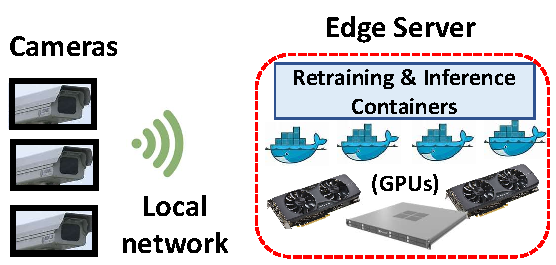
\includegraphics[width=0.6\columnwidth]{ekya/figures/xxx_cropped.pdf}
     \caption{Cameras connect to the edge server, with consumer-grade GPUs for DNN inference and retraining containers.%. We propose extending the workload to include continuous retraining of DNNs.
     }
     \label{fig:edge}
 \end{figure}

Thus, due to reasons of network cost and video privacy, it is preferred to run both inference and retraining on the edge compute device itself without relying on the cloud. In fact, with bandwidths typical in edge deployments, cloud-based solutions are slower and result in lower accuracies (\S\ref{subsec:eval-alternate}).

\subsection{Compressed DNN models and data drift}
\label{subsec:continuous}

Advances in computer vision research have led to high-accuracy DNN models that %surpass human-level accuracy on general images and videos. These DNN models 
achieve high accuracy with a large number of weights, deep architectures, and copious training data. While highly accurate, using these heavy and general DNNs for video analytics is both expensive and slow \cite{noscope, DBLP:conf/osdi/HsiehABVBPGM18}, which make them unfit for resource-constrained edge computing. The most common approach to addressing the resource constraints on the edge is to train and deploy \emph{specialized and compressed} DNNs \cite{compression-4, compression-5, compression-6, compression-17, compression-18, compression-19}, which consist of far fewer weights and shallower architectures. \revtext{For instance, Microsoft's edge video analytics platform ~\cite{rocket-blog} uses a compressed DNN (TinyYOLO~\cite{redmon2018yolov3}) for efficiency. Similarly, Google released Learn2Compress\cite{learn2compress} for edge devices to automate the generation of compressed models from proprietary models.} These compressed DNNs are trained to only recognize the limited objects and scenes specific to each video stream. In other words, to maintain high accuracy, they forego generality for improved compute efficiency \cite{noscope, DBLP:conf/osdi/HsiehABVBPGM18, mullapudi2019}. 

% use cases - connected smart cars, indexing on iphone, even stationary traffic cameras
%Advances in DNN efficiency, e.g., using model compression \cite{compression-4, compression-5, compression-6, compression-17, compression-18, compression-19}, have enabled the deployment of DNN models on resource-constrained edge servers. Efficient edge models drive video analytics applications in modern cars, urban mobility traffic control, and enterprise campuses \cite{bellevue-report}. %Video analytics in smart cars already provide safety assist features (e.g., lane drift alerts) and many more such features are expected in the near future \cite{smart-cars}. Camera streams in enterprise buildings are analyzed for security applications as well as for ubiquitous sensing applications, e.g., face recognition to authenticate building access \cite{smart-buildings}. %Mobile devices use DNN object classifiers to generate ``tags'' for the pictures and videos clicked by users, thus enabling search by keywords (e.g., find pictures with a party hat) \cite{iphone-indexing}. 
%\junchen{this para could be a good fit to a new subsection of ``DNN deployed at the edge''?}
%\junchen{i like the idea of starting with data drift, though maybe we should motivate why data drift is so damaging in the first place? }

%\begin{figure}[t!]
%  \centering
%  \begin{subfigure}[t]{0.5\linewidth}
%    \centering
%    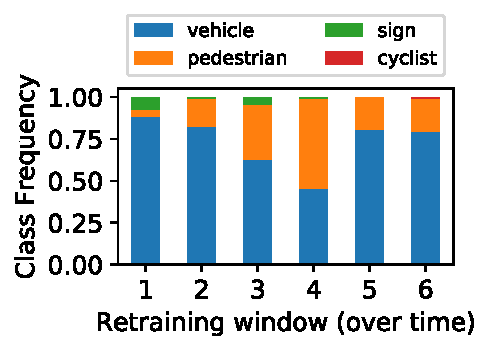
\includegraphics[width=\linewidth]{ekya/ekya/figures/motivation/incr_learn_motivation/motivation_waymo_distchange_classdist.pdf} 
%    \caption{Class distribution}
%    \label{fig:class-distrib-motivation}
%  \end{subfigure}
%  ~~~
%  \begin{subfigure}[t]{0.5\linewidth}
%    \centering
%    % 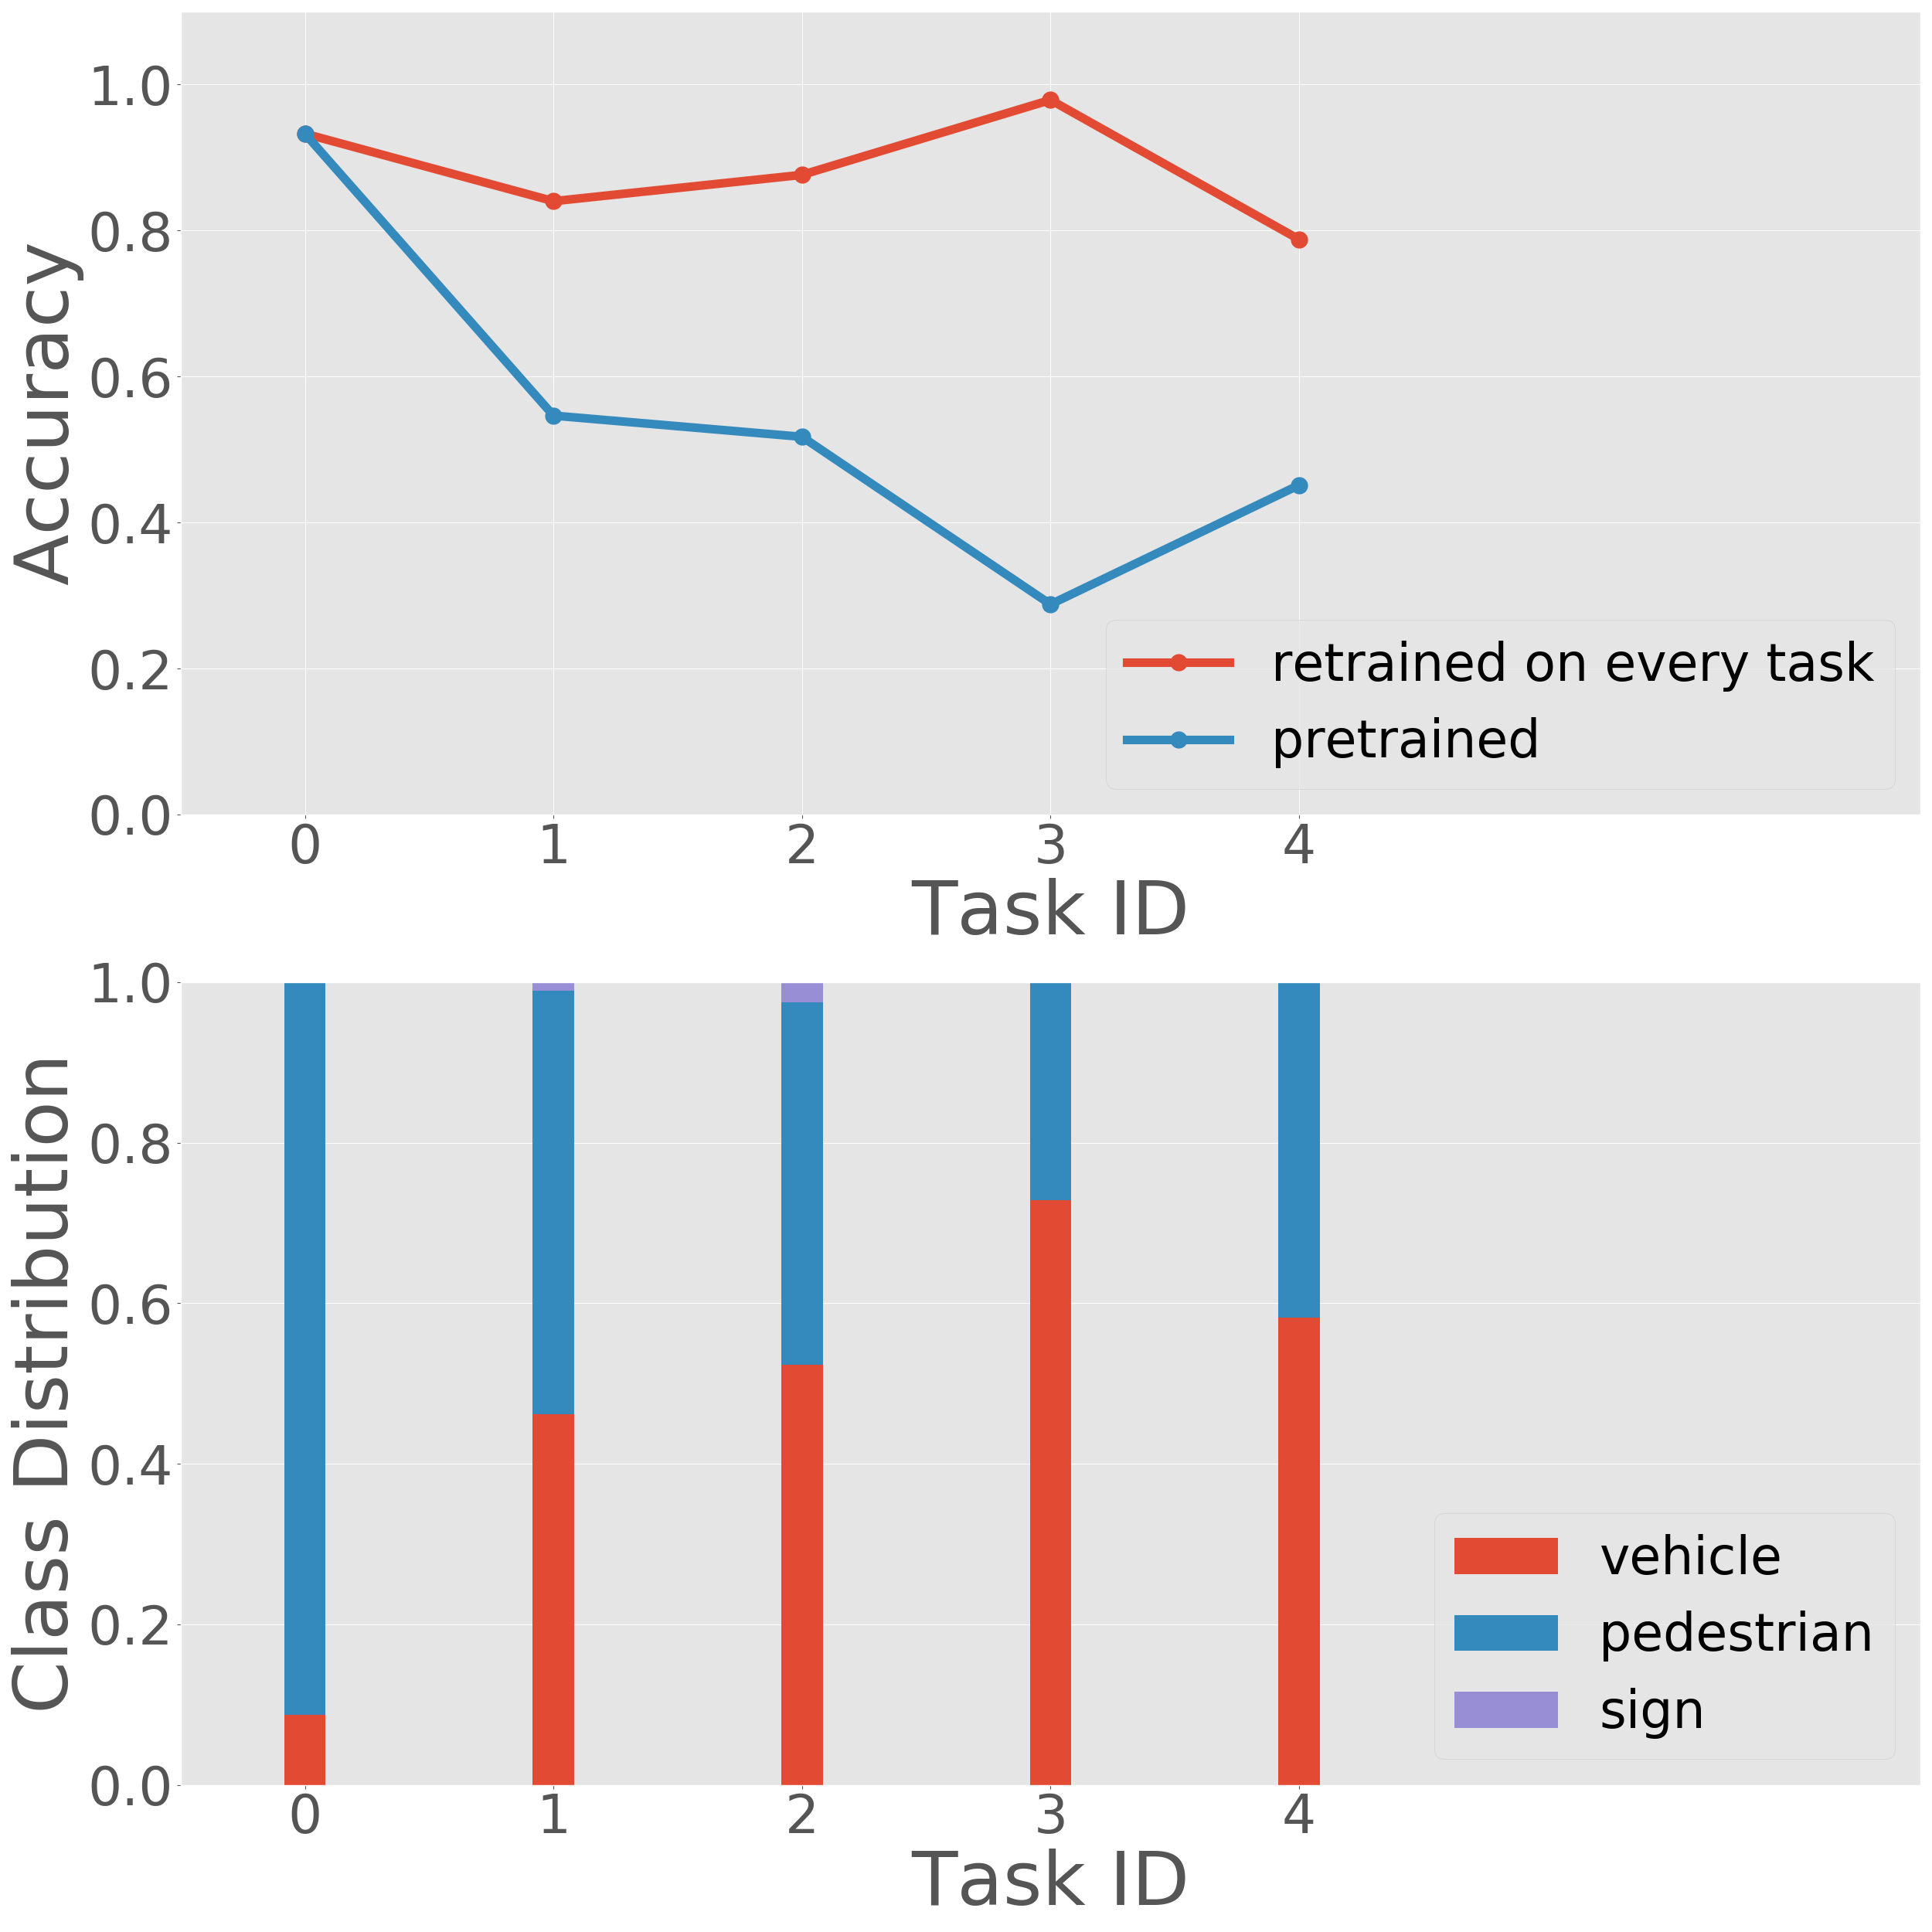
\includegraphics[width=\linewidth]{ekya/figures/motivation/Class_Incrementality/class_distribution_change_sf_27.png}
%    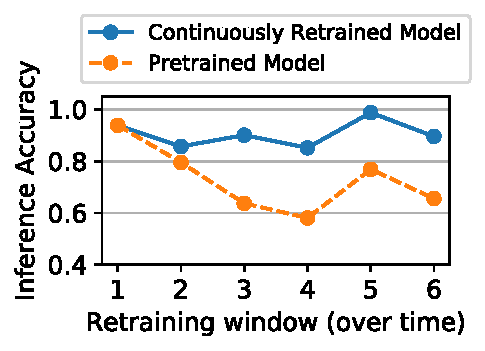
\includegraphics[width=\linewidth]{ekya/figures/motivation/incr_learn_motivation/motivation_waymo_distchange_acc.pdf}
%     \caption{Accuracy}
%    \label{fig:class-distrib-motivation-acc}
%  \end{subfigure}
%  \caption{Impact of changing class distribution (left) on model accuracy in the Waymo data. Continuous learning results in higher and steady accuracy over time (right). \kh{Update the figures to include the one trained with first half of the tasks}}
%  \label{fig:waymo-motivation-distrib}
%\end{figure}


\noindent{\bf Data drift.} As specialized edge DNNs have shallower architectures than general DNNs, they can only memorize limited amount of object appearances, object classes, and scenes. As a result, specialized edge DNNs are particularly vulnerable to {\em data drift} \cite{datadrift-7, datadrift-8, datadrift-a, datadrift-b}, where live video data diverges significantly from the initial training data. For example, variations in the object pose, scene density (e.g. rush hours), and lighting (e.g., sunny vs. rainy days) over time make it difficult for traffic cameras to accurately identify the objects of interest (cars, bicycles, road signs). Cameras in modern cars observe vastly varying scenes (e.g., building types, crowd sizes) as they move through different neighborhoods and cities. Further, the {\em distribution} of the objects change over time, which reduces the edge model's accuracy \cite{distribution-20, distribution-21}. Due to their ability to memorize limited amount of object variations, edge DNNs have to be continuously updated with recent data and changing object distributions to maintain a high accuracy.  %Finally, newer object classes may appear (e.g., segway scooters) which may not have been available in the initial training data \cite{incremental-24, icarl-14}.  

%\vspace{-.05in}\subsubsection{\bf Data drift.} %While model compression has considerably increased the inference efficiency of DNN models, it also results in their having lower ``capacity'' to learn from their training data. 
%While compressed models are initially trained on representative data, when they are out in the field, they suffer from {\em data drift} \cite{datadrift-7, datadrift-8, datadrift-a, datadrift-b}. Data drift refers to the live video data diverging significantly from the initial training data. For example, traffic cameras encounter many variations in the angles of objects, scene density, and lighting over time, thus making it difficult to accurately identify the objects of interest (cars, bicycles, road signs).  
%Cameras in modern cars observe vastly varying scenes (e.g., building colors, crowd sizes) as they move through different neighborhoods and cities. %\ion{Are we considering cameras in slefdriving cars? If yes, I'm not sure about it. First, cars can have very powerful processors. Second, I don't think that we can easily sell the point about degrading inference to do the training in such a mission critical app (just add a second processor for inference). Third, not sure we want to deploy a model in a self-driving car without careful validation.} 


%The problem of data drift is exacerbated in compressed models. Compression of DNNs makes them efficient in their compute and memory demands, and facilitates their deployment on resource-constrained edge servers. However, smaller DNNs can memorize less due to their relatively limited capacity. In other words, their efficiency comes at the expense of generalizability to the data distributions of live inference videos that are different than their training data \cite{compressiondrift-22, compressiondrift-23, efficientnet-3}. %It is generally difficult to provide an exhaustive training dataset with enough samples to cover all possible variations.
%It is difficult and often intractable to provide an exhaustive training dataset with enough samples to cover all possible variations, especially in open real-world deployments. 

%\ga{Model capacity drops due to compression?} \junchen{to Ganesh's comment on compression vs. capacity: totally agree this is what any (knowledgeable) reviewer may wonder as well. i believe there {\em is} a fundamental tradeoff between capacity (how much to compress) and generalizability (robustness to data drift).maybe just cite the ECCV paper Romil found and ask Nikolas for more.} \ys{+1 on this point. The large the model is, the higher capacity it has. However, a large model not only requires a huge amount of data and time for training, but also leads to a higher runtime cost (memory, latency etc.) during inference. Hence, an alternative of having a large well-trained model is to maintain a localized cheaper model, and retrain it on demand. }

\noindent{\bf Continuous training.} The preferred approach, that has gained significant attention, is for edge DNNs to {\em continuously learn} as they incrementally observe new samples over time \cite{incremental-13, icarl-14, incremental-15}. %while not fully forgetting the learnings from old samples. 
The high temporal locality of videos allows the edge DNNs to focus their learning on the most recent object appearances and object classes \cite{DBLP:conf/cvpr/ShenHPK17, mullapudi2019}.  
%Incremental learning techniques %retain snapshots of history for the retraining (not the entire historical dataset) and  avoid {\em catastrophic forgetting} of the learnings on historical data \cite{datadrift-8} even as they learn from new data. 
%In \name, we use a modified version of iCaRL \cite{icarl-14} though our techniques are generally applicable.
In \name, we use a modified version of iCaRL\cite{icarl-14} learning algorithm to on-board new classes, as well as adapt to the changing characteristics of the existing classes. %We also tune the balance distillation and cross-entropy losses. 
%We use the iCaRL \cite{icarl-14} incremental learning algorithm for our experiments though the techniques in our work are generally applicable.
%In our solution, 
Since manual labeling is not feasible for continuous training systems on the edge, \revtext{the labels for the retraining are obtained from a ``golden model'' - a highly accurate (87\% and 84\% accuracy on Cityscapes and Waymo datasets, respectively) but expensive model (deeper architecture with large number of weights)}. The golden model cannot keep up with inference on the live videos and we use it to label only a small fraction of the videos in the retraining window. %\revtext{We then use these labels from the golden model to train compressed models.} 
Our approach is essentially that of supervising a low-cost ``student'' model with a high-cost ``teacher'' model (or knowledge distillation \cite{44873}), and this has been broadly applied in computer vision literature \cite{incremental-13, mullapudi2019, incremental-15, distribution-20}. %The use of a golden model for labeling is consistent with prior work in computer vision literature \cite{incremental-13, mullapudi2019, incremental-15, distribution-20}. 


% data drift; class incremental; waymo graphs; app-level impact
\subsection{Accuracy benefits of continuous learning}
\label{subsec:continuous-measurement}

\begin{figure}[t!]
  \centering
  % Accuracy figure
  % Class distribution figure
  \begin{subfigure}[t]{0.42\linewidth}
    \centering
    % 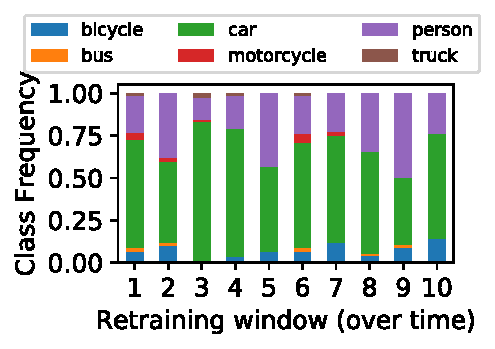
\includegraphics[width=\linewidth]{ekya/figures/motivation/incr_learn_motivation/motivation_jena_classdist.pdf}
    % 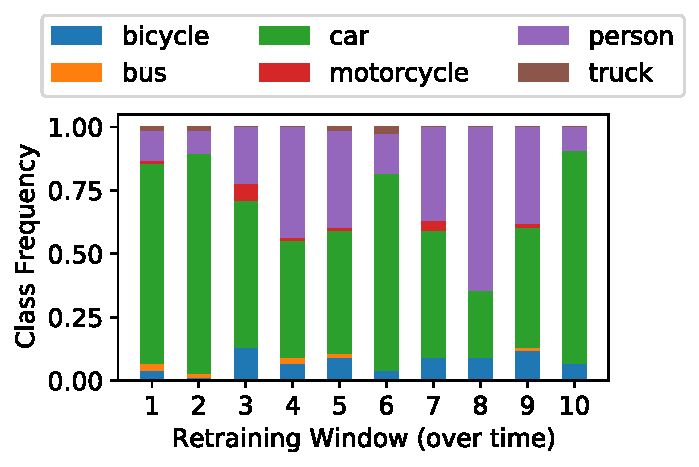
\includegraphics[width=\linewidth]{ekya/figures/motivation/incr_learn_motivation/motivation_cityscapes_jena_classdist.pdf}
    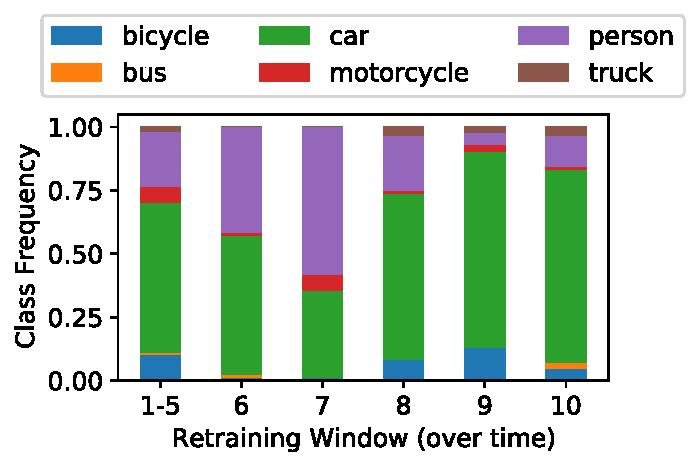
\includegraphics[width=\linewidth]{ekya/figures/motivation/incr_learn_motivation/motivation_cityscapes_zurich_classdist.pdf}
    \caption{Class Distribution}
    \label{fig:jena-classdist}
  \end{subfigure}
    ~~
  \begin{subfigure}[t]{0.42\linewidth}
    \centering
    % 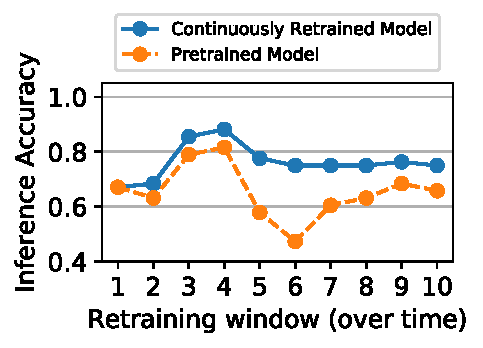
\includegraphics[width=\linewidth]{ekya/figures/motivation/incr_learn_motivation/motivation_jena_acc.pdf}
    % 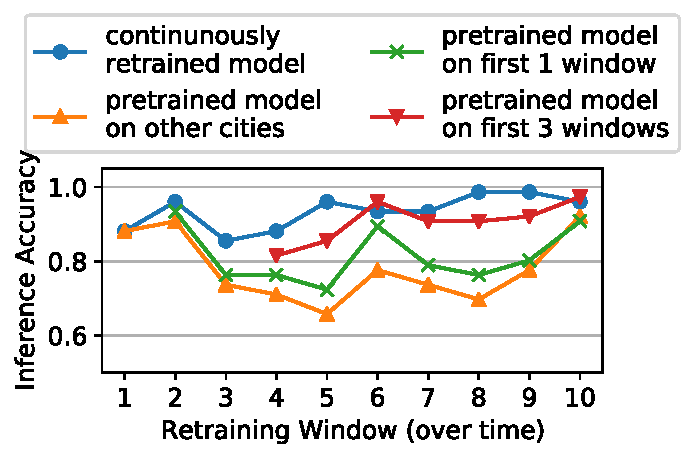
\includegraphics[width=\linewidth]{ekya/figures/motivation/incr_learn_motivation/motivation_cityscapes_jena_accuracy.pdf}
    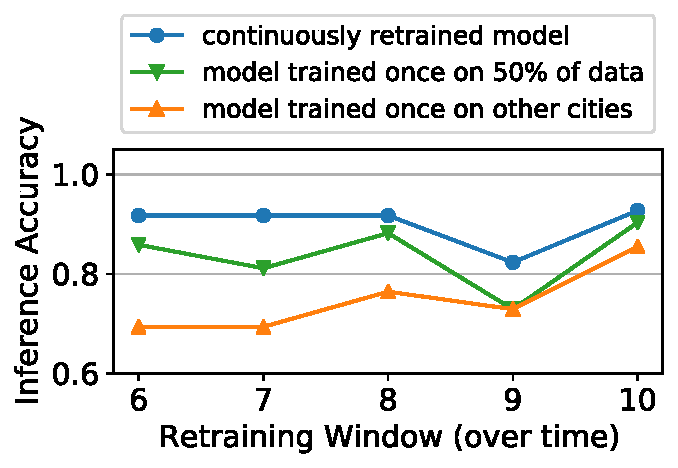
\includegraphics[width=\linewidth]{ekya/figures/motivation/incr_learn_motivation/new_motivation_cityscapes_zurich_accuracy.pdf}
    
    
    \caption{Accuracy}
    \label{fig:jena-motivation}
  \end{subfigure}
    \hspace*{\fill}
  ~~
  % Sample Image Task 1
  \begin{subfigure}[t]{0.41\linewidth}
    \centering
    % 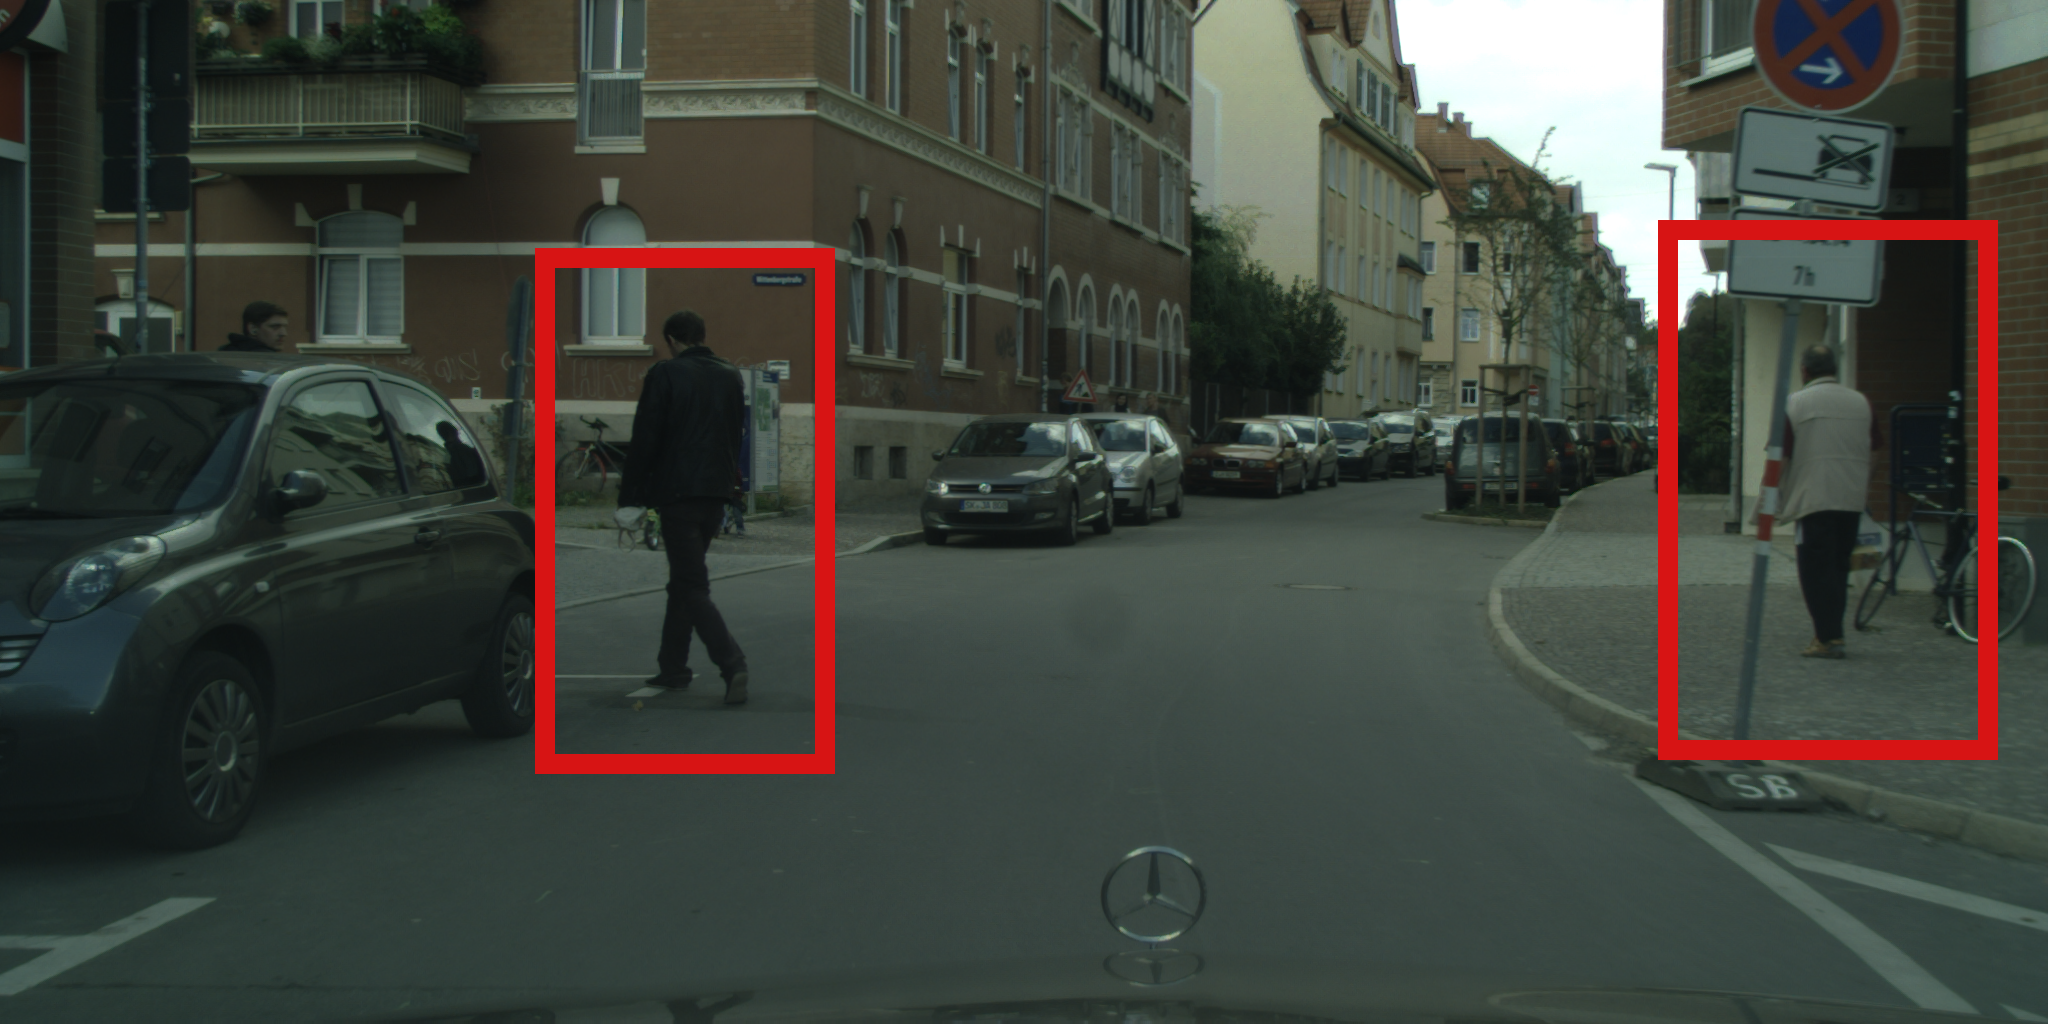
\includegraphics[width=\linewidth]{ekya/figures/motivation/incr_learn_motivation/t1_marked.png}
    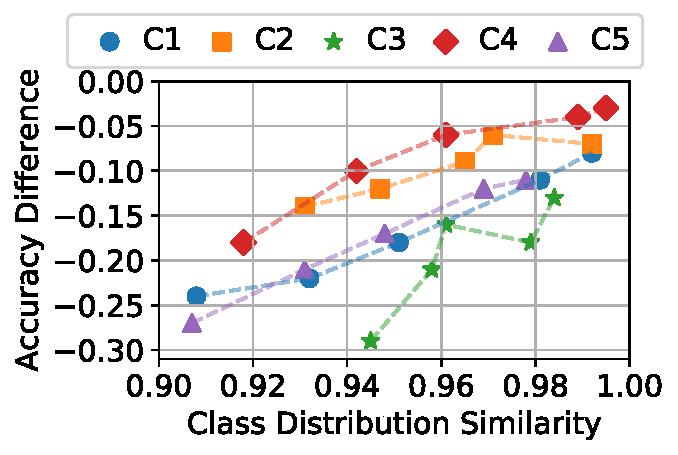
\includegraphics[width=\linewidth]{ekya/figures/motivation/incr_learn_motivation/motivation_datadrift_vs_acc.pdf}
     \caption{Accuracy vs data drift}
    \label{fig:acc-datadrift}
  \end{subfigure}
  ~~
  % Sample Image Task 6
  \begin{subfigure}[t]{0.41\linewidth}
    \centering
    % 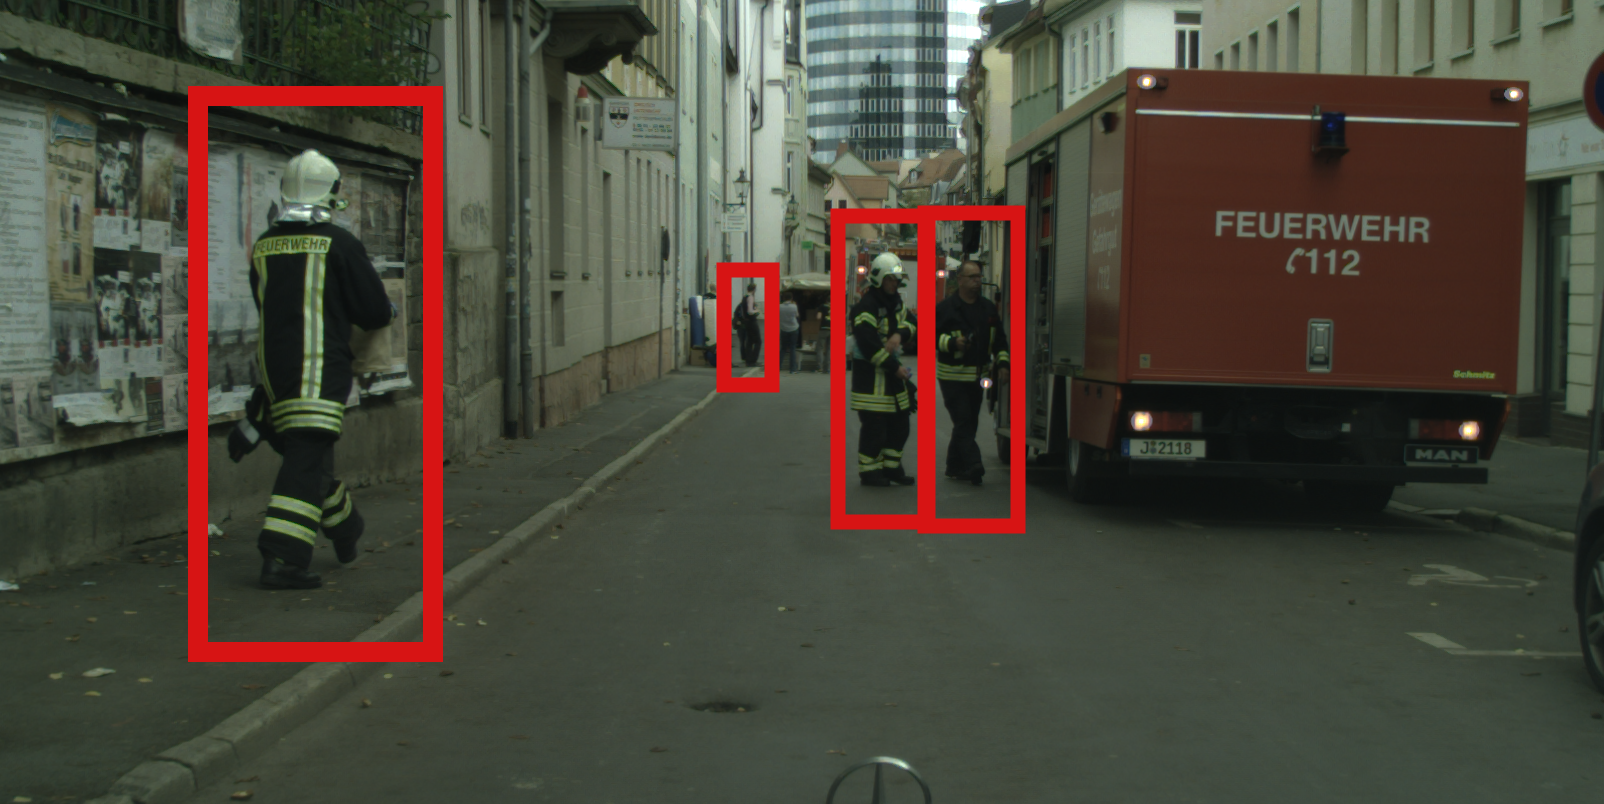
\includegraphics[width=\linewidth]{ekya/figures/motivation/incr_learn_motivation/t6_marked.png}
    % 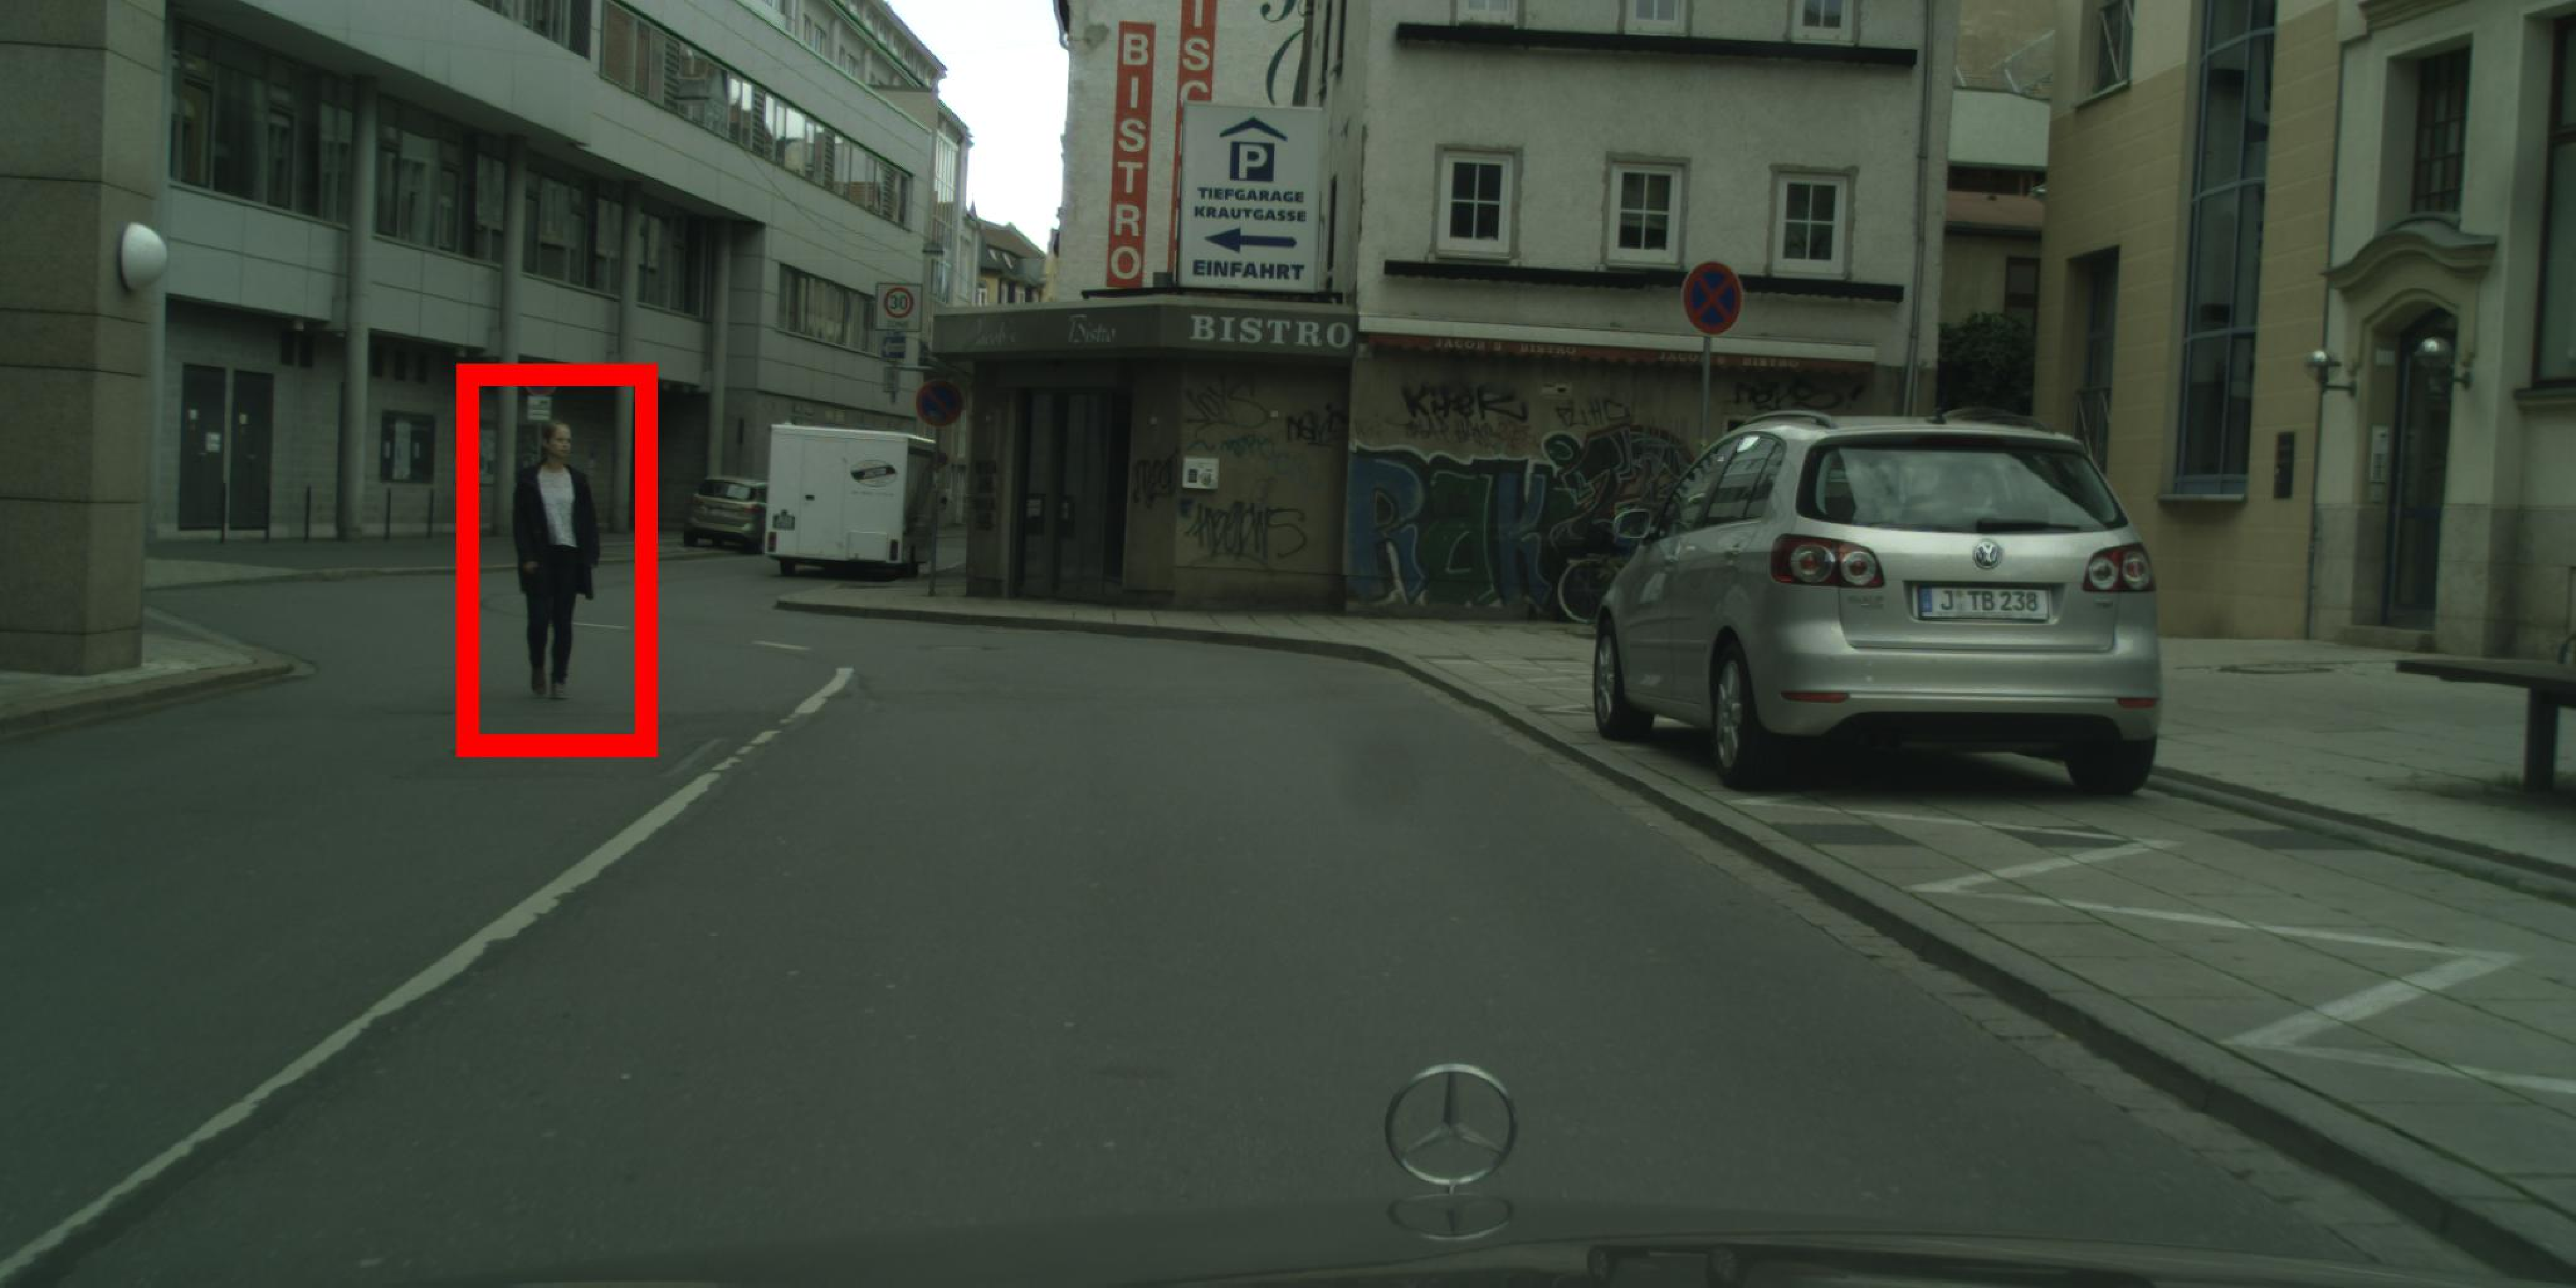
\includegraphics[width=\linewidth]{ekya/figures/motivation/incr_learn_motivation/motivation_cityscapes_jena_win5.pdf}
    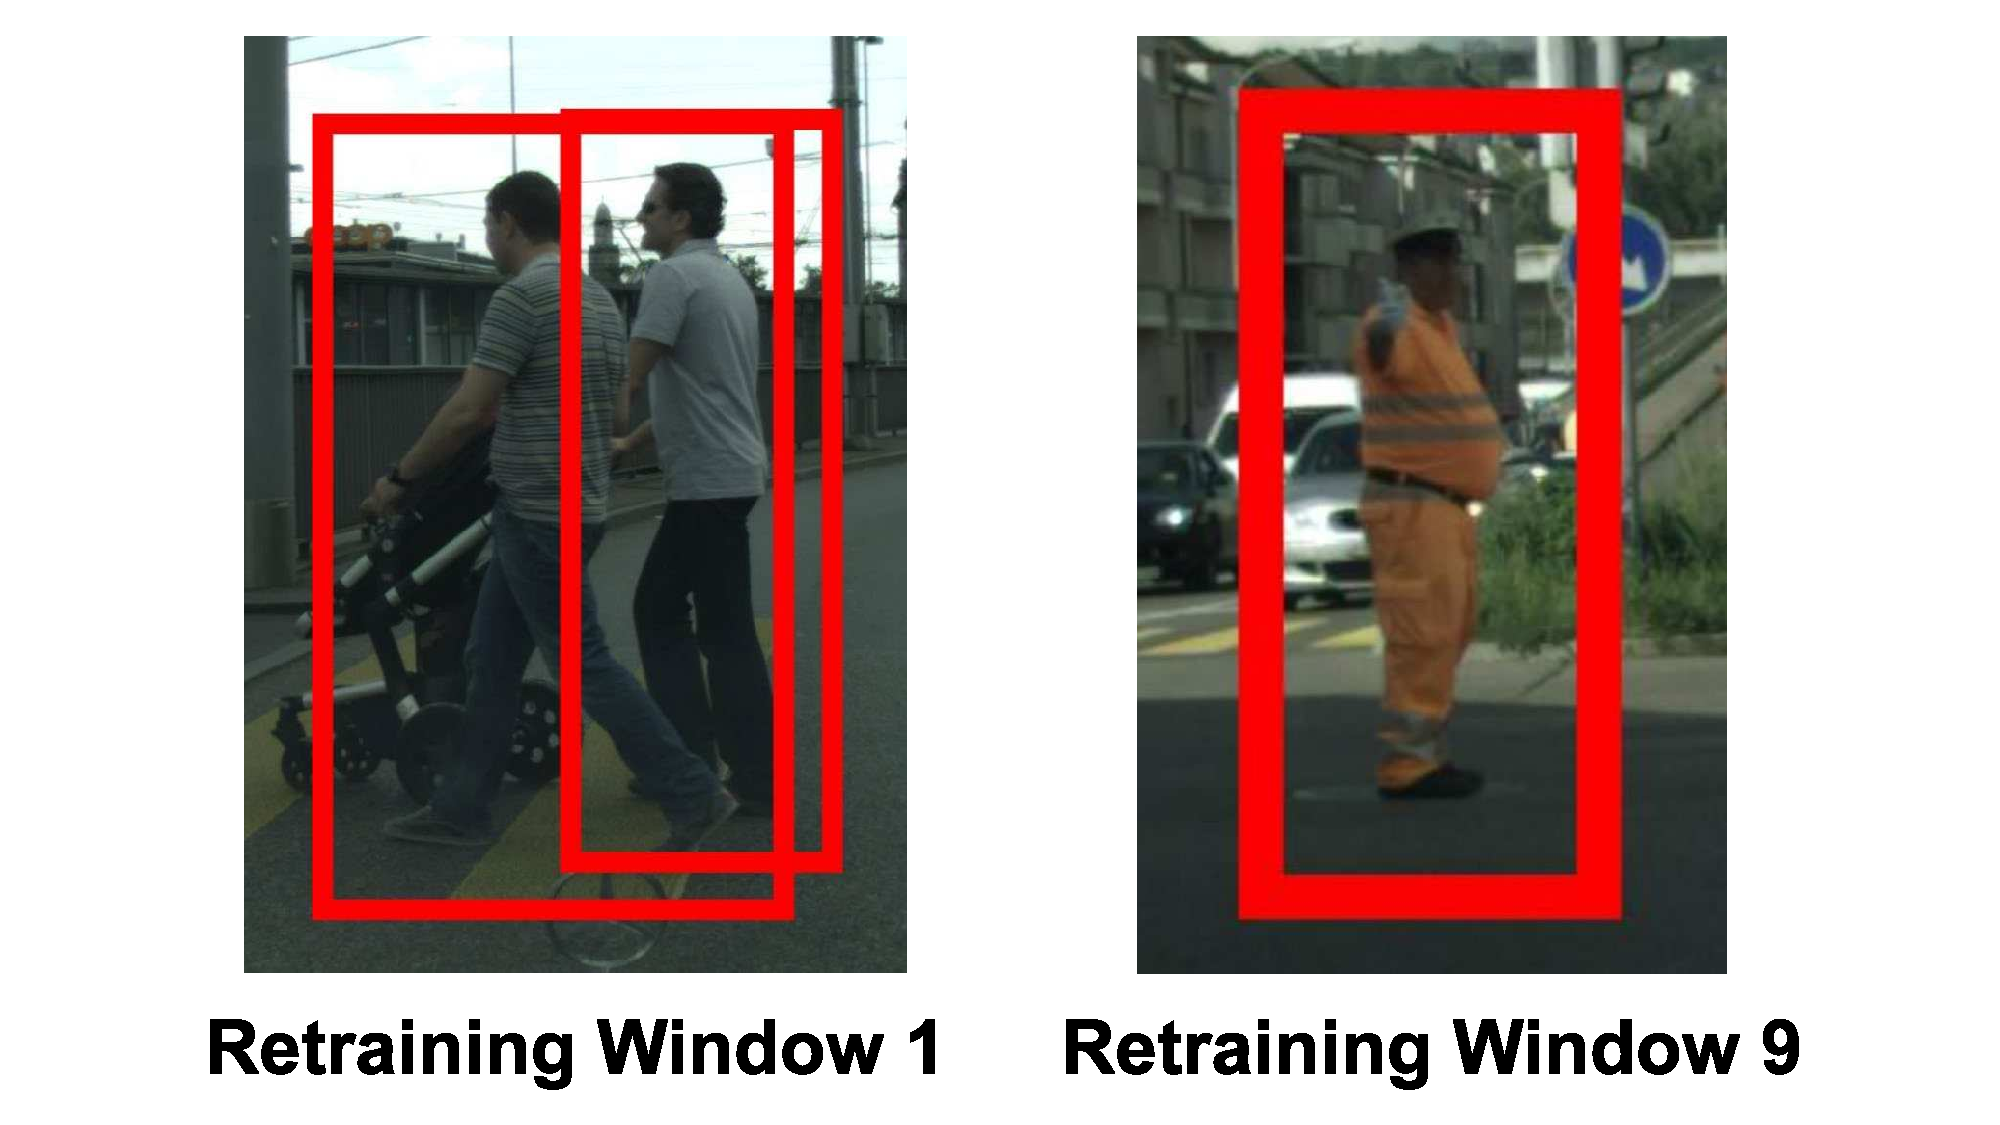
\includegraphics[width=\linewidth]{ekya/figures/motivation/incr_learn_motivation/person_classshift.pdf}
    \caption{Person class variations}
    \label{fig:personclass}
  \end{subfigure}
  
   \caption{\cameratext{Continuous learning in the Cityscapes dataset. Shift in class distributions (a) across windows necessitates continuous learning (b). Model accuracy is not only affected by class distribution shifts (c), but also by changes in object appearances (d).}}% As more data samples are made available to model for retraining, it achieves a higher accuracy compared to a pre-trained model which does not adapt to the new data samples. We evaluate the accuracy of the following classes -- 'person', 'car, 'truck', 'bus', 'bicycle', 'motorcycle'.}
  \label{fig:cityscapes-motivation}
\end{figure}



%To show the benefits of continuous learning, we use two video datasets that were collected from dashboard cameras in cars: Cityscapes \cite{cityscapes} in Europe and Waymo \cite{waymo} in the USA. These cameras collect data samples over time and at different locations. (Details of the datasets in \S\ref{subsec:eval-setup}). 

To show the benefits of continuous learning, we use the video stream from one example city in the Cityscapes dataset \cite{cityscapes} that consists of videos from dashboard cameras in many cities. %over time and at different locations. 
In our evaluation in \S\ref{sec:evaluation}, we use both moving dashboard cameras as well as static cameras over long time periods. 
We divide the video data in our example city into ten fixed \emph{retraining windows} (200s in this example). 


\noindent\cameratext{\textbf{Understanding sources of data drift.} Figure \ref{fig:jena-classdist} shows the change of object class distributions across windows. The initial five windows see a fair amount of persons and bicycles, but bicycles rarely show up in windows 6 and 7, while the share of persons varies considerably across windows $6-10$. Figure~\ref{fig:acc-datadrift} summarizes the effect of this data drift on model accuracy in five independent video streams, C1-C5. For each stream, we train a baseline model on the first five windows, and test it against five windows in the future and use cosine similarity to measure the class distribution shift for each window. Though accuracy generally improves when the model is used on windows with similar class distributions (high cosine similarity), the relationship is not guaranteed (C2, C3). This is because class distribution shift is not the only form of data drift. Illumination, pose and appearance differences also affect model performance (e.g. clothing and angles for objects in the person class vary significantly; Figure \ref{fig:personclass}).}

\noindent\cameratext{\textbf{Improving accuracy with continuous learning.}} Figure \ref{fig:jena-motivation} plots inference accuracy of an edge DNN (a compressed ResNet18 classifier) in the last five windows using different training options. 
%: (1) pretrain the model with representative data from \kh{10} other cities in the same dataset; (2) pretrain the model with recent history (the first five windows) in the same video; and (3) continuously retrain the model in every window. 
%$(1)$ Starting with an off-the-shelf ResNet18 model that was trained on the ImageNet dataset \cite{DBLP:journals/ijcv/RussakovskyDSKS15} and further tuned 
$(1)$ Training a compressed ResNet18 with video data on all other cities of the Cityscapes dataset does not result in good performance.
%Note that tuning off-the-shelf models using related datasets is common in deployments. 
$(2)$ Unsurprisingly, we observe that training the edge DNN once using data from the first five windows {\em of this example city} improves the accuracy. %by $9\%$ on average. 
$(3)$ %However,  
%We observe that the pretrained model using all data from \kh{4} other cities performs poorly. Similarly, using data from the first five windows to pretrain the edge DNN also suffers from accuracy drops in the next five windows. Both results show the limitation of pretraining edge DNNs with large and representative data.  
%In contrast, 
{\em Continuous retraining} using the most recent data for training achieves the highest accuracy consistently. Its accuracy is higher than the other options %first two offline training options 
by up to $22\%$.%$ $15\%$ and $6\%$, respectively.  %and its accuracy is much higher and more consistent. 
%Its accuracy is up to \kh{$25\%$} higher than the pretrained DNNs in one window. On average across all windows, continuous retraining leads to \kh{$10\%$ to $20\%$} higher accuracy over the pretrained DNNs. 

\revtext{Interestingly, using the data from the first five windows to train the larger ResNet101 DNN (not graphed) achieves better accuracy than the continuously retrained ResNet18.}  %While this gap indicates the %presence of data drift and the 
%benefit of using the most recent data for training, 
The substantially better accuracy of ResNet101 compared to ResNet18 when trained {\em on the same data} of the first five windows also shows that this training data was indeed fairly representative. But the lightweight ResNet18's weights and architecture limits its ability to learn and is a key contributor to its lower accuracy.
%This shows that the data in the first five windows is in fact fairly representative, but the ResNet18 model's cheaper weights and architecture is a key factor contributing to its lower accuracy. 
Nonetheless, ResNet101 %is unsuited for live video inference as it takes $50-260$ms per inference on edge class GPUs \cite{cnn-perf}, which 
is $13\times$ slower than the compressed ResNet18 \cite{cnn-perf}. % which makes the latter more suited for edge deployments.
%cost of $50-260$ms per inference on edge class GPUs 
%. 
This makes the efficient ResNet18 more suited for edge deployments and continuous learning enables it to maintain high accuracy even with data drift. Therefore, the need for continuous training of edge DNNs is ongoing and not just during a ``ramp-up'' phase. %We use the even more expensive \gaa{ResNext101} as our golden model for labeling, and we have verified that its results almost match manual labeling.
% Efficiency between ResNet101 and ResNet18 Ref: https://github.com/jcjohnson/cnn-benchmarks
% Our measured 
% is unable to memorize all the data.



%even though the edge DNN is pretrained with \kh{10$\times$} of data samples from the same dataset.  
%As Figure \ref{fig:jena-classdist} shows, class distribution changes quickly over time. The initial training samples are dominated by vehicles, but a lot more pedestrians and motorcycles show up at later time. 
%The appearance of objects also changes significantly, such as pedestrians show up in different clothing and angles at different time (Figure \ref{fig:jena-image-1} and \ref{fig:jena-image-6}).
%Figure \ref{fig:jena-motivation} shows that such data shift causes major accuracy drop for edge DNNs (ResNet18 in this example) that are pretrained with data from other cities. 
%We also see considerable accuracy drop even when the edge DNN is retrained with the same video in the first one and first three windows.


%Retraining window $6$ in Figure \ref{fig:cityscapes-motivation} highlights an interesting aspect. The distributions of classes in window \kh{$6$} and window \kh{$1$} are similar (Figure \ref{fig:jena-classdist}), yet the continuously retrained model achieves much higher accuracy than the model that is pretrained with data in window \kh{$1$} (Figure \ref{fig:jena-motivation}). Visual inspection suggests that this difference is likely due to the varying appearance and angles of objects (e.g., people with different clothing) between the two windows; see Figures \ref{fig:jena-image-1} and \ref{fig:jena-image-6}.% Thus, continuous learning is valuable even when the class

%Figure \ref{fig:waymo-motivation-distrib} illustrates how class distribution and DNN inference accuracy change over time in one city in the Waymo dataset, and the results are shown in fixed \emph{retraining windows} (\kh{xx} seconds in this example). 
%As Figure \ref{fig:class-distrib-motivation} shows, class distribution changes significantly over time. The initial training samples are dominated by vehicles, but a lot more pedestrians and road signs show up at later time. 
%As Figure \ref{fig:class-distrib-motivation-acc} shows, this data shift causes major accuracy drop for edge DNNs (ResNet18 in this example) that are pretrained with offline data in the same dataset. 
%We also see considerable accuracy drop even when the edge DNN is retrained with the \emph{first half} of the video in this camera.
%In contrast, the continuously retrained DNN keeps using recent data to cope with the changing distributions, and it achieves \kh{$xx\%$ and $yy\%$} higher accuracy over the DNNs that are pretrained with the offline and first half video data, respectively. We observe similar phenomenon in all other cities in the Waymo dataset, as continuously retrained edge DNNs achieve \kh{xx\%} higher accuracy over pretrained edge DNNs on average (up to \kh{yy\%}). \footnote{In Figures \ref{fig:waymo-motivation-distrib} and \ref{fig:cityscapes-motivation}, at each retraining window $i$ on the x-axis, the data from ($i-2, i-1$) is used for retraining the model, and the data from ($i-1, i$) is used for inference (testing), whose accuracy in turn is plotted on the y-axis.}

%Figure \ref{fig:class-distrib-motivation} demonstrates the impact of changes to the distribution of object classes in (a single city of the Waymo data) on the ResNet18 classifier. We compare the accuracies of a continuously updated ResNet18 classifier against the version of ResNet18 that was pre-trained only once initially (on a few samples from this video). 
%Further, continuous learning is also beneficial when the {\em distribution} of data samples of the object classes changes over time; Figure \ref{fig:class-distrib-motivation}. 
%While the initial training samples are dominated by vehicles, more examples of pedestrians  and road signs become available with time (Figure \ref{fig:class-distrib-motivation}). This is typical of video data in suburban cities where the pedestrian traffic is considerably lower than vehicular traffic. The changing distribution causes the once-trained ResNet18's accuracy to drop while the continuously trained model keeps retraining itself with the recent data, copes with the changing distributions, and achieves $28\%$ higher accuracy (Figure \ref{fig:class-distrib-motivation-acc}). \footnote{In Figures \ref{fig:waymo-motivation-distrib} and \ref{fig:cityscapes-motivation}, at each retraining window $i$ on the x-axis, the data from ($i-2, i-1$) is used for retraining the model, and the data from ($i-1, i$) is used for inference (testing), whose accuracy in turn is plotted on the y-axis.}




% sample incremental; jena and tubingen of cityscapes
%Figure \ref{fig:cityscapes-motivation} shows the benefits of {\em sample-incremental} training, i.e., improving the model with newer data samples over time. %We use two videos for this experiments from cars driving in two cities, Jena and Tubingen. 
%We compare the accuracies of the continuously updated ResNet18 convolutional classifier against the version of ResNet18 that was trained only once initially (on a few representative samples before the edge model was deployed). 

%Figure \ref{fig:cityscapes-motivation} shows the similar phenomenon of the impact of changing class distributions (Figure \ref{fig:jena-classdist}) with the Cityscapes data (again, a single city). 
%As Figure \ref{fig:jena-motivation} shows, continuously retrained DNN achieves much higher (by \kh{$zz\%$}) and more steady accuracy than the pretrained DNNs.
%Across all cities in the Cityscapes dataset, continuously retrained DNNs achieve \kh{xx\%} higher accuracy over pretrained edge DNNs on average (up to \kh{yy\%} higher).
%while the accuracies of the two models -- continuously-trained and once-trained -- are similar at the beginning, over time, continuous learning leads to the model's accuracy being higher (by $27\%$) and relatively steady. % they diverge over time to a difference of as much as $27\%$ in accuracy. Continuous learning results in relatively steady (and higher) accuracy over time. %We observe a similar trend in Figure \ref{fig:tubingen-motivation} where the divergence in accuracy due to not updating the model is observed immediately. (Note that in each of Figure \ref{fig:jena-motivation} and \ref{fig:tubingen-motivation} our experiments use new data samples over time obtained from a {\em single} city.)  
%Retraining window $6$ in Figure \ref{fig:cityscapes-motivation} highlights an interesting aspect. The distributions of classes in window \kh{$6$} and window \kh{$1$} are similar (Figure \ref{fig:jena-classdist}), yet the continuously retrained model achieves much higher accuracy than the model that is pretrained with data in window \kh{$1$} (Figure \ref{fig:jena-motivation}). Visual inspection suggests that this difference is likely due to the varying appearance and angles of objects (e.g., people with different clothing) between the two windows; see Figures \ref{fig:jena-image-1} and \ref{fig:jena-image-6}.% Thus, continuous learning is valuable even when the class distributions are similar.

%%Comparing against a version of the model that is trained on representative data initially is conservative because typical deployments use off-the-shelf models that are pre-trained on standard datasets (e.g., ImageNet \cite{imagenet} or MS-COCO \cite{coco}). 
%%%%%Our experiments, overall, demonstrate the value of improving the models with new data samples to cope with changing data distributions as well as changing conditions and appearances of the objects. 
%\junchen{hmm.. i do see the point that having more samples helps, but in any event, people will use a model (even a cheap one) trained offline with some {\em large} standard dataset (imagenet, coco, etc). i tend to believe the gain is due to fine-tuning the ResNet model to in-situ data from the Cityscape ``scene'' and more such data the better?}
%%Continuous learning also helps to learn altogether new object classes, whose examples may not have been included in the training data \cite{incremental-24, icarl-14}.
%\noindent{\bf Rate of change.} Finally, different videos change at different rates. Urban settings typically observe higher change in their data distributions and will benefit from more frequent retraining, while suburban settings will do with a relatively lower retraining frequency. Likewise, times of busy traffic see a faster change in their data distributions compared to off-peak periods. In addition, the data distributions are also significantly different {\em across cities} (even if they are neighboring) in both the Waymo and Cityscapes datasets. Models that are deployed in vehicles moving across neighboring cities at different times will benefit from learning on new data. 

%We observe similar phenomenon across a diverse set of videos (see \S\ref{sec:evaluation}). Edge DNNs that are pretrained only once experience significant accuracy drop over time, even if their training data is from the same video in the recent history. These sharp accuracy drops make the inference results inconsistent and unreliable.  In contrast, continuous training enables edge DNNs to adapt with the most recent and relevant data, and it leads to much higher and more steady accuracy. 



%\begin{figure}[t!]
%  \centering
%  \begin{subfigure}[t]{0.5\linewidth}
%    \centering
%    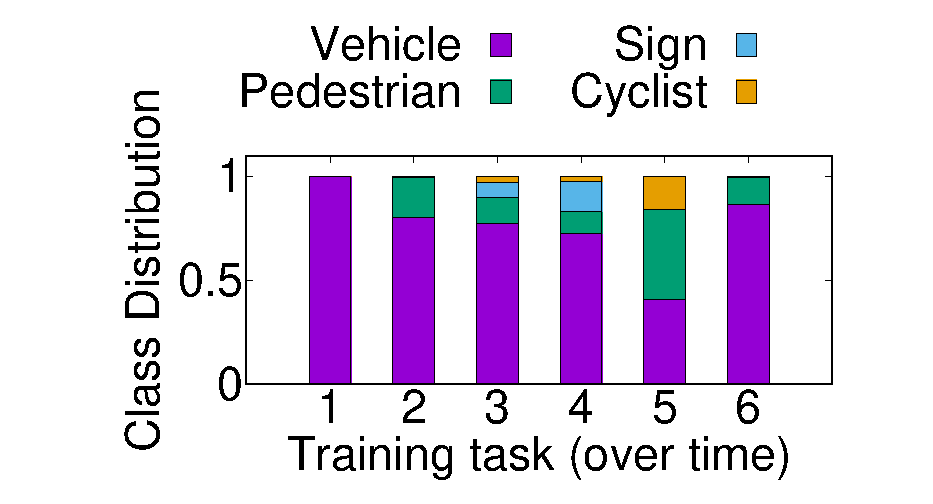
\includegraphics[width=\linewidth]{ekya/figures/motivation/Class_Incrementality/new_class.eps}
%    \caption{New classes over time}
%        \label{fig:class-inc-motivation}
%  \end{subfigure}
%  ~~
%  \begin{subfigure}[t]{0.5\linewidth}
%    \centering
%    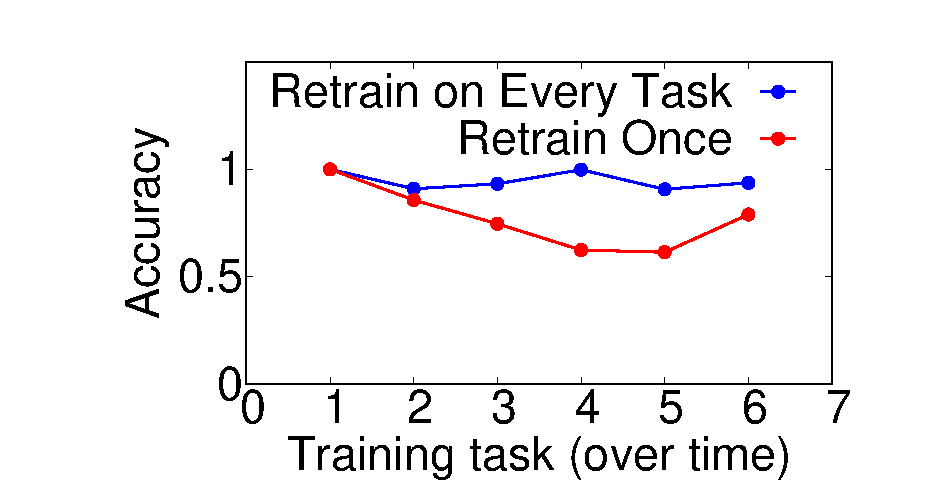
\includegraphics[width=\linewidth]{ekya/figures/motivation/Class_Incrementality/new_class_acc.eps}
%    \caption{Accuracy}
%        \label{fig:class-inc-motivation-acc}
%  \end{subfigure}
%   \hfill
%  ~~
%  \caption{Class incremental learning with Waymo.}
%  \label{fig:waymo-motivation}
%\end{figure}

%{\em Class-incremental} training refers to learning new object classes with time, thus expanding the model's classification targets. As shown in Figure \ref{fig:class-inc-motivation}, the initial training data only consists of samples of vehicles, but over time, pedestrians, road signs, and cyclists are added. Continuously updating the ResNet18 model to include these new classes results in consistently higher accuracy by as much as $37\%$ (Figure \ref{fig:class-inc-motivation-acc}). \ion{This example is a bit contrived. Why would you even consider deploying a model for video traffic that is trained only on cars in the first place?}


% impact of different retraining frequencies - show variation across two cities
%\ga{TODO paragraph.} \textbf{Retraining Frequency.} As a model specializes for a specific data distribution, its performance on general data decreases.  Moreover, frequent retraining requires more resources, which may not be available and thus the model may be trained only for a shorter duration \romil{The inference-resource-opportunity-cost argument can also be put here, but is not reflected in the plots}. Thus, a high retraining frequency can reduce the model accuracy.
%\junchen{Is retraining too frequently lowers the accuracy because of more frames being dropped or because of retraining ending prematurely for lack of resource? if so, please make it explicit. i was confused as reader..}
%This is observed in \cref{fig:cologne-motivation} and \cref{fig:erfurt-motivation}, where having just 2 tasks \romil{Explain what a task is} has a mean accuracy of 70.4\% over the entire dataset, but decreases to 69.8\% when retrained over 10 tasks. Similar behavior for Erfurt (82.9\% vs 82.2\%). 


% golden model; can retain more info but is expensive; edge model's capacity is less but is cheaper to execute
% show graph - golden, edge w/ retraining, edge w/o retraining (for one of the above cities); both sample and class incremental
% romilb: a third line in figure 1 - (showing continuously high accuracy?) 

%\noindent{\bf Golden model.}



% used for inference already; we propose running training too; storage isn't a concern but compute is limited; the network is also a worry, so we cannot access the infinite compute in the cloud
%\subsection{\bf Joint inference and retraining on edge servers.}
%Our proposal is to extend the edge servers, which already performs video DNN inferences, to {\em include continuous training of the edge DNN models}. Edge servers already have capacity to store the limited amount of recent video data that is required for continuous retraining. However, its compute capacity is a concern as the edge server's compute is already provisioned for the DNN inference on live video streams. Since retraining is periodic, i.e., its compute requirements are bursty in nature, provisioning compute resources for retraining will lead to wasted utilization and increased cost (by as much as \gaa{XXX} in our experiments). For the reasons explained in \S\ref{subsec:edge} regarding bandwidth constraints and privacy sensitivities, transmitting the videos to the cloud for retraining is not preferred. 
%As we describe next, we develop techniques to minimize disruption to the inference while smartly allocating resources for continuous retraining. %maximize the eventual inference accuracy. 


\section{Scheduling retraining and inference jointly}
\label{sec:ekya_motivation}
% This section motivates the scheduler

%Our goal is to utilize continuous learning (\S\ref{subsec:continuous}, \S\ref{subsec:continuous-measurement}) to maximize edge DNN accuracy in the face of data drift. 
%As continuous learning is a promising approach for data shift, we 
We propose \emph{joint retraining and inference} on edge servers.
The joint approach utilizes resources better than statically provisioning compute for retraining. Since retraining is periodic \cite{distribution-20, mullapudi2019} with far higher compute demands than inference, static provisioning causes idling.  
Compared to uploading videos to the cloud for retraining, our approach has advantages in privacy (\S\ref{subsec:edge}), and network costs and accuracy (\S\ref{subsec:eval-alternate}).
%Our approach also ensures everything is completed on the edge, which has clear advantages in network costs and privacy (\S\ref{subsec:edge}) over transmitting the videos to the cloud for retraining. 
%Our proposal is to extend the edge servers, which already performs video DNN inferences, to {\em include continuous training of the edge DNN models}. Edge servers have the capacity to store the limited amount of recent video data that is required for continuous retraining. However, the edge server's compute is already provisioned for the DNN inference on live video streams. %Since retraining is periodic, i.e., its compute requirements are bursty in nature, provisioning compute resources for retraining will lead to wasted utilization and increased cost (by as much as \gaa{XXX} in our experiments). 
%Statically provisioning additional resources for retraining is wasteful since retraining is periodic \cite{distribution-20, mullapudi2019} %\ion{Cite something to support the statement that retraining is periodic} 
%Uploading videos to the cloud for retraining 
%For the reasons explained in \S\ref{subsec:edge} -- bandwidth constraints and privacy sensitivities -- transmitting the videos to the cloud for retraining is not preferred. In fact, our analysis in \S\ref{subsec:eval-alternate} shows that sending data to the cloud for retraining adds significant delays due to network overheads.

%We present the properties of the configurations for continuous training and inference on the DNNs (\S\ref{subsec:profiles}), and describe an example to motivate their joint scheduling (\S\ref{subsec:motivation-sched-example}).

%Joint retraining and inference involves complex trade-offs among retraining and inference jobs for many video streams. \S\ref{subsec:profiles} describes the tradeoffs in retraining and inference configurations, and \S\ref{subsec:motivation-sched-example} presents an example to illustrate the tradeoffs in configuration selection and resource allocation. %uses an example to illustrate the scheduling considerations in configuration selection and resource allocation. 

\begin{figure}[t]
  \centering
   \begin{subfigure}[t]{0.47\linewidth}
    \centering
    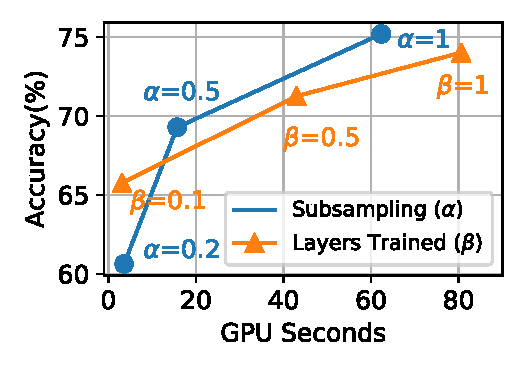
\includegraphics[width=\linewidth]{ekya/figures/motivation/AccuracyResourceProfile/jena_hypparams.pdf}
    \caption{Effect of Hyperparameters}
    \label{fig:hyparam-zoom}
  \end{subfigure}
  ~~~
  \begin{subfigure}[t]{0.48\linewidth}
    \centering
    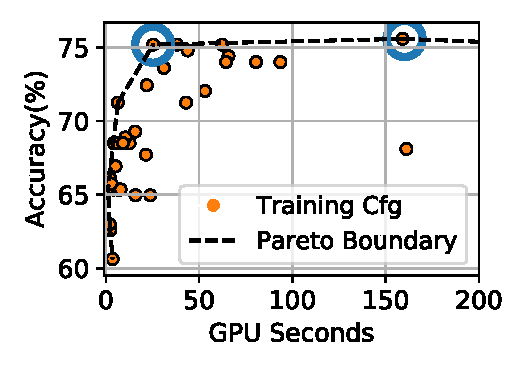
\includegraphics[width=\linewidth]{ekya/figures/motivation/AccuracyResourceProfile/jena.pdf}
    \caption{Resource-accuracy}
    \label{fig:darmstadt-profile}
  \end{subfigure}  
  \caption{Measuring retraining configurations. % with the Cityscapes dataset \cite{cityscapes}.
  GPU seconds refers to the duration taken for retraining with $100\%$ GPU allocation. (a) varies two example hyperparameters, keeping others constant. Note the Pareto boundary of configurations in (b); for every non-Pareto configuration, there is at least one Pareto configuration that is better than it in {\em both} accuracy and GPU cost. }
  \label{fig:resource-profiles}
\end{figure}


\subsection{Configuration diversity of retraining and inference}
\label{subsec:profiles}

%\ion{Actually, I think the last two subsections are part of the motivation, no?} 
\noindent{\bf Tradeoffs in retraining configurations.} The hyperparameters for retraining, or ``retraining configurations'', influence the resource demands and accuracy. %of the retrained model. 
Retraining fewer layers of the DNN (or, ``freezing'' more layers) consumes lesser GPU resources, as does training on fewer data samples, but they also produce a model with lower accuracy; Figure \ref{fig:hyparam-zoom}. %but yielding the maximum possible performance from the model may require training for a longer duration.

Figure \ref{fig:darmstadt-profile} illustrates the resource-accuracy trade-offs for an edge DNN (ResNet18) with various hyperparameters: number of training epochs, batch sizes, number of neurons in the last layer, number of frozen layers, and fraction of training data. We make two observations.
%We experiment with the following hyperparameters to retrain the ResNet18 classifier: number of epochs to train for, batch size, number of neurons in the last layer, number of layers to retrain, and the fraction of data between retraining windows to be used for retraining. We refer to every combination of these hyperparameter values as a {\em configuration}. Figure \ref{fig:resource-profiles} shows the spread among the hyperparameter configurations in their GPU resource usage and the accuracy of the retrained model.  
First, there is a wide spread in the resource usage (measured in GPU seconds), by upto a factor of $200\times$. 
%Some hyperparameter configurations lead to high accuracy but are expensive (top right of Figure \ref{fig:darmstadt-profile}), while some are cheap but lead to lower accuracy (bottom left of Figure \ref{fig:darmstadt-profile}). %Together, they form the Pareto boundary of configurations (\gaa{as marked}). 
Second, higher resource usage does not always yield higher accuracy. For the two configurations circled in Figure \ref{fig:darmstadt-profile}, their GPU demands vary by $6\times$ even though their accuracies are the same ($\sim 76\%$). Thus, careful selection of the configurations considerably impacts the resource efficiency.
% Connect this expt to 3b. Ideal - check if the pair of video-streams in 3b is similar/distinct.
\revtext{Moreover, the accuracy spread across configurations is dependent on the extent of data-drift. Retraining on visually similar data with little drift results in a narrower spread. % in accuracies.% across configurations.
}
%, To verify this, we retrained the same set of hyperparameters from Figure \ref{fig:darmstadt-profile} on a visually similar video segment as the test video segment (same time-of-day and city). Since the visual similarity results in a lower data-drift, the spread of accuracy values after retraining of the compressed models was much smaller - 6.2\%, compared to \fillme\% in Figure \ref{fig:darmstadt-profile}.}
With the changing characteristics of videos, it is challenging to efficiently obtain the resource-accuracy profiles for retraining.

% As the data drifts, if data is much more visually similar like the training configurations, the spread in accuracy is narrower for configurations


%{\em Changing profiles over time.} \romil{Talk about changing hyperparameter ordering.} \romil{Show that the profiles on the pareto boundary are predictable (or similar).}  % Changing profiles are fine as long as they are predictable.


\newcommand{\scell}[2][l]{%
  \begin{tabular}[#1]{@{}c@{}}#2\end{tabular}}
  
\begin{table}[t]
\centering
\addtolength{\tabcolsep}{-3pt}
\begin{tabular}{l cc cc}
\toprule
\multirow{2}{*}{\bf Configuration} & \multicolumn{2}{c}{\bf Retraining Window 1} & \multicolumn{2}{c}{\bf Retraining Window 2} \\
\cmidrule(lr){2-3} \cmidrule(lr){4-5}
& \scell{\bf End\\ \bf Accuracy} & \scell{\bf GPU\\ \bf seconds} & \scell{\bf End\\ \bf Accuracy} & \scell{\bf GPU\\\bf seconds} \\ \midrule
Video A Cfg1A       & 75    & 85    & 95    & 90      \\ \midrule
Video A Cfg2A (*)   & 70    & 65    & 90    & 40     \\ \midrule
Video B Cfg1B       & 90    & 80    & 98    & 80       \\ \midrule
Video B Cfg2B (*)   & 85    & 50    & 90    & 70\\ 
\bottomrule
\end{tabular}
\caption{\label{tab:schedmot-hypparams}Hyperparameter configurations for retraining jobs in Figure \ref{fig:schedmot}'s example. At the start of retraining window 1, camera A's inference model has an accuracy of 65\% and camera B's inference model has an accuracy of 50\%. Asterisk (*) denotes the configurations picked in Figures \ref{fig:schedmot-res-prioritization} and \ref{fig:schedmot-prioritization}.
%\romil{FIX: The GPU time cost between retraining windows cannot be different. The cost for the configs also be the same across videos. }
% \ion{Is 20\% a realistic accuracy? I mean at this accuracy the system is quite useless, no?}
}
\end{table}

% Scheduler motivation figure
\begin{figure}[t!]
  \centering
    \begin{subfigure}[t]{0.47\columnwidth}
    \centering
    %\hspace*{0.02in}
    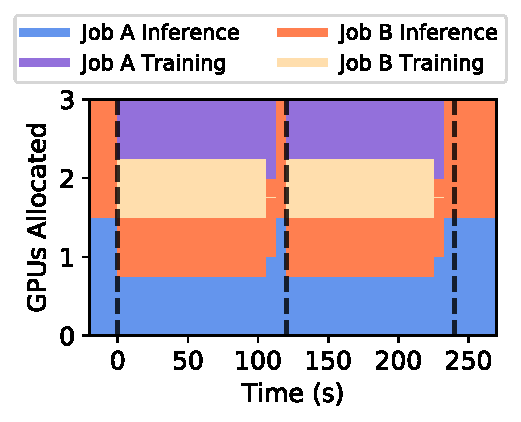
\includegraphics[width=\linewidth]{ekya/figures/motivation/Scheduler/schedmot_res_eventual_best_cfgs.pdf}
    \caption{Uniform scheduler}
    \label{fig:schedmot-res-naive}
  \end{subfigure}  
%  ~~
%  \begin{subfigure}[t]{0.3\linewidth}
%    \centering
%    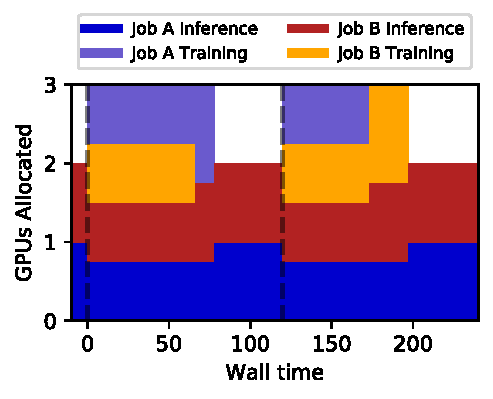
\includegraphics[width=\linewidth]{ekya/figures/motivation/Scheduler/schedmot_res_optimal_cfgs.pdf}
%    \caption{Optimal cfgs for retraining window}
%    \label{fig:schedmot-res-optimalcfg}
%  \end{subfigure}
  ~~
  \begin{subfigure}[t]{0.47\columnwidth}
    \centering
    %\hspace*{0.05in}
    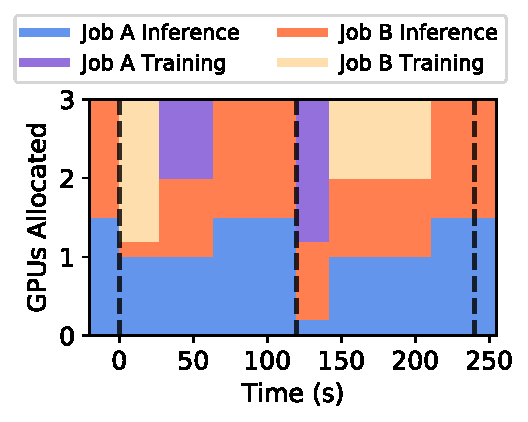
\includegraphics[width=\linewidth]{ekya/figures/motivation/Scheduler/schedmot_res_prioritization_and_optimal_cfgs.pdf}
    \caption{Accuracy-optimal scheduler}
    \label{fig:schedmot-res-prioritization}
  \end{subfigure}
      ~~\\
  \begin{subfigure}[t]{0.47\columnwidth}
    \centering
    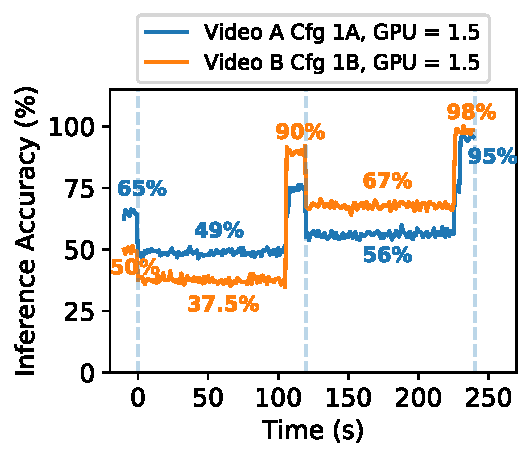
\includegraphics[width=\linewidth]{ekya/figures/motivation/Scheduler/schedmot_multiwindow_eventual_best_cfgs.pdf}
    \caption{Uniform scheduler}
    \label{fig:schedmot-naive}
  \end{subfigure}  
%  ~~
%  \begin{subfigure}[t]{0.3\linewidth}
%    \centering
%    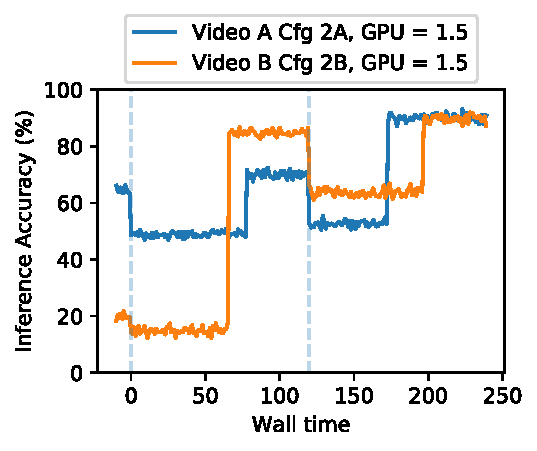
\includegraphics[width=\linewidth]{ekya/figures/motivation/Scheduler/schedmot_multiwindow_optimal_cfgs.pdf}
%    \caption{Optimal cfgs for retraining window}
%    \label{fig:schedmot-optimalcfg}
%  \end{subfigure}
  ~~
  \begin{subfigure}[t]{0.47\columnwidth}
    \centering
    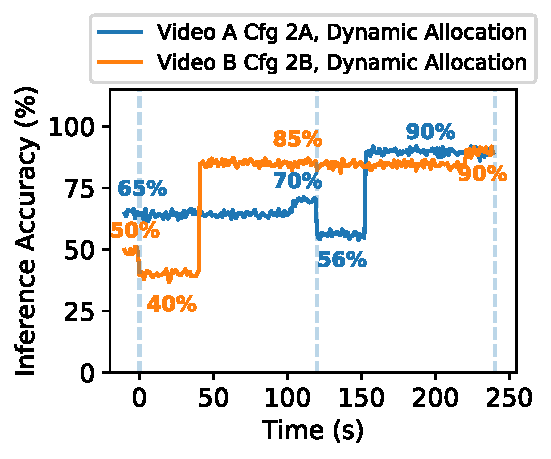
\includegraphics[width=\linewidth]{ekya/figures/motivation/Scheduler/schedmot_multiwindow_prioritization_and_optimal_cfgs.pdf}
    \caption{Accuracy-optimal scheduler}
    \label{fig:schedmot-prioritization}
  \end{subfigure}
  ~~
  \caption{Resource allocations (top) and inference accuracies (bottom) over time for two retraining windows (each of $120$s). The left figures show a uniform scheduler which evenly splits the $3$ GPUs, and picks configurations resulting in the most accurate models. The right figures show the accuracy-optimized scheduler that prioritizes resources and optimizes for inference accuracy averaged over the retraining window ($73\%$ compared to the uniform scheduler's $56\%$). The accuracy-optimized scheduler also ensures that inference accuracy never drops below a minimum (set to $40\%$ in this example, denoted as $a_\text{MIN}$). %\ga{Needs better colors.} \ga{Visually align x-axes in Figures 5a, 5c and Figures 5b, 5d.}
  %\ion{The problem I have with this example is that the "optimal" solution in (d) gets lower minima. It is just not clear to me why a better average but a lower min is necessary better than a lower average but a higher min.} 
  %\romil{Make this easier to read by adding text annotations to accuracy when it changes }
  %Resource allocation maps for toy retraining schedules in Figure \ref{fig:schedmot}. (\ref{fig:schedmot-naive}) and (\ref{fig:schedmot-res-optimalcfg}) run a fair scheduler which evenly splits resources between the two cameras. (\ref{fig:schedmot-res-prioritization}) deprioritizes Camera B's inference task due because of its low accuracy, and instead focuses resources on retraining it. On the other hand, Camera A's inference job is already at an high accuracy, thus it deprioritizes it's retraining job until Camera B is retrained.
  }
  \label{fig:schedmot}
\end{figure}


\noindent{\bf Tradeoffs in inference configurations.} %As described in \S\ref{subsec:edge}, inference operations using the DNNs on the live video streams is a key workload on edge servers. 
Inference pipelines also allow for flexibility in their resource demands at the cost of accuracy through configurations to downsize and sample frames \cite{rocket-github}. \revtext{Reducing the resource allocation to inference pipelines increases the processing latency per frame, which then calls for sub-sampling the incoming frames to match the processing rate, that in turn reduces inference accuracy \cite{videostorm}.} 
Prior work has made dramatic advancements in %configurations to control the resource usage of inference operations by downsizing frames to lower resolutions and sampling of frames, as well as 
profilers that efficiently obtain the resource-accuracy relationship for {\em inference configurations} \cite{chameleon}. We use these efficient inference profilers in our solution, and also to ensure that the inference pipelines keep up with analyzing the live video streams. % with their currently allocated resources. %We use these profilers in our solution to ensure that inference pipelines continue to keep up with analyzing the live video streams with their currently allocated resources.% even as they produce outputs of lower accuracy during the retraining.
%- \romil{Talk about the phenomenon of decrease in accuracy when inference is resource-starved. Any sources? Chameleon?}


%Since each model has multiple resource-accuracy configurations to pick from (\cref{fig:resource-profiles}), the scheduler must be careful while doing this in a time-bound setting. A naive approach would be to pick the hyperparameters which yield the best accuracy at completion, but the time-sensitive nature of retraining jobs requires the scheduler to also consider the resource-cost of each model.



%\subsection{The Inference Accuracy-over-time Metric.}
%While retraining improves inference accuracy at completion, but also reduces the inference accuracy while it is running because inference resources are diverted to retraining. To capture this tradeoff, we use the inference accuracy over time metric, which is defined as the mean accuracy of the inference job over a retraining window.
%\romil{Still need to explain WHY this metric and what's a retraining window.}


% Hyperparameter table


\subsection{Illustrative scheduling example}
\label{subsec:motivation-sched-example}


We use an example with $3$ GPUs and two video streams, A and B, to show the considerations in scheduling inference and retraining tasks jointly.
Each retraining uses data samples accumulated since the {\em beginning of} the last retraining (referred to as the ``retraining window'').\footnote{Continuous learning targets retraining windows of tens of seconds to few minutes \cite{distribution-20, mullapudi2019}. We use 120 seconds in this example. Our solution is robust to and works with any given window duration for its decisions (See \S{\ref{subsec:eval-understanding}}).} % and we experiment with different durations in \S\ref{sec:evaluation}.} 
%A retraining window consists of model retraining, inference during the retraining with the old model, and inference after the retraining with the retrained model.
% setup and profiles
To simplify the example, we assume the scheduler has knowledge of the resource-accuracy profiles, but these are expensive to get in practice (we describe our efficient solution for profiling in \S\ref{subsec:profiling}).
Table \ref{tab:schedmot-hypparams} shows the retraining configurations ({Cfg1A, Cfg2A, Cgf1B, and Cgf2B}), their respective accuracies after the retraining, and GPU cost.
The scheduler is responsible for selecting configurations and allocating resources for inference and retraining jobs.
%Note that these values vary significantly in different windows because of data drift.
%The retraining jobs for the two video streams, A and B, have two hyperparameter configurations each ({Cfg1A, Cfg2A, and Cgf1B, Cgf2B}), with their respective values of accuracy after the retraining and GPU cost. Note the difference in accuracy values of the same configurations between the two retraining windows. Further, there is also considerable difference among the configurations in their GPU costs for retraining, even when their accuracies are similar (e.g., {Cfg2A} and {Cfg2B} in the second retraining window).% Finally, as we see in the second retraining window, even while camera A's end accuracies (after retraining with Cfg2) is comparable to camera B's accuracies, the latter's current (starting) accuracies are far lower. 





% retraining window, option (a), inference downgrading
%At the start of each retraining window (whose duration is $120$s in our example), resources are allocated to the retraining, even while the inferences continue to execute. The scheduler is also responsible for selecting their configurations (\S\ref{subsec:profiles}). %The choice of configurations provides flexibility in their resource demands. %\ga{Can we stagger the retraining jobs?} 


%Figure \ref{fig:schedmot} shows the effect of resource allocation on the {\em inference} accuracies of the two camera streams --  before the retraining, during the retraining, and after the retraining. The example covers two retraining windows, the choice of configurations for the two video streams, and the resource allocations for retraining and inference (Figure \ref{fig:schedmot-res}).

% fair scheduler
%\noindent{\bf Fair scheduling:} A strawman solution for resource allocation is {\em fair} scheduling \cite{fair-1, fair-2, videostorm}. The fair scheduler evenly splits the GPUs between video streams, and each stream evenly partitions its allocated GPUs for retraining and inference tasks; see Figure \ref{fig:schedmot-res-naive}. The fair scheduler picks those configurations for retraining whose retrained model has the highest accuracy ({Cfg1A, Cfg1B} in Table \ref{tab:schedmot-hypparams} for both windows).
\noindent{\bf {\Fair} scheduling:} Building upon prior work in cluster schedulers \cite{fair-1, fair-2} and video analytics systems \cite{videostorm}, a baseline solution for resource allocation evenly splits the GPUs between video streams, and each stream evenly partitions its allocated GPUs for retraining and inference tasks; see Figure \ref{fig:schedmot-res-naive}. Just like model training systems \cite{vizier,hyperband,pbt}, the baseline always picks the configuration for retraining that results in the highest accuracy ({Cfg1A, Cfg1B} for both windows).


Figure \ref{fig:schedmot-naive} shows the {\em inference} accuracies of the two live streams.
We see that when the retraining tasks take resources away from the inference tasks, the inference accuracy drops significantly ({$65\%$} $\rightarrow$ {$49\%$} for video A and {$50\%$} $\rightarrow$ {$37.5\%$} for video B in Window 1).
%--  before the retraining, during the retraining, and after the retraining -- on two retraining windows. 
%The inference jobs themselves are given lesser resources during the retraining and hence run at configurations with lower accuracy (e.g., by skipping frames). 
%The inference accuracies during the first retraining window (Figure \ref{fig:schedmot-naive}) dropped from {$65\%$} $\rightarrow$ {$49\%$} for video A and {$50\%$} $\rightarrow$ {$37.5\%$} for video B, and a similar drop in the second window. % , there is little time to use the model for inference before the next retraining window. 
%While the retrainings produced a model with higher accuracy, they also took a long time (due to high GPU costs) during which the inference accuracy was lower. 
While the inference accuracy increases \emph{after} retraining, it leaves too little time in the window to reap the benefit of retraining. 
%Averaged over the first retraining window, video A's and B's inference accuracies end up being $54\%$ and $57\%$, even though the configurations themselves ({Cfg1A, Cfg1B}) resulted in retrained models with much higher accuracies of $75\%$ and $90\%$ (Table \ref{tab:schedmot-hypparams}). 
Averaged across both retraining windows, the inference accuracy across the two video streams is only $56\%$ because the gains due to the improved accuracy of the retrained model are undercut by the time taken for retraining (during which inference accuracy suffered).
%As a result, this schedule results in a low mean inference accuracy of 51.82\% when measured over the entire duration of the retraining window (\gaa{120s} in our example).
%\ys{In Fig 4a, how do we ``fairly'' allocate resources after job B training finishes? Maybe we should plot the figures across two columns and vertically align a/c and b/d. }









%\noindent{\bf Retraining-aware fair scheduling:} An alternative to the above fair scheduler is picking hyperparameter configurations with lower GPU demands that train faster ({Cfg2A} and {Cfg2B}; Table \ref{tab:schedmot-hypparams}), and thus allows for inference on the retrained model (with higher accuracy) for a longer duration in the retraining window (see Figure \ref{fig:schedmot-optimalcfg}). This scheme results in the average inference accuracy across the two retraining windows of 62.4\% for the two video streams. However, this scheme still equally partitions resources between the two video streams, allocating 1.5 GPU to each, and further equally allocates it's share to inference and retraining tasks (Figure \ref{fig:schedmot-res-optimalcfg}).  %This is a suboptimal resource allocation, as demonstrated in 

\noindent{\bf Accuracy-optimized scheduling:} %Figures \ref{fig:schedmot-res-prioritization} and \ref{fig:schedmot-prioritization} illustrate an accuracy-optimized scheduler, which takes a holistic view on the multi-dimensional tradeoffs in selecting hyperpareamter configurations and allocating resources.
Figures \ref{fig:schedmot-res-prioritization} and \ref{fig:schedmot-prioritization} illustrate an accuracy-optimized scheduler, which by taking a holistic view on the multi-dimensional tradeoffs, provides an an average inference accuracy of $73\%$. In fact, to match the accuracies, the above {\fair} scheduler would require nearly twice the GPUs (i.e., $6$ GPUs instead of $3$ GPUs). 

This scheduler makes three key improvements. First, the scheduler selects the hyperparameter configurations based on their accuracy improvements \emph{relative} to their GPU cost. It selects lower accuracy options ({Cfg2A/Cfg2B}) instead of the higher accuracy ones ({Cfg1A/Cfg1B}) because these configurations are substantially cheaper (Table \ref{tab:schedmot-hypparams}). 
Second, the scheduler \emph{prioritizes} retraining tasks that yield higher accuracy, so there is more time to reap the benefit from retraining. For example, the scheduler prioritizes B's retraining in Window 1 as its inference accuracy after retraining increases by $35\%$ (compared to $5\%$ for video A).
Third, the scheduler controls the accuracy drops during retraining by balancing the retraining time and the resources taken away from inference. %\footnote{The techniques in our scheduler apply to other optimization metrics too, like max-min of accuracy. Evaluating other metrics is left to future work.}

%The scheduler ensures a minimum inference accuracy (40\% in this example) at all times.


%($1$) Hyperparameter configurations are chosen based on the {\em improvement in accuracy} due to the retraining {\em relative to its GPU cost}. In the first retraining window, {Cfg2} is chosen for video B even though its accuracy is lower than {Cfg1}'s accuracy, because of {Cfg2}'s substantially cheaper resource cost (50 GPU-seconds as opposed to 80; Table \ref{tab:schedmot-hypparams}). 

%\noindent{Resource} allocation is also based on the improvement in accuracy and resource costs. In Figure \ref{fig:schedmot-res-prioritization}, video B's retraining is prioritized in the first retraining window because its accuracy is expected to go up from {$50\%$} to $85\%$ while video A's accuracy improves from {$65\%$} to only $70\%$; see Figure \ref{fig:schedmot-prioritization}. Further, the cost of retraining B ($50$ GPU-seconds) is lower than retraining A ($65$ GPU-seconds). 
%However, camera A's retraining is prioritized in the next window of Figure \ref{fig:schedmot-res-prioritization}.
%Likewise, in the second retraining window, camera A's accuracy has a much higher increase (70\% to 90\%), and thus its training is prioritized (note that camera B's retraining is prioritized in first retraining window). 

%($2$) Resource allocations are {\em jointly decided for inference and training}. In the first retraining window of Figure \ref{fig:schedmot-res-prioritization}, while video B's models are being retrained, resources are taken away from video B's inference (but not from inference of video A). Likewise with video A in the second  window. 

%($3$) Resource allocations and configuration selections optimize the {\em inference accuracy over the retraining window}, i.e., compensating for the reduced inference accuracy during the retraining with the higher accuracy model after the retraining. 

%Taking a holistic view on configuration selection and resource allocation leads to an average inference accuracy of $73\%$ across the two videos and two retraining windows, which is far higher than the earlier {\fair} scheduler ($56\%$). In fact, to match the accuracies, the {\fair} scheduling would require nearly twice the GPU resources (i.e., $6$ GPUs in our example, instead of the currently provisioned $3$ GPUs). 
%We also evaluated a variant of the accuracy-optimized scheduler that chooses configurations as per the principles above but allocates the GPU resources fairly. This lowers the average inference accuracy to $66\%$ (details omitted). Hence, it is crucial to {\em jointly select the configurations and allocate resources}.

%  Aross multiple retraining windows, show:
% \begin{itemize}
%     \item Assume linear degradation of inference
%     \item \textbf{Prioritizing one job over the other based on accuracy estimates}
%     \item \textbf{Picking different hyperparameter within a job}
%     \item \textbf{Accuracy improvement compared to fair sched}
% \end{itemize}
% Give sim examples - fair sched vs best sched

%\subsection{Challenges and Desirable properties}

%The profiles in \S\ref{subsec:profiles} and the example in \S\ref{subsec:motivation-sched-example} highlight the key desirable properties and challenges in developing our solution. ($a$) We need a resource-efficient approach to profiling the retraining jobs to obtain the accuracy of the retrained models and their resource costs, ($b$) Scheduling the resources on the edge should jointly consider both the retraining jobs as well as the inference operations on the live videos, and ($c$) The system should optimize for the accuracy of the inference operations averaged over time, instead of instantaneous values of the inference or accuracy of the retrained models alone.


%!TEX root = main.tex
%!TEX spellcheck = en_US 



\section{{Ekya}: Solution Description}
\label{sec:solution}







% Src: https://docs.google.com/drawings/d/1nBnwhi1agkQVHhFf01fLEV5nnQofWXlroUTv8ZCXxuw/edit?usp=sharing

% We start by formally defining our resource allocation problem (\S\ref{subsec:formulation}). In \S\ref{subsec:thief} and \S\ref{subsec:misc} we explain the design of our scheduling solution {\name} and its different features.

% We first formally define our joint retraining and inference with limited resource problem (\S\ref{subsec:formulation}). 
% We then explain the scheduling algorithm of \name (\S\ref{subsec:thief}) and how it estimates performance gains of various schedules (\S\ref{subsec:profiling}), before highlighting optimizations to address practical issues such as performance estimation errors (\S\ref{subsec:misc}).

%\subsection{Overview}
%\label{subsec:overview}


% overview
Continuous training on limited edge resources requires smartly deciding when to retrain each video stream's model, how much resources to allocate, and what configurations to use. Making these decisions presents two challenges.

First, the decision space of multi-dimensional configurations and resource allocations is computationally more complex than two fundamentally challenging problems of multi-dimensional knapsack and multi-armed bandits (\S\ref{subsec:formulation}). %, thus it is very expensive to explore the space of decisions. 
Hence, we design a {\bf thief scheduler} (\S\ref{subsec:thief}), 
% At the core of {\name} is its resource manager, that we refer to as 
a heuristic that makes the joint retraining-inference scheduling tractable in practice. % by exploring a relatively small yet beneficial fraction of the space of decisions. 
%We first formalize the joint retraining-inference scheduling under limited resource and analyze its complexity (\S\ref{subsec:formulation}). The thief scheduler makes the problem tractable in practice, by exploring a relatively small yet promising fraction of action space.
%, thus significantly reducing the problem complexity.

Second, the scheduler requires the model's exact performance (in resource usage and inference accuracy), but this requires retraining using all the configurations. 
%it is infeasible to know a model's exact performance (in resource usage and inference accuracy) for all retraining configurations, as it requires actual retraining and labeling using all configurations. However, this information is essential for the decision making.
We address this challenge with our {\bf micro-profiler} (\S\ref{subsec:profiling}), which retrains only a few select configurations on 
%which profiles the accuracies of many of retraining configurations by actually using them to retrain the model, but 
a fraction of the data. Figure \ref{fig:sys-arch} presents an overview of {\name}'s components. % with early termination.%, and does so only for a small number of promising configurations.  %and for a small number of training epochs, and then gradually prune the set of promising configurations. 

%To maximize the benefit of retraining, {\name}'s decision making and performance estimation must be fast and resource-efficient. 
%Our techniques (in \S\ref{subsec:thief} and \S\ref{subsec:profiling}) address both challenges. % drastically reduce the cost of decision making and performance estimation. %by at least two orders of magnitude when compared to \gaa{traditional solutions} while reaping the accuracy benefits from retraining. 
% to manage the inference and retraining of multiple videos at an edge server. 
% misc
%As shown, \name also includes practical solutions to a range of challenges in a continuous retraining system (\S\ref{subsec:misc}).



%We build upon the thief scheduler to support checkpointing of models {\em during} retraining (\S\ref{subsubsec:checkpoint}) to provide the inference with more accurate models sooner. 
%{\name} also {\em dynamically reallocates resources} when it detects errors in the resource-accuracy estimations (\S\ref{subsubsec:error-profiles}). %We describe the other factors that impact continuous training in \S\ref{subsec:misc}. 
%Generating the resource-accuracy estimations of the retraining jobs is described in \S\ref{sec:profiling}.


%\begin{table}[t!]
\small
\begin{tabular}{cl}
{\bf Notation} & {\bf Description}\\\hline
$V$ & Set of video cameras\\
$v$ & Single video camera\\\hline
$G$ & Total GPU resources\\
$g^v_R$ & Resources for retraining video stream $v$\\
$g^v_I$ & Resource for inference on video stream $v$\\\hline
$\Gamma_v$ & Set of all configurations for retraining $v$\\
 & (each configuration is referred to as $\gamma_v$)\\
$\Lambda_v$ & Set of all configurations for inference on $v$\\
 & (each configuration is referred to as $\lambda_v$)\\\hline
$a_v$ & Accuracy of inference on video stream $v$\\
$\alpha_v$ & Accuracy of inference over time window\\
$T$ & Retraining window duration\\\hline\\
\end{tabular}
\caption{\label{tab:notations}\small\bf Notations used in {\name}'s description.}
\end{table}

\subsection{\hspace{-0.2cm}Formulation of joint inference-retraining scheduling}
\label{subsec:formulation}
% Setup
We maximize the inference accuracy of all video streams in a retraining window. Table \ref{tab:notations} has the list of relevant notations.
We consider a pool of edge GPUs $G$ (each edge server might have a few GPUs~\cite{azure-ase}) shared by the inference and retraining jobs of a set of video streams $V$, with video $v$($\in V$)'s inference job getting $g^{v}_I$ GPU resources and its training job getting $g^{v}_R$ GPU resources\footnote{\junchen{need to clarify why we only share GPU cycles, not RAM, etc.}}. 
For each video $v \in V$, we denote its inference accuracy $a_v$, which could be improved by retraining.
$\gamma_v$ is the retraining configuration, picked from a pool of \textit{configurations} $\Gamma_v$, to retrain the model of video $v$.
$\lambda_v$ is the inference configuration (e.g., frame sampling rate), picked from an inference resource-accuracy profile $\Lambda_v$ \cite{videostorm, chameleon}, to run the inference job of video $v$.
Note that inference configurations are always chosen such that its resource demand does not exceed the allocation $g^v_I$ for inference.

Given the retraining and inference configurations ($\gamma_v,\lambda_v$) and resource allocations ($g^{v}_R, g^{v}_I$) of a video $v$, its inference accuracy at time $t$ is
$a_v(t, g^v_R, \gamma_v, g^v_I, \lambda_v)$ and inference accuracy measured over the retraining window $T$ can be expressed by 
\[
\alpha_v (T) = \frac{1}{T} \int_{t=0}^{T} a_v(t, g^v_R, \gamma_v, g^v_I, \lambda_v)\ dt
\]


%Edge deployments have one or few edge servers that have multiple video cameras $V$ streaming to them for analytics (\S\ref{subsec:edge}). The analytics on the video streams in $V$ share the same GPU resource pool $G$ (typically, a few GPUs per edge server \cite{azure-ase}). For each video stream $v \in V$, there is a continuous inference job whose inference accuracy is $a_v$. A retraining job is run periodically per video stream which improves $a_v$. The resource pool $G$ must be split across the inference and retraining jobs of all video streams, with video $v$'s inference job getting $g^{v}_I$ GPU resources and its training job getting $g^{v}_R$ GPU resources. Table \ref{tab:notations} has the list of relevant notations.



% Training Profiles. Not going into details on how performance scales with resources..
%Every retraining job of video $v$ has a pool of \textit{configurations} $\Gamma_v$ (\S\ref{subsec:profiles}). Each configuration $\gamma_v \in \Gamma_v$ specifies the hyperparameters and an associated accuracy-resource\_time profile. Increased resource allocation to training grants more resource\_time to the training job, allowing it to achieve a higher accuracy for the same wall\_time. Once a retraining job completes, it updates the inference job with the new model. Similar to the training configurations, the inference job of each camera $c$ has a inference performance profile, which dictates the scaling of the inference accuracy as the inference resource allocation changes.
%\noindent{\bf Configurations:} Every retraining job of video $v$ has a pool of \textit{configurations} $\Gamma_v$. Each configuration $\gamma_v \in \Gamma_v$ specifies the hyperparameters and its accuracy (see \S\ref{subsec:profiles}). Increasing resource allocation to retraining ($g^v_R$) allows it complete faster and update the inference job sooner with the new model.% with higher accuracy. 
%
%The inference job of each video stream $v$ also has a resource-accuracy profile $\Lambda_v$ \cite{videostorm, chameleon}, with each configuration $\lambda_v \in \Lambda_v$ (e.g., frame sampling rate) in the profile specifying the current inference accuracy ($a_v$) as well as the resource {\em demand} to keep up with the processing of the live video stream. %All the inference configurations can keep up with processing the live video stream if its corresponding resource demand is allocated, but their accuracies will vary. % which dictates the scaling of the inference accuracy as the inference resource allocation changes.
%Inference configurations are always chosen such that its resource demand does not exceed the allocation $g^v_I$ for inference.

% Define inference accuracy.
%\noindent{\bf Inference accuracy over time:} 
%The inference accuracy of a video $v$ measured over the retraining window depends on the inference configuration (which in turn depends on its resources allocation $g^v_I$) as well as the inference model (pre-retraining and post-retraining). The accuracy of the model post-retraining depends on the retraining configuration $\gamma_v \in \Gamma_v$ and the GPU allocation to the retraining $g^v_R$. Thus, for a video stream $v$ whose inference accuracy at any point in time is $a_v$, the inference accuracy $\alpha_v$ averaged over time $t=0 \rightarrow T$ is (where $T$ is the retraining window):
%\[
%\alpha_v (T) = \frac{1}{T} \int_{t=0}^{T} a_v(t, g^v_R, \gamma_v, g^v_I, \lambda_v)\ dt
%\]

% Objective - What are the metrics and why
\noindent The joint retraining-inference optimization maximizes the average accuracy over a retraining window across all videos through selecting configurations ($\gamma_v$ and $\lambda_v$) and allocating resource between retraining ($g^{R}_v$) and inference ($g^{I}_v$):
\begin{equation}
    \begin{aligned}
        & \underset{g_{R}^v, g_{I}^v, \gamma_v, \lambda_v}{\text{maximize}}
        %& & \frac{\sum_{v \in V}\alpha_v(T, g_{R}^v, \gamma_v, g_{I}^v, \lambda_v)}{|V|} \\
        & & \frac{\sum_{v \in V}\alpha_v(T)}{|V|} \\
        & \text{s.t.}
        & & \sum_{v \in V} g_{R}^v + g_{I}^v \leq G\\
        %&&& a_v(t, g_{R}^v, \gamma_v, g_{I}^v, \lambda_v) \geq a_\text{MIN} \\
        &&& a_v(t) \geq a_\text{MIN}, \forall v \in V, 0 \leq t \leq T 
        %TODO(romilb): Cleanup this min accuracy expression
    \end{aligned}
    \label{eqn:optimization}
\end{equation}
The joint retraining-inference scheduling essentially balances the inference accuracy before retraining finishes and the optimization of long-term accuracy by finishing model retraining as soon as possible.
This fundamentally differs from optimization for only inference accuracy or only training accuracy in two aspects.
Additionally, we allow for the inference accuracy $a_v$ at any point in time to be bounded by a minimum $a_\text{MIN}$ (application-specific bound), so that the inference results remain useful to the application, especially when the model is being retrained.


%As shown in \S\ref{subsec:motivation-sched-example}, optimizing for only the inference accuracy or only the retraining accuracy does not maximize the inference accuracy over the retraining window, $\alpha_v (T)$. % over all cameras $v \in V$. 
%%optimizing for maximum training accuracy is immaterial since the goal is not just to retrain the model, but also use it while it is still useful. Thus the objective is to maximize the mean inference accuracy across all cameras $C$ present in the system by picking the correct configurations and resource allocations, constrained by the size of the resource pool available.
%% https://jcnts.wordpress.com/2009/11/11/formatting-optimization-problems-with-latex/
%%\noindent{\bf Optimization formulation:} 
%
%We seek to maximize the average inference accuracy over the retraining window $T$ (i.e., $\alpha_v(T)$) across all videos $v \in V$ by picking the configurations $\gamma_v$ and $\lambda_v$ for each video stream $v$'s retraining and inference, and allocating the edge's GPU resource $G$ for retraining ($g^{R}_v$) and inference ($g^{I}_v$). Additionally, we allow for the inference accuracy $a_v$ at any point in time to be bounded by a minimum $a_\text{MIN}$ (application-specific bound), so that the inference results remain useful to the application.

% computationally intractable
\mypara{Complexity analysis}
The complexity of the above optimization is combinatorial in the number of configurations and cameras. As a result, we proceed to devise an efficient scheduling heuristic.% that provides good results in practice.
\junchen{Kevin, the complexity discussion can be here}






\subsection{Formulation of joint inference and retraining}
\label{subsec:formulation}

The problem of joint inference and retraining aims to maximize overall inference accuracy for all video streams $\mathcal{V}$ in a retraining window ${T}$ with duration $\lVert T \rVert$. 
All work must be done in $\mathcal{G}$ GPUs.
Thus, the total compute capability is $\mathcal{G}\lVert T \rVert$ GPU-time. Without loss of generality, let $\delta$ be the smallest granularity of GPU allocation.  %(e.g., if $\delta = 1\%$ of GPU, $150\delta =$ 1.5 GPU). Let $\Theta$ be the set of all possible GPU allocations $\Theta = \{0, 1, ..., \frac{\mathcal{G}}{\delta}\}$.
Each video $v \in V$ has a set of \emph{retraining} configurations $\Gamma$
and a set of \emph{inference} configurations $\Lambda$ (\S\ref{subsec:profiles}).
Table \ref{tab:notations} (\S{\ref{appendix:scheduler}}) lists the notations. 



\noindent\textbf{Decisions.} For each video $v\in\mathcal{V}$ in a window $T$, we decide: (1) the retraining configuration $\gamma\in\Gamma$ ($\gamma = \emptyset$ means no retraining); (2) the inference configuration $\lambda\in\Lambda$; and (3) how many GPUs (in multiples of $\delta$) % (in terms of GPU resource units $\delta$)
to allocate for retraining ($\mathcal{R}$) %\in\Theta$) 
and inference ($\mathcal{I}$). %\in\Theta$). 
We use binary variables $\phi_{v\gamma\lambda\mathcal{R}\mathcal{I}}\in\{0,1\}$ to denote these decisions (see Table \ref{tab:notations} \S{\ref{appendix:scheduler}} for the definition). 
These decisions require $C_T(v, \gamma, \lambda)$ GPU-time and yields overall accuracy of $A_T(v, \gamma, \lambda, \mathcal{R}, \mathcal{I})$. $A_T(v, \gamma, \lambda, \mathcal{R}, \mathcal{I})$ is averaged across the window $T$ (\S\ref{subsec:motivation-sched-example}), and the above decisions determine the inference accuracy at {\em each point in time}.
%Specifically, let $a_t(v, \gamma, \lambda, \mathcal{R}, \mathcal{I})$ be the inference accuracy for video $v$ at a point in time $t$, % given retraining configuration $\gamma$, inference configuration $\lambda$, $\mathcal{R}\delta$ GPUs for retraining, and $\mathcal{I}\delta$ GPUs for inference, we have:
%\[
%\ A_T(v, \gamma, \lambda, \mathcal{R}, \mathcal{I}) = 
%\frac{1}{\lVert T \rVert} \int_{t=0}^{\lVert T \rVert} a_t(v, \gamma, \lambda, \mathcal{R}, \mathcal{I})\ dt
%\]


%At each retraining window $t \in \mathcal{T}$, the system maintains a set of DNN instances $M_{v}^t$ for video $v$, where each $m_{v\gamma}^t \in M_{v}^t$ denotes a DNN instance that is trained based on configuration $\gamma$. Each DNN $m_{v\gamma}^0 \in M_{v}^0$ is pretrained with offline video data. 
%The system can optionally retrain $m_{v\gamma}^t$ into $\hat{m}_{v\gamma}^t$ with training configuration $\gamma$ and the video data of $v$ at $t$, and the retraining cost is $C^R(v, t, \gamma)$.

%The system must pick a DNN $m_{v\gamma}^t$ or $\hat{m}_{v\gamma}^t$ and an inference configuration $\lambda \in \Lambda$ to run inference for video $v$ at $t$.
%The inference cost of such a decision is $C^I(v, t, \gamma, \lambda$), and the inference accuracy is $A(v, t, m, \lambda)$ where $m$ is the chosen DNN. 
%We use binary variables $r_{vt\gamma g}$ and $i_{vt\gamma \lambda g}$ to indicate the decisions made by the system (see Table \ref{tab:notations} for their definitions).

\noindent\textbf{Optimization.} Maximize the inference accuracy averaged across all videos in a retraining window within the GPU limit. 

{\small
\vspace{-12pt}
\begin{equation}
    \begin{aligned}
    %\footnotesize
       & \underset{\phi_{v\gamma\lambda\mathcal{R}\mathcal{I}}}{\arg\max}
         \frac{1}{\lVert \mathcal{V} \rVert}
         \sum_{\substack{\forall v\in\mathcal{V}, 
                        \forall \gamma\in\Gamma,
                        \forall \lambda\in\Lambda,\\
                        \forall \mathcal{R}, \forall \mathcal{I} \in \{0, 1, ..., \frac{\mathcal{G}}{\delta}\} %\in \Theta,
                        %\forall \mathcal{I} \in \Theta
                        }}
          \phi_{v\gamma\lambda\mathcal{R}\mathcal{I}} \cdot
          A_T(v, \gamma, \lambda, \mathcal{R}, \mathcal{I})\\
       & \text{subject to}\\
       & 1. \sum_{\substack{\forall v\in\mathcal{V}, 
                        \forall \gamma\in\Gamma,
                        \forall \lambda\in\Lambda,\\
                        \forall \mathcal{R}, \forall \mathcal{I}}}
                        \phi_{v\gamma\lambda\mathcal{R}\mathcal{I}} \cdot
                        C_T(v, \gamma, \lambda)
                        \leq \mathcal{G}\lVert T \rVert \\
      & 2. \sum_{\substack{\forall v\in\mathcal{V},
                        \forall \gamma\in\Gamma,
                        \forall \lambda\in\Lambda,\\
                        \forall \mathcal{R}, \forall \mathcal{I}}}
                           \phi_{v\gamma\lambda\mathcal{R}\mathcal{I}} \cdot
                           (\mathcal{R} + \mathcal{I})
                        \leq \frac{\mathcal{G}}{\delta} \\
      & 3. \sum_{\substack{\forall \gamma\in\Gamma, 
                           \forall \lambda\in\Lambda,\\ 
                           \forall \mathcal{R}, %\in \Theta,
                           \forall \mathcal{I}}} %\in \Theta}}
           \phi_{v\gamma\lambda\mathcal{R}\mathcal{I}} \leq 1, 
           \forall v\in\mathcal{V}
    \end{aligned}
    \label{eqn:optimization}
\end{equation}
}%

The first constraint ensures that the GPU allocation does not exceed the available GPU-time $\mathcal{G}\lVert T \rVert$ in the retraining window. The second constraint limits the {\em instantaneous}  allocation (in multiples of $\delta$) to never exceed the available GPUs. 
%The third constraint ensures that the system can only pick at most one retraining configuration/allocation and one inference configuration/allocation for each video $v$.
The third constraint ensures that at most one configuration is picked for retraining and inference each for a video $v$.





% https://docs.google.com/drawings/d/1nBnwhi1agkQVHhFf01fLEV5nnQofWXlroUTv8ZCXxuw/edit?usp=sharing
%\begin{figure*}[t!]
%    \centering
%    \includegraphics[width=0.85\linewidth]{ekya/figures/Solution/"Ekya System Architecture Arch".pdf}
%    \caption{{\name} System Architecture. \ga{Make it a one-column figure.}}
%    \label{fig:sys-arch}
%\end{figure*}

% % rest of the section
% \subsection{Solution Overview}
% \label{subsec:overview}

% Figure \ref{fig:sys-arch} presents an overview of {\name} to manage the inference and retraining of videos at an edge server. At the core of {\name} is its resource manager, that we refer to as ``thief'' scheduler, which is a greedy scheduling heuristic (\S\ref{subsec:thief}). We build upon the thief scheduler to support checkpointing of models {\em during} retraining (\S\ref{subsubsec:checkpoint}) to provide the inference with more accurate models sooner. {\name} also {\em dynamically reallocates resources} when it detects errors in the resource-accuracy estimations (\S\ref{subsubsec:error-profiles}). %We describe the other factors that impact continuous training in \S\ref{subsec:misc}. 
% Generating the resource-accuracy estimations of the retraining jobs is described in \S\ref{sec:profiling}.
%\revtext{This optimization problem can be expressed as a multi-dimensional binary knapsack problem while the uncertainty of $A_T(v, \gamma, \lambda, \mathcal{R}, \mathcal{I})$ can be modelled as multi-armed bandits (MAB) problem. A detailed complexity analysis is presented in \S\ref{complexity-analysis}.}
Our analysis in \S\ref{complexity-analysis} shows that the above optimization problem is {\em harder} than the multi-dimensional binary knapsack problem and modeling the uncertainty of $A_T(v, \gamma, \lambda, \mathcal{R}, \mathcal{I})$ is more challenging than the multi-armed bandit problem.
%\ga{Summarize the complexity analysis.}


\begin{figure}[ht]
    \centering
    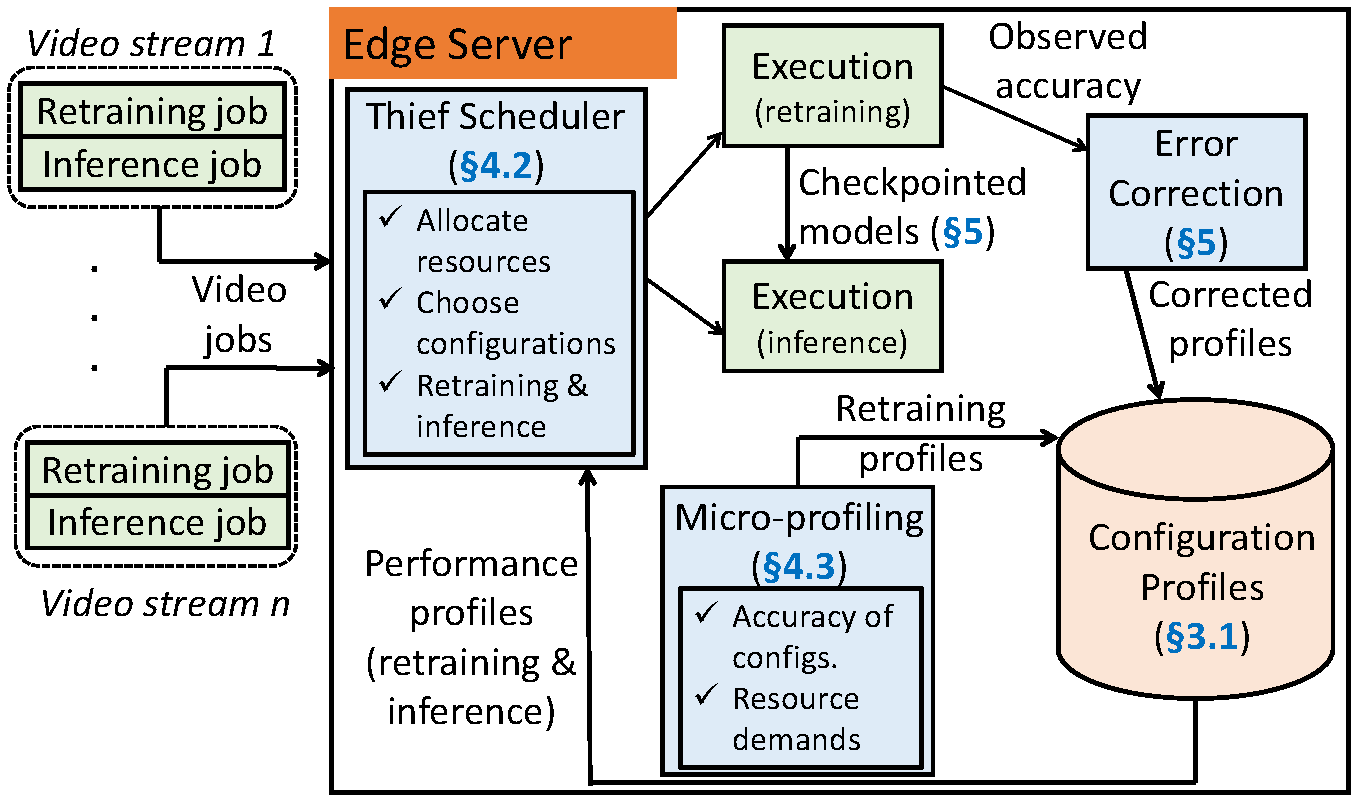
\includegraphics[width=.85\columnwidth]{ekya/figures/overview_cropped.pdf}
    \caption{{\name}'s components and their interactions. }%\ga{Update with the right section numbers.}}
    \label{fig:sys-arch}
\end{figure}

\subsection{Thief Scheduler}
\label{subsec:thief}




%The computational intractability of the formulation in \S\ref{subsec:formulation} stems primarily from jointly allocating resources and picking configurations. In this section, we decouple the two and develop an efficient and iterative heuristic (Algorithm \ref{algo:thief_sched}). 
Our scheduling heuristic makes the scheduling problem tractable by decoupling resource allocation (i.e., $\mathcal{R}$ and $\mathcal{I}$) and configuration selection (i.e., $\gamma$ and $\lambda$) (Algorithm \ref{algo:thief_sched}). %It iteratively allocates resources to all inference and retraining jobs and picks inference/retraining configurations within the limit of the allocated resource. 
%We present the heuristic and then explain the key assumptions and relaxations that it is built upon. 
%\textbf{Challenge:} Equation \ref{eqn:optimization} requires that both the resource allocation and the configurations must be picked jointly. One influences the other, thus we present an iterative algorithm \ref{algo:thief_sched} which tries to converge on the optimal (?) combination.
We refer to {\name}'s scheduler as the ``thief'' scheduler and it iterates among all inference and retraining jobs as follows.% and picks inference/retraining configurations within the limit of the allocated resource. %configuration selection as follows. 
%\begin{packeditemize}

%\item 
{\bf (1)} It starts with a fair allocation for all video streams $v \in V$ (line 2 in Algorithm \ref{algo:thief_sched}). 
In each step, it iterates over all the inference and retraining jobs of each video stream (lines 5-6), and {\em steals} a tiny quantum $\Delta$ of resources (in multiples of $\delta$; see Table \ref{tab:notations}, \S\ref{appendix:scheduler}) from each of the other jobs (lines 10-11).

%\item 
{\bf (2)} With the new resource allocations ({\small temp\_alloc[]}), it then selects configurations for the jobs using the {\sf\footnotesize PickConfigs} method (line 14 and Algorithm \ref{algo:pickconfigs}, \S{\ref{appendix:scheduler}}) that iterates over all the configurations for inference and retraining for each video stream.  
For inference jobs, among all the configurations whose accuracy is $\geq a_\text{MIN}$, {\sf\footnotesize PickConfigs} picks the configuration with the highest accuracy that can keep up with the inference of the live video stream given current allocation (line 3-4, Algorithm \ref{algo:pickconfigs}, \S{\ref{appendix:scheduler}}).  

For retraining jobs, {\sf\footnotesize PickConfigs} picks the configuration that maximizes the accuracy $A_T(v, \gamma, \lambda, \mathcal{R}, \mathcal{I})$ over the retraining window for each video $v$ (lines 6-12, Algorithm \ref{algo:pickconfigs}, \S{\ref{appendix:scheduler}}). {\sf\footnotesize EstimateAccuracy} (line 7, Algorithm \ref{algo:pickconfigs}, \S\ref{appendix:scheduler}) aggregates the instantaneous accuracies over the retraining window for a given pair of inference configuration (chosen above) and retraining configuration. {\name}'s micro-profiler (\S\ref{subsec:profiling}) provides the estimate of the accuracy and the time to retrain for a retraining configuration when $100\%$ of GPU is allocated, and {\sf\footnotesize EstimateAccuracy} proportionately scales the GPU-time for the current allocation (in {\small temp\_alloc[]}) and training data size. In doing so, it avoids configurations whose retraining durations exceed $\lVert T \rVert$ with the current allocation (first constraint in Eq. \ref{eqn:optimization}). %, while ensuring the total compute cost does not exceed the total GPU time. 
%\S\ref{subsec:profiling} explains how we estimate the accuracy of retraining and \gaa{time to retrain} with each configuration. %\footnote{\S\ref{subsec:profiling} estimates the time to retrain when $100\%$ of the GPU is allocated to the retraining, and we linearly estimate the time taken to retrain for any given allocation and training data size inside {\sf PickConfigurations}.}
%We proportionately scale the GPU-time for any given allocation and training data size in {\sf\footnotesize PickConfigs}. \S\ref{subsec:profiling} explains how we estimate the accuracy of retraining and the time to retrain when $100\%$ of the GPU is allocated. 

% {\sf\small PickConfigurations} only checks the Pareto boundary of configurations (Figure \ref{fig:resource-profiles}). 

%\item
{\bf (3)} After reassigning the configurations, {\name} uses the estimated average inference accuracy (accuracy\_avg) over the retraining window (line 14 in Algorithm \ref{algo:thief_sched}) and keeps the new allocations only if it improves up on the accuracy from prior to stealing the resources (line 15 in Algorithm \ref{algo:thief_sched}).

%using {\sf\small Estim} (line 14). 
% the accuracy after stealing resources is higher than the accuracy prior to the stealing (line 14).
%\end{packeditemize}
%steals an additional quantum $\delta$ for the {\small thief\_job} 
%The performance estimation module ({\sf\small Estim}) can produce the $\alpha_v(T)$ for all the video streams $v \in V$ with any given configuration and resource allocation, and we will explain it in next in \S\ref{subsec:profiling}.


The thief scheduler repeats the process till the accuracy stops increasing (lines 15-20 in Algorithm \ref{algo:thief_sched}) and until all the jobs have played the ``thief''. 
Algorithm~\ref{algo:thief_sched} is invoked at the beginning of each retraining window, as well as on the completion of every training job during the window.% to reallocate resources to the other training and inference jobs.

% \begin{algorithm}
%  \KwData{Configuration profiles $\Gamma_v$ and $\Lambda_v$ and resource allocations $g^{c}_R$ and $g^{c}_I$ for video $v$}
%  \KwResult{The optimal configurations $\gamma^{opt}_{v}$ and  $\lambda^{opt}_{v}$}
%  
%  best\_accuracy = 0\;
%  \For{$\lambda_v$ in $\Lambda_v$}{
%     \For{$\gamma_v$ in $\Gamma_v$}{
%          accuracy = simulator([$\lambda_v$, $\gamma_v$], [$g^{c}_R$, $g^{c}_I$])\;
%         \If{accuracy > best\_accuracy}{
%             $\lambda^{opt}_{v}$, $\gamma^{opt}_{v}$ = $\lambda_v$, $\gamma_v$\;
%             best\_accuracy = accuracy\;
%         }
%     }
%  }
% 
% return $\lambda^{opt}_{v}$, $\gamma^{opt}_{v}$\;
% \caption{ConfigurationPickingRoutine}
% \label{algo:config_pick}
%\end{algorithm}

\begin{algorithm}[t]
\small
\KwData{Training ($\Gamma$) and inference ($\Lambda$) configurations}
\KwResult{GPU allocations $\mathcal{R}$ and $\mathcal{I}$, chosen configurations ($\gamma \in \Gamma$, $\lambda \in \Lambda$) $\forall v \in V$}% for the period T.}
 
 % Run in a loop to do iterations of configuration selection and resource allocation
all\_jobs[] = Union of inference and training jobs of videos $V$\;
\tcc{Initialize with fair allocation}
 best\_alloc[] = fair\_allocation(all\_jobs)\; 
% \For{iteration in iteration\_count}{
     % Perform SCO - Single camera optimization which picks the best hyperparameters.
%     \For{v in V}{
%        v.training\_config = {\sf\footnotesize PickConfigurations}(v, curr\_alloc[v]) \;
%     }
 best\_configs[], best\_accuracy\_avg =  {\sf\footnotesize PickConfigs}(best\_alloc)\;
     % Perform thief resource stealing
     \tcc{Thief resource stealing}
%     best\_accuracy\_avg = 0\;
     \For{\text{\em thief\_job} in \text{\em all\_jobs[]}}{
        \For{\text{\em victim\_job} in \text{\em all\_jobs[]}}{
            \lIf{\text{\em thief\_job} == \text{\em victim\_job}} {\bf continue}
            temp\_alloc[] $\leftarrow$ best\_alloc[]\;
            \While{true}{
                \tcc{$\Delta$ is the increment of stealing}
                temp\_alloc[victim\_job] $-$= $\Delta$\;
                temp\_alloc[thief\_job] $+$= $\Delta$\;
                \lIf{{\em temp\_alloc[victim\_job]} < {\em 0}}{
                    \bf break
                }
                \tcc{Calculate accuracy over retraining window and pick configurations.}temp\_configs[], accuracy\_avg = {\sf\footnotesize PickConfigs}(temp\_alloc[])\;
                %\tcc{Calculate accuracy over retraining window and pick configurations.}%accuracy\_$\alpha$ = {\sf\footnotesize Estim}(temp\_configs[], temp\_alloc[])\;
                \If{{\em accuracy\_avg} > {\em best\_accuracy\_avg}}{
                    best\_alloc[] = temp\_alloc[]\;
                    best\_accuracy\_avg = accuracy\_avg\;
                    best\_configs[] = temp\_configs[];
                }
                \Else{\bf break\;}
            }
        }
     }
% }
 {\bf return} {best\_alloc[], best\_configs[]}\;
 
 \caption{Thief Scheduler.
 %\junchen{it's going through all the users, rather than iterative algorithm.. may need a better structure}
 %\romil{Explain estim in function call.}
 }
 \label{algo:thief_sched}
\end{algorithm}










%% PickConfigurations
% For the given allocation, finds the best configuration and returns the accuracy gotten by the best configuration and given resource allocation.

\begin{algorithm}[t]
\small
 \KwData{Resource allocations in {temp\_alloc[]}, configurations ($\Gamma$ and $\Lambda$), retraining window $T$, videos $V$}
 \KwResult{Chosen configs $\forall v \in V$, %for the given $\mathcal{R}^\prime$ and $\mathcal{I}^\prime$, 
 average accuracy over $T$}
 
     chosen\_accuracies[] $\leftarrow$\{\}; chosen\_configs[] $\leftarrow$\{\}\;
     \For{\text{\em v} in $V$\text{\em []}}{
        %\tcc{Pick highest accuracy inference cfg}
        infer\_config\_pool[] = $\Lambda$.{\bf where}(\text{resource\_cost} < temp\_alloc[v.inference\_job] \&\& accuracy $\geq a_\text{MIN}$ )\;
        % Add alpha min filter in cfg_pool
        infer\_config = {\bf max}(infer\_config\_pool, {\bf key}=accuracy)\;
        %\tcc{Pick training configuration}
        best\_accuracy = 0\;
        % best\_training\_cfg = None\;
        \For{\text{\em train\_config} in \text{\em $\Gamma$}}{
            \tcc{Estimate accuracy of inference/training config pair over retraining window} % Done using profiles.
            accuracy = {\sf\footnotesize EstimateAccuracy}(train\_config, infer\_config, temp\_alloc[v.training\_job], $T$)\;
            \If{\text{\em accuracy} > \text{\em best\_accuracy}} {
                best\_accuracy = accuracy\;
                best\_train\_config = train\_config\;
            }
        }
        chosen\_accuracies[v] = best\_accuracy\;
        chosen\_configs[v] = \{infer\_config, best\_train\_config\}\;
     }
    {\bf return} chosen\_configs[], {\bf mean}(chosen\_accuracies[])\;
 
 \caption{\bf\small PickConfigs}
 \label{algo:pickconfigs}
\end{algorithm}

%{\name}'s scheduler starts with a {\em fair} resource allocation for all video streams $v \in V$; for any given resource allocation (of a retraining or inference job), it picks the configuration with the highest accuracy but whose resource demand is less than the allocation. % which maximize inference accuracy for this period. The configurations are picked by the configuration picking routine (\cref{algo:hyperparam_pick}), which uses the simulator $S$ to exhaustively evaluate all training configurations $\gamma_v \in \Gamma_v$ and inference configurations $\lambda_v \in \Lambda_v$ for all video streams $v \in V$.

%After picking the configurations for the given fair resource allocation, the thief allocator iterates over every job, steals a tiny quantum of resource from the remaining jobs and evaluates the accuracy this resource allocation with the simulator $S$. If the accuracy increases, it tries stealing more resources till accuracy stops increasing. It then moves to the next job and repeats till all jobs have played the "thief" and arrived at the maximum pareto accuracy. Once this is done, the thief scheduler re-evaluates the hyperparameter configurations with the algorithm to verify if the current selection is optimal for the new resource allocation. If it is, the algorithm terminates. Else, new hyperparameters are selected and the process is repeated.



\mypara{Design rationale} 
We call out the key aspects that makes the scheduler's decision efficient by pruning the search space. %improves its efficiency while potentially introducing sub-optimality to its decisions.
%starting sequence of jobs
%\item {\em Iterating through the jobs only once:} The thief scheduler orders the jobs ({\sf\small all\_jobs}) in descending order of the expected improvement in accuracy (\ie accuracy after the retraining compared to its current accuracy).  This prioritizes jobs with the most improvement to play the ``thief'' and give them more resource first, while ensuring a bounded computational complexity of the thief scheduler.

\begin{itemize}
%quantum of resource increments
\item {\em Coarse allocations:}
The thief scheduler allocates GPU resources in quantums of $\Delta$. \revtext{Intuitively, $\Delta$ is the step size for allocation used by the scheduler. 
Thus, the final resource allocation from the thief scheduler is within $\Delta$ of the optimal allocation.} 
% This makes the thief scheduler arrive at a resource allocation within $\Delta$ of the optimal allocation.} 
We empirically pick a $\Delta$ that is coarse yet accurate enough in practice, while being mindful of modern GPUs\cite{nvidia-mps}; see \S\ref{subsec:eval-understanding}. %We analyze the sensitivity of $\Delta$ in \S\ref{subsec:eval-understanding}. 
Algorithm \ref{algo:thief_sched} ensures that the total allocation is within the limit (second constraint in Eq~\ref{eqn:optimization}). %The smaller the $\Delta$ the closer to optimal is our allocation, but also inefficient to compute. The quantum $\Delta$ is an experimental parameter whose sensitivity we vary in \S\ref{subsec:sensitivity-eval}.

%starting resource allocations
%\item {\em Starting with a fair resource allocations:}As the decision space for GPU resource allocation ($\mathcal{R}$ and $\mathcal{I}$ $\forall v \in \mathcal{V}$) is very large, we start our exploration with the fair allocation. While other initial allocations can also be used, we seek to improve upon the baseline of fair allocations. 

%temporal switch only on job completions
\item {\em Reallocating resources only when a retraining job completes:}
% , but otherwise the thief scheduler does not temporally vary the allocations among running jobs. 
Although one can reallocate GPU resource among jobs at finer temporal granularity (\eg whenever a retraining job has reached a high accuracy), we empirically find that the gains from such complexity is marginal. %further optimizations does not commensurate the added system complexity.
%That said, \name periodically checkpoints the model so that inference can get the up-to-date accuracy from retraining.
% we partially mitigate this drawback in \S\ref{subsubsec:checkpoint} by periodically {\em checkpointing} the model during the retraining and reallocating resources after each checkpoint.

\item{\em Pruned configuration list:} 
Our micro-profiler (described next) speeds up the thief scheduler by giving it only the more promising configurations. Thus, the list $\Gamma$ used in Algorithm \ref{algo:thief_sched} is significantly smaller than the exhaustive set.  
\end{itemize}

% {\name}'s scheduler relies on an estimation module for accuracy ({\sf\small Estim}) that estimates the average inference accuracy over time, $\alpha_v(T)$ over all the video streams $v \in V$, given their retraining and inference configurations, and their respective resource allocations. The estimator {\sf\small Estim} calculates the expected time taken to finish the retraining for each video stream $v$, and then combines that with the reduced inference accuracy during the retraining and the improved inference accuracy after the retraining, to calculate $\alpha_v(T) \forall v$. \footnote{{\sf\footnotesize Estim} assumes that the inference configuration after the retraining is back to its old value that was being used prior to the retraining.} 



\subsection{Performance estimation with micro-profiling}
\label{subsec:profiling}

% problem statement
% As shown in Figure \ref{fig:sys-arch} and 
{\name}'s scheduling decisions in \S\ref{subsec:thief} rely on estimations of post-retraining accuracy and resource demand of the retraining configurations. 
Specifically, at the beginning of each retraining window $T$, we need to {\em profile} for each video $v$ and each configuration $\gamma\in\Gamma$, the accuracy after retraining using $\gamma$ and the corresponding time taken to retrain.% computation cost for retraining.

\mypara{Profiling in \name vs. hyperparameter tuning}
While \name's profiling may look similar to hyperparameter tuning (e.g.,~\cite{DBLP:conf/nips/SnoekLA12,DBLP:journals/jmlr/LiJDRT17,hypersched,rubberband}) at first blush, there are two key differences. 
%First, \name needs not only the performance estimates of the single best configuration, but those of a broad set of candidate configurations as input to the joint retraining-inference scheduling. 
First, \name needs the performance estimates of a broad set of candidate configurations for the thief scheduler, not just of the single best configuration, because the best configuration is jointly decided across the many retraining and inference jobs. 
Second, in contrast to hyperparameter tuning which runs separately of the eventual inference/training, \name's profiling must share compute resource with all retraining and inference.% jobs, and thus must be optimized as a whole. 
%One strawman is to leverage \name periodic retraining and predict the performance of configurations based on their history performance, but we have found that this works poorly in practice, since the performance is heavily influenced by the characteristics of the training data, which vary substantially across retraining windows.

%A strawman is to predict the performance of configurations based on their history from prior training runs, but we discovered that this works poorly in practice. %, since the performance is heavily influenced by the characteristics of the training data which vary substantially across retraining windows. 
%In fact, even when we cached and reused models from prior retraining windows with {\em similar} class distributions, the accuracy was still substantially lower due to other difficult to model factors like lighting, occlusion, etc. (see \S\ref{subsec:eval-alternate}). Thus we adopt an {\em online} estimation approach by using the current retraining window's data.

%Predicting the accuracy of retraining a model is challenging because it is dependent on the characteristics of the training data. 
%%The challenge is compounded by the diversity in training configurations. 
%As a result, predicting the accuracy of the retraining configurations based on history are less suited. \footnote{\ga{Provide details and quantify.}}


% so the problem sounds strictly more challenging. 
\mypara{Opportunities} 
\name leverages three empirical observations for efficient profiling of the retraining configurations. 
$(i)$ Resource demands of the configurations are deterministic. Hence, we measure the GPU-time taken to retrain for {\em each epoch} in the current retraining window when $100\%$ of the GPU is allocated to the retraining. \revtext{This GPU-time must then be re-scaled for varying number of epochs, GPU allocations, and training data sizes in Algorithm \ref{algo:thief_sched}. 
For re-scaling number of epochs and training data sizes, we linearly scale the GPU-time. For re-scaling GPU allocations, we use an offline computed profile of the model throughput for different resource allocations to account for sub-linear scaling.
%In our implementation of the algorithm, we linearly scale the GPU-time for any given number of epochs or data size, which closely matches their true GPU-time.
%However, we profile the GPU-time of the trained model architecture (\eg ResNet18) under for various GPU cycles offline, rather than linearly extrapolate.
Our real testbed-based evaluation shows that these rescaling functions works well in practice.
}% \footnote{For the object detection and classification models that we consider, both the computation demands per training epoch and the number of epochs for convergence highly correlate with the size of the training data.}
$(ii)$ Post-retraining accuracy can be roughly estimated by training on a small subset of training data for a handful of epochs.
$(iii)$ The thief scheduler's decisions are not impacted by small errors in the estimations.% (lines 14-17 in Algorithm~\ref{algo:thief_sched}).%, as long as the computation demands of the configurations are precise. 
% We will elaborate them after explaining our design. 

% history-based alternate solution 

%\romil{xx\%} if an initial seed knowledge of the model's training behavior is known. 

% solution's principle - subset of data and configs; result teaser
\mypara{Micro-profiling design} 
The above insights inspired our approach, called {\em micro-profiling}, where 
%We adopt an approach that we call {\em micro-profiling} where we 
for each video, we test the retraining configurations on a {\em small subset} of the retraining data and only for a {\em small number} of epochs (well before models converge). %We then use the observed accuracy of micro-profiling to estimate the post-retraining accuracy using a simple extrapolation.
% Again, the extrapolations of accuracy do not have to be perfect to ensure good scheduling decisions by the thief scheduler.
% \junchen{stopped here}
%While similar schemes are used in hyperparameter tuning~\cite{??} and DNN optimization~\cite{??}, we show that, when used properly, they also enable efficient micro-profiling in \name.
Our micro-profiler is $100\times$ more efficient than exhaustive profiling (of all configurations on the entire training data), while predicting accuracies with an error of $5.8\%$, %\junchen{wow, this sounds surprisingly low!}, 
which is low enough in practice to {\em mostly} ensure that the thief scheduler makes the same decisions as it would with a fully accurate prediction. % good allocations by the thief scheduler (\S\ref{subsec:thief}). % \ga{We should elaborate why the thief scheduler works well with inaccurate profiles.}. 
We use these insights to now explain the techniques that make {\name}'s micro-profiling efficient.


%We simplify the accuracy prediction problem by training each configuration for a short duration on a sub-sample of the data. This micro-profiling process produces an accuracy value for each configuration when trained for a short duration on a subsample of the data. With each configuration's microprofiled accuracy as an input to the training loss curve model from \cite{optimus}, we can produce accuracy estimates for different epochs\romil{Add optimus model here}.we

% subset of data
% \noindent{\em 1) Data sampling:} 
\noindent{\em 1) Training data sampling:}  
{\name}'s micro-profiling works on only a small fraction (say, $5\%-10\%$) of the training data in the retraining window (which is already a subset of all the videos accumulated in the retraining window). While we considered weighted sampling techniques for the micro-profiling, we find that uniform random sampling is the most indicative of the configuration's performance on the full training data, since it preserves all the data distributions and variations. % (in terms of classes, appearances, etc.).
% . We surmise that uniform sampling preserves the biases (in terms of classes, appearances, etc.) that are present in the full training dataset, thus leading to more precise resource-accuracy profiles to provide to the thief scheduler (Figure \ref{fig:sys-arch}). 

% config extrapolation (num. of epochs)
% \noindent{\em 2) Continuous hyperparameters:}
\noindent{\em 2) Early termination:} 
Similar to data sampling, {\name}'s micro-profiling only tests each configuration for a small number (say, 5) of training epochs.
Compared to a full fledged profiling that needs few tens of epochs to converge, such early termination greatly speeds up the micro-profiling process.
% Similar to data sampling, we also extrapolate the accuracy from hyperparameters that are {\em continuous}, e.g., number of epochs in the training. We contrast hyperparameters whose values are on a continuous scale from the others that are discrete (like \gaa{the number of layers to freeze during retraining}). Our \gaa{evaluations in \S\ref{sec:evaluation}} show that the error in extrapolating accuracies of such continuous hyperparameters remains absolutely low.

%\noindent{\em 3) Performance extrapolation:} On its early termination, we obtain the (validation) accuracy of a configuration on the sampled training data, we use a simple linear multiplicative factor, learned from history, to extrapolate the accuracy that would be obtained by retraining with all the data. The use of linear extrapolation is consistent with similar work in this space~\cite{Optimus,ernest}.
%After early termination of the training on the sampled training data, we obtain the (validation) accuracy of each configuration, and use a simple linear multiplicative factor, learned from history, to extrapolate the accuracy that would be obtained by retraining with all the data for larger number of epochs. The use of linear extrapolation is consistent with similar work in this space~\cite{optimus,ernest}. 
After early termination on the sampled training data, we obtain the (validation) accuracy of each configuration at each epoch it was trained. We then fit the accuracy-epoch points to the a non-linear curve model from \cite{optimus} using a non-negative least squares solver~\cite{nnls}. This model is then used to extrapolate the accuracy that would be obtained by retraining with all the data for larger number of epochs. The use of this extrapolation is consistent with similar work in this space~\cite{themis,optimus}. 
%\romil{No, we use the trend from the first 5 epochs to fit a curve to the Optimus model. I can rewrite this.}
% based on the accuracy from retraining on the fraction of the data used in the micro-profiling. Note that the \gaa{resource demands are extrapolated linearly based on the sampling fraction}.

% prune out bad configs
\noindent{\em 3) Pruning bad configurations:} 
Finally, {\name}'s micro-profiling also prunes out those configurations for micro-profiling (and hence, for retraining) that have historically not been useful. These are configurations that are significantly distant from the configurations on the Pareto curve of the resource-accuracy profile (see Figure \ref{fig:darmstadt-profile}), and thus unlikely to be picked by the thief scheduler.
\revtext{To bootstrap pruning, all configurations are evaluated in the first window. After every 2 windows, a fixed fraction of the worst performing configurations are dropped. While first few retraining windows must explore a big space of configurations, the search space size drops exponentially over time.} Avoiding these configurations improves the efficiency of the micro-profiling. 

% golden labels
% \ga{TODO} 
\mypara{Annotating training data} 
For both the micro-profiling as well as the retraining, {\name} acquires labels using a ``golden model'' (\S\ref{subsec:continuous}). This is a high-cost but high-accuracy model trained on a large dataset. %, and the use of such a golden model is consistent with literature in computer vision \cite{incremental-13, mullapudi2019, incremental-15, distribution-20}. 
As explained in \S\ref{sec:background}, the golden model cannot keep up with inference on the live videos and we use it to label only a small subset of the videos for retraining. 
\revtext{The delay of annotating training data with the golden model is accounted by the scheduler as follows: we subtract the data annotation delay from the retraining window and only pass the remaining time of the window to Algorithm \ref{algo:pickconfigs} (\S{\ref{appendix:scheduler}}).}
% \revtext{The cost of annotating training data with the golden model is included in the scheduler by subtracting the label generation time from the size of the retraining window and passing this as the retraining window parameter to the Algorithm \ref{algo:pickconfigs} routine.}
%\junchen{refer to section 2 when golden model labeling is first mentioned?} 
%We use the \gaa{ResNet152} model trained on the MS-COCO dataset as our golden model. While the \gaa{cost of running the golden model is typically a small fraction of the retraining cost (measured to be under $3\%$),} note that the golden model is still significantly more expensive than the compressed edge models and are not conducive for inference on live video streams.

%\junchen{moved reactive error correction from 4.4}

% \subsubsection{Error in accuracy estimates}
% \label{subsubsec:error-profiles}

\eat{
% Traditional hyperparameter tuning
\noindent{\bf Hyperparameter tuning vs. micro-profiling:} We would emphasize that the problem of obtaining the resource-accuracy profiles of the training configurations is different than and unaddressed by traditional hyperparameter tuning techniques\cite{hyperband, asha}. Hyperparameter tuning picks the best performing configurations from a pool of candidate configurations, and thus can be modelled as a multi-armed bandit problem. As a result, multiple configurations are run in parallel and pruned as time progresses. However, our goal in {\name} is to identify the training cost and accuracy for each configuration such that the thief scheduler in \S\ref{subsec:thief} can make a globally optimal decisions on resource management across configurations and video streams. Thus it is necessary to micro-profile each configuration instead of pruning configurations during training. 

\junchen{based on the conversation with Kevin, two differences could be highlighted: (1) we need to profile a broader set of configs since the thief scheduler not only needs the most accurate config. (2) the notion of cost is different: HP tuning treats the profiling costs and actual retraining costs separately, but we need to minimize both. 
however, they are not very strong. (1) makes the problem sounds strictly harder, and (2) still doesn't say why their techniques can't be used as our baseline. in the worst case, we should downplay the microprofiler as opposed to a key tech nugget. }
}
% \romil{Add experiment to justify that golden model outputs are indeed representative of the ground truth}





% profiling problem definition 


% Profiling




%\cref{fig:microprofiling-bench} illustrates the effectiveness of micro-profiling in predicting model accuracy. We microprofile 6 hyperparameter configurations by training them for 5 epochs on 10\% data from a retraining window in the Cityscapes dataset. The accuracies produced by microprofiling are then used to estimate the accuracies if the model was trained without subsampling for 10, 20 and 30 epochs respectively. For comparison, we also train the same configurations for 10, 20 and 30 epochs without subsampling, indicated by the dotted curves. We see that \romil{...}

%\romil{Talk about microprofiling cost/accuracy tradeoff?}





%\begin{figure}
%  \centering
%  \begin{subfigure}[t]{\linewidth}
%    \centering
%    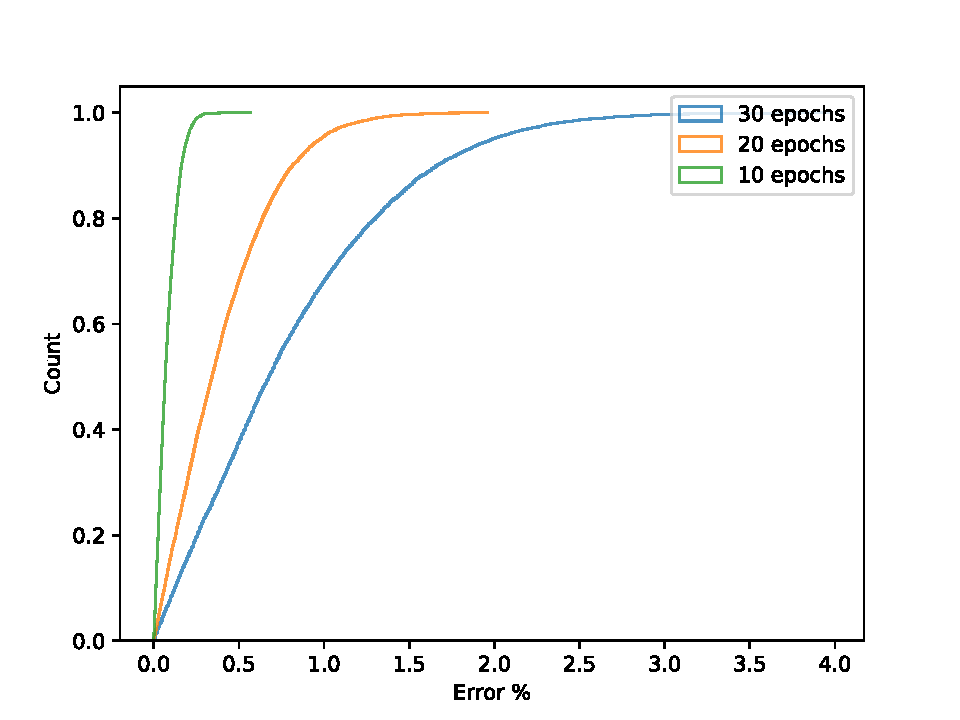
\includegraphics[width=0.9\linewidth]{results/microprofiling_dummy.pdf}
%  \end{subfigure}
%  \caption{Errors in accuracy prediction when using Microprofiling. Accuracy errors are higher when predicting for larger number of epochs, but still within xx\% of the true accuracy.}
%  \label{fig:multicam-cities}
%\end{figure}

 % ADD THIS
%% \section{Ekya Implementation}
\label{sec:system}

% impl overview

% logical integration

% key design choices
% - fine-grained gpu isolation
% - control interface with inference/retraining process
% - efficient support for microprofiling

%\junchen{this is copied from eval}
% We implement a prototype of \name using Python and the Ray framework~ \cite{ray}.

%Next, we describe how \name is integrated with existing libraries of DNN inference/training and the key design choices that optimize \name's efficiency in practice. 

% \subsection{API and integration}
% \label{sec:integration}

%\mypara{Interfaces}
%\junchen{1. what are the input API exposed by \name (sequence of images/frames); 2. what API does \name assume from the GPU library; and from the DNN runtime. 3. and importantly, these APIs are already provided by existing libraries and DNN inference/retraining can be done as is.}
%\name decodes video frames (images) from encoded video streams and feeds the frames to the inference tasks while also accumulating them to be used as input for the model's retraining at the beginning of each retraining window. 
% which are split into retraining tasks.
% Each task is a logical collection of data (images) accumulated in a retraining period. 
\name uses PyTorch \cite{pytorch} for running and training ML models. 
%Note that the training/inference jobs are logically the same as standalone training and inference tasks, so the underlying DNN engine can be seamlessly replaced and improved by better implementation.
%To allocate fractional GPU resources to each job, we need driver-level support from the GPU.
%\name uses Nvidia Multi-Process Service\cite{nvidia-mps} (MPS), which acts as a broker of GPU compute resources by intercepting CUDA calls and re-scheduling them according {\name}'s thief scheduler. 

\mypara{Modularization}
%\junchen{1. Instead of using a single top-down process, \name includes a collection of independent actors, each running the \name's control logic (microprofiling or thief scheduler or a training/inference job. 2. why? scalability? fault tolerance? slightly higher communication cost is tolerable since we operate on timescale of seconds.}
%While \name could be a single process, 
Our implementation uses a collection of logically distributed modules for ease of scale-out to many video streams and resources. 
Each module acts as either the \name scheduler, micro-profiler, or a training/inference job, and is implemented by a long-running ``actor'' in Ray \cite{ray}. 
A benefit of using the actor abstraction is its highly optimized initialization cost and failure recovery. %of training/inference models, thus allowing for % when they must be \gaa{invoked repetitively}, 
%Since an actor can keep a model loaded into GPU memory even when it fails, this allows for 
%quick recovery from failures. 
%\name also uses Ray to handle failures\junchen{Romil, add some details here}. 
% Moreover, this modularization allows Ekya to scale easily to multiple video streams and resources. Finally, actors are able to communicate in a peer-to-peer fashion, which allows training jobs to directly update the inference model when retraining completes.


\mypara{Dynamic reallocation of resources}% GPU isolation
\name reallocates GPU resources between training and inference jobs at timescales that are far more dynamic than required by prior frameworks (where the GPU allocations for jobs are fixed upfront ~\cite{kubernetes, yarn}).  
%There are two approaches to fine-grained GPU isolation for \name: (1) a middle layer, such as the Nvidia MPS~\cite{nvidiamps}, at the GPU driver level can reschedule GPU calls, or (2) dynamically throttling the per-process input load (such as reducing the video sampling rate) to ensure resources are freed up for use by others. 
While a middle layer like Nvidia MPS~\cite{nvidia-mps} provides resource isolation in the GPU by intercepting CUDA calls and re-scheduling them, it also 
%A middle layer like Nvidia MPS 
requires terminating and restarting a process to change its resource allocation. %, whereas throttling the load per-process may have the same effect without restarting the jobs, but Nvidia MPS enforces max-min fairness which does not allow arbitrary GPU partitioning. 
Despite this drawback, \name uses Nvidia MPS due to its practicality, while the restarting costs are largely avoided by the actor-based implementation that keeps DNN model in GPU memory. %\footnote{Currently, \name is limited to managing the GPU compute cycles. Extending {\name} to multiple resources like GPU memory is part of future work.%, and it assumes GPU memory is generally available. Processes today simply fail if they try to allocate more GPU memory than is available. However, 
%It is to be noted that recent work has shown that GPU memory can be virtualized with physical CPU memory \cite{salus, checkmate},and thus out-of-memory situations do not cause catastrophic failure. %In such a situation, GPU memory can be simply handled as an additional resource by \name.
%}
% For simplicity and fast model reloading, we use Nvidia MPS, but future work can consider regulating load as a mechanism to implement resource sharing.  
%\romil{This is not what we really do.. just mentioning it here based on discussion with Junchen.} \romil{Mention the default CUDA max-min fairness work?}


% \mypara{Placement onto GPUs} % GPU isolation
% The resource allocations produced by the thief scheduler are ``continuous'', i.e., it assumes that the fractional resources can be spanned across two discrete GPUs. To avoid the consequent expensive inter-GPU communication, \name first quantizes the allocations to inverse powers of two (\eg 1/2, 1/4, 1/8). This makes the jobs amenable to packing. \name then allocates jobs to GPUs in descending order of demands to reduce fragmentation \cite{tetris}. %, which ensures all jobs fit on the GPUs.


% \mypara{Model checkpointing and reloading}
% \name can improve inference accuracy by checkpointing the model {\em during} retraining and dynamically loading it as the inference model~\cite{tf-checkpoint, torch-checkpoint}.


% Checkpointing can, however, disrupt both the retraining and the inference jobs,
% so {\name} weighs the cost of the disruption (\ie additional delay on retraining and inference) due to checkpointing against its benefits (\ie the more accurate model is available sooner).
% Implementing checkpointing in \name is also made easy by the actor-based programming model that allows for queuing of requests when the actor (model) is unavailable when its new weights are being loaded. 


\mypara{Adapting estimates during retraining}
%{\name} relies on estimates on the expected accuracy from the retraining (to be explained in \S\ref{sec:profiling}), that it uses in Algorithm \ref{algo:thief_sched}. However, when the actual accuracy during the retraining varies from its expected value, {\name} reactively adjusts its allocations. 
When the accuracy during the retraining varies from the expected value from micro-profiling, {\name} reactively adjusts its allocations. 
%The {\em reactive} controller in {\name} (Figure \ref{fig:sys-arch}) monitors the growth in accuracy of the retraining jobs. 
Every few epochs, \name uses the current accuracy of the model being retrained to estimate its eventual accuracy when all the epochs are complete. It updates the expected accuracy in the profile of the retraining ($\Gamma$) with the new value, and then reruns Algorithm \ref{algo:thief_sched} for new resource allocations (but leaves the configuration that is used currently, $\gamma$, to be unchanged). 
%Since the increase in accuracy during the retraining is not always linear with the epochs, {\name} learns the {\em rate} of growth from prior retraining runs. %Further, to improve its estimation, {\name} also uses statistical techniques similar to those in prior work \cite{hyperdrive}.

%Ekya relies on offline profiles for estimating the expected final accuracy and completion time for each job. However, based on the input data, the performance of a model may vary from the expected profile. Ekya must adapt to any such variations.


%Ekya includes a reactive controller which continuously monitors the performance of training jobs and computes their deviation from the expected offline profiles. If the deviation crosses a fixed threshold, the job is immediately checkpointed and terminated and the profile is flagged as unreliable. \romil{Why not continue the job? Perhaps because its a bad use of resources?} If the profile is flagged as unreliable for 2 consecutive retraining windows, then it is allowed to run instead of being terminated, and the profile is updated with the newly observed curve. Thus, erring profiles are continuously updated while minimizing the cost from re-profiling correct profiles.


%\mypara{Batched micro-profiling}
% Microprofiling parallelization
% \junchen{1. why microprofiling needs speedup: while microprofiling reduces the total workload, it is still slow as it needs to test the configs one by one. 2. two optimizations: (a) sampled training data can be fit into memory once and reused; and (b) retraining can be parallelized}
%Micro-profiling, as explained in \S\ref{subsec:profiling}, can still be slow since it requires running multiple independent training jobs to get estimates for each configuration. 
%Since micro-profiling operates on the {\em same} (sub-sampled) data, \name loads the data to GPU memory once and reuses it for micro-profiling the different training configurations. In addition, these micro-profiling jobs can be parallelized and this parallelization also benefits from packing jobs together to maximize utilization~\cite{gandiva}.











% \subsection{Runtime enhancements in retraining window}
% \label{subsec:misc}

% \junchen{todo: 1. add thief scheduler acceleration, 2. maybe move checkpointing to a new implementation section}

% We next present two key enhancements to {\name} to improve its performance {\em during} the retraining of the jobs.

% \subsubsection{Checkpointing models.} 
% \label{subsubsec:checkpoint}





%\subsubsection{Decay factor} The inference accuracy of even the retrained model may {\em decay during the} retraining window because of shifting data distributions. While {\name} supports small retraining windows, we can also incorporate a decay factor (learned from history) in the {\sf\small Estim} module of \S\ref{subsec:thief}. 
%The inference accuracy of a retrained job is expected to decrease as the data distribution shifts over time. This is modeled in the profiles and incorporated in the simulator $S$ of the thief scheduler, which allows the thief scheduler to account for the eventual degradation of a retrainined model when deciding which cameras to prioritize. \romil{Not implemented}

%\noindent{\bf Retraining frequency.} The need for retraining depends on the changes in the data distribution. Some video stream may not require periodic retraining because their distributions may be stationary, while some video streams may change more rapidly, calling for a higher retraining frequency. This information is expected to be captured in the configuration profiles, where subsequent retrainings would demonstrate a lower accuracy gain. This information is directly consumed by thief scheduler which implicitly decides if a camera must be retrained or not by allocating resources. If a camera requires no retraining, the thief allocator will set it's resource allocation to 0. \romil{Add plots on the effects of retraining frequency} \ga{Add this to Section 2.1}

% \subsection{System Implementation}
% \romil{WIP}






%%\section{Accuracy estimation with Microprofiling}
\label{sec:profiling}


% problem statement

% solution's principle - subset of data and configs

% subset of dataw

% config extrapolation (num. of epochs)

% prune out bad configs

% result teaser

% golden labels

% history-based alternate solution 


% profiling problem definition 
As shown in Figure \ref{fig:sys-arch} and explained in \S\ref{sec:solution}, {\name} relies on estimated accuracies of the retraining configurations for its scheduling decisions for each retraining window. Specifically, at the beginning of each retraining window $w$, the thief scheduler requires the estimated accuracy of each configuration $\gamma_v$, denoted as $a_v^{(w,\gamma)}$. The resource demands of the retraining configurations scale well with the size of the training data, and thus they only need to be measured once.

% Profiling
Predicting the accuracy of a fully trained model is challenging because it is dependent on the input data and stochastic training process. The problem is further compounded by the diversity in training configurations, which makes the training process unpredictable. However, as we show below, it is possible to predict the accuracy of a model within \romil{xx\%} if an initial seed knowledge of the model's training behavior is known. 

We simplify the accuracy prediction problem by training each configuration for a short duration on a sub-sample of the data. This micro-profiling process produces an accuracy value for each configuration when trained for a short duration on a subsample of the data. With each configuration's microprofiled accuracy as an input to the training loss curve model from \cite{optimus}, we can produce accuracy estimates for different epochs\romil{Add optimus model here}.

\cref{fig:microprofiling-bench} illustrates the effectiveness of micro-profiling in predicting model accuracy. We microprofile 6 hyperparameter configurations by training them for 5 epochs on 10\% data from a retraining window in the Cityscapes dataset. The accuracies produced by microprofiling are then used to estimate the accuracies if the model was trained without subsampling for 10, 20 and 30 epochs respectively. For comparison, we also train the same configurations for 10, 20 and 30 epochs without subsampling, indicated by the dotted curves. We see that \romil{...}

\romil{Talk about microprofiling cost/accuracy tradeoff?}

% Traditional hyperparameter tuning
Note that this problem different from the traditional hyperparameter tuning\cite{hyperband, asha}. Hyperparameter tuning involves picking the best performing configurations from a pool of candidate configurations, and thus can be modelled as a best-arm identification problem in a multi-armed bandit setting. It is implemented in a similar manner where multiple configurations are run in parallel and pruned as time progresses. However, our goal is not identifying the configuration which would yield the highest accuracy. We need to identify the training cost-accuracy tradeoff for each configuration such that the thief scheduler can make a globally optimal decision across configurations and video streams. Thus it is necessary to micro-profile each configuration instead of pruning configurations at runtime. 

{\bf Training labels.} Note that for the current retraining window as well as for the historical windows, {\name} acquires ``ground-truth'' labels using a golden model -- a high-cost but high-accuracy model pre-trained on a large dataset -- consistent with prior work \cite{incremental-13, mullapudi2019, incremental-15, distribution-20}. In every retraining window, {\name} runs the golden model on the training data to generate labels for retraining. We use the ResNet152 model trained on the MS-COCO dataset as our golden model. The cost of running the golden model is typically small (measured to be under $3\%$ of the retraining cost, as per our experiments).
% \romil{Add experiment to justify that golden model outputs are indeed representative of the ground truth}

\begin{figure}
  \centering
  \begin{subfigure}[t]{\linewidth}
    \centering
    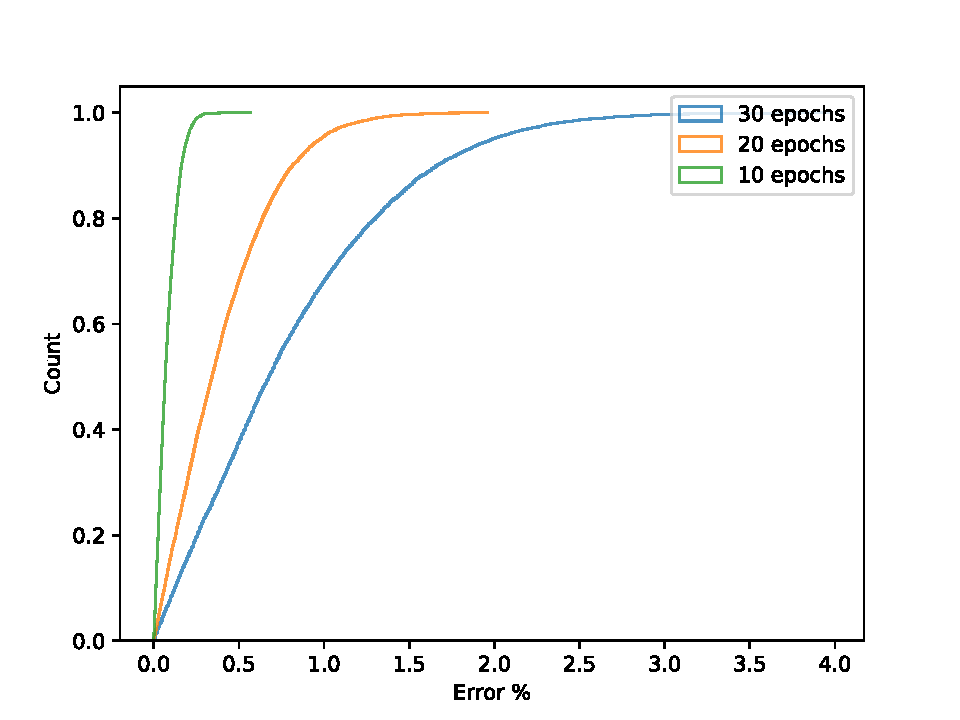
\includegraphics[width=0.9\linewidth]{results/microprofiling_dummy.pdf}
  \end{subfigure}
  \caption{\bf\small Errors in accuracy prediction when using Microprofiling. Accuracy errors are higher when predicting for larger number of epochs, but still within xx\% of the true accuracy.}
  \label{fig:multicam-cities}
\end{figure}


%% 
\begin{figure*}[t]
\begin{subfigure}[b]{0.30\textwidth}
\centering
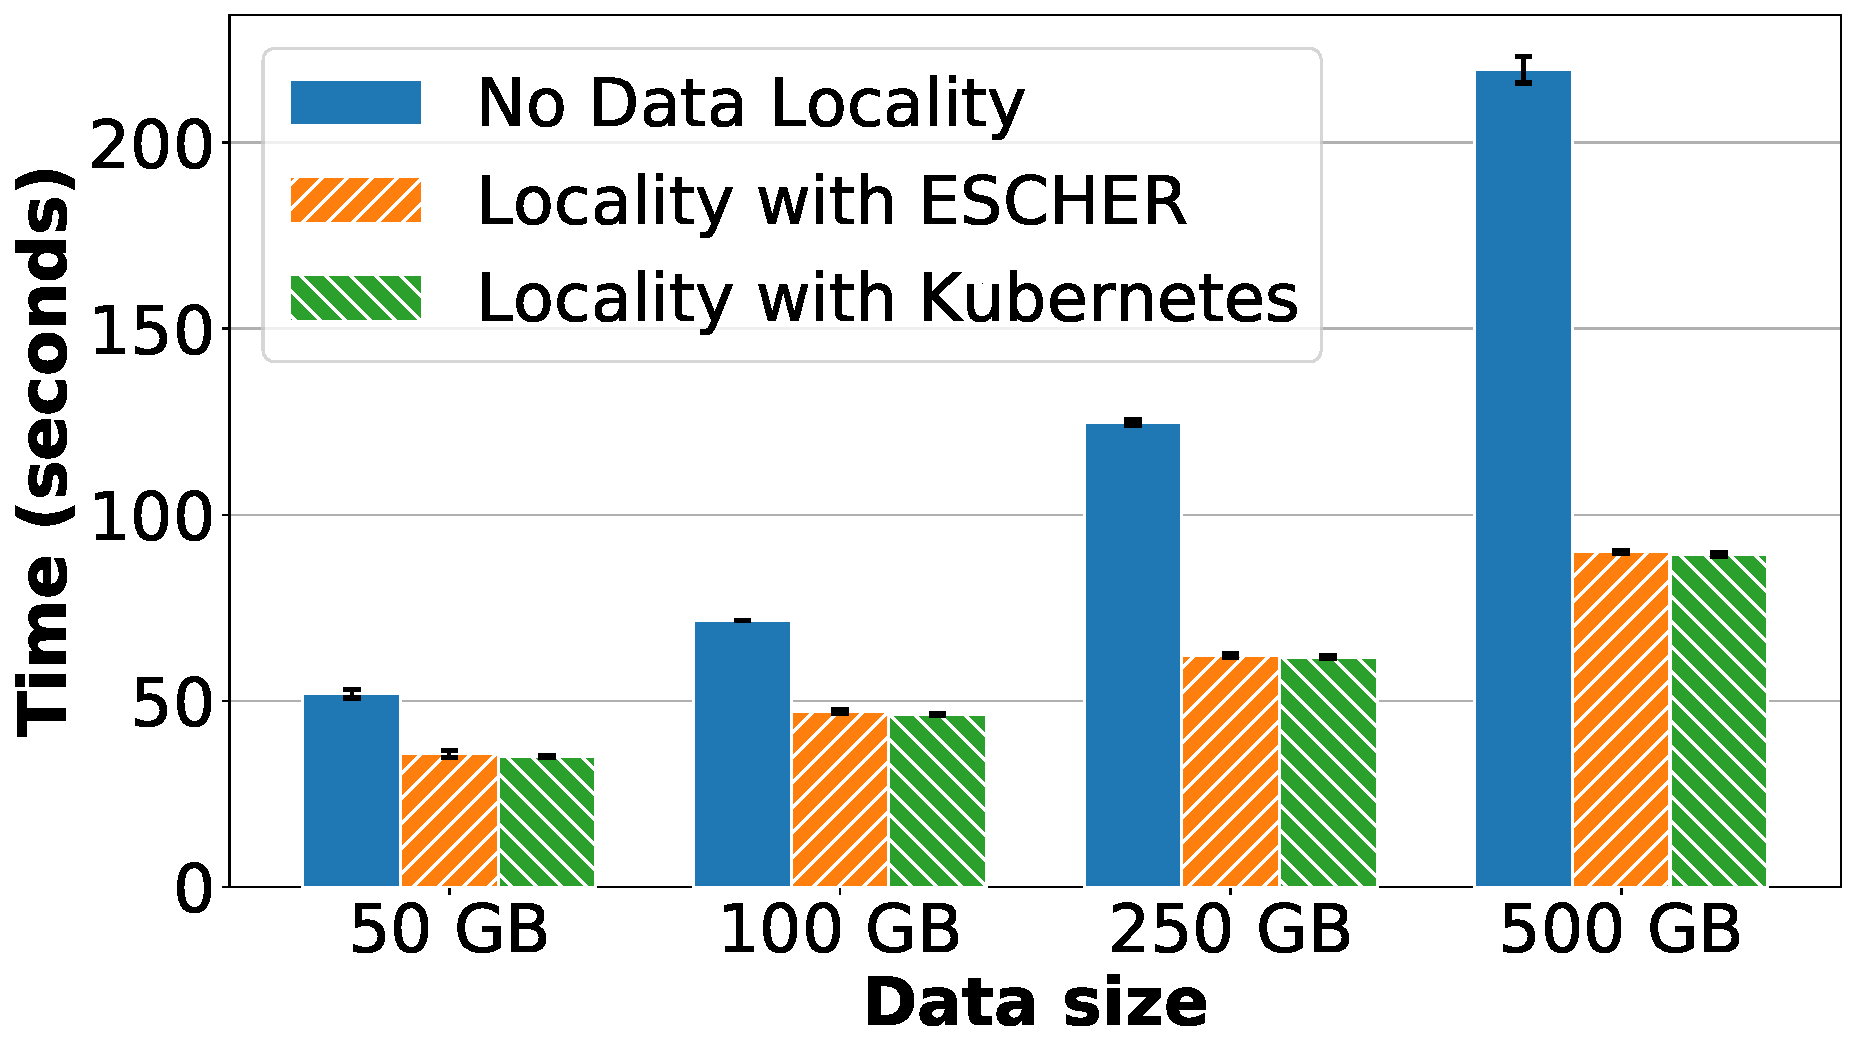
\includegraphics[width=\textwidth]{escher/plots/mapreduce_makespan.pdf}
\caption{
%A random placement policy has high network overheads due to poor data-locality. ESCHER implementation on Kubernetes performs comparably with the off-the-shelf core Kubernetes data locality policy.
}
\label{fig:mapreduce-makespan}
\end{subfigure}
\begin{subfigure}[b]{0.39\textwidth}
\hspace{2mm}
\footnotesize
% \begin{table}[ht]
% \begin{center}
\raisebox{15mm}{
\begin{tabular}{cccc}
% {\tiny
\toprule
& \multicolumn{3}{c}{\textbf{Scheduler}}\\
\textbf{Nodes}     & Generic & Kubernetes & ESCHER \\
\midrule
10 & $183.32 \pm 0.51$ & $54.69 \pm 0.46$ & $55.24 \pm 0.39$ \\\hline
50 & $113.71 \pm 0.49$ & $44.02 \pm 0.27$ & $44.71 \pm 0.44$  \\\hline
100 & $51.90 \pm 0.31$ & $35.08 \pm 0.31$ & $35.76 \pm 0.49$  \\
\bottomrule
% }
\end{tabular}
}
\caption{
% As the cluster size increases, ESCHER scales similarly to core kubernetes scheduler, while outperforming the generic data-locality unaware scheduler.
}
\label{tab:mapreduce-xnode}
%\vspace{-8mm}
% \end{table}
\end{subfigure}
\begin{subfigure}[b]{0.30\textwidth}
 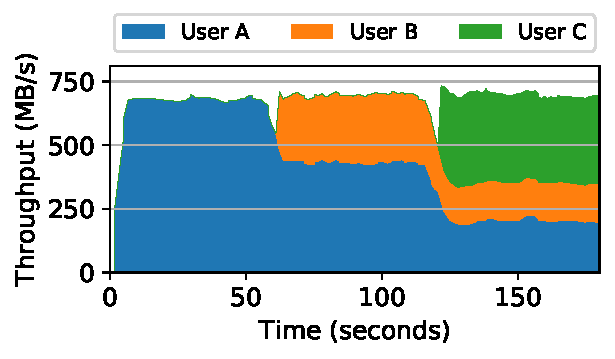
\includegraphics[width=\textwidth]{escher/plots/hfs/3user_hfs_sharing_mapreduce_50nodes_area_short.pdf}
 \caption{}
 \label{fig:hfs-3user-result}
\end{subfigure}
\vspace{-2em}
\caption{\small 
Data locality and hierarchical max-min fair sharing for WordCount.
\textbf{(a)} Makespan of WordCount running on a 100-node Kubernetes cluster, comparing a random placement policy, ESCHER on Kubernetes with data locality, and Kubernetes' native data locality.
\textbf{(b)} Makespan of WordCount MapReduce jobs in seconds across varying cluster sizes.
\textbf{(c)} Hierarchical max-min fair sharing with ESCHER.
A and B are in Sub-Org1 with weights 2:3; C is in Sub-Org2.
A, B, and C begin submitting tasks at $t=$0, 60, and 120, respectively.
}
\vspace{-3mm}
\end{figure*}


\section{Evaluation}
\label{sec:eval}

In this section, we evaluate the following questions:
\begin{compactitem}
    \item Can existing distributed applications be ported to use ESCHER and what are its implications?
    \item What are the tradeoffs with implementing scheduling policies in the application space vs in the framework?
    \item What are the overheads of scheduling with ephemeral resources?
\end{compactitem}

All evaluations use Amazon EC2 m5.12xlarge, m5.4xlarge or p3.8xlarge instances. Kubernetes clusters are provisioned using Amazon EKS running version 1.19.

\subsection{End-to-end Evaluation}
\label{sec:eval:e2e}
% Logical resources act as a thin layer of scheduling indirection for applications without sacrificing framework flexibility.
%In this section, we study four applications and their scheduling requirements. We then demonstrate how \name{} can accelerate these applications by allowing them to express complex scheduling policies with minimal developer effort.

\subsubsection{WordCount with MapReduce}
\label{eval:wordcount}
% What is mapreduce, what is word count
%These chunks are then individually processed by multiple mapper tasks in a distributed fashion. The results of mapper tasks are consumed by reduce tasks which key-wise consolidate the results.
WordCount counts the number of words in large text datasets and is often implemented with MapReduce~\cite{mapreduce}. To avoid expensive data transfers, data locality is essential.
% A data locality policy is essential to performance in this model, since map tasks must be colocated with their assigned inputs (which are usually on disk at a particular node) to avoid expensive data transfers.
% WordCount is a program implemented on the MapReduce~\cite{mapreduce} model to count the number of words in large text datasets. WordCount works by splitting the text file into smaller chunks, distributing them over the network and then running distributed mappers to count word frequency in these chunks.
% How data locality plays in. Implementation, HDFS Spark etc.
% The map tasks in WordCount are highly dependent on their locality with the data chunk they are assigned to process. If the data chunk is not present on the node where the map task is scheduled, it is forced to perform an expensive fetch over the network before starting processing. This dependence makes WordCount a benchmark to stress data-locality.
% Describe setup 100 nodes.
We implement the map and reduce tasks as independent operators running in containers.
The input files are chunks of a file with random words, each hosted by one of 100 nodes. The total input size is varied from 50 GB to 500 GB.
% and use Kubernetes to distribute these tasks over a 100-node cluster.
% The inputs are chunks of a file with random words, each  hosted by one of 100 nodes. 
% The total input size is varied from 50 GB to 500 GB.
%In this setup, the scheduler must place the mapper tasks on the nodes which host their chunk to minimize delays from network transfers.
We implement \name{} on Kubernetes, using an ESL for data locality (\Cref{policies}), and compare against Kubernetes's built-in data-locality policy~\cite{kubernetes-doc} and a locality-unaware random policy.
% For \name{} on Kubernetes, we use an ESL that implements data locality (\Cref{policies}).

% How do it in k8s, ESCHER.
% To achieve this data locality with the default Kubernetes scheduler, we use the \lstinline{NodeAffinityPriority} specifier in the scheduler to place mappers on nodes where their assigned chunk exists. This serves as a baseline to compares against ESCHER. In ESCHER, we create a resource \lstinline{chunk-n} on each node, where $n$ is the id of chunk hosted by the node. The mappers then request this resource to get co-located with their chunk. This policy is wrapped in an ESL which is invoked by WordCount.

Unsurprisingly, \Cref{fig:mapreduce-makespan} shows that as the input size increases, 
%the overhead of data transfer dominates execution if locality is not considered.
the overhead of transferring chunks over the network dominates the mapper computation time for the no-locality policy, taking up to 58.3\% of the total job time when the input size is 500 GB.
Meanwhile, \name{} on Kubernetes provides the same performance as Kubernetes itself, but without modifying the core scheduler framework.
Furthermore, \Cref{tab:mapreduce-xnode} shows that \name{} can also scale with the cluster size. 
%As the cluster size increases, the scheduling sub-system is stressed to distribute more map and reduce tasks.
Throughout different scales, ESCHER performs comparably with the core Kubernetes scheduler, with its makespan staying within $1.9\%$ of the baseline Kubernetes scheduler.. Implementing data locality with ESCHER required adding only two lines:  a \lstinline{set_resource} call during data generation to create a local \lstinline{data-<id>} resource and a line to specify a \lstinline{data-<id>} resource requirement for the mapper tasks.

% Compares against k8s
% Figure \ref{fig:mapreduce-makespan} and \Cref{tab:mapreduce-xnode} compare the makespan across different input and cluster sizes. % for a scheduling policy implemented in ESCHER, the off-the-shelf data-locality scheduler in Kubernetes and a policy which randomly places mappers without any data-locality.
% As the input size increases, the overhead of transferring chunks over the network dominates the mapper computation time for the no-locality policy, taking up to 58.3\% of the total job time when the input size is 500 GB.
% \Cref{fig:mapreduce-makespan} shows that ESCHER on Kubernetes can provide the same application-level benefits as Kubernetes itself, but without modifying the core scheduler framework.
% Furthermore, \Cref{tab:mapreduce-xnode} shows that as the cluster size increases, ESCHER can also scale with the increased number of map and reduce tasks (within $1.9\%$ of the core Kubernetes scheduler).

% As the cluster size increases, the scheduling sub-system is stressed to distribute more map and reduce tasks. Throughout different settings, ESCHER performs comparably with the core Kubernetes scheduler, with its makespan staying within $1.9\%$ of the baseline Kubernetes scheduler. 



% \begin{figure}
% \centering
% 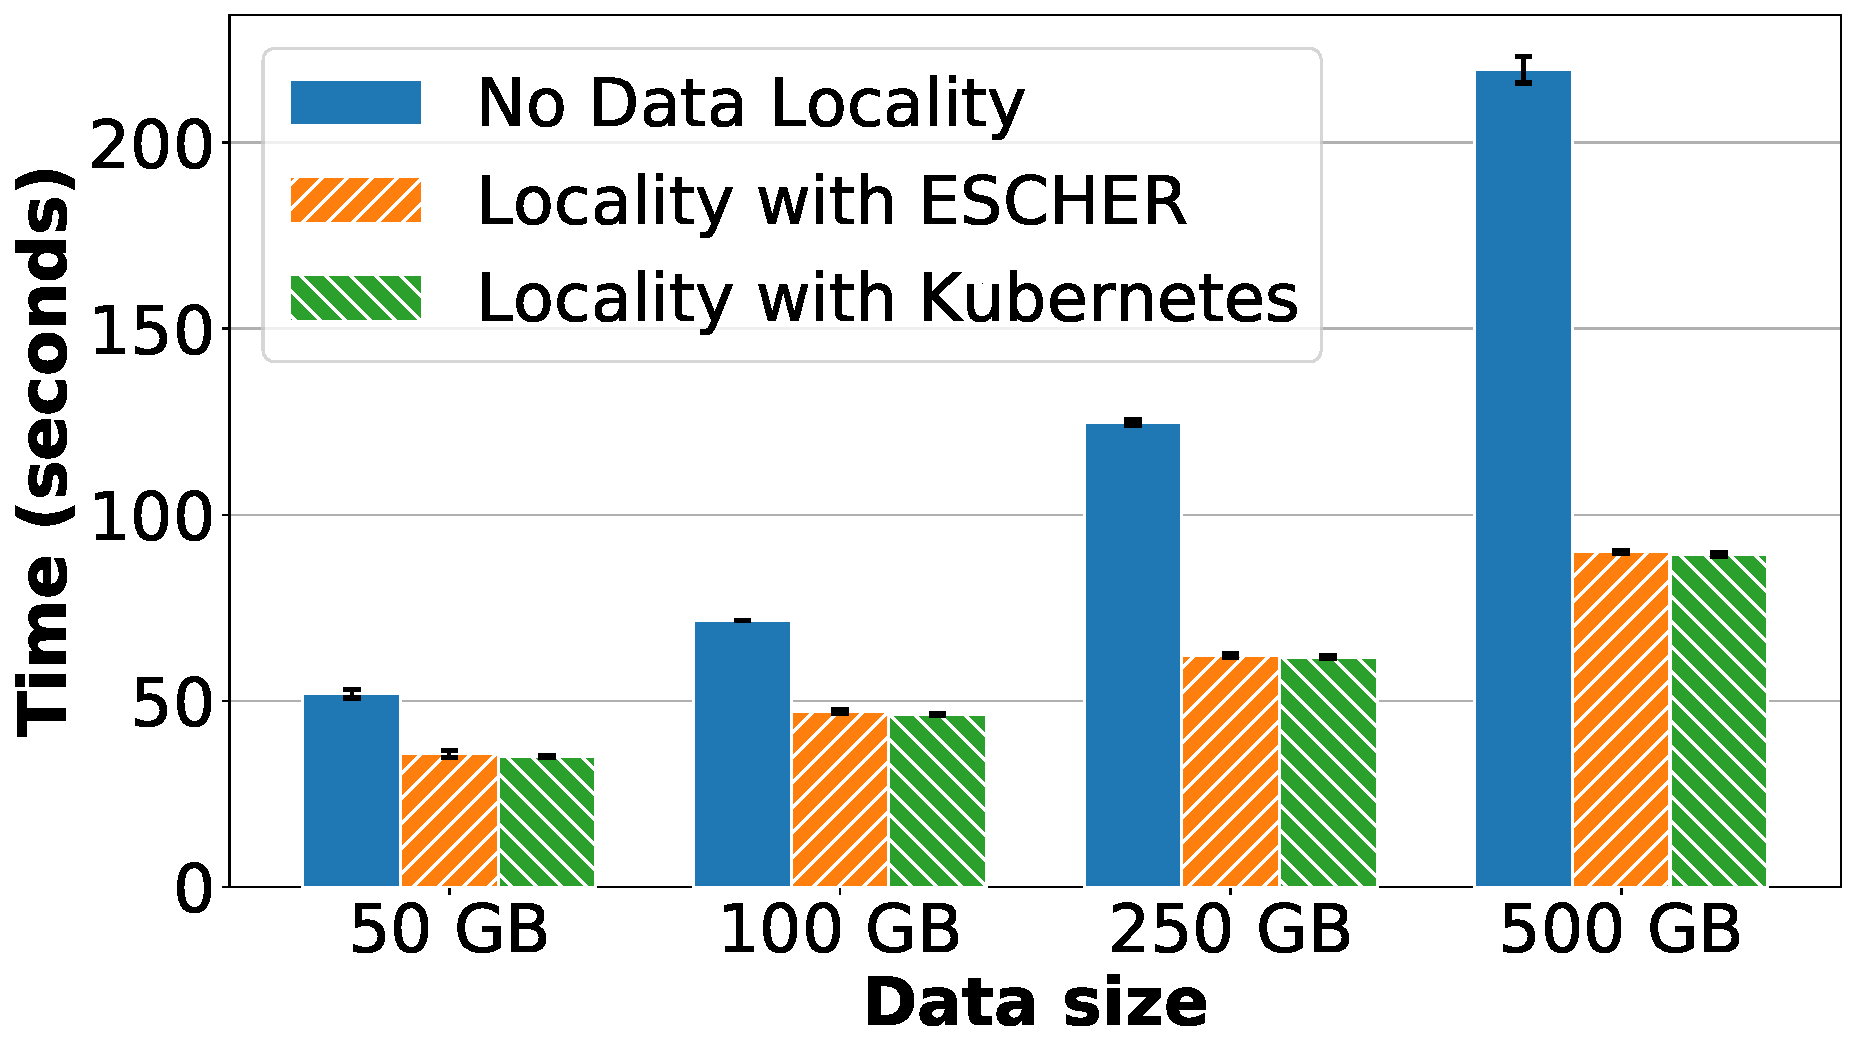
\includegraphics[width=0.8\columnwidth]{escher/plots/mapreduce_makespan.pdf}
% \caption{\small Makespan of WordCount running on a 100-node Kubernetes cluster, comparing a random placement policy, ESCHER on Kubernetes with data locality, and Kubernetes' native data locality.
% %A random placement policy has high network overheads due to poor data-locality. ESCHER implementation on Kubernetes performs comparably with the off-the-shelf core Kubernetes data locality policy.
% }
% \label{fig:mapreduce-makespan}
% \end{figure}

% \begin{table}[ht]
% \begin{center}
% \begin{tabular}{cccc}
% \toprule
% & \multicolumn{3}{c}{\textbf{Scheduler}}\\
% \textbf{Nodes}     & Generic & Kubernetes & ESCHER \\
% \midrule
% 10 & $183.32 \pm 0.51$ & $54.69 \pm 0.46$ & $55.24 \pm 0.39$ \\\hline
% 50 & $113.71 \pm 0.49$ & $44.02 \pm 0.27$ & $44.71 \pm 0.44$  \\\hline
% 100 & $51.90 \pm 0.31$ & $35.08 \pm 0.31$ & $35.76 \pm 0.49$  \\
% \bottomrule
% \end{tabular}
% \end{center}
% \caption{\small Makespan of WordCount MapReduce jobs in seconds, compared across varying cluster sizes.
% % As the cluster size increases, ESCHER scales similarly to core kubernetes scheduler, while outperforming the generic data-locality unaware scheduler.
% }
% \label{tab:mapreduce-xnode}
% %\vspace{-8mm}
% \end{table}


% \begin{figure}[ht]
% % \begin{subfigure}{1\linewidth}
% % \centering
% % 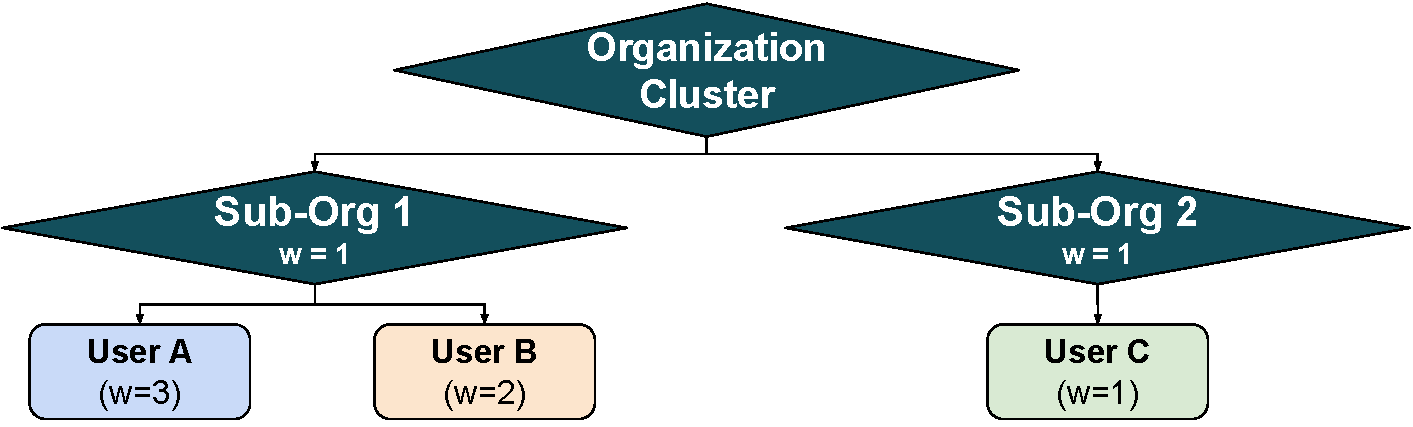
\includegraphics[width=1\columnwidth]{escher/plots/hfs/ESCHER_HFS_3User_OrgChart.pdf}
% % \caption{Organization Chart}
% % \label{fig:hfs-3user-orgchart}
% % \end{subfigure}
% % \begin{subfigure}{1\linewidth}
% \centering
% 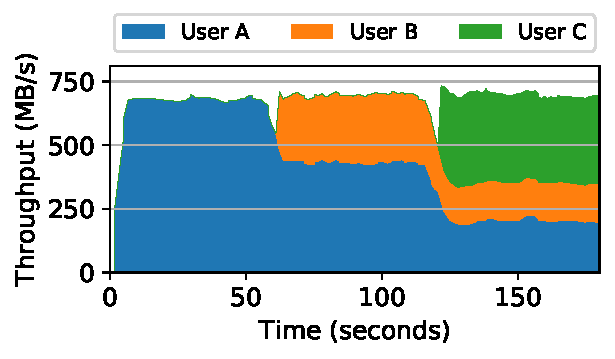
\includegraphics[width=0.93\columnwidth]{escher/plots/hfs/3user_hfs_sharing_mapreduce_50nodes_area_short.pdf}
% % \caption{User-wise throughput}
% % \end{subfigure}
% \caption{\small Per-user WordCount throughput with hierarchical max-min fair sharing.
% A and B are in Sub-Org1 with weights 2:3; C is in Sub-Org2.
% A, B, and C begin submitting tasks at $t=0,60,120$, respectively.
% %(a) shows the organization chart for resource sharing between sub-org 1 and sub-org 2. Weights (w) are relative to other users under the same parent.
% % (b) plots the throughput for users A, B and C on a cluster of 50 nodes.
% %At time t=0, only user A is submitting tasks so the HFS ESL allocates all resources to user A. At time t=60 and t=120, User B and User C start submitting tasks respectively.
% % The HFS ESLs adjust resource allocations based on utilization while maintaining organization level and sub-organization level weight proportional fairness.
% }
% \label{fig:hfs-3user-result}
% \end{figure}
% Two interfaces - infeasible and cancel tasks
% Throughput bug

% \begin{figure}
% \begin{subfigure}{1\linewidth}
% \centering
% 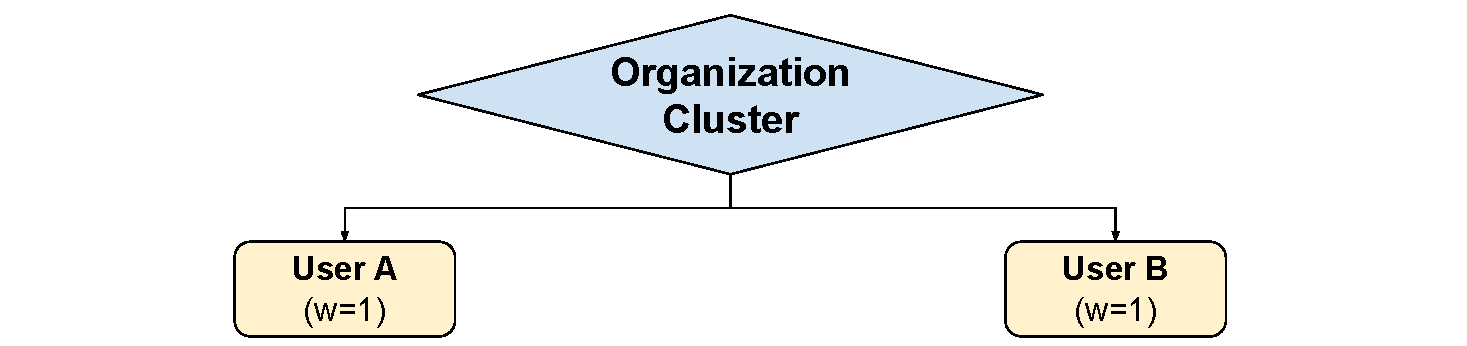
\includegraphics[width=1\columnwidth]{escher/plots/hfs/ESCHER_HFS_2User_OrgChart.pdf}
% \caption{Organization Chart}
% \label{fig:hfs-2user-orgchart}
% \end{subfigure}
% \begin{subfigure}{1\linewidth}
% \centering
% 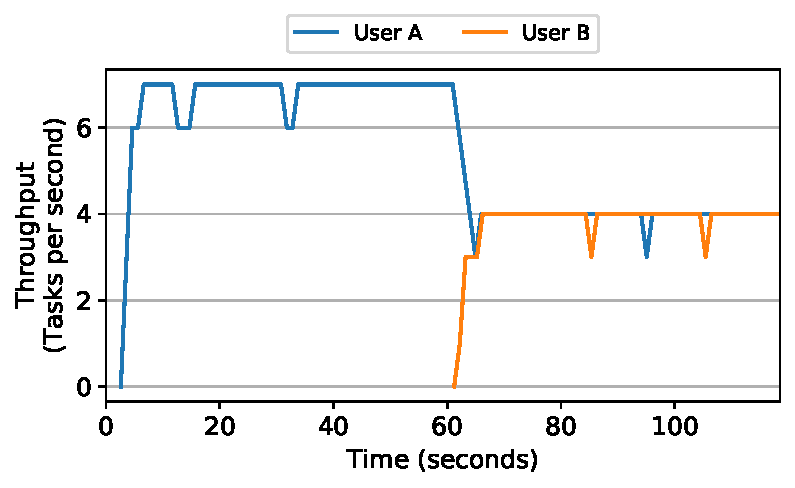
\includegraphics[width=0.9\columnwidth]{escher/plots/hfs/2user_hfs_sharing.pdf}
% \caption{User-wise throughput}
% \label{fig:hfs-2user-result}
% \end{subfigure}
% \caption{\small Min-Max Fair Sharing with ESCHER. Figure (a) shows the organization chart for resource sharing between User A and User B, each having equal weights (w=1). Figure (b) plots the throughput for users A and B. At time t=0, only user A is submitting tasks so the HFS ESL allocates all resources to user A. At time t=60 user B starts submitting tasks. The HFS ESL adjusts deallocates resources from user A and reassigns them to user B to maintain fairness.  
% }
% \label{fig:hfs-2user}
% \end{figure}

\subsubsection{Hierarchical max-min fair sharing}
\label{eval:hfs}
% Cool bits:
% \begin{itemize}
%     \item The resizing of the cluster is completely transparent to the users - they don't need to worry how many resources are allocated to them
%     \item Composition of data locality and fair sharing is as simple as adding resource requirements.
% \end{itemize}
Hierarchical Max-Min Fair Sharing (\Cref{policies}) allocates resources proportionate to a user's weight in a hierarchical organization.
% HFS maximizes resource utilization by reallocating idle resources.
Users submit jobs at different times, so their ideal absolute resource share is dynamic, making it impossible to maximize overall resource utilization with static labels.
% This makes it impossible to implement HFS with a static label-based scheduler since the resource share per user is dynamic.
For example, consider a two-team organization: Sub-Org1 with users A and B of weights 2:3, and Sub-Org2 with user C.
% with equal weights - Sub-Org1 and Sub-Org2. Sub-Org1 has two users, A and B with weights 2:3, while sub-org2 has one user C.
To ensure fairness with static labels, the only option is to allocate each user a fixed proportionate share, leading to under-utilization when only one user is submitting work.

% To achieve fairness, the only option with static labels would be to allocate each user a fixed share, leading to under-utilization in \Cref{fig:hfs-3user-result}. (i.e., A would only reach 200MB/s at $t$=0).

Because ephemeral resources can be \emph{dynamically} created and destroyed, an HFS policy ensures fairness while also maximizing overall utilization as users enter and leave the system~(\Cref{fig:hfs-3user-result}).
We deploy a HFS policy on a 100 node cluster running WordCount. We use a parent ESL for the teams and two children ESLs for Sub-Orgs 1 and 2 to create a hierarchy of ESLs.
An HFS ESL tracks idle resources and reallocates resources between teams or users.
% For example, at $t$=60 in \Cref{fig:hfs-3user-result}, B begins submitting tasks, causing the Sub-Org1 ESL to reclaim resources from A.
The workload in \Cref{fig:hfs-3user-result} starts with only user A submitting tasks to the scheduler. Since other users' resources are idle, the HFS ESLs re-allocate all idle resources to A to achieve max-min fairness. At time $t$=60, user B starts submitting tasks. This causes the Sub-Org 1 ESL to reclaim resources from A to re-allocate to B, in proportion to their weights. B's warmup time causes a small dip in net throughput at $t$=60. Finally at time $t$=120, user C starts submitting tasks and the parent ESL reallocates resources to Sub-Org2. Since Sub-Org 2 and Sub-Org 1 have equal weights, C's resource allocation is equal to the sum of A and B's allocation.
Ephemeral resources also enable composition: the application composes its custom policy (in this case, data locality for WordCount) with the two HFS ESLs by concatenating all the resource requirements.

% The workload in \Cref{fig:hfs-3user-result} starts with only user A submitting tasks to the scheduler. Since other users' resources are idle, the HFS ESLs re-allocate all idle resources to A to achieve max-min fairness. At time $t$=60, user B starts submitting tasks.
% This causes the Sub-Org 1 ESL to reclaim resources from A to re-allocate to B, in proportion to their weights. B's warmup time causes a small dip in net throughput at $t$=60. Finally at time $t$=120, user C starts submitting tasks and the parent ESL reallocates resources to Sub-Org2. Since Sub-Org 2 and Sub-Org 1 have equal weights, C's resource allocation is equal to the sum of A and B's allocation.

% Not only is ESCHER able to maintain the cluster's fair-sharing requirements, it also allows the each user to compose their application-level policies with cluster-level policies. This is achieved by simply concatenating the data-locality resources with the resource requirement vector from the fair-sharing ESL. This concatenation ensures that the scheduler places the tasks where both constraints - fairness and data-locality - can be satisfied.

% Using ephemeral resources also reduces implementation complexity by enabling transparent resizing of user shares when applying max-min fairness. Since the ESLs dynamically create and removes each user's ephemeral resources from underlying nodes, the users' applications are not required to keep a track of the resources allocated to them. This would not have been possible in a static label-based scheduler since the max-min shares for each user are dynamic. 



\subsubsection{AlphaZero}
AlphaZero \cite{silver2017mastering} is a reinforcement learning application for the board game Go.
%Unlike it's predecessor AlphaGo\cite{silver2016alphago}, AlphaZero does not require any human-generated training samples and can instead leverage reinforcement learning techniques to play and learn from games against itself.
%We base this experiment off an existing AlphaZero implementation \cite{anthony2017thinking}, which uses hard-coded process placement.
We demonstrate \name{}'s flexibility by porting an implementation~\cite{anthony2017thinking} onto Ray without compromising performance relative to the optimal hard-coded (but inflexible) placement.

AlphaZero executes a Monte Carlo Tree Search on the game state space in a CPU-intensive \textit{BoardAggregator} process. The search is guided by a \textit{PredictorAgent} running a neural network on a GPU which evaluates a board and predicts the associated reward.
%Based on this prediction, the \textit{BoardAggregator} generates new boards to explore and learn from.
% This pattern creates a tight feedback loop between the \textit{BoardAggregator} and the \textit{PredictorAgent}.
Co-locating \textit{BoardAggregator}s and their corresponding \textit{PredictorAgent}s on the same physical node is thus desirable to avoid network overheads from transferring board states. These pairings also require anti-affinity for load balancing and to avoid interference \cite{gandiva}.
%Many existing frameworks do not allow the expression of this composition of load-balancing and co-location policies, while others frameworks would require a tedious re-implementation of the scheduler. 
With ephemeral resources, this composed policy can be specified in 5 lines of code~(\cref{fig:alphazerocode}): we apply a load-balancing policy~(\Cref{tab:escher-constraints-policies}) to the \textit{PredictorAgent} and a co-location policy to the \textit{BoardAggregator} and \textit{PredictorAgent}.
%This composition takes only 5 lines of code (\cref{fig:alphazerocode}).

We ran 10k iterations of AlphaZero on a 32-node cluster (128 GPUs total). %board generation distributed across 16 machines with a total of 128 GPUs.
We compare three setups: 
(a) co-location with hard-coded placement,
(b) co-location with ephemeral resources, and 
(c) a baseline policy with no co-location. 
\Cref{fig:alphazerolatencycdf} plots the CDF for board exploration time. %, which includes generating the board on the \textit{BoardAggregator} and evaluating it on the \textit{PredictorAgent}. 
% Comparing the percentile distributions from this CDF in \cref{fig:alphazerolatencypxx}
Co-location is important for performance, outperforming no-colocation by 15.4\% in median latency and 20\% in P95 latency. %, demonstrating the benefits of co-location.
Additionally, co-location with ephemeral resources adds insignificant overheads of <1\%, while requiring less developer effort: the application code~(\Cref{fig:alphazerocode}) does not need to match \textit{PredictorAgent}-\textit{BoardAggregator} pairs to specific nodes.

% while providing a much simpler interface to express scheduling requirements.

%and by 714\% on P99.9 latency. P99.9 latency demonstrates the largest difference because the initial queries in the no-colocation case require setting up inter-machine communication sockets which may take time.

% Co-location with Logical Resources Stats - P999: 0.05949, P95: 0.02135, P50: 0.02083
% Static Co-location Stats - P999: 0.05863, P95: 0.02147, P50: 0.02079
% No Co-location Stats - P999: 0.06227, P95: 0.02578, P50: 0.02401


% \begin{figure}
% ~
% % Task co-location
% ~
% \begin{subfigure}{.22\textwidth}
%   \centering
%   \begin{minted}[fontsize=\tiny,breaksymbolleft=\tiny\ensuremath{},breakautoindent=true]{python}
% class PredictorAgent():
%   def __init__(id):
%     # Create resource for co-location
%     set_resource(label=id, capacity=1)
%     ...
%   \end{minted}
% \end{subfigure}
% ~
% % Task co-location
% ~
% \begin{subfigure}{.22\textwidth}
%   \centering
%   \begin{minted}[fontsize=\tiny,breaksymbolleft=\tiny\ensuremath{},breakautoindent=true]{python}
% class BoardAggregator():
%   def __init__(predictor):
%     # Assign predictor handle
%     self.predictor = predictor
%     ...
%   \end{minted}
% \end{subfigure}

% \newline

% \begin{subfigure}{.49\textwidth}
%   \centering
%   \begin{minted}[fontsize=\tiny,breaksymbolleft=\tiny\ensuremath{},breakautoindent=true]{python}
% def main():
%     # Create load-balancing resources
%     for node in cluster:
%         set_resource("load_bal", 1, node)
%     for i in range(0, num_agents):
%         p = PredictorAgent(resources = {"GPU": 1, "load_bal": 1}).launch(id=i)
%         # The predictor creates a resource with label i
%         # This resource is used by the BoardAggregator to co-locate.
%         b = BoardAggregator(resources = {i: 1}).launch(predictor=p)
%   \end{minted}
% \end{subfigure}
% \caption{AlphaZero placement preferences with \name{}}
% \label{figure:alphago}
% \end{figure}

\subsubsection{Distributed Training}
\label{sec:eval:tune}


% \begin{figure}
% 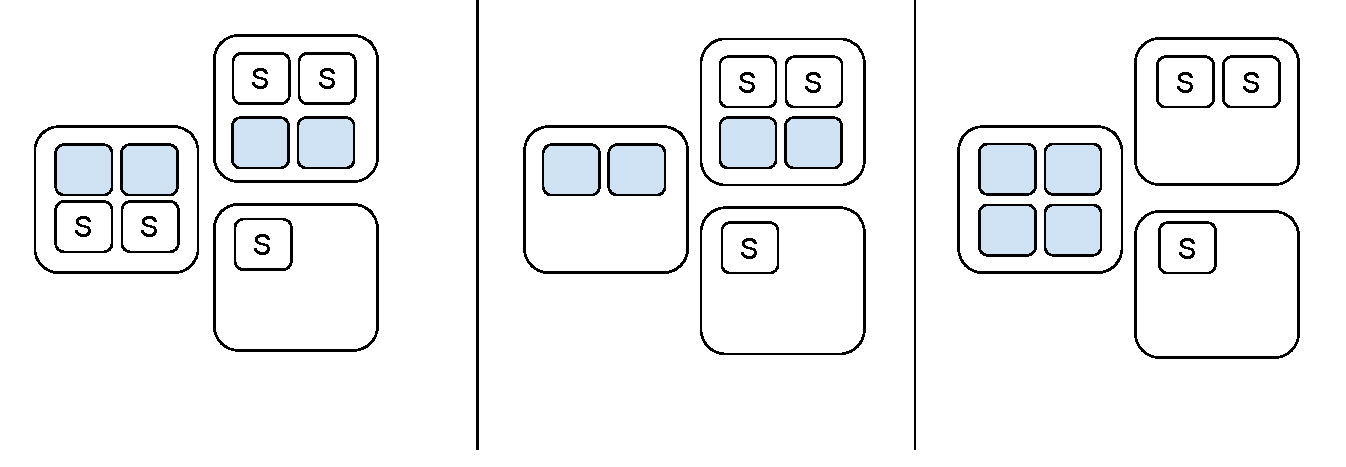
\includegraphics[width=0.9\columnwidth]{escher/figures/Eschertune.pdf}
% \caption{Migration after termination of the Short Job, signaling EscherTune to utilize a co-location mechanism and decrease communication overhead compared to Tune.
% }
% \label{fig:tune-results}
% \end{figure}



\def\longjob{\emph{long-job}}
\def\shortjobs{\emph{short-jobs}}
% Distributed training for a ML model typically consists of multiple workers that compute model updates in parallel and in lockstep.
For a distributed training job, worker placement is critical to performance, as co-locating workers reduces the cost of model synchronization at each step.
% The placement of these workers in a cluster is critical to the performance of the training process, as co-located workers avoid the network cost of model synchronization on each update operation.
%Typically, multiple jobs, each with different size and unpredictable completion time, will execute in parallel as part of a hyperparameter search~\cite{liaw2018tune}.
% Moreover, training jobs in a shared cluster can be of different sizes and with unpredictable completion times.
Gandiva \cite{gandiva} is a scheduler for deep learning jobs that aims to optimize training job performance. It composes a higher level \textit{load-balancing} policy and a lower-level \textit{co-location} policy to evenly spread jobs across machines while reducing intra-job communication overhead. 
To demonstrate \name{}'s flexibility, we augment Gandiva's \cite{gandiva} worker co-location and migration policy with Gang Scheduling to support distributed training jobs, and integrate the policy into Tune \cite{liaw2018tune}, an open source distributed training library built on Ray \cite{ray-osdi}, which we will refer to as \textit{EscherTune}.
We modified the Trial abstraction in Tune to be wrapped in a ghost task that ensures gang scheduling and applied co-location on tasks belonging to the same Trial.
%EscherTune records the current cluster placements during execution.
EscherTune triggers a migration whenever it detects sufficient available resources to place all workers of a job on the same node.
To execute a worker migration, EscherTune checkpoints the current job using application-specific checkpoint functionality and destroys all current workers. Then, EscherTune assigns ephemeral resources to the new target node, and relaunches all worker tasks of the training job without modifying their ephemeral resource requests.
 %To execute a worker migration, EscherTune will checkpoint the current training job using framework-dependent checkpoint functionality and destroy all current workers. Then, EscherTune assigns ephemeral resources to the target node and relaunches all worker processes of the training job with the specified ephemeral resource requests.
 
We compare EscherTune with Tune's open-source policy on a cluster of 12 GPUs. We launch 5 short-running training jobs (\shortjobs{}), each requiring 1 GPU, followed by 1 long-running training job requiring 4 GPUs (\longjob{}).
Each training job is training a ResNet-101 model on CIFAR-10 with a batch-size of 64 images per device.

Initially, the \shortjobs{} are load-balanced across the cluster, while the 4 workers of the \longjob{} are spread across the cluster depending on GPU availability. This is a sub-optimal placement, so EscherTune migrates the \longjob{} to colocate its tasks as soon as resources become available from a \emph{short-job} completion, resulting in 36.3\% higher throughput~(\Cref{fig:tune-results}).
Meanwhile, Tune uses a static placement, so the \longjob{}'s throughput remains the same.
% Figure \ref{fig:tune-results} compares throughput of \longjob{} in EscherTune and Tune, with all jobs launched at the same time. The throughput is low when the workers are spread across the cluster, but when there are sufficient resources to place workers on the same node, EscherTune is able to use ephemeral resources to migrate and co-locate all workers, increasing the throughput of the job by 36.3\%.
Furthermore, EscherTune's implementation consists of only 50 lines of Python, with no changes to Tune or the Ray scheduler. % a callback of 50 lines of Python, with \textit{no changes} to Tune.
 

% \begin{figure}[t]
% \centering
% 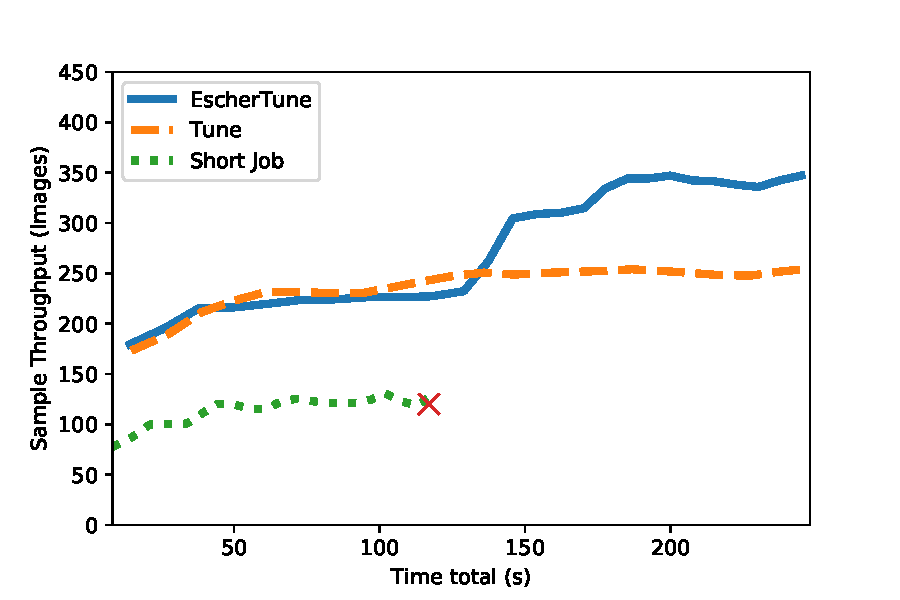
\includegraphics[width=0.85\columnwidth]{escher/plots/result_migrationthroughput.pdf}
% \caption{\small Throughput comparison of distributed training workloads with and without migration. ESCHER is able to augment an existing application, Tune, to increase sample throughput. 
% The red X indicates the termination of the short job, signaling EscherTune to utilize the co-location mechanism and decrease communication overhead compared to Tune.
% }
% % \caption{Throughput comparison of distributed training jobs with and without migration. 
% % Sample throughput for training can increase significantly by co-locating workers of
% % a distributed training job. In this mixed workload containing a distributed training job for a ResNet-101 architecture using 4 workers, ESCHER is able to easily augment the underlying framework to significantly improve performance. 
% % The red X indicates the termination of the Short Job, signaling EscherTune to utilize a co-location mechanism and decrease communication overhead compared to Tune.
% % }
% \label{fig:tune-results}
% \vspace{-0.3in}
% \end{figure}

% \subsubsection{Implementing Kube-Batch with ESCHER}
% To demonstrate ESCHER's ease-of-use, we add Gang Scheduling to Kubernetes using the Ephemeral Resources API and compare the implementation with a plug-in scheduler which adds this functionality to kubernetes. As described in Section \ref{sec:motivation}, adding gang scheduling to Kuberenetes in it's current form has been possible only through separate plug-in schedulers. One such plug-in is kube batch
\begin{figure*}[t]
\begin{subfigure}[b]{0.47\linewidth}
  \centering
\begin{subfigure}[t]{.22\textwidth}
  \centering
  \begin{minted}[fontsize=\tiny,breaksymbolleft=\tiny\ensuremath{},breakautoindent=true]{python}
class PredictorAgent():
  def __init__(id):
    # Create co-location resource.
    set_resource(
      name=id,
      capacity=1)
    ...
  \end{minted}
\end{subfigure}
~
% Task co-location
~
% \begin{subfigure}[b]{.21\textwidth}
%   \centering
%   \begin{minted}[fontsize=\tiny,breaksymbolleft=\tiny\ensuremath{},breakautoindent=true]{python}
% class BoardAggregator():
%   def __init__(predictor):
%     # Assign predictor handle
%     self.predictor = predictor
%     ...
%   \end{minted}
% \end{subfigure}
\begin{subfigure}[t]{0.72\textwidth}
  \centering
  \begin{minted}[fontsize=\tiny,breaksymbolleft=\tiny\ensuremath{},breakautoindent=true]{python}
def main():
  # Create load-balancing resources
  for node in cluster: set_resource("load_bal", 1, node)
  for i in range(0, num_agents):
    p = PredictorAgent(resources = {"GPU": 1, "load_bal": 1}).launch(id=i)
    # The predictor creates a resource with label i
    # This resource is used by the BoardAgg to co-locate.
    b = BoardAggregator(resources = {i: 1}).launch(p)
  \end{minted}
\end{subfigure}
  \caption{}
  \label{fig:alphazerocode}
\end{subfigure}
\begin{subfigure}[b]{0.26\textwidth}
  \centering
  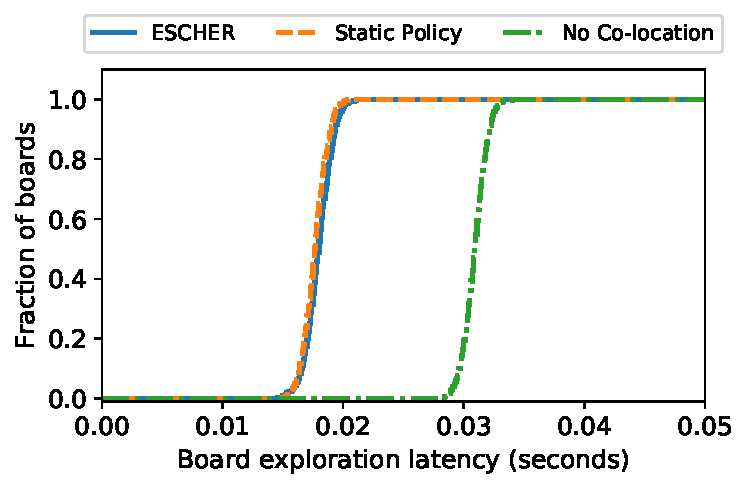
\includegraphics[width=\textwidth]{escher/plots/results_e2e_alphago_latencycdf_16node.pdf}
  \caption{}
  \label{fig:alphazerolatencycdf}
\end{subfigure}
\begin{subfigure}[b]{0.26\textwidth}
\centering
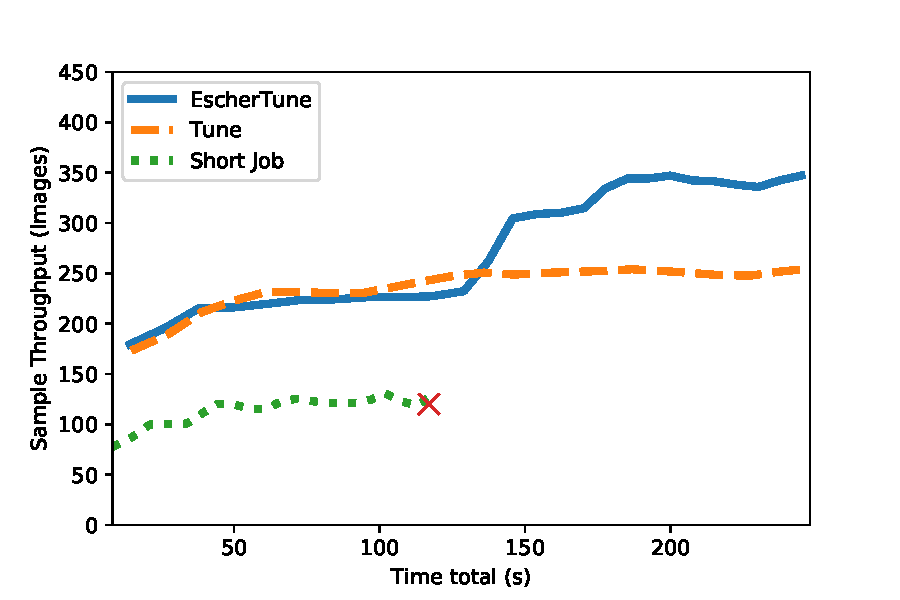
\includegraphics[width=\textwidth,trim=0cm 0cm 1.5cm 0cm, clip]{escher/plots/result_migrationthroughput.pdf}
\caption{}
\label{fig:tune-results}
\end{subfigure}
% \begin{subfigure}[b]{0.3\textwidth}
%   \centering
%   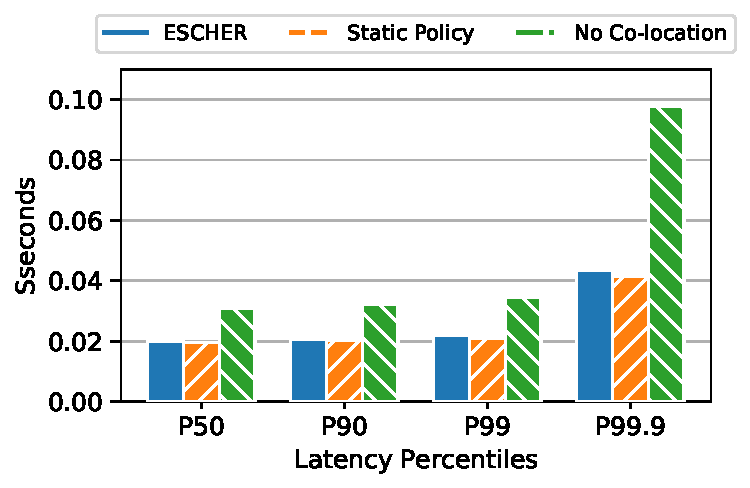
\includegraphics[width=\textwidth]{escher/plots/results_e2e_alphago_pxxcompare_16node.pdf}
%   \caption{}
%   \label{fig:alphazerolatencypxx}
% \end{subfigure}
\caption{\small AlphaZero and distributed training on \name{}. \textbf{(a)} Implementing AlphaZero policy with ESCHER, composing co-location with load-balancing.
% By co-locating the \textit{BoardAggregator}s and the \textit{PredictorAgent}s, the \name{} takes significantly lower time to generate and evaluate board states than an unaware scheduler. \name{} also performs comparably with a static policy that hard codes placement decisions, while offering the flexibility of a general scheduling policy.
\textbf{(b)} A CDF of AlphaZero board exploration latency, and
\textbf{(c)} Throughput comparison of a distributed training workload with a mix of short-running and long-running jobs. EscherTune is an augmentation of the hyperparameter search framework Tune~\cite{liaw2018tune}, using ESCHER to dynamically re-schedule jobs as others complete. %SCHER augments an existing application, Tune, to increase sample throughput. 
The red X indicates the completion of a short job. %, and EscherTune re-schedules the long-running job to claim the idle resources. % to utilize the co-location mechanism and decrease communication overhead compared to Tune.
}
\label{fig:alphazerolatencyfigure}
\vspace{-2mm}
\end{figure*}


\begin{figure}[t]
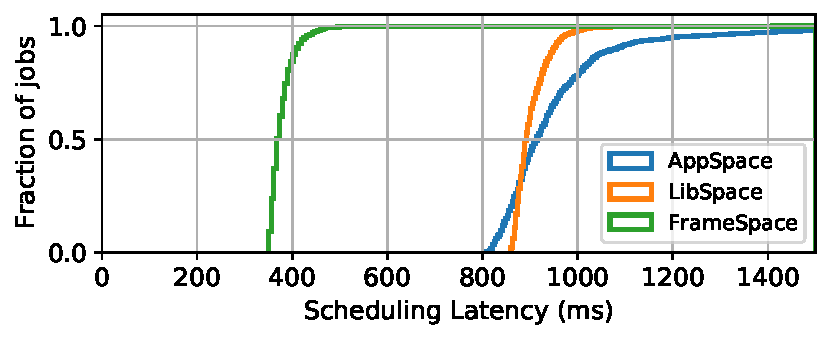
\includegraphics[width=0.92\columnwidth]{escher/plots/result_gangsched_design_compare.pdf}
\caption{\small Request latency for gang scheduling implemented in the application space, with (\textit{LibSpace}) and without (\textit{AppSpace}) coordination, versus the framework space (\textit{FrameSpace}). \textit{FrameSpace} is 1624 lines of code (LoC), \textit{LibSpace} with 261 LoC and \textit{AppSpace} with 78 LoC.}
\label{fig:gangscheddesign-results}
\end{figure}

\subsection{Microbenchmarks}
\subsubsection{Overhead of application-level policies}
\label{sec:eval:gangscheduling}
ESCHER scheduling policies can be implemented either in the application space for evolvability or in the framework for performance.
We evaluate the trade-offs involved in this choice by comparing three distinct designs of gang scheduling, all with ephemeral resources on Ray.

\textit{AppSpace} uses ghost tasks to atomically reserve resources (\Cref{policies:gangsched}).
% An application can call this policy without any coordination with another application in the same cluster.
While this policy is simple to integrate, the lack of coordination between applications can lead to deadlock, which must be resolved through timeouts. %it uses expensive ghost tasks to reserve resources and must resolve any livelocks through expensive timeouts.
\textit{LibSpace} avoids this by using a \emph{shared library}: a shared service in the cluster that serializes gang scheduling requests across applications.
% An application using \textit{LibSpace} sends all gang scheduling requests to this service, which returns the set of ephemeral resources that should be specified when submitting tasks.
\textit{LibSpace} thus avoids live lock entirely but requires deploying a separate shared service.
% \textit{LibSpace} improves upon this by using the same ghost task approach, but in a shared library which runs as a common service in the cluster to provide inter-job coordination. All jobs must communicate with this library to request gang scheduling of their tasks by specifying the resources required for scheduling all tasks. The library returns a ephemeral resource that must then be used by the application to place its tasks. \textit{LibSpace} is able to serialize gang scheduling across jobs, allowing it to avoid live-locks.
Finally, \textit{FrameSpace} modifies the Ray scheduler to expose a gang scheduling API.
Internally, a centralized service within Ray directly reserves and creates ephemeral resources.
Since it has direct access to the resource table, \textit{FrameSpace} avoids using ghost tasks, reducing overheads from worker allocation and task dispatch.

% implements gang scheduling as a part of the core Ray scheduler. This requires modifications in the core ray scheduler to expose an API for applications to request gang scheduling of their tasks. Internally, this implementation directly reserves resources in the scheduler's resource availability map and creates an ephemeral resource which is returned and requested by tasks to schedule their gang of tasks. 

\Cref{fig:gangscheddesign-results} compares the request latency of these designs on a 32-node cluster with 256 CPUs.
% We subsample 100k gang-scheduling requests from the Google ClusterData 2011 trace~\cite{clusterdata:Reiss2011}. % and measure the scheduling latency per request. %and measure the time taken from request submission to job start (scheduling latency).
% We subsample the Google ClusterData 2011 trace \cite{clusterdata:Reiss2011} to model request arrival patterns. 
% To evaluate the performance of these designs, we set up a cluster of 32 nodes with 8 CPUs each. We then submit 100k gang-scheduling requests over 15 minutes and measure the scheduling latency per request. %and measure the time taken from request submission to job start (scheduling latency).
% We subsample the Google ClusterData 2011 trace \cite{clusterdata:Reiss2011} to model request arrival patterns. Figure \ref{fig:gangscheddesign-results} compares the scheduling latency across the three designs.
While the mean latency of \textit{AppSpace} and \textit{LibSpace} is similar, \textit{AppSpace} has higher variance and a longer tail because it uses timeouts to break deadlocks.
\textit{LibSpace} incurs overhead from serializing requests at a separate service, resulting in a higher minimum latency. On average, \textit{FrameSpace} is nearly $2\times$ faster than \textit{AppSpace} and \textit{LibSpace} because it directly reserves resources instead of using ghost tasks. However, we note that for long-running tasks such as model training and batch processing workloads, the absolute scheduling latency is still a tiny fraction (<1s) compared to the runtime of the workloads (multiple hours). Moreover, implementing \textit{FrameSpace} is a significant effort, requiring a deep understanding of the Ray scheduler and modifying 1624 lines of Ray code.
To compare, \textit{LibSpace} and \textit{AppSpace} are implemented in 261 and 78 lines of \emph{application-level} code, respectively.



\subsubsection{Overheads of Ephemeral Resources}
% In this section, we evaluate the costs of introducing ephemeral resources in the framework scheduler.


%\textbf{Dynamic resource creation.}
%Scheduling with ephemeral resources relies on the ability to create and modify resources at run-time.
We evaluate the time to create resources and propagate their availability throughout the cluster.
Since the \lstinline{set_resource} call is asynchronous, we verify that the resources have been created and are available for use by launching no-op tasks that request these newly created resources. %The completion of these tasks marks the successful creation and propagation of ephemeral resources.
% \begin{figure}
%     \centering
%     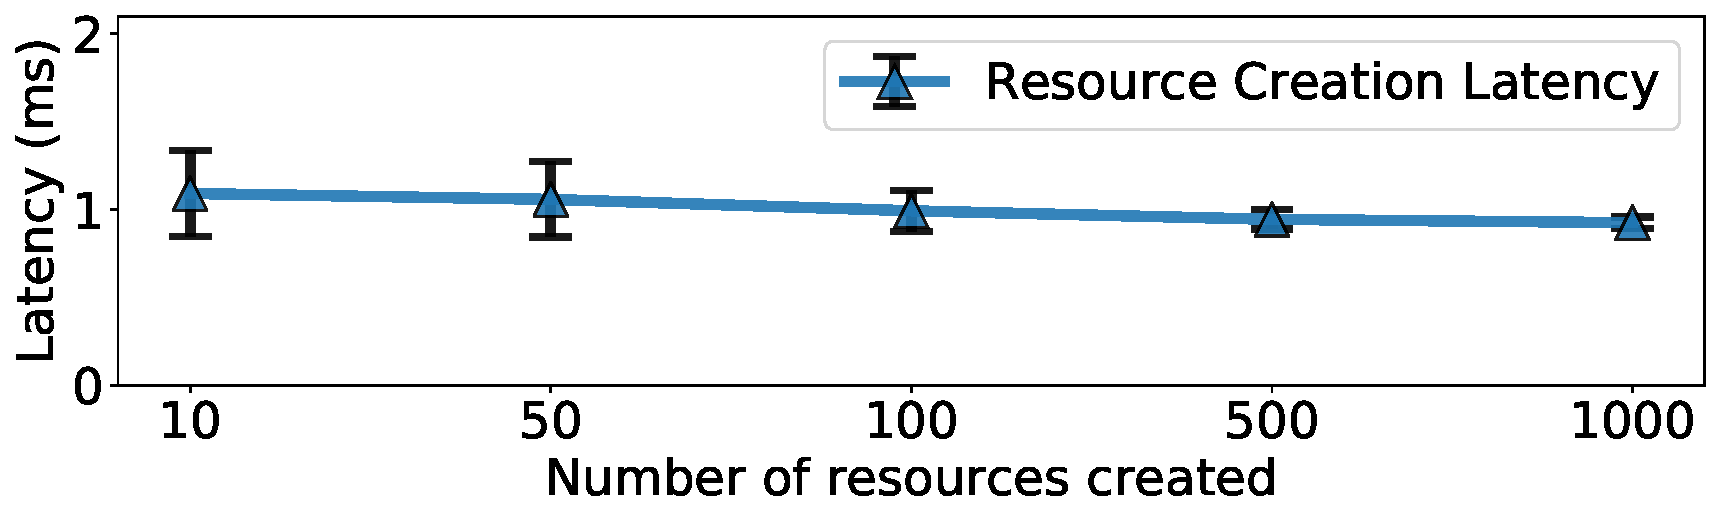
\includegraphics[width=\linewidth]{escher/plots/result_microbench_creationlatency_vs_numres.pdf}
%     \caption{\small Mean per-resource creation latency in Ray. Creating ephemeral resources in \name{} is a low cost operation that scales linearly with the number of resources created.}
%     \label{fig:res-creation-microbench}
% \end{figure}
Figure \ref{fig:res-creation-microbench} compares the mean latency of creating an equal number of resources on each node in a 50-node \ray{} cluster.
We show that even when creating 1000 ephemeral resources, we can maintain 1ms latency per request.
% against the number of resources created using the \lstinline{set_resource} API.
%Number of resources reflects the total resources created in the cluster, while the mean time to resource creation is measured as the time taken from the \lstinline{set_resource} submission to the availability of the resource.
As more resources are created, the cost of resource creation is amortized and the per-resource creation cost decreases to 0.72ms. 
In general, the overhead of creating or deleting an ephemeral resource should be roughly equivalent to that of a key-value store request.
% In absolute terms, the cost of creating ephemeral resources is insignificant, making \name{} a viable design.



\begin{figure*}[t]
\centering
\begin{subfigure}[b]{0.31\linewidth}
  \centering
  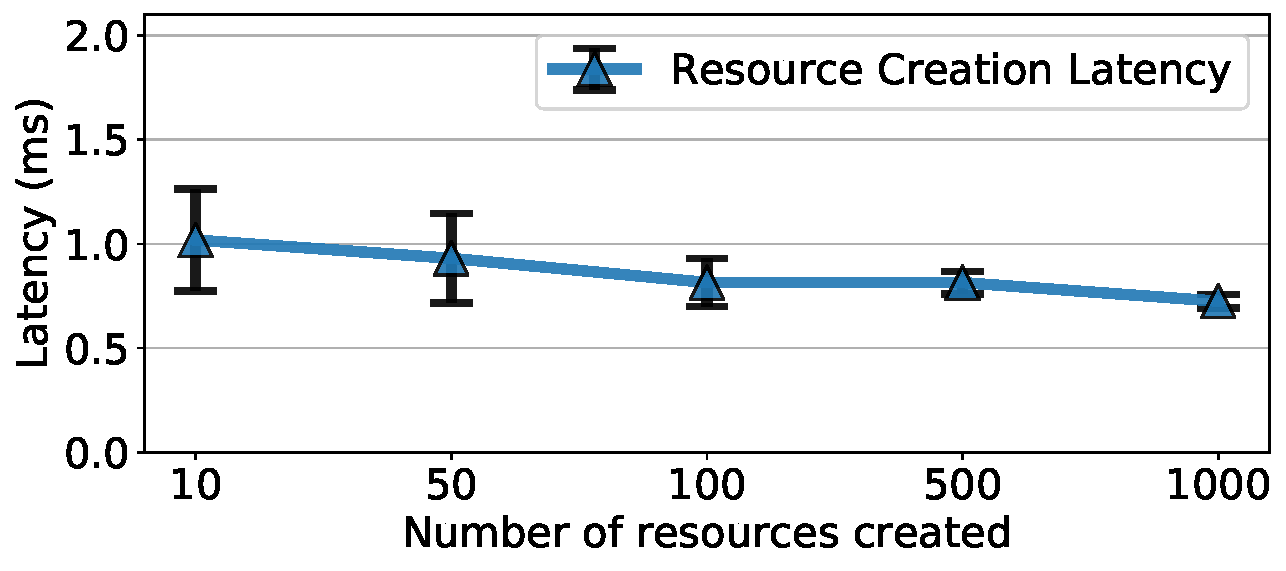
\includegraphics[width=\textwidth]{escher/plots/microbench_horz/result_microbench_creationlatency_vs_numres_horz.pdf}
  \caption{}
  \label{fig:res-creation-microbench}
\end{subfigure}
\begin{subfigure}[b]{0.31\textwidth}
  \centering
  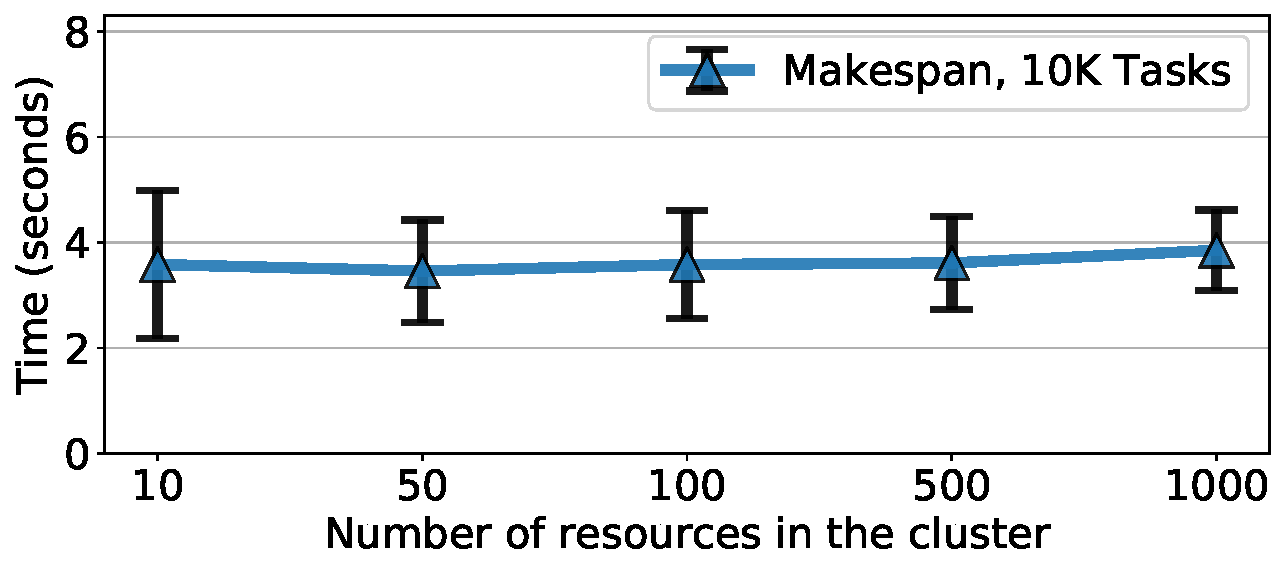
\includegraphics[width=\textwidth]{escher/plots/microbench_horz/result_microbench_schedlatency_vs_clusterresources_horz.pdf}
  \caption{}
  \label{fig:schedlatency-resources-microbench}
\end{subfigure}
\begin{subfigure}[b]{0.31\textwidth}
  \centering
  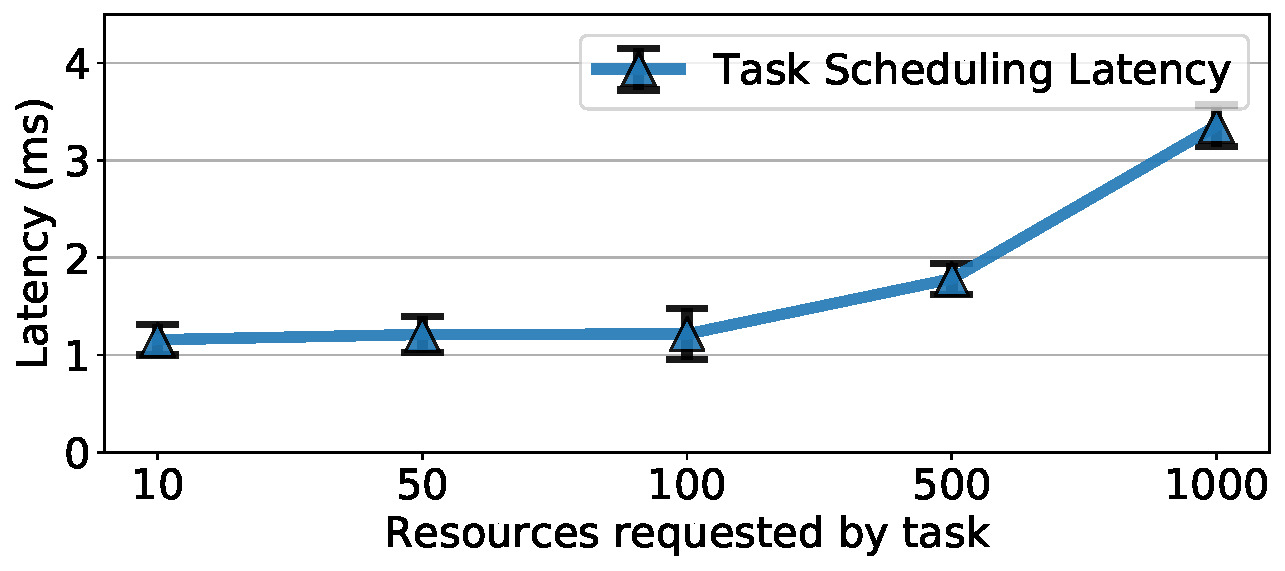
\includegraphics[width=\textwidth]{escher/plots/microbench_horz/result_microbench_schedlatency_vs_resrequested_horz.pdf}
  \caption{}
  \label{fig:schedlatency-taskrequest-microbench}
\end{subfigure}
\vspace{-4mm}
\caption{\small \name{} microbenchmarks. \textbf{(a)} Mean per-resource creation latency in Ray. Creating ephemeral resources in \name{} is a low-cost operation that scales linearly with the number of resources created. \textbf{(b)} Scheduling latency overheads from presence of ephemeral resources. Makespan of a 10000 task workload remains unaffected by the count of ephemeral resources in the cluster. \textbf{(c)} Effect of task resource requirements on scheduling latency in an environment with 10000 resources.}
\label{fig:microbenchfig}
\end{figure*}


\noindent\textbf{Ephemeral resources and scheduling latency.}
%The core task of the framework scheduler is to match task resource requirements with cluster resource availability.
The creation of ephemeral resources may add burden to the scheduler, as it must consider a greater number of attributes during resource matching.
% The usage of ephemeral resources imposes an additional burden on the scheduler and its resource matching complexity, as the number of resource attributes managed by the scheduler and the dimensionality of compared resource attribute vectors grows. 
Therefore, we analyze the effect of resource creation on task scheduling latency. We create an equal number of resources across 50 \ray{} nodes in a cluster using the \lstinline{set_resource} API. We then evaluate two cases based on the resource requirements of the tasks involved.

% \textbf{Tasks without resource requirements.}
First, in Figure~\ref{fig:schedlatency-resources-microbench}, we launch 10,000 tasks, none of which require any ephemeral resources to be scheduled. %, and measure the makespan of this workload against the number of resources present in the cluster.
As the tasks do not have any specific resource requirements, the scheduler execution time and workload makespan are not affected by the number of ephemeral resources present. %, and the makespan of the workload remains unaffected even by the presence of other ephemeral resources in the cluster.

% we highlight the effects of presence of ephemeral resources on scheduling latency for tasks that do not make use of ephemeral resources. In this microbenchmark, we launch a workload of 10k tasks, none of which require any ephemeral resources to be scheduled and compare the makespan of this workload against the number of resources present in the cluster. As the tasks do not have any specific resource requirements, the scheduler execution time remains constant, and the makespan of the workload remains unaffected even by the presence of other ephemeral resources in the cluster.
        % \begin{figure}
        %     \centering
        %     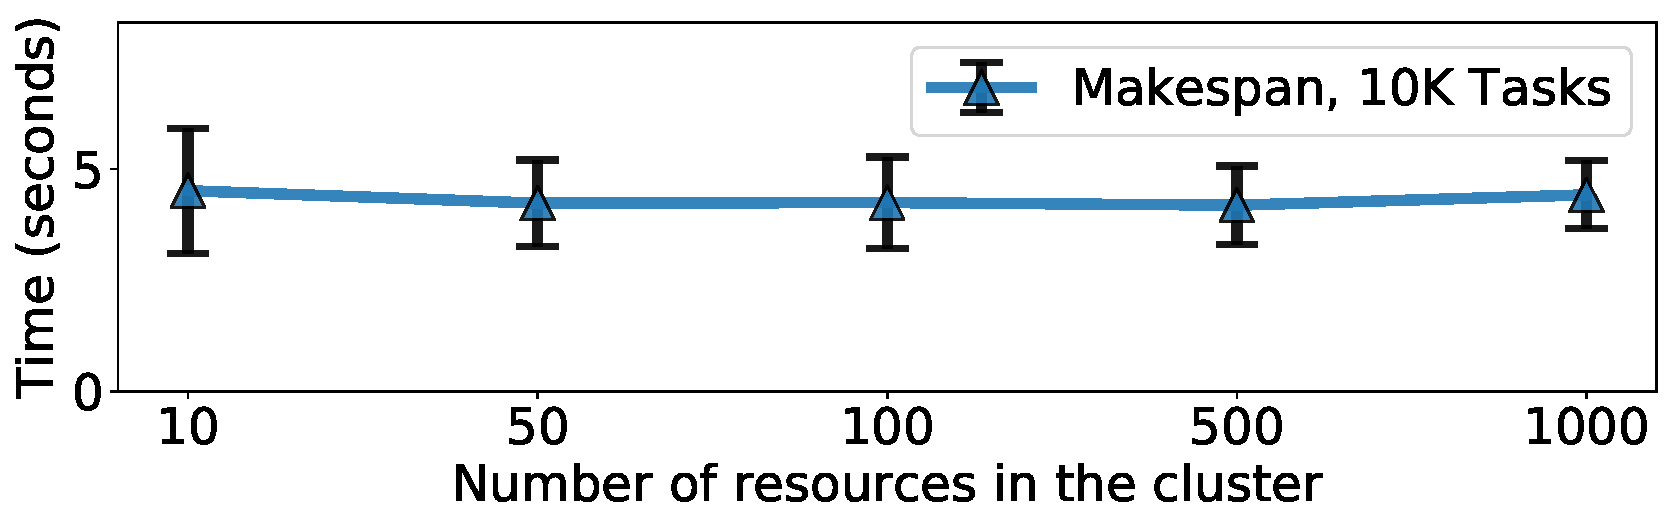
\includegraphics[width=\linewidth]{escher/plots/result_microbench_schedlatency_vs_clusterresources.pdf}
        %     \caption{\small Scheduling latency overheads from presence of ephemeral resources.  The makespan of a  10000 task workload remains unaffected by the count of ephemeral resources present in the cluster. }
        %     \label{fig:schedlatency-resources-microbench}
        %     \vspace{-4mm}
        % \end{figure}
        
% \textbf{Tasks with resource requirements.}
Second, when tasks do request ephemeral resources, the core scheduler must match the task's requirements to a set of candidate nodes.
To evaluate the overheads introduced by this matching, we setup a 50 node \ray{} cluster and create 1000 unique ephemeral resources evenly spread across nodes.
Figure 8c highlights the scalability of the scheduler as the number of ephemeral resources requested by a task grows. The the task scheduling latency grows only from 1.1ms to 1.2ms when requesting 1 vs. 100 ephemeral resources, respectively. We note that all policies described in this work require only a few ephemeral resources to express.
% We then perform multiple trials that launch a no-op task that requests a range from 10 to 1000 distinct resources.
%Figure \ref{fig:schedlatency-taskrequest-microbench} shows the scheduling latency of a no-op task against the number of resource requested by the task. The scheduling latency remains constant up to requests as large as 100 resources. Note that even the most complex scheduling policies do not require more than a few ephemeral resources.
    
        % \begin{figure}
        %     \centering
        %     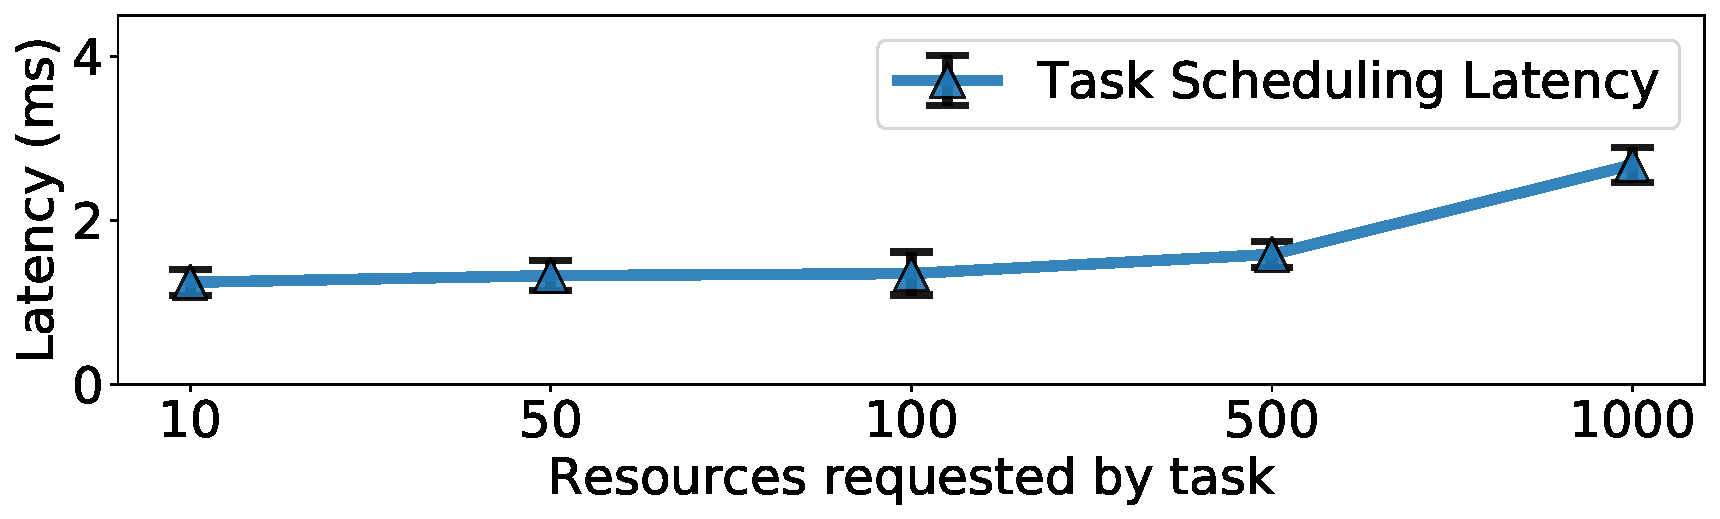
\includegraphics[width=\linewidth]{escher/plots/result_microbench_schedlatency_vs_resrequested.pdf}
        %     \caption{\small Effect of task resource requirements on scheduling latency in an environment with 10000 resources spread over 10 nodes. As a task resource requests more resources, the scheduling latency increases, but even the most complex scheduling policies do not require more than tens of resources. }
        %     \label{fig:schedlatency-taskrequest-microbench}
        % \end{figure}


% \textbf{Value of Locality-Aware scheduling.} In this microbenchmark, we study the motivation for co-location of tasks with the data they operate on. Specifically, we aim to evaluate the network cost of placing tasks and data on separate physical machines. We create arrays of varying sizes across 2 nodes in a \ray{} cluster and run two sets of tasks which fetch the data and perform a no-op. The first set of tasks uses ephemeral resources to co-locate with the data each task works on, while the other set of tasks is randomly placed.

% Figure \ref{fig:locality-latency} compares the task latency when tasks are co-located against random placement. \textcolor{red}{These numbers will be more dramatic soon - this run is local on one machine. Also, Is this a useful microbenchmark?}.

%     \begin{figure}
%         \centering
%         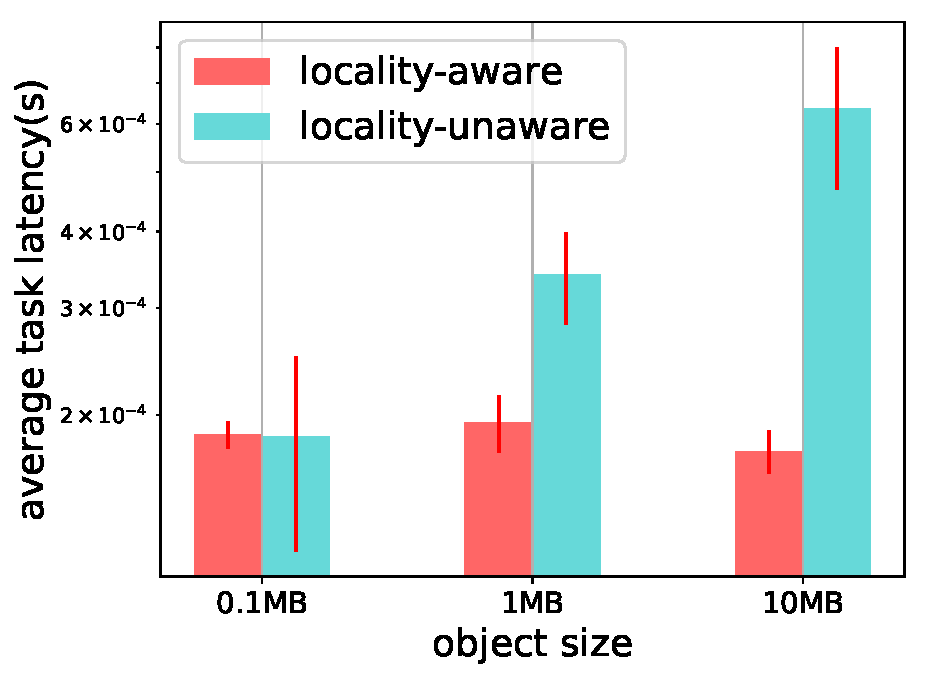
\includegraphics[width=\linewidth]{locality-latency.pdf}
%         \caption{Task-latency - Data-locality vs object size.}
%         \label{fig:locality-latency}
%     \end{figure}

% \subsection{Discussion}
% \textbf{Performance-evolvability tradeoff.} As we implemented our evaluation workloads, we found that \name{} significantly reduced the effort to express the workloads' scheduling constraints. In the AlphaZero workload, it required only 5 lines of code to be changed to express a composition of load-balancing and co-location. Implementing the same policy in Ray would have required re-writing the scheduler to enforce this policy on all tasks, since there is no policy selection mechanism in Ray. Same was true for implementing Gang Scheduling.

% However, as we see in the Gang Scheduling microbenchmark, the ghost task mechanism introduces latency due to the back-off performed by each ghost task on failure. While this latency is insignificant for long-running tasks, such as in distributed training, we acknowledge that this is a natural tradeoff ESCHER makes. It sacrifices performance for certain policies in favor of significantly reducing the implementation burden at the application-level. This gain in evolvability can be valuable for many applications, for whom functionality in the short-term (while the policy is integrated into the scheduler) may be more important than performance. 

% \textbf{Debugging ESCHER policies.} Since ephemeral resources are declarative in nature, debugging them requires replay of resource creation/deletion logs, which can be challenging.

%% \section{Evaluation}
\label{sec:evaluation}

We evaluate \name{} on the Waymo and Cityscapes data. %The highlights are:

\begin{itemize}
    \item With multiple cameras sharing the resources on an edge server, \name{} achieves upto \romilc{16}\% \romil{This is sim, check exact with zhengxu} points higher accuracy than the fair sharing baseline. Attaining the same accuracy with a fair-sharing scheduler would require upto \romilc{$2.xx\times$} more resources.
    \item With the same resource provisioning, \name{} is able to support upto $5\times$ more video streams than the fair scheduler.
    \item \name{}'s performance gracefully degrades with reduction in resources to the baseline that does not retrain since it evaluates the cost of retraining on the accuracy. 
\end{itemize}

\subsection{Methodology}
\label{subsec:eval-setup}

\junchen{need to update}

\noindent\textbf{Datasets.} For our evaluation, we use the Waymo Open\cite{waymo} and Cityscapes\cite{cityscapes} datasets, two popular video datasets containing dashboard camera footage of cars driving through cities in the US and Europe. Cityscapes has frames from 27 video streams training with a total of 5000 pixel-level annotated frames, while Waymo Open has 1000 video segments with a total of 200000 frames.

The workload in Cityscapes is constructed by treating each city's video as an independent video stream feeding into {\name} for inference and retraining. The workload in Waymo Open is constructed by creating video streams by concatenating 20s-video segments belonging to the same city in chronological order. Each video stream in both datasets is then split into 10 retraining windows. These workloads are representative of independent video-streams with local variations which necessitate retraining for their specific data-distributions.



% \noindent\textbf{System Implementation.}\junchen{shrink or remove given the impl section}
% We implement a prototype of \name in Python using Ray\cite{ray} for asynchronous operations and RPCs. 
% Each video stream is modelled as an independent Ray actor whose resource allocation for inference and training is periodically updated by the Ekya master.

% % Write about microprofiling
% %\mypara{Microprofiling}
% The Ekya implementation ingests video streams and splits it into evenly sized retraining periods. At the start of each retraining period, the hyperparameters are micro-profiled \ref{sec:microprofiling} and the thief scheduler is run to compute the resource allocations for training and inference jobs. 
% %This resource allocation is then enforced by Ekya by launching new training processes and restarting the inference processes with updated resource weights. 

% Ekya requires fine-grained GPU allocation between inference and training processes. 
% Talk about memory isolation in Ekya.
% Talk about nvidia MPS resource sharing



\noindent\textbf{Trace driven simulator.}
% \junchen{update this?}
In addition to the system implementation \cref{sec:system}, we also built a simulator to simulate the execution of training and inference jobs under varying resource constraints and workloads. The inputs to the simulator are execution traces from training and inference workloads with different configurations. 

To collect execution traces, we ran all configurations in our hyperparameter space on the 10 retraining windows for every video stream in the Waymo and Cityscapes datasets. For each training job execution in a retraining window, we log the training-accuracy progression over GPU-time. Once the model is trained, we also log its test accuracy over the future retraining windows to get the accuracy in future windows if it was not retrained. This builds an exhaustive trace set that allows us to simulate custom scheduling policies, modify the execution order, simulate resource sharing and allocation. All profiling and trace collection was done on a testbed with Nvidia RTX 2080 and Intel Xeon E-2226G CPU.

% Talk about the assumptions - inference accuracy min GPU, linear scaling etc

\textbf{Hyperparameters.}
For each training job, we create a fixed set of configurations by varying the following hyperparameters - number of epochs to train, batch size, number of neurons in the last layer, number of layers to retrain, and the fraction of data between retraining windows to be used for retraining. We then selected combinations of these hyperparameters to create a diversity in the resource-accuracy profiles of the configurations. 

\mypara{Performance metrics}
\junchen{tbd: accuracy, throughput (\# of streams) under given \# of gpus}

\textbf{Baselines.}
We compare the thief scheduler against a weighted {Fair Scheduler} \cite{fair-1, fair-2, videostorm}, which allocates equal resources to all video streams and within a video stream, allocates resources to training and inference proportional to the weight set as the \lstinline{inference_weight} parameter to scheduler. A higher \lstinline{inference_weight} implies a higher resource allocation to inference and a reduced allocation to training jobs. To pick retraining hyperparameters, the fair scheduler employs the common heuristic of highest-accuracy first. 

%We compare against two baselines. First is \textit{No-retraining}, which does not ever retrain the model and thus allocates resources only to inference. Second is \textit{Fair Scheduler} \cite{fair-1, fair-2, videostorm} which allocates equal resources to all video streams and within a video stream, allocates equal resources to both, training and inference. To pick retraining hyperparameters, the fair scheduler employs the common heuristic of highest-accuracy first. 
% Why are these good baselines?

% \textbf{Metrics.}
% % More:
% Our most used metric is Inference Accuracy over time, as described in \S\ref{subsec:formulation}. We also use the number of GPUs provisioned at the edge server as a measure of cost.


% \junchen{

% 6.2 Overall improvement

% - accuracy vs. gpus (fix \# of videos)

% - streams vs. gpus (fix accuracy)

% - accuracy vs. streams (fix \# of gpus)

% - alternative architectures



% 6.3 Understanding Ekya improvements

% - ablation analysis

% - per-stream gains

% - temporal behaviors



% 6.4 Microbenchmarking

% - estimation accuracy of microprofiling

% - impact of microprofiling erros

% - delay of thief scheduler

% - impact of scheduling granularity


% }

% overall improvement: 
% acc vs gpu
% mention the cloud baseline
\subsection{Overall improvements}

\begin{figure}
  \centering
%   \begin{subfigure}[t]{0.5\linewidth}
%     \centering
%     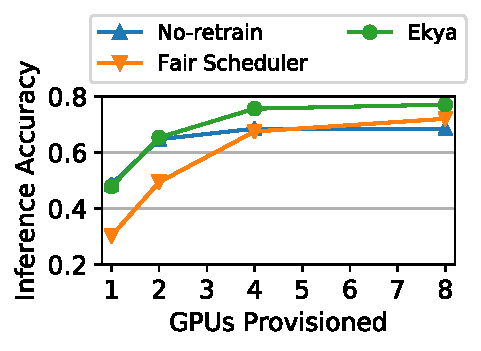
\includegraphics[width=\linewidth]{results/multicam/multicam_acc_vs_res_cityscapes.pdf} 
%     \caption{Cityscapes}
%     \label{fig:scalability-gpus-cityscapes}
%   \end{subfigure}
%   ~~~
%   \begin{subfigure}[t]{0.5\linewidth}
%     \centering
%     % \includegraphics[width=\linewidth]{figures/motivation/Class_Incrementality/class_distribution_change_sf_27.png}
%     \includegraphics[width=\linewidth]{results/multicam/multicam_acc_vs_res_waymo.pdf}
%      \caption{Waymo}
%     \label{fig:scalability-gpus-waymo}
%   \end{subfigure}
  \begin{subfigure}[t]{0.5\linewidth}
    \centering
    \includegraphics[width=\linewidth]{results/multicam/cityscapes_across_resources.pdf} 
    \caption{Cityscapes}
    \label{fig:scalability-gpus-cityscapes-golden}
  \end{subfigure}
  ~~~
  \begin{subfigure}[t]{0.5\linewidth}
    \centering
    \includegraphics[width=\linewidth]{results/multicam/waymo_across_resources.pdf} 
    \caption{Waymo}
    \label{fig:scalability-gpus-waymo-golden}
  \end{subfigure}
  \caption{\bf Multi-video performance: Our accuracy gain over baselines increases with more GPUs. \romil{Set x,y axis labels and use the custom size params for matplotlib formatting. Reviewer Q.: How do you partition 10 video streams over 8 GPUs?}}
  \label{fig:scalability-gpus}
\end{figure}

\mypara{Accuracy vs. provisioned resource}
Figure~\ref{fig:scalability-gpus} compares the performance of \name, average inference accuracy under same amount of total GPU resource, with the no-retraining baseline and the fair-scheduler baseline.
In each of the Waymo and Cityscapes traces, we randomly pick 10 video streams and run their inference concurrently through five retraining windows.
As we increase the number of provisioned GPUs, we see that \name consistently outperforms the best of the two baselines by a considerable margin
\romilc{xx}\%-\romilc{xx}\% points higher accuracy in Cityscapes and \romilc{xx}\%-\romilc{xx}\% points in Waymo.
Note that these gains in accuracy are achieved without increasing inference delay.
\name allocates resource to retraining only when the accuracy gain from retraining the model outweighs the temporary accuracy drop due to frame subsampling, which explains why \name outperforms the no-retraining baseline. 
Moreover, when \name allocates resource to retraining, it allocates minimum amount needed by the retraining to finish in time, thus outperforming the fair scheduler.
While accuracy gap between \name{} and the fair scheduler baseline decreases as more GPUs are provisioned, \name needs much less resources (upto $6.5\times$ less GPUs, Table \ref{tab::resource-savings-golden}) to achieve the maximum accuracy that fair scheduler attains with 8 GPUs.

%\name's gains over no-retrain baseline are more sizable in Waymo than Cityscapes, but its gains over the fair scheduler baseline are comparable in both traces. 
%This suggests that Waymo data is inherently more suitable for continuous retraining, but through more intelligent resource allocation, \name can always squeeze more juice from retraining than fair scheduler.



% 
\begin{table}[t]
\small
\begin{tabular}{|c|c|c|c|c|}
\hline
\multirow{2}{*}{\begin{tabular}[c]{@{}c@{}}Video\\ Stream\end{tabular}} & \multirow{2}{*}{Accuracy} & \multicolumn{2}{c|}{GPUs Required} & \multirow{2}{*}{\begin{tabular}[c]{@{}c@{}}Resource\\ Savings\end{tabular}} \\ \cline{3-4}
                                                                        &                           & Ekya        & Fair Scheduler       &                                                                             \\ \hline
V0                                                                      & 76.6\%                    & 4           & 13.4                 & $3.3\times$                                                                 \\ \hline
V1                                                                      & 91.5\%                    & 4           & 4.9                  & $1.2\times$                                                                 \\ \hline
V2                                                                      & 78.1\%                    & 4           & 11.2                 & $2.8\times$                                                                 \\ \hline
V3                                                                      & 68.5\%                    & 4           & 14.9                 & $3.7\times$                                                                 \\ \hline
V4                                                                      & 66.9\%                    & 4           & 17.2                 & $4.3\times$                                                                 \\ \hline
V5                                                                      & 81\%                      & 4           & 6.4                  & $1.6\times$                                                                 \\ \hline
V6                                                                      & 80.9\%                    & 4           & 9.4                  & $2.3\times$                                                                 \\ \hline
V7                                                                      & 76.8\%                    & 4           & 15.1                 & $3.7\times$                                                                 \\ \hline
V8                                                                      & 67.8\%                    & 4           & 14.2                 & $3.5\times$                                                                 \\ \hline
V9                                                                      & 67.9\%                    & 4           & 8.9                  & $2.2\times$                                                                \\ \hline
\end{tabular}
\caption{Resource savings for different cities in Cityscapes.}
\label{tab:resource-savings-final}
\end{table}

\begin{table}[t]
\small
\begin{tabular}{|c|c|c|c|c|}
\hline
\multirow{2}{*}{\begin{tabular}[c]{@{}c@{}}Video\\ Stream\end{tabular}} & \multirow{2}{*}{Accuracy} & \multicolumn{2}{c|}{GPUs Required} & \multirow{2}{*}{\begin{tabular}[c]{@{}c@{}}Resource\\ Savings\end{tabular}} \\ \cline{3-4}
                                                                        &                           & Ekya        & Fair Scheduler       &                                                                             \\ \hline
V0                                                                      & 75.6\%                    & 4           & 15.6                 & $3.9\times$                                                                 \\ \hline
V1                                                                      & 78.6\%                    & 4           & 10.0                  & $2.5\times$                                                                 \\ \hline
V2                                                                      & 76.5\%                    & 4           & 19.5                 & $4.9\times$                                                                 \\ \hline
V3                                                                      & 74.5\%                    & 4           & 17.4                 & $4.4\times$                                                                 \\ \hline
V4                                                                      & 75.1\%                    & 4           & 20.9                 & $5.2\times$                                                                 \\ \hline
V5                                                                      & 71.4\%                      & 4           & 25.8                  & $6.5\times$                                                                 \\ \hline
V6                                                                      & 79.5\%                    & 4           & 8.05                  & $2.0\times$                                                                 \\ \hline
V7                                                                      & 75.3\%                    & 4           & 21.8                 & $5.5\times$                                                                 \\ \hline
V8                                                                      & 75.0\%                    & 4           & 84.5                 & $21.1\times$                                                                 \\ \hline
V9                                                                      & 75.2\%                    & 4           & 177.8                  & $44.5\times$                                                                \\ \hline
\end{tabular}
\caption{\bf\small Resource savings for different cities in Cityscapes. \romil{We should write DNF for V7 V8 V9. \romil{This is a bit confusing because every row is not running independently - so this isn't  per resource saving. We should either get overall aggregate number here or run V0 repeatedly to get per video number.}}}
\label{tab:resource-savings-golden}
\end{table}
% gains per stream
\mypara{Performance per video stream}
Figure~\ref{fig:multicam-cities} shows the improvements {\em per video stream} of \name over the baselines, using the same 10 video streams as in Figure~\ref{fig:scalability-gpus} when 4 GPUs provisioned. 
Rather than trading accuracies among video streams, \name re-allocates resources in a way that improves accuracy for {\em all} of the video streams. 
That said, the accuracy gain varies, with gains being more considerable on video streams that have low accuracy without retraining (no-retraining).
This is because these video streams tend to have more dynamic scenes thus may benefit more from retraining.
This highlights a desirable behavior of \name that resource will more likely to be assigned where more accuracy gains are expected.
% \junchen{again, any insight as to what might cause the difference between the two traces?}



% % temporal variance
% \mypara{Timeseries of \name performance}
% Figure~\ref{fig:multicam-timeseries} zooms in on one of the video streams from Figure~\ref{fig:multicam-cities} (V\fillme) and presents the timeseries of performance of \name and the baselines over the five retraining windows. 
% This is one of the video streams that see a high accuracy gain over no-retraining. 
% The timeseries corroborates our intuition: when no-retraining accuracy is low (the \fillme-th retraining window), \name allocates resource to allow it to retrain its model which keeps the accuracy at a high value.

% \begin{figure}
% 	\includegraphics[width=0.4\textwidth]{results/multicam/multicam_taskwise_acc_zurich_4_cityscapes.pdf}
% 	\caption{\bf Timeseries of our performance vs. fair sharing. Again, adaptive resource sharing constantly outperforms fair sharing. \romil{Accuracy drops over time.}}
% 	\label{fig:multicam-timeseries}
% \end{figure}


% scalability: with more gpus, we can support more camera
\mypara{Scalability with more GPUs}
Next, we evaluate the scalability of \name's {\em throughput} as more GPUs are available.
We define throughput as the maximum number of video streams that can run concurrently on the GPUs while achieving a accuracy within a threshold of the maximum possible mean accuracy.
(This definition is common in practice, since applications usually require accuracy to be above a threshold for the inference to be usable.)
Figure~\ref{fig:scalability-gpu-vs-cam-thresholded} shows that \name's throughput grows almost linearly with more available GPUs, and at a rate \romilc{$2.3\times$} faster than the baseline of fair scheduler.
This suggests that \name can more easily scale to a large number of video sources than the baselines.

\begin{figure}
  \centering
%   \begin{subfigure}[t]{\linewidth}
%     \centering
%     \includegraphics[width=0.9\linewidth]{results/multicam/multicam_individual_stream_acc_cityscapes.pdf} 
%     \caption{Cityscapes Human Label}
%     %\label{fig:multicam-cities-cityscapes}
%   \end{subfigure}
    \begin{subfigure}[t]{\linewidth}
    \centering
    \includegraphics[width=0.9\linewidth]{results/multicam/cityscapes_across_cities.pdf} 
    %\caption{Cityscapes Golden Model}
    %\label{fig:multicam-cities-cityscapes}
  \end{subfigure}
%   ~~~
%   \begin{subfigure}[t]{0.5\linewidth}
%     \centering
%     % \includegraphics[width=\linewidth]{figures/motivation/Class_Incrementality/class_distribution_change_sf_27.png}
%     \includegraphics[width=\linewidth]{results/multicam/multicam_individual_stream_acc_waymo.pdf}
%      \caption{Waymo}
%     \label{fig:multicam-cities-waymo}
%   \end{subfigure}
  \caption{Multi-video performance: Ours (with continuous retraining) vs. Fair Share Scheduler. Compared across cities, we do consistently better. Some cities see bigger gains than others, which are thus prioritized by \name{}.}
  \label{fig:multicam-cities}
\end{figure}


Figure \ref{fig:scalability-fixedGPUs-accuracy} evaluates the throughput-accuracy tradeoff made by \name{} with a fixed number of resources. To minimize the accuracy variations between cities, we add video streams by replicating a fixed video stream from the Cityscapes dataset. 
With only a single GPU, increasing the number of video streams forces \name{} to gradually reduce resource allocation to retraining in favour of keeping of a high inference accuracy by allocating all resources to inference. The fair scheduler is unaware of the resource cost of retraining, and diverts GPU cycles from inference, resulting a lower inference accuracy.

\begin{figure}
 	%\includegraphics[width=0.4\textwidth]{figures/eval_placeholders/single-tradeoffs.pdf}
 	\includegraphics[width=\linewidth]{results/scalability/scalability_GPUs_cams_cityscapes.pdf}
	\caption{\bf Throughput measured as number of video streams that can be concurrently supported for different resource sizes subject to accuracy thresholds.
	%The accuracy threshold is a multiplicative factor of the maximum achievable mean accuracy for a workload given $\infty$ resources.
	}
	\label{fig:scalability-gpu-vs-cam-thresholded}
\end{figure}

% SIGCOMM Results:
% \begin{figure}
%  	%\includegraphics[width=0.4\textwidth]{figures/eval_placeholders/single-tradeoffs.pdf}
%  	\includegraphics[width=\linewidth]{results/scalability/scalability_cams_fixedGPUs_cityscapes.pdf}
% 	\caption{\bf Effect of adding more video streams on accuracy for different schedulers. When insufficient resources are provisioned, \name{} gracefully degrades to the No-retrain baseline, while the retraining decisions made by the fair scheduler reduce the mean inference accuracy.}
% 	\label{fig:scalability-fixedGPUs-accuracy}
% \end{figure}
\begin{figure}
 	%\includegraphics[width=0.4\textwidth]{figures/eval_placeholders/single-tradeoffs.pdf}
 	\includegraphics[width=\linewidth]{results/scalability/scalability_cams_fixedGPUs_cityscapes_golden_model.pdf}
	\caption{\bf Using golden model. Effect of adding more video streams on accuracy for different schedulers. When insufficient resources are provisioned, \name{} gracefully degrades to the No-retrain baseline, while the retraining decisions made by the fair scheduler reduce the mean inference accuracy.}
	\label{fig:scalability-fixedGPUs-accuracy}
\end{figure}


% per video. even if one video, gains are impressive
\mypara{Gains with single video stream}
Figure~\ref{fig:singlecam-cities} presents the same analysis of Figure~\ref{fig:scalability-gpus} but with only one video stream using the resources.
Across these video streams (and many others but not shown), we see that \name consistently outperforms the baselines by dynamically deciding when to retrain the model as well as the resource balance between retraining and inference.
As in Figure~\ref{fig:multicam-cities}, we see the gains vary considerably across video streams, which again highlights that some video streams can inherently benefit more from retraining.% their models.

% \begin{figure}
%   \centering
%   \begin{subfigure}[t]{\linewidth}
%     \centering
%     \includegraphics[width=\linewidth]{results/singlecam/singlecam_acc_vs_cost_cityscapes.pdf} 
%     \caption{Cityscapes}
%     \label{fig:singlecam-cities-cityscapes}
%   \end{subfigure}
%   \hfill
%   \begin{subfigure}[t]{\linewidth}
%     \centering
%     \includegraphics[width=\linewidth]{results/singlecam/singlecam_acc_vs_cost_waymo.pdf}
%     \caption{Waymo}
%     \label{fig:singlecam-cities-waymo}
%   \end{subfigure}
%   \caption{Single-video performance - different videos have different payoffs for retraining.}% In \ref{fig:singlecam-cities-cityscapes}, V2 demonstrates large benefits to retraining compared to V4.}
%   \label{fig:singlecam-cities}
% \end{figure}

\begin{figure}
  \centering
  \begin{subfigure}[t]{\linewidth}
    \centering
    \includegraphics[width=\linewidth]{results/singlecam/singlecam_acc_vs_cost_golden_cityscapes.pdf} 
    \caption{Cityscapes}
    \label{fig:singlecam-cities-cityscapes-golden}
  \end{subfigure}
  \hfill
  \begin{subfigure}[t]{\linewidth}
    \centering
    \includegraphics[width=\linewidth]{results/singlecam/singlecam_acc_vs_cost_golden_waymo.pdf}
    \caption{Waymo}
    \label{fig:singlecam-cities-waymo-golden}
  \end{subfigure}
  \caption{Single-video performance - different videos have different payoffs for retraining.}% In \ref{fig:singlecam-cities-cityscapes}, V2 demonstrates large benefits to retraining compared to V4.}
  \label{fig:singlecam-cities}
\end{figure}


\subsection{Comparison with alternative designs}
\label{subsec:eval-alternate}

Next, we evaluate two alternative designs for continuous retraining---(1) re-using a retrained model from a history window that shares class distribution (instead of retraining the model again) and (2) offloading the retraining to the cloud.

\mypara{Advantage over re-using cached models}
Reusing a cached model from history is tempting as it avoids the cost of model retraining. 
%Figure~\ref{fig:history-vs-current} compares 
We compare the accuracy of retraining the model on the current window (\name) with the accuracy of re-using the model from a history window in which the class distribution is close to the distribution in the current window (Euclidean distance $\leq 0.2$; \S\ref{sec:profiling}). Here we use ResNet18 as the model and Waymo as the trace.
%The graph, however, shows 
We observe that 
the accuracy is much lower by re-using the model from history, even when the history window share a similar class distribution. At median, the difference in accuracy is 11\% with the $90^\text{th}$ percentile and maximum divergence in accuracies being as high as $38\%$ and $51\%$. 
This confirms our intuition in \S\ref{sec:profiling} that although sharing a similar class distribution is indicative of the difficulty of retraining, it does not mean the model can be directly reused from any window with similar class distribution.


%\begin{figure}[t!]
%\centering
%\includegraphics[width=0.6\columnwidth]{figures/eval_placeholders/history-trained-vs-retrained-cdf.pdf}
%\vspace{-0.2cm}
%\caption{Gap between accuracy of the model retrained in the current and accuracy of re-using a model retrained in a history window that share similar class distribution.
%\vspace{-0.2cm}}
%\label{fig:history-vs-current}
%\end{figure}


\mypara{Advantage over a cloud-based solution}
Retraining could be offloaded to the cloud so the edge servers can focus on inference, but on a closer look such a cloud-based solution will even negate the benefit of retraining the model, because of the expensive communication delay from uploading training data to the cloud and downloading retrained models). 

%It is fundamentally challenging to run continuous learning across the edge-cloud because of network constraints.

% Math sheet new - https://docs.google.com/spreadsheets/d/1-WDeFmQwHy0sEpxL9f6QcbMKt1DVPaX6ODjMwDbb3IY/edit#gid=0
For instance, consider a setup serving 5 video streams in parallel with a retraining window size of 400 seconds. For a bit rate of 8 Mbps \cite{bitrate} and assuming a 10\% subsampling, it amounts to 320 Mb of training data being generated per camera in every retraining window. This retraining data must be uploaded to cloud and a model must be retrained and fetched back to the edge. Uploading 320 Mb over an average cellular uplink of 5.1 Mbps \cite{opensignal_2018} for 5 cameras results in a total upload time of 313 seconds. A model checkpoint of ResNet18 is 398 Mb, downloading which would take 23 seconds per camera on a downlink of 17.3 Mbps \cite{opensignal_2018}, or a total of 115 seconds for 5 cameras. The total network transfer cost is 428 seconds, which exceeds the retraining window size of 400 seconds. 

% Mention do we have to send everything to the cloud.

% examples where the drop is higher
Even on provisioning double the bandwidth (which entails an expensive change of the network link from cellular to cable), retraining on the cloud does not yield a higher accuracy in our simulator. We extend our simulator to simulate the network delays and assume that the the cloud offers a speed up of $10\times$ and has infinite parallel resources. Even then, the cloud \romilc{RTT} takes about 216 seconds and yields a mean inference accuracy of 81.8\%. In contrast, retraining at the edge completes in 125 seconds, leaving more time to take advantage of the retraining model, and results in an inference accuracy of 83.75\%.

% Show the calculation
% Mention the cost
% Varying network connections
Achieving the same accuracy in our simulations required increasing the downlink and uplink bandwidth by $3\times$ and still operates under the assumption that the cloud can provision parallel resources instantly, which can be expensive.

% Math sheet- https://docs.google.com/spreadsheets/d/1z4Zui8Qmg4iH-_yQKu7p0EZtXOlj_-ogKIW9mbf-Tpo/edit#gid=179811194

% For instance, each retraining window in the Waymo dataset accumulates about 1760 Mb of data every 20 seconds, resulting in a 88 Mb/s bitrate. Assuming a 10\% sub-sampling rate for retraining and a retraining window of 200 seconds (as in all our experiments), a total of 1760 Mb  of training data must be sent to the cloud. With an uplink of 5.1 Mb/s \cite{opensignal_2018}, just uploading the training data would take 345 seconds. Moreover, the updated model weights need to be downloaded from the cloud, which is 360 Mb in size. With a downlink throughput of 17.3 Mb/s \cite{opensignal_2018} (cellular connection), that adds another 20 seconds. Combined, this results in nearly 365s to get the retrained model, which far exceeds the retraining window size of 5 minutes (note that we have ignored the time to run the training in the cloud). Since even the sub-sampled video bitrate exceeds the limited bandwidths at the edge, this analysis applies for all retraining window sizes.


% \junchen{i still feel this should be in motivation section, no?}

\subsection{Sensitivity analysis}
\label{subsec:sensitivity-eval}

% \begin{figure} [t!]
%  	%\includegraphics[width=0.4\textwidth]{figures/eval_placeholders/single-tradeoffs.pdf}
%  	\includegraphics[width=\linewidth]{results/ablation_waymo.pdf}
% 	\caption{\bf {\name} factor analysis by removing  dynamic resource allocation and reducing the hyperparameter space.}
% 	\label{fig:factor-analysis}
% \end{figure}

\begin{figure} [t!]
 	%\includegraphics[width=0.4\textwidth]{figures/eval_placeholders/single-tradeoffs.pdf}
 	\includegraphics[width=\linewidth]{results/ablation_cityscapes_golden.pdf}
	\caption{\bf {\name} factor analysis by removing  dynamic resource allocation and reducing the hyperparameter space.}
	\label{fig:factor-analysis}
\end{figure}

% improvement breakdown
\mypara{Factor analysis}
To understand the contribution of each part of \name, we run a factor analysis on the same setting as Figure~\ref{fig:scalability-gpus} (10 video streams with 4 GPUs provisioned). We construct two schedulers from {\name}. \emph{Ekya-NoRes}, which removes the smart resource allocation in \name. \emph{Ekya-NoRes-NoEp} removes resource allocation and additionally fixes the number of epochs a model is trained to the maximum value, effectively removing it from the configuration space. We chose this hyperparameter for removal because it creates the largest diversity in the resource-accuracy profiles of configurations. 

As observed in Figure \ref{fig:factor-analysis}, the diversity in configurations and their careful selection has a large contribution to \name{}'s gains in accuracy when fewer resources are provisioned, which reduces as more resources are made available. This is because with more resources, even expensive configurations become feasible, thus configuration selection matters less. The smart resource allocation mechanism in {\name} has a nearly consistent contribution to \name{}'s performance.

%We note that the accuracy of \emph{Ekya-NoRes-NoEp} is lower than \emph{No-retrain} when 1 GPU is provisioned because resource reallocation is removed, and thus it always allocates resources to retraining. It just so happens that there are no good configurations to pick from once the epochs hyperparameter is removed, and thus the accuracy is lesser than \emph{No-retrain}.



% sensivity to accuracy errors
\mypara{Sensitivity to accuracy estimation errors}
\romil{Add paragraph and plot on accuracy of microprofiling.} %Resource consumption and accuracy of accuracy estimation. E
We now test the impact of errors in accuracy profiles (\S\ref{subsec:profiling}) on \name's performance gains.
To control the amount of errors, we add a controlled Gaussian noise on top of the real retraining accuracy as the predictions when the profiler is queried. 
Figure~\ref{fig:sensitivity-accuracy-error} shows that with upto 20\% errors in the profiler prediction, the maximum accuracy drop is 3\% points. When a 50\% profiling error is introduced, the accuracy drop is 7.9\% points. Such a large profiling error makes \name{} worse than the no-retrain baseline, but still better than fair scheduling.

\begin{figure}
	\includegraphics[width=\linewidth]{results/sensitivity/sensitivity_profileerrors_cityscapes.pdf}
	\caption{\bf Adding a controlled error $\epsilon$ to the accuracy prediction -  \name{}'s performance degrades, but only marginally.}
	\label{fig:sensitivity-accuracy-error}
\end{figure}

% Two subfigure plot for sensitivity 
% \begin{figure}
%   \centering
%   \begin{subfigure}[t]{0.5\linewidth}
%     \centering
%     \includegraphics[width=\linewidth]{results/sensitivity/sensitivity_profileerrors_cityscapes.pdf} 
% 	\caption{\bf Adding errors to the profiler.}
%     \label{fig:sensitivity-accuracy-error}
%   \end{subfigure}
%   ~~~
%   \begin{subfigure}[t]{0.5\linewidth}
%     \centering
%     % \includegraphics[width=\linewidth]{figures/motivation/Class_Incrementality/class_distribution_change_sf_27.png}
%     \includegraphics[width=\linewidth]{results/sensitivity/sensitivity_delta_acc_runtime_cityscapes_48gpu.pdf}
%      \caption{Effect of stealing parameter $\delta$ on the thief scheduler.}
%     \label{fig:sensitivity-delta}
%   \end{subfigure}
%   \caption{\bf Sensitivity Analysis Results.}
%   \label{fig:sensitivity-group}
% \end{figure}

% sensitivity to granularity
\mypara{Sensitivity to scheduling granularity} \ga{Change $\delta$ to $\Delta$ in the graphs and text.}
Finally, we show the sensitivity of \name to the allocation quantum $\delta$ (Algorithm \ref{algo:thief_sched}), which controls the runtime of the scheduling algorithm on the one hand and the result of the resource allocation on the other.
Figure~\ref{fig:sensitivity-delta} illustrates this tradeoff with the same setting as Figure~\ref{fig:scalability-gpus} (10 video streams with 4 or 8 GPUs provisioned).
Between $\delta=0.1$ and 1.0, higher $\delta$ reduces the runtime of the scheduler by 4$\times$, but the accuracy gain is severely affected. 
One should pick a higher $\delta$ only when the scheduler is relatively slow compared to a retraining window; otherwise, a low value of $\delta$ (fine-grained scheduling) is preferable.

\begin{figure}
  \centering
  \begin{subfigure}[t]{\linewidth}
    \centering
    \includegraphics[width=\linewidth]{results/sensitivity/sensitivity_delta_acc_runtime_cityscapes_48gpu.pdf}
  \end{subfigure}
  \caption{\bf Effect of the $\delta$ parameter on the thief scheduler. Larger values decrease the accuracy but are faster to compute.}
  \label{fig:sensitivity-delta}
\end{figure}

\subsection{System Implementation}
\romil{WIP}
\romil{Move this up in the implementaiton section and start with this result.}
The Ekya implementation is an end-to-end system which can ingest video streams and distribute retraining and inference jobs over a pool of shared GPU resources. We ran this implementation on our Edge test-bed \ref{machine-specs}. The load on the system was varied by changing the number of video streams that must be processed in parallel on the same pool of resources. \cref{fig:sysimpl-result} illustrates the performance of Ekya comapred against the fair scheduler for Cityscapes and Waymo datasets. Ekya offers a consistently higher accuracy than the fair baseline (by upto 8\% points) and Ekya can achieve the same accuracy as the fair scheduler, but support $2\times$ the number of video streams in parallel on the same set of resources.

Ekya's performance is affected by the runtime efficiency of it's scheduler. The thief scheduler's search over the resource-configuration space \ref{algo:thief_sched} can be computationally expensive, but relative to retraining window size, it is a small cost. As shown in \Cref{fig:sensitivity-schedlatency}, the t  hief scheduler computes a resource allocation for a retraining window of 200 seconds even when multiple GPUs must be allocated.

\begin{figure}
  \centering
  \begin{subfigure}[t]{\linewidth}
    \centering
    \includegraphics[width=\linewidth]{results/sensitivity/scheduler_resourcetime.pdf}
  \end{subfigure}
  \caption{\bf Thief scheduler latency for scheduling 10 video streams with varying available resource quantities and retraining period durations. The scheduler latency is a tiny fraction compared to the duration of the retraining period.  }
  \label{fig:sensitivity-schedlatency}
\end{figure}


\begin{figure}
  \centering
  \begin{subfigure}[t]{0.5\linewidth}
    \centering
    \includegraphics[width=\linewidth]{results/sys_impl/multicam_acc_vs_res_sysimpl_cityscapes.pdf} 
    \caption{Cityscapes}
    \label{fig:sysimpl-result-cityscapes}
  \end{subfigure}
  ~~~
  \begin{subfigure}[t]{0.5\linewidth}
    \centering
    \includegraphics[width=\linewidth]{results/sys_impl/sysimpl_varyingcities_waymo.pdf} 
    \caption{Waymo}
    \label{fig:sysimpl-result-waymo}
  \end{subfigure}
  \caption{\bf End-to-end accuracy on the system implementation on 1 GPU with varying number of cities.}
  \label{fig:sysimpl-result}
\end{figure}
\section{Implementation and Experimental Setup}
\label{subsec:eval-setup}

% \junchen{need to update}

\mypara{Implementation}
\name uses PyTorch~\cite{pytorch} for running and training ML models, and each component is implemented as a collection of long-running processes with the Ray\cite{ray} actor model. The micro-profiler and training/inference jobs run as independent actors which are controlled by the thief scheduler actor. \name achieves fine-grained and dynamic reallocation of GPU between training and inference processes using Nvidia MPS~\cite{nvidia-mps}, which provides resource isolation within a GPU by intercepting CUDA calls and rescheduling them. Our implementation also adapts to errors in profiling by reactively adjusting its allocations if the actual model performance diverges from the predictions of the micro-profiler. \name's code and datasets are available at the project page: \href{https://aka.ms/ekya}{aka.ms/ekya}

\mypara{Datasets} 
We use both on-road videos captured by dashboard cameras as well as urban videos captured by mounted cameras. The dashboard camera videos are from cars driving through cities in the US and Europe, Waymo Open~\cite{waymo} (1000 video segments with in total 200K frames) and Cityscapes~\cite{cityscapes} (5K frames captured by 27 cameras) videos. The urban videos are from stationary cameras mounted in a building (``Urban Building'') as well as from five traffic intersections (``Urban Traffic''), both collected over 24-hour durations. % and a set of 24-hour urban traffic videos (``Urban Traffic'') captured by 5 cameras. %\junchen{add bellevue dataset once it's included}
% For our evaluation, we use the Waymo Open\cite{waymo} and Cityscapes\cite{cityscapes} datasets, two popular video datasets containing dashboard camera footage of cars driving through cities in the US and Europe. Cityscapes has frames from 27 video streams training with a total of 5000 pixel-level annotated frames, while Waymo Open has 1000 video segments with a total of 200000 frames.
We use a retraining window of 200 seconds in our experiments, and split each of the videos into 200 second segments.  
%The traffic videos are captured continuously and we split them into 200-second retraining windows. 
Since the Waymo and Cityscapes dataset do not contain continuous timestamps, we 
%However, the two public datasets %organize their images chronologically but 
%do not contain continuous timestamps.We 
create retraining windows by concatenating images from the same camera in chronological order to form a long video stream and split it into 200 second segments. %10 retraining windows. 
% in Cityscapes, treating a block of consecutive \fillme images from the same video source (in total 27 sources); and (2) in Waymo, concatenating 20s-video segments belonging to the same source in chronological order.
% The workload in Cityscapes is constructed by treating each city's video as an independent video stream feeding into {\name} for inference and retraining. The workload in Waymo Open is constructed by creating video streams by concatenating 20s-video segments belonging to the same city in chronological order. Each video stream in both datasets is then split into 10 retraining windows. 
%%GA While these images may not be captured at a uniform interval over time, they show representative workloads of independent video streams with local variations which necessitate retraining for their specific data-distributions.


% \mypara{DNN models}
% \revtext{
% We evaluate \name{} on two separate machine learning tasks - object classification and object detection. Our experiments run on a diverse set of edge DNNs - ResNet18\cite{deepresidual-2}, MobileNetV2\cite{compression-17} and SqueezeNet\cite{compression-18} for object classification and TinyYOLOv3\cite{redmon2018yolov3} and SSD\cite{liu2016ssd} for object detection. As explained in \S\ref{subsec:continuous}, we use an expensive golden model (ResNeXt 101 \cite{wang2019elastic} for object classification and YOLOv3 \cite{redmon2018yolov3} for object detection.) to get ground truth labels for training and testing.
% %The golden model-produced labels are also used as ground truth to evaluate inference accuracy.
% On a subset of data that have human annotations, we confirm that the labels produced by the golden model are very similar to human-annotated labels.} %\romil{Golden model acc Cityscapes: 82\% Waymo: 76\%}
% % \junchen{add golden model labeling and that golden model cannot run on every image}

\revtext{
\mypara{DNNs}
We demonstrate \name's effectiveness on two machine learning tasks -- object classification and object detection -- using multiple compressed edge DNNs for each task:
$(i)$ object classification using ResNet18\cite{deepresidual-2}, MobileNetV2\cite{compression-17} and ShuffleNet\cite{shufflenet}, and $(ii)$ object detection using TinyYOLOv3\cite{redmon2018yolov3} and SSD\cite{liu2016ssd}. As explained in \S\ref{subsec:continuous}, we use an expensive golden model (ResNeXt 101 \cite{wang2019elastic} for object classification and YOLOv3 \cite{redmon2018yolov3} for object detection) to get ground truth labels for training and testing.}


% \noindent\textbf{System Implementation.}\junchen{shrink or remove given the impl section}
% We implement a prototype of \name in Python using Ray\cite{ray} for asynchronous operations and RPCs. 
% Each video stream is modelled as an independent Ray actor whose resource allocation for inference and training is periodically updated by the Ekya master.

% % Write about microprofiling
% %\mypara{Microprofiling}
% The Ekya implementation ingests video streams and splits it into evenly sized retraining periods. At the start of each retraining period, the hyperparameters are micro-profiled \ref{sec:microprofiling} and the thief scheduler is run to compute the resource allocations for training and inference jobs. 
% %This resource allocation is then enforced by Ekya by launching new training processes and restarting the inference processes with updated resource weights. 

% Ekya requires fine-grained GPU allocation between inference and training processes. 
% Talk about memory isolation in Ekya.
% Talk about nvidia MPS resource sharing

% \junchen{update once Romil finishes the impl tests}

\mypara{Testbed and trace-driven simulator}
% \junchen{update this?}
We run \name's implementation on AWS EC2 p3.2xlarge instances for 1 GPU experiments and p3.8xlarge for 2 GPU experiments. Each instance has Nvidia V100 GPUs with NVLink interconnects. %and Intel Skylake Xeon processors.   % Nvidia RTX 2080 and Intel Xeon E-2226G CPU.

%To complement the system implementation, 
% In addition to the system implementation \cref{sec:system}, 
We also built a simulator to %scale out the test of training and inference jobs to 
test \name under a wide range of resource constraints, workloads, and longer durations. 
The simulator takes as input the accuracy and resource usage (in GPU time) of training/inference configurations logged from our testbed. 
% The inputs to the simulator are execution traces from training and inference workloads with different configurations.
%To collect execution traces, we ran all configurations on the 10 retraining windows for every video stream in the three datasets. 
For each training job, we log the accuracy over GPU-time. We also log the inference accuracy on the real videos. %\gaa{Once the model is trained, we also log its test accuracy over the future retraining windows to get the accuracy in future windows if it was not retrained.} 
This exhaustive trace allows us to mimic the jobs with high fidelity under different scheduling policies. %simulate custom scheduling policies, modify the execution order, simulate resource sharing and allocation. 

% Talk about the assumptions - inference accuracy min GPU, linear scaling etc

\mypara{Retraining configurations}
% \junchen{shrink it. just need to list the hyperparameters. one question though: inference configs?}
%For each training job, we create a fixed set of configurations by varying the values of following hyperparameters - number of epochs to train, batch size, number of neurons in the last layer, number of layers to retrain, and the fraction of data between retraining windows to be used for retraining. We then selected combinations of these hyperparameters to create a diversity in the resource-accuracy profiles of the configurations. 
Our retraining configurations combine the number of epochs to train, batch size, number of neurons in the last layer, number of layers to retrain, and the fraction of data between retraining windows to use for retraining (\S\ref{subsec:profiles}). 
% \revtext{To constrain the memory utilization of the object detection models (TinyYOLO and SSD), we limit the batch size to 8 and aggressively set the fraction of layers to retrain between 0.1 and 0.3.}
\revtext{For the object detection models (TinyYOLO and SSDLite), we set the batch size to 8 and the fraction of layers frozen between 0.7 and 0.9. The resource requirements of the configurations for the detection models vary by $153\times$.} 
% \ga{(1) Do we have to ``fit'' because of memory constraint?; (2) Would it be a good idea to include resource-accuracy profiles for detectors? \S\ref{subsec:profiles} does not talk about detectors.}

% \junchen{mention the edge DNNs}

% \mypara{Performance metrics}
% \junchen{tbd: accuracy, throughput (\# of streams) under given \# of gpus}


\mypara{Baselines}
%To focus our evaluation on \name's scheduling strategy, we 
Our baseline, called {\em \fair scheduler},  %retrains the models in the same way as \name except it
uses $(a)$ a fixed retraining configuration, and $(b)$ a static retraining/inference resource allocation (these are adopted by prior schedulers \cite{fair-1, fair-2, videostorm}). 
For each dataset, we test all retraining configurations on a hold-out dataset \footnote{
The same hold-out dataset is used to customize the off-the-shelf DNN inference model. This is a common strategy in prior work (\eg~\cite{noscope}).} (\ie two video streams that were never used in later tests) to produce the Pareto frontier of the accuracy-resource tradeoffs %over all retraining configurations 
(\eg Figure~\ref{fig:resource-profiles}). 
The \fair scheduler then picks two points on the Pareto frontier as the fixed retraining configurations to represent ``high'' (Config 1)  and ``low'' (Config 2) resource usage, and uses one of them for all retraining windows in a test.
%The \fair scheduler then picks three points on the Pareto frontier as the fixed retraining configurations to represent ``high'', ``medium'', and ``low'' resource usage, and uses one of them for all retraining windows in a test.
%The gains of \name compared to this \fair scheduler reflects the benefit of the {\name}'s %thief scheduler and the microprofiler that 
%intelligent allocation of resources among models of video streams and adapting the schedule over time to maximize overall inference accuracy.

We also consider two alternatives in \S\ref{subsec:eval-alternate}. 
(1) {\em offloading retraining to the cloud}, and %so that the edge servers can focus on inference, and 
(2) {\em caching and re-using a retrained model} from history based on various similarity metrics.
% \revtext{based on similarity in the time-of-day, location, distribution of classes, and number of objects.}
% \revtext{which swaps models based on different criteria, such as time-of-day, location, class-distribution similarity and number of objects in the scene.} %that shares class distribution (instead of retraining the model again).
%We will present their details in \S\ref{subsec:eval-alternate}.


% against a weighted {Fair Scheduler} \cite{fair-1, fair-2, videostorm}, which allocates equal resources to all video streams and within a video stream, allocates resources to training and inference proportional to the weight set as the \lstinline{inference_weight} parameter to scheduler. A higher \lstinline{inference_weight} implies a higher resource allocation to inference and a reduced allocation to training jobs. To pick retraining hyperparameters, the fair scheduler employs the common heuristic of highest-accuracy first. 

%We compare against two baselines. First is \textit{No-retraining}, which does not ever retrain the model and thus allocates resources only to inference. Second is \textit{Fair Scheduler} \cite{fair-1, fair-2, videostorm} which allocates equal resources to all video streams and within a video stream, allocates equal resources to both, training and inference. To pick retraining hyperparameters, the fair scheduler employs the common heuristic of highest-accuracy first. 
% Why are these good baselines?

% \textbf{Metrics.}
% % More:
% Our most used metric is Inference Accuracy over time, as described in \S\ref{subsec:formulation}. We also use the number of GPUs provisioned at the edge server as a measure of cost.



% 6.2 Overall improvement

% - accuracy vs. gpus (fix \# of videos)

% - streams vs. gpus (fix accuracy)

% - accuracy vs. streams (fix \# of gpus)

% - alternative architectures


\section{Evaluation}
\label{sec:evaluation}

%\subsection{Evaluation Highlights}
We evaluate \name's performance, and the key findings are:
% on the Waymo and Cityscapes data. %The highlights are:

%\begin{packeditemize}
%\item 
\noindent{\bf 1)} Compared to static retraining baselines, \name achieves upto 29\% higher accuracy 
\revtext{for compressed vision models in both classification and detection}. 
% \revtext{across a diversity of models in object detection and object classification}. 
For the baseline to match \name's accuracy, it would need $4\times$ additional GPU resources. (\S\ref{subsec:eval:overall}) %(for same set of video streams) 
% or process 2$\times$ video streams (under the same inference accuracy target) 
%when given the same amount of provisioned resource. To achieve the same accuracy as \name, the baselines require 4$\times$ more GPU resources.
%\item 

\noindent{\bf 2)} Both micro-profiling and thief scheduler contribute sizably to \name's gains. (\S\ref{subsec:eval-understanding}) 
In particular, the micro-profiler estimates accuracy with low median errors of $5.8\%$. %to allow the thief scheduler pick the best-performing configurations.
(\S\ref{subsec:eval-profiling})
%\item 

\noindent{\bf 3)} The thief scheduler efficiently makes its decisions in 9.4s when deciding for 10 video streams across 8 GPUs with 18 configurations per model for a 200s retraining window. (\S\ref{subsec:eval-understanding})

\noindent{\bf 4)} Compared to alternate designs, 
% including retraining the models in the cloud or \revtext{swapping pre-trained models based on scenarios}, 
including \revtext{reusing cached history models trained on similar data/scenarios} as well as retraining the models in the cloud,
\name achieves significantly higher accuracy without the network costs (\S\ref{subsec:eval-alternate}).
    % \item With multiple cameras sharing the resources on an edge server, \name{} achieves upto \romilc{16}\% \romil{This is sim, check exact with zhengxu} points higher accuracy than the fair sharing baseline. Attaining the same accuracy with a fair-sharing scheduler would require upto \romilc{$2.xx\times$} more resources.
    % \item With the same resource provisioning, \name{} is able to support upto $5\times$ more video streams than the fair scheduler.
    % \item \name{}'s performance gracefully degrades with reduction in resources to the baseline that does not retrain since it evaluates the cost of retraining on the accuracy. 
%\end{packeditemize}

\subsection{Overall improvements}
\label{subsec:eval:overall}


We evaluate \name and the baselines along three dimensions---
\revtext{
{\em inference accuracy} (\% of images correctly classified for object classification, F1 score (measured at a 0.3 threshold for the Intersection-over-Union of the bounding box) for detection),}
{\em resource consumption} (in GPU time), and {\em capacity} (the number of concurrently processed video streams).
Note that the evaluation always keeps up with the video frame rate (\ie no indefinite frame queueing). 
{\revtext{By default we evaluate the performance of Ekya on ResNet18 models, but we also show that it generalizes to other model types and vision tasks.}}
% \revtext{We evaluate the performance of Ekya with the ResNet family of models and generalize our results across other model types.}
% \junchen{did you mean still keeping up with 30 fps?}\romilc{Yes.}
%Here, we show that \name achieves better tradeoffs between two of these metrics while the third dimension is fixed.



% Sys Impl result
\begin{figure}[t]
\captionsetup[subfigure]{justification=centering}
  \centering
  \begin{subfigure}[t]{0.9\linewidth}
    \centering
    \includegraphics[width=\linewidth]{ekya/results/sys_impl/sysimpl_varyingcities_streams_cityscapes.pdf}
    \caption{\small Cityscapes}
    \label{fig:sys-impl-cityscapes}
  \end{subfigure}
  \\
  \begin{subfigure}[t]{0.9\linewidth}
    \centering
    \includegraphics[width=\linewidth]{ekya/results/sys_impl/sysimpl_varyingcities_streams_waymo.pdf}
    \caption{\small Waymo}
    \label{fig:sys-impl-waymo}
  \end{subfigure}
  ~~~
%   ~
%   \begin{subfigure}[t]{0.45\linewidth}
%     \centering
%     \includegraphics[width=\linewidth]{results/sys_impl/sysimpl_varyingcities_streams_cityscapes_2gpu.pdf}
%     \caption{\small Two provisioned GPUs}
%     \label{fig:sys-impl-2gpu}
%   \end{subfigure}
%   ~
%   \begin{subfigure}[t]{0.3\linewidth}
%     \centering
%     \includegraphics[width=\linewidth]{results/sys_impl/sysimpl_varyingcities_streams_cityscapes_4gpu.pdf}
%     \caption{\small 4 GPU}
%     \label{fig:sys-impl-4gpu}
%   \end{subfigure}
  \caption{\small \bf  Effect of adding video streams on accuracy with different schedulers. When more video streams share resources, \name's accuracy gracefully degrades while the baselines' accuracy drops faster. (``Uniform (Cfg 1, 90\%)'' means the \fair scheduler allocates 90\% GPU to inference, 10\% to retraining)
    % Effect of adding more video streams on accuracy for different schedulers. When insufficient resources are provisioned, \name{} gracefully degrades to the No-retrain baseline, while the retraining decisions made by the fair scheduler reduce the mean inference accuracy.
  }
  \label{fig:scalability-sysimpl-fixedGPUs-accuracy}
\end{figure}

\mypara{Accuracy vs. Number of concurrent video streams}
Figure~\ref{fig:scalability-sysimpl-fixedGPUs-accuracy} shows the \revtext{ResNet18 model's} accuracy with \name and the baselines when analyzing a growing number of concurrent video streams under a fixed number of provisioned GPUs for Waymo and Cityscapes datasets. 
The \fair baselines use different combinations of pre-determined retraining configurations and resource partitionings. \cameratext{For consistency, the video streams are shuffled and assigned an id (0-10), and are then introduced in the same increasing order of id in all experiments. This ensures that different schedulers tested for $k$ parallel streams use the same $k$ streams, and these $k$ streams are always a part of any $k'$ streams ($k' > k$) used for testing.}
%%GA We create multiple video streams by replicating one video stream from Cityscapes dataset, in order to avoid inter-stream variations as more video streams are added.
% To minimize the accuracy variations between cities, we add video streams by replicating a fixed video stream from the Cityscapes dataset.

As the number of video streams increases, \name enjoys a growing advantage (upto 29\% under 1 GPU and 23\% under 2 GPU) in accuracy over the \fair baselines. 
This is because \name gradually shifts more resource from retraining to inference and uses cheaper retraining configurations. %, in favour of keeping a high inference accuracy while still benefiting from continuous retraining.
In contrast, increasing the number of streams forces the \fair baseline to allocate less GPU cycles to each inference job, while retraining jobs, which use fixed configurations, slow down and take the bulk of each window.
% This trend persists with different GPUs.
% With only a single provisioned GPU, 
% by allocating all resources to inference. 
% The \fair scheduler, however, is unaware of relative resource cost and benefits between the retraining and inference jobs, and thus is unable to adapt the resource allocation under different resource constraints.
% , and diverts GPU cycles from inference, resulting a lower inference accuracy.
% SIGCOMM Results:
% \begin{figure}
%  	%\includegraphics[width=0.4\textwidth]{ekya/figures/eval_placeholders/single-tradeoffs.pdf}
%  	\includegraphics[width=\linewidth]{results/scalability/scalability_cams_fixedGPUs_cityscapes.pdf}
% 	\caption{\small \bf Effect of adding more video streams on accuracy for different schedulers. When insufficient resources are provisioned, \name{} gracefully degrades to the No-retrain baseline, while the retraining decisions made by the fair scheduler reduce the mean inference accuracy.}
% 	\label{fig:scalability-fixedGPUs-accuracy}
% \end{figure}
% \begin{figure}
%  	%\includegraphics[width=0.4\textwidth]{ekya/figures/eval_placeholders/single-tradeoffs.pdf}
%  	\includegraphics[width=\linewidth]{results/scalability/scalability_cams_fixedGPUs_cityscapes_golden_model.pdf}
% 	\caption{\small \bf Using Simulator. Effect of adding more video streams on accuracy for different schedulers. When insufficient resources are provisioned, \name{} gracefully degrades to the No-retrain baseline, while the retraining decisions made by the fair scheduler reduce the mean inference accuracy. \junchen{drop the ``no-retrain'' line}}
% 	\label{fig:scalability-fixedGPUs-accuracy}
% \end{figure}


\begin{table}
\footnotesize
\begin{tabular}{cccc}
\hline
\multirow{2}{*}{Scheduler} & \multicolumn{2}{c}{Capacity} & \multirow{2}{*}{Scaling factor} \\ \cline{2-3}
& 1 GPU & 2 GPUs &  \\ \hline
\textbf{Ekya} & \textbf{2} & \textbf{8} & \textbf{4x} \\ \hline
Uniform (Config 1, 50\%) & 2 & 2 & 1x \\ \hline
Uniform (Config 2, 90\%) & 2 & 4 & 2x \\ \hline
Uniform (Config 2, 50\%) & 2 & 4 & 2x \\ \hline
Uniform (Config 2, 30\%) & 0 & 2 & - \\ \hline
\end{tabular}
\caption{\small \bf Capacity (number of video streams that can be concurrently supported subject to accuracy target 0.75) vs. number of provisioned GPUs.
\name scales better than the \fair baselines with more available compute resource.
%The accuracy threshold is a multiplicative factor of the maximum achievable mean accuracy for a workload given $\infty$ resources.
}
\label{tab:scalability-gpu-vs-cam-thresholded}
%\vspace{-1em}
\end{table}

% \begin{figure}
%  	%\includegraphics[width=0.4\textwidth]{ekya/figures/eval_placeholders/single-tradeoffs.pdf}
%  	\includegraphics[width=\linewidth]{results/scalability/scalability_GPUs_cams_cityscapes.pdf}
% 	\caption{\small \bf Capacity measured as number of video streams that can be concurrently supported for different resource sizes subject to accuracy thresholds. \romil{We have just two data points per plot here with our sys impl..}
% 	%The accuracy threshold is a multiplicative factor of the maximum achievable mean accuracy for a workload given $\infty$ resources.
% 	}
% 	\label{fig:scalability-gpu-vs-cam-thresholded}
% \end{figure}



%\name's gains over no-retrain baseline are more sizable in Waymo than Cityscapes, but its gains over the fair scheduler baseline are comparable in both traces. 
%This suggests that Waymo data is inherently more suitable for continuous retraining, but through more intelligent resource allocation, \name can always squeeze more juice from retraining than fair scheduler.

% Generality result
\begin{figure}[t]
\captionsetup[subfigure]{justification=centering}
  \centering
  \begin{subfigure}[t]{0.9\linewidth}
    \centering
    \includegraphics[width=\linewidth]{ekya/results/generality/e2e_1gpu_cityscapes_objclass.pdf}
    \caption{\small \revtext{Generalize across object classification models}}
    \label{fig:sys-impl-generality-objclass}
  \end{subfigure}
  \\
  \begin{subfigure}[t]{0.9\linewidth}
    \centering
    \includegraphics[width=\linewidth]{ekya/results/generality/e2e_1gpu_cityscapes_objdet.pdf}
    \caption{\small \revtext{Object Detection Models}}
    \label{fig:sys-impl-generality-objdet}
  \end{subfigure}
  ~~~
  \caption{\small \bf  \revtext{Improvement of \name extends to two more compressed DNN classifiers and two popular object detectors.
%   General applicability of \name across different ML models with varying number of video streams. 
%   \name can improve the performance of other compressed models in object classification and also extend to models in object detection.
  }}
  \label{fig:generality-models}
\end{figure}

\revtext{
\mypara{Generalizing to other ML models}
\name's thief scheduler can be readily applied to any ML model and task (e.g., classification or detection) that needs to be fine-tuned continuously on newer data. To demonstrate this, we evaluate \name with:
%many other popular object classifiers and object detectors. 

\begin{itemize}
\item {\em Other object classifiers:} Figure \ref{fig:sys-impl-generality-objclass} shows the performance of \name when running MobileNetV2 and ShuffleNet as the edge models in two independent setups for object classification at the edge. Continuing the trend that we observed for ResNet18 (in Figure~\ref{fig:scalability-sysimpl-fixedGPUs-accuracy}), Figure \ref{fig:sys-impl-generality-objclass} shows that \name leads to up to 22\% better accuracy than \fair baselines. 

\item {\em Object detection models:} In addition to object classification, we also evaluate using object detection tasks which detect the bounding boxes of objects in the video stream. 
% However, the model hyperparameter space must be carefully configured so as to ensure they still fit on the edge hardware and retrain in time. For our experiments, we reduce the batch sizes and increase the layers frozen to accommodate TinyYOLO and SSD object detection models on the edge devices.
%\junchen{i remove the sentence on limiting batch size, its repetitive to 6.1.}
Figure~\ref{fig:sys-impl-generality-objdet} shows \name outperforms the \fair baseline's F1 score by 19\% when processing same number of concurrent video streams. Importantly, \name's design broadly applies to new tasks without any systemic changes. 
\end{itemize}

These gains stem from \name's ability to navigate the rich resource-accuracy space of models by carefully selecting training and inference hyperparameters (e.g., the width multiplier in MobileNetV2, convolution sparsity in ShuffleNet). 
}
\revtext{For the rest of our evaluation, we only present results with ResNet18 though the observations hold for other models.}
% \revtext{
% \mypara{Generalizing to other ML models}
% Since the thief scheduler treats the ML model as a black box, \name can be applied on any ML task without any changes to the thief scheduler. We now demonstrate the performance of \name on a variety of models in both object detection and object classification. 

% \noindent\textbf{Model generality within object classification.} Figure \ref{fig:sys-impl-generality-objclass} shows the performance of \name when running MobileNetV2 and SqueezeNet as the edge models in two independent setups for object classification at the edge. Continuing the trend from Figure~\ref{fig:scalability-sysimpl-fixedGPUs-accuracy}, \name performs up to 22\% better than \fair baselines. Since these models are particularly designed for resource-constrained environments, they provide specific hyperparameters to trade-off accuracy for computational cost (e.g. the width multiplier parameter in MobileNetV2). This provides a rich performance-cost space for Ekya to pick configurations from, allowing it to outperform fixed configuration baselines.

% \noindent\textbf{Extending generality to object detection.} In addition to object classification, we run object detection workloads which detect the bounding boxes of objects in the video stream. Extending \name to tasks beyond object detection does not need any systemic changes to \name. However, the model hyperparameter space must be carefully configured so as to ensure they still fit on the edge hardware and retrain in time. For our experiments, we reduce the batch sizes and increase the layers frozen to accommodate TinyYOLO and SSD object detection models on the edge devices. As seen in  Figure~\ref{fig:sys-impl-generality-objdet}, \name outperforms the \fair baseline mean average precision (mAP) by 19\%.
% }


\mypara{Number of video streams vs. provisioned resource}
% scalability: with more gpus, we can support more camera
% \mypara{Scalability with more GPUs}
We compare \name's {\em capacity} (defined by the maximum number of concurrent video streams subject to an accuracy threshold) with that of \fair baseline, as more GPUs are available.
% We define throughput as the maximum number of video streams that can run concurrently on the GPUs while achieving a accuracy within a threshold of the maximum possible mean accuracy.
Setting an accuracy threshold is common in practice, since applications usually require accuracy to be above a threshold for the inference to be usable.
Table~\ref{tab:scalability-gpu-vs-cam-thresholded} uses the Cityscapes results (Figure~\ref{fig:scalability-sysimpl-fixedGPUs-accuracy}) to derive the scaling factor of capacity vs. the number of provisioned GPUs and shows that with more provisioned GPUs, \name scales faster than \fair baselines.
% : its capacity grows nearly linearly with more available GPUs, and at a rate \romilc{$2.3\times$} faster than the \fair baselines.
% This suggests that \name .






\begin{figure}
  \centering
%   \begin{subfigure}[t]{0.5\linewidth}
%     \centering
%     \includegraphics[width=\linewidth]{results/multicam/multicam_acc_vs_res_cityscapes.pdf} 
%     \caption{\small Cityscapes}
%     \label{fig:scalability-gpus-cityscapes}
%   \end{subfigure}
%   ~~~
%   \begin{subfigure}[t]{0.5\linewidth}
%     \centering
%     % \includegraphics[width=\linewidth]{ekya/figures/motivation/Class_Incrementality/class_distribution_change_sf_27.png}
%     \includegraphics[width=\linewidth]{results/multicam/multicam_acc_vs_res_waymo.pdf}
%      \caption{\small Waymo}
%     \label{fig:scalability-gpus-waymo}
%   \end{subfigure}
%   \begin{subfigure}[t]{0.3\linewidth}
%     \centering
%     \includegraphics[width=\linewidth]{results/multicam/cityscapes_across_resources.pdf} 
%     \caption{\small Cityscapes}
%     \label{fig:scalability-gpus-cityscapes-golden}
%   \end{subfigure}
%   ~~~
%   \begin{subfigure}[t]{0.3\linewidth}
%     \centering
%     \includegraphics[width=\linewidth]{results/multicam/waymo_across_resources.pdf} 
%     \caption{\small Waymo}
%     \label{fig:scalability-gpus-waymo-golden}
%   \end{subfigure}
%   ~~~
%   \begin{subfigure}[t]{0.3\linewidth}
%     \centering
%     \includegraphics[width=\linewidth]{results/multicam/waymo_across_resources.pdf} 
%     \caption{\small \junchen{long video?}}
%     \label{fig:scalability-gpus-waymo-golden}
%   \end{subfigure}
  \begin{subfigure}[t]{0.47\linewidth}
    \centering
    \includegraphics[width=\linewidth]{ekya/results/multicam/cityscapes_scheduler_comparison_across_resources.pdf}
    \caption{\small Cityscapes}
    \label{fig:scalability-gpus-cityscapes-golden}
  \end{subfigure}
  ~~~
  \begin{subfigure}[t]{0.47\linewidth}
    \centering
    \includegraphics[width=\linewidth]{ekya/results/multicam/waymo_scheduler_comparison_across_resources.pdf} 
    \caption{\small Waymo}
    \label{fig:scalability-gpus-waymo-golden}
  \end{subfigure}
  \\
  \begin{subfigure}[t]{0.47\linewidth}
    \centering
    \includegraphics[width=\linewidth]{ekya/results/multicam/las_vegas_scheduler_comparison_across_resources.pdf} 
    \caption{\small Urban Building}
    \label{fig:scalability-gpus-lasvegas-golden}
  \end{subfigure}
  ~~~
  \begin{subfigure}[t]{0.47\linewidth}
    \centering
    \includegraphics[width=\linewidth]{ekya/results/multicam/bellevue_10cam_scheduler_comparison_across_resources.pdf} 
    \caption{\small Urban Traffic}
    \label{fig:scalability-gpus-bellevue-golden}
  \end{subfigure}
  \caption{\small \bf Inference accuracy of different schedulers when processing 10 video streams under varying GPU provisionings.
  }
  \label{fig:scalability-gpus}
\end{figure}


% \junchen{once Romil generates the implementation results, will change the order to put impl-based graphs first and move accuracy vs resource to after that.}
\mypara{Accuracy vs. provisioned resource}
Finally, Figure~\ref{fig:scalability-gpus} stress-tests \name and the \fair baselines to process 10 concurrent video streams and shows their average inference accuracy under different number of GPUs. 
% , with the \fair baselines under various retraining configurations and resource partitionings.
To scale to more GPUs, we use the simulator (\S\ref{subsec:eval-setup}), which uses profiles recorded from real tests and we verified that it produced similar results as the implementation at small-scale.
% In each of the Waymo and Cityscapes traces, we randomly pick 10 video streams and run their inference concurrently through five retraining windows.
As we increase the number of provisioned GPUs, we see that \name consistently outperforms the best of the two baselines by a considerable margin and more importantly, with 4 GPUs \name achieves higher accuracy (marked with the dotted horizontal line) than the baselines at 16 GPUs (\ie 4$\times$ resource saving).


%\revtext{The above results highlight \name's operating regime: \name is more beneficial when the resources on the edge are oversubscribed (\ie there are more jobs than resources). This oversubscription creates an opportunity for \name's scheduler to intelligently reallocate resources to jobs which can benefit more from the same resources. Oversubscription is common in edge settings, since unlike cloud services, the amount of resources provisioned at the edge is carefully set to fit the workloads of individual edge nodes and minimize idle resources.}
\revtext{The above results show that \name is more beneficial when there is high contention for the GPU on the edge. %Such contention creates the opportunity for \name's scheduler to intelligently allocate resources. % to jobs that benefit more from the allocated resources. 
Under low contention, the room for improvement shrinks. %However, unlike 
Contention is, however, common in the edge since the resources are tightly provisioned to minimize their idling.
}

% In situations when resources are underutilized, it is possible to allocate excess resources to retraining without hampering inference performance, which nullifies the need for a scheduling system like \name. However, these under-utilization situations are unlikely since the amount of resources provisioned at the edge is carefully set to minimize idle resources.

% \revtext{As seen here, the benefits of using Ekya are best demonstrated when the resources on the edge are oversubscribed, i.e. there are more jobs than resources. This oversubscription creates an opportunity to intelligently reallocate resources to jobs which can benefit more from the same resources. In situations when resources are underutilized, it is possible to allocate excess resources to retraining without hampering inference performance, which nullifies the need for a scheduling system like \name. However, these under-utilization situations are unlikely since the amount of resources provisioned at the edge is carefully set to minimize idle resources.}

% ---\fillme-\fillme\% higher accuracy in Cityscapes, \fillme-\fillme\% in Waymo, and  \fillme-\fillme\% in the long traffic video.

% While accuracy gap between \name{} and the \fair baseline decreases as more GPUs are provisioned, \name needs much less resources---upto $\fillme\times$ less GPUs---to achieve the maximum accuracy that \fair scheduler attains with 8 GPUs.



% (where \name achieves an average inference accuracy of 0.78.

%Figure~\ref{fig:history-vs-current} compares 
% We compare the accuracy of retraining the model on the current window (\name) with the accuracy of re-using the model from a history window in which the class distribution is the closest to the distribution in the current window in terms of their Euclidean distance. \junchen{check it with Zhengxu/Romil}
% % (Euclidean distance $\leq 0.2$; \S\ref{sec:profiling}). 
% Here we use ResNet18 as the model and Waymo as the trace (the findings are similar for other models and datasets).
% %The graph, however, shows 
% We observe that 
% the accuracy is much lower by re-using the model from history, even when the history window share a similar class distribution. At median, the difference in accuracy is 11\% with the $90^\text{th}$ percentile and maximum divergence in accuracies being as high as $38\%$ and $51\%$.
% This confirms our intuition in \S\ref{sec:profiling} that although sharing a similar class distribution is indicative of the difficulty of retraining, it does not mean the model can be directly reused from any window with similar class distribution. \junchen{is this intuition mentioned anywhere any more?}

% \mypara{Summary}
% The results highlight three properties of \name. 
% First, it allocates resources to retraining only when the accuracy gain from the retraining outweighs the temporary inference accuracy drop due to frame subsampling.
% Second, when it allocates resource to retraining, it retrains the model with a configuration that can finish in time for the inference to leverage the higher accuracy from the retrained model.
% \revtext{Finally, \name's benefits generalize to different ML tasks (of classification and detection) across many model architectures.}% which explains why \name outperforms the no-retraining baseline. 
% Being able to adapt both configuration and resource allocation allows \name to optimally leverage the edge resource and thus outperform both edge-based baselines as well as the cloud-based baseline and the reusing-pretrained-model baseline.
% Moreover, when \name allocates resource to retraining, it allocates minimum amount needed by the retraining to finish in time, thus outperforming the fair scheduler.


% \end{packeditemize}

%\begin{figure}[t!]
%\centering
%\includegraphics[width=0.6\columnwidth]{ekya/figures/eval_placeholders/history-trained-vs-retrained-cdf.pdf}
%\vspace{-0.2cm}
%\caption{\bf\small Gap between accuracy of the model retrained in the current and accuracy of re-using a model retrained in a history window that share similar class distribution.
%\vspace{-0.2cm}}
%\label{fig:history-vs-current}
%\end{figure}



% Math sheet- https://docs.google.com/spreadsheets/d/1z4Zui8Qmg4iH-_yQKu7p0EZtXOlj_-ogKIW9mbf-Tpo/edit#gid=179811194

% For instance, each retraining window in the Waymo dataset accumulates about 1760 Mb of data every 20 seconds, resulting in a 88 Mb/s bitrate. Assuming a 10\% sub-sampling rate for retraining and a retraining window of 200 seconds (as in all our experiments), a total of 1760 Mb  of training data must be sent to the cloud. With an uplink of 5.1 Mb/s \cite{opensignal_2018}, just uploading the training data would take 345 seconds. Moreover, the updated model weights need to be downloaded from the cloud, which is 360 Mb in size. With a downlink throughput of 17.3 Mb/s \cite{opensignal_2018} (cellular connection), that adds another 20 seconds. Combined, this results in nearly 365s to get the retrained model, which far exceeds the retraining window size of 5 minutes (note that we have ignored the time to run the training in the cloud). Since even the sub-sampled video bitrate exceeds the limited bandwidths at the edge, this analysis applies for all retraining window sizes.





% 6.3 Understanding Ekya improvements

% - ablation analysis

% - per-stream gains

% - temporal behaviors

\subsection{Understanding Ekya's improvements}
\label{subsec:eval-understanding}

\begin{figure}
\captionsetup[subfigure]{justification=centering}
  \centering
  \begin{subfigure}[t]{0.45\linewidth}
    \centering
    \includegraphics[width=\linewidth]{ekya/results/multicam/long_video_gpu_allocation_vs_time_cam1.pdf}
    \caption{\small Video stream \#1 \\(Inference accuracy = 0.82)}
    \label{fig:temporal-video-1}
  \end{subfigure}
  ~
  \begin{subfigure}[t]{0.45\linewidth}
    \centering
    \includegraphics[width=\linewidth]{ekya/results/multicam/long_video_gpu_allocation_vs_time_cam5.pdf} 
    \caption{\small Video stream \#2 \\(Inference accuracy = 0.83)}
    \label{fig:temporal-video-2}
  \end{subfigure}
  \caption{\small \bf \name's resource allocation to two video streams over time. \name adapts when to retrain each stream's model and allocates resource based on the retraining benefit to each stream.}
  \label{fig:temporal-resource-allocation}
\end{figure}

% \begin{figure} [t!]
%  	%\includegraphics[width=0.4\textwidth]{ekya/figures/eval_placeholders/single-tradeoffs.pdf}
%  	\includegraphics[width=\linewidth]{results/ablation_waymo.pdf}
% 	\caption{\small \bf {\name} factor analysis by removing  dynamic resource allocation and reducing the hyperparameter space.}
% 	\label{fig:factor-analysis}
% \end{figure}

\mypara{Resource allocation across streams}
Figure~\ref{fig:temporal-resource-allocation} shows \name's resource allocation across two example video streams over several retraining windows. 
In contrast to the \fair baselines that use the same retraining configuration and allocate equal resource to retraining and inference (when retraining takes place), \name retrains the model only when it benefits and allocates different amounts of GPUs to the retraining jobs of video streams, depending on how much accuracy gain is expected from retraining on each stream. 
In this case, more resource is diverted to video stream \#1 (\#1 can benefit more from retraining than \#2) and both video streams achieve much higher accuracies (0.82 and 0.83) than the \fair baseline.
% , which suggests that the resources are allocated based on the relative gains between retraining and inference.
% \romil{1) Are the accuracy numbers relevant here? 2) We should note that inference accuracies increase as training jobs in a window complete. }

\mypara{Component-wise contribution}
% improvement breakdown
% \mypara{Factor analysis}
Figure~\ref{fig:factor-analysis} understands the contributions of resource allocation and configuration selection (on 10 video streams with 4 GPUs provisioned). 
% To understand the contribution of each part of \name, we run a factor analysis on the same setting as  
We construct two variants from {\name}:
\emph{Ekya-FixedRes}, which removes the smart resource allocation in \name (\ie using the inference/training resource partition of the \fair baseline), 
and \emph{Ekya-FixedConfig} removes the microprofiling-based configuration selection in \name (\ie using the fixed configuration of the \fair baseline). 
Figure~\ref{fig:factor-analysis} shows that both adaptive resource allocation and configuration selection has a substantial contribution to \name{}'s gains in accuracy, especially when constrained (i.e., fewer resources are provisioned). 
% On the other hand, with more resources, even expensive retraining configurations can be applied, thus configuration selection matters less. The smart resource allocation mechanism in {\name} has a nearly consistent contribution to \name{}'s performance. 
% \junchen{needs to update once Figure~\ref{fig:scalability-gpus} is updated!}
% and additionally fixes the number of epochs a model is trained to the maximum value, effectively removing it from the configuration space. 
% We chose this hyperparameter for removal because it creates the largest diversity in the resource-accuracy profiles of configurations. 

% \emph{Ekya-NoRes}, which removes the smart resource allocation in \name. \emph{Ekya-NoRes-NoEp} removes resource allocation and additionally fixes the number of epochs a model is trained to the maximum value, effectively removing it from the configuration space. We chose this hyperparameter for removal because it creates the largest diversity in the resource-accuracy profiles of configurations. 

% As observed in Figure \ref{fig:factor-analysis}, the diversity in configurations and their careful selection has a large contribution to \name{}'s gains in accuracy when fewer resources are provisioned, which reduces as more resources are made available. This is because with more resources, even expensive configurations become feasible, thus configuration selection matters less. The smart resource allocation mechanism in {\name} has a nearly consistent contribution to \name{}'s performance.

%We note that the accuracy of \emph{Ekya-NoRes-NoEp} is lower than \emph{No-retrain} when 1 GPU is provisioned because resource reallocation is removed, and thus it always allocates resources to retraining. It just so happens that there are no good configurations to pick from once the epochs hyperparameter is removed, and thus the accuracy is lesser than \emph{No-retrain}.


% \begin{figure} [t!]
%  	%\includegraphics[width=0.4\textwidth]{ekya/figures/eval_placeholders/single-tradeoffs.pdf}
%  	\includegraphics[width=0.85\linewidth]{results/ablation_cityscapes_2.pdf}
% 	\caption{\small \bf A factor analysis of \name that shows the impact of removing dynamic resource allocation (Ekya-FixedRes) or removing retraining configuration adaptation (Ekya-FixedConfig). 
% % 	\romil{Nit: Legend textures are not clear, can reduce legend font size by a bit to avoid overlapping the ylabel} 
% % 	\junchen{this should be \fair => \name (w/o config adaptation) => \name (w/o resource allocation) => \name. needs to update!}
% 	}
% 	\label{fig:factor-analysis}
% \end{figure}




\revtext{
\mypara{Retraining window sensitivity analysis}
% \begin{figure} [t!]
%  	\includegraphics[width=0.9\linewidth]{results/sensitivity/retraining_window_sensitivity.pdf}
% 	\caption{\small \bf A sensitivity analysis of the retraining window parameter. \name is robust to a wide range of retraining window values and gracefully degrades to an accuracy equivalent of no retraining if the window size is too small. If the window size is too large, the model's generalizability becomes the limiting factor, slowly reducing the accuracy as more training data accumulates.
% 	}
% 	\label{fig:window-sensititvity}
% \end{figure}
Figure~\ref{fig:window-sensititvity} evaluates the sensitivity of \name to the retraining window size. %, which governs how frequently a model will be retrained. %We also compare a no-retraining baseline where a pre-trained model is used without any continuous retraining.
\name is robust to different retraining window sizes. When the retraining window size is too small (10 seconds), the accuracy of \name is equivalent to no retraining accuracy due to insufficient time and resources for retraining. As the window increases, \name's performance quickly ramps up because the thief scheduler is able to allocate resources to retraining. As the retraining window size further increases Ekya's performance slowly starts moderately degrading because of the inherent limitation in capacity of compressed models (\S\ref{subsec:continuous-measurement}). %Note that this degradation is a consequence of the using compressed models and can be avoided by using a larger model.
}



\mypara{Impact of scheduling granularity}
% sensitivity to granularity
% \mypara{Sensitivity to scheduling granularity} 
% \ga{Change $\delta$ to $\Delta$ in the graphs and text.}
A key parameter in \name's scheduling algorithm (\S\ref{subsec:thief}) is the allocation quantum $\Delta$: it controls the runtime of the scheduling algorithm and the granularity of resource allocation.
%Figure~\ref{fig:sensitivity-delta} plots this tradeoff with the same setting as Figure~\ref{fig:scalability-gpus} (10 video streams). % with 4 or 8 GPUs provisioned).
In our sensitivity analysis with 10 video streams, we see that 
%While 
increasing $\Delta$ from $1.0$ (coarse-grained; one full GPU) to $0.1$ (fine-grained; fraction of a GPU), increases the accuracy substantially by $\sim8\%$. %we see the accuracy increases substantially $\sim8\%$.
Though the runtime also increases to 9.5 seconds, it is still a tiny fraction ($4.7\%$) of the retraining window ($200$s).%, and hence we use $\Delta=0.1$ in our experiments.
% Between $\Delta=0.1$ and $1.0$, higher $\delta$ reduces the runtime of the scheduler by 4$\times$, but the accuracy gain is severely affected. 
% One should pick a higher $\Delta$ only when the scheduler is relatively slow compared to a retraining window; 
% otherwise, a low value of $\Delta$ (fine-grained scheduling) is preferable.
% \junchen{highlight the runtime is low}


% \begin{figure}
%   \centering
%   \begin{subfigure}[t]{\linewidth}
%     \centering
%     \includegraphics[width=\linewidth]{results/sensitivity/scheduler_resourcetime.pdf}
%   \end{subfigure}
%   \caption{\small \bf Thief scheduler latency for scheduling 10 video streams with varying available resource quantities and retraining period durations. The scheduler latency is a tiny fraction compared to the duration of the retraining period.  }
%   \label{fig:sensitivity-schedlatency}
% \end{figure}

%%%\begin{figure}
%%%  \centering
%%%  \begin{subfigure}[t]{0.95\linewidth}
%%%\centering
%%%    \includegraphics[width=\linewidth]{results/sensitivity/sensitivity_delta_acc_runtime_cityscapes_48gpu.pdf}
%%%  \end{subfigure}
%%%  \caption{\small \bf {Effect of the $\Delta$ parameter on the thief scheduler. Smaller values increase the runtime (though still a tiny fraction of a retraining window of 200s) but improve the accuracy.}}
%%%  \label{fig:sensitivity-delta}
%%%\end{figure}

% Sys Impl result
\begin{figure}
\captionsetup[subfigure]{justification=centering}
  \centering
  \begin{subfigure}[t]{0.45\linewidth}
    \centering
    \includegraphics[width=\linewidth]{ekya/results/ablation_cityscapes_2.pdf}
    \caption{\small Factor analysis}
    \label{fig:factor-analysis}
  \end{subfigure}
  \begin{subfigure}[t]{0.48\linewidth}
    \centering
    \includegraphics[width=\linewidth]{ekya/results/sensitivity/retraining_window_sensitivity.pdf}
    \caption{\small\revtext{Sensitivity to retraining window size.}}
    \label{fig:window-sensititvity}
  \end{subfigure}
  ~~~
  \caption{\revtext{\small \bf (a) Component-wise impact of removing dynamic resource allocation (50\% allocation) or removing retraining configuration adaptation (fixed Cfg 2). (b) Robustness of \name to a wide range of retraining window values.% and a graceful degradation to the baseline when retraining is infeasible.
  }
  }
  \label{fig:factor-sensisitvity-group}
\end{figure}




\subsection{Effectiveness of micro-profiling}
\label{subsec:eval-profiling}


\begin{figure}[t]
\captionsetup[subfigure]{justification=centering}
  \centering
  \begin{subfigure}[t]{0.48\linewidth}
    \centering
    \includegraphics[width=\linewidth]{ekya/results/microprofiling/microprofiling_accerror.pdf}
    \caption{\small Distribution of accuracy estimation errors.}
    \label{fig:microprofiling-benchmark}
  \end{subfigure}
  ~
  \begin{subfigure}[t]{0.48\linewidth}
    \centering
    \includegraphics[width=\linewidth]{ekya/results/sensitivity/sensitivity_profileerrors_cityscapes.pdf} 
    \caption{\small Impact of an controlled error $\epsilon$ to accuracy estimates.}
    \label{fig:sensitivity-accuracy-error}
  \end{subfigure}
  \caption{
      \small \bf Evaluation of microprofiling performance. (a) shows the distribution of microprofiling's actual estimation errors, and (b) shows the robustness of \name's performance against microprofiling's estimation errors.
  }
%   \label{fig:temporal-resource-allocation}
\end{figure}


\revtext{The absolute cost of micro-profiling is small; for our experiments, micro-profiling takes 4.4 seconds for a 200s window. %This cost can be changed by reducing or increasing the configurations to be explored.
}

\mypara{Errors of microprofiled accuracy estimates}
\name's micro-profiler estimates the accuracy of each configuration (\S\ref{subsec:profiling}) by training it on a subset of the data for a small number of epochs. 
To evaluate the micro-profiler's estimates, we run it on all configurations for 5 epochs and on 10\% of the retraining data from all streams of the Cityscapes dataset, and calculate the estimation error against the retrained accuracies when trained on 100\% of the data for 5, 15 and 30 epochs. 
% \junchen{can we just focus on 30 epochs?}
Figure~\ref{fig:microprofiling-benchmark} plots the distribution of the errors in accuracy estimation and and show that the micro-profiled estimates are largely unbiased with an median absolute error of 5.8\%. % Mean was 8.7%

% Ekya relies on a micro-profiler to estimate the accuracy of configurations (\S\ref{subsec:profiling}) by training it on a subset of the training data for a small number of epochs. To evaluate the accuracy predictions from the micro-profiler, we run the microprofiler for 5 epochs and on 10\% of the data for each retraining window for 10 cities in the Cityscapes dataset and use it to predict the accuracies when the configuration is trained on 100\% of the data for 5, 15 and 30 epochs. \cref{fig:microprofiling-benchmark} plots a probability distribution of the error in accuracy estimation from microprofiling. Micro-profiling produces unbiased estimates with an median absolute \% error of 5.8\%. % Mean was 8.7%

% \begin{table}[]
% \footnotesize
% \begin{tabular}{cccc}
% \toprule
% \textbf{Network} & \textbf{\begin{tabular}[c]{@{}c@{}}Uplink\\ (Mbps)\end{tabular}} & \textbf{\begin{tabular}[c]{@{}c@{}}Downlink\\ (Mbps)\end{tabular}} & \textbf{Accuracy} \\ \midrule
% Cellular 4G      & 5.1             & 17.5              & 68.5\%            \\ \midrule
% Satellite        & 8.5             & 15                & 69.2\%            \\ \midrule
% Cellular 4G x2   & 10.2              & 35                & 71.2\%            \\ \midrule
% % Cable            & 19.5            & 99                & 75.8\%            \\ \midrule 
% % Fiber            & 50.5            & 67                & 77.7\%            \\ \midrule
% \textbf{{\name}}             & -               & -                 & \textbf{77.8\%}          \\
% \bottomrule
% \end{tabular}
% \caption{\label{tab:cloudexpt}\small\bf Training in the cloud with varying network capacities~\cite{edgelandscape} versus using {\name} at the edge.  {\name} delivers retrained models faster than the upload-download delay of modern edge network links, achieving a higher accuracy.}
% \end{table}


% \begin{table}[]
% \footnotesize
% \begin{tabular}{ccccc}
% \toprule
% \textbf{Network} & \textbf{\begin{tabular}[c]{@{}c@{}}Uplink/Downlink\\ (Mbps)\end{tabular}} & \textbf{Accuracy} & \textbf{\begin{tabular}[c]{@{}c@{}}Additional Bandwidth \\ (Uplink/Downlink)\end{tabular}} \\ \midrule
% Cellular 4G      & 5.1/17.5               & 68.5\%     &     3.8x/10.2x       \\ \midrule
% Satellite        & 8.5/15               & 69.2\%       &     3.8x/10.2x       \\ \midrule
% % Cellular 4G x2   & 10.235              & 35                & 71.2\%            \\ \midrule
% % Cable            & 19.5            & 99                & 75.8\%            \\ \midrule 
% % Fiber            & 50.5            & 67                & 77.7\%            \\ \midrule
% \textbf{{\name}}             & -/-                     & \textbf{77.8\%}     &     -/-     \\
% \bottomrule
% \end{tabular}
% \caption{\label{tab:cloudexpt}\small\bf Training in the cloud with varying network capacities~\cite{edgelandscape} versus using {\name} at the edge.  {\name} delivers retrained models faster than the upload-download delay of modern edge network links, achieving a higher accuracy.}
% \end{table}

\begin{table}[t]
\footnotesize
% \begin{tabular}{ccccc}
% \hline
% \multirow{2}{*}{{\bf Network}} & \multirow{2}{*}{\begin{tabular}[c]{@{}c@{}}{\bf Uplink/Downlink}\\ (Mbps)\end{tabular}} & \multirow{2}{*}{{\bf Accuracy}} & \multicolumn{2}{c}{{\bf Add. bandwidth needed}} \\ \cline{4-5} 
%  &  &  & Uplink & Downlink \\ \hline
% Cellular 4G & 5.1/17.5 & 68.5\% & 3.8x & 10.2x \\ \hline
% Satellite & 8.5/15 & 69.2\% & 3.8x & 10.2x \\ \hline
% \textbf{{\name}}  & -/- & {\bf 77.8\%} & 0 & 0 \\ \hline
% \end{tabular}
\begin{tabular}{cccccc}
\hline
\multirow{2}{*}{} & \multicolumn{2}{c}{Bandwidth (Mbps)} & \multirow{2}{*}{Acc.} & \multicolumn{2}{c}{Bandwidth Gap} \\ \cline{2-3} \cline{5-6} 
 & Uplink & Downlink &  & Uplink & Downlink \\ \hline
Cellular & 5.1 & 17.5 & 68.5\% & 10.2$\times$ & 3.8$\times$ \\ \hline
Satellite & 8.5 & 15 & 69.2\% & 5.9$\times$ & 4.4$\times$ \\ \hline
Cellular ($2\times$) & 10.2 & 35 & 71.2\% & 5.1$\times$ & 1.9$\times$ \\ \hline
% Cellular ($2\times$) & 5.1 & 17.5 & 68.5\% & 3.8$\times$ & 10.2$\times$ \\ \hline
{\bf \name} & - & - & {\bf 77.8\%} & {\bf -} & {\bf -} \\ \hline
\end{tabular}
\caption{\label{tab:cloudexpt}\small\bf Retraining in the cloud under different networks~\cite{39-getmobile, 57-getmobile, getmobile} versus using {\name} at the edge. \name achieves better accuracy without using expensive satellite and cellular links. 
%{\name} delivers retrained models faster than the upload-download delay of modern edge network links, achieving a higher accuracy. %\junchen{needs to update the satellite row}
}
\end{table}



\mypara{Sensitivity to microprofiling estimation errors}
% sensivity to accuracy errors
% \mypara{Sensitivity to accuracy estimation errors}
%Resource consumption and accuracy of accuracy estimation. E
Finally, we test the impact of accuracy estimation errors (\S\ref{subsec:profiling}) on \name.
We add gaussian noise on top of the predicted retraining accuracy when the microprofiler is queried. 
Figure~\ref{fig:sensitivity-accuracy-error} shows that \name is robust to accuracy estimate errors: with upto 20\% error (which covers all errors in Figure~\ref{fig:microprofiling-benchmark}) in the profiler prediction, the maximum accuracy drop is 3\%. 
% Even when a 50\% profiling error is introduced, the accuracy drop is 7.9\% points. Such a large profiling error makes \name{} worse than the no-retrain baseline, but still better than fair scheduling.

% We now test the impact of errors of accuracy estimates (\S\ref{subsec:profiling}) on \name's overall performance.
% To control the amount of errors, we add a controlled Gaussian noise on top of the real retraining accuracy as the predictions when the profiler is queried. 
% Figure~\ref{fig:sensitivity-accuracy-error} shows that with upto 20\% errors in the profiler prediction, the maximum accuracy drop is 3\% points. When a 50\% profiling error is introduced, the accuracy drop is 7.9\% points. Such a large profiling error makes \name{} worse than the no-retrain baseline, but still better than fair scheduling.

% \begin{figure}
% 	\includegraphics[width=\linewidth]{results/sensitivity/sensitivity_profileerrors_cityscapes.pdf}
% 	\caption{\small \bf Adding a controlled error $\epsilon$ to the accuracy prediction -  \name{}'s performance degrades, but only marginally.}
% 	\label{fig:sensitivity-accuracy-error}
% \end{figure}







% \subsection{Ekya vs  baselines}
\subsection{Comparison with alternative designs}
\label{subsec:eval-alternate}
%We evaluate alternatives to continuous retraining on the edge.
% ---(1) re-using a retrained model from a history window that shares class distribution (instead of retraining the model again) and (2) offloading the retraining to the cloud.

\mypara{Ekya vs. Cloud-based retraining}
One may upload a sub-sampled video stream to the cloud, retrain the model, and download the model back to the edge~\cite{khani2020real}. %(the workflow is similar to a recent work~\cite{khani2020real}).
While this solution is not an option for many deployments due to legal and privacy stipulations \cite{sweden-data, azure-data}, we still evaluate this option as it lets the edge servers focus on inference. Cloud-based solutions, however, results in lower accuracy due to significant network delays %the delay of uploading the training data and downloading the retrained models 
on the constrained networks typical of edges \cite{getmobile}.
%It is fundamentally challenging to run continuous learning across the edge-cloud because of network constraints.
% Math sheet new - https://docs.google.com/spreadsheets/d/1-WDeFmQwHy0sEpxL9f6QcbMKt1DVPaX6ODjMwDbb3IY/edit#gid=0

For example, consider 8 video streams running ResNet18 and a retraining window of 400 seconds. 
A HD (720p) video stream at 4Mbps and 10\% data sub-sampling (typical in our experiments) amounts to 160Mb of training data per camera per window. 
Uploading 160Mb for each of the 8 cameras over a 4G uplink (5.1 Mbps \cite{57-getmobile}) and downloading the trained ResNet18 models (398 Mb each~\cite{torchvision-models}) over the 17.5 Mbps downlink \cite{57-getmobile} takes 432 seconds (even excluding the model retraining time), which already exceeds the retraining window.

To test on the Cityscapes dataset, we extend our simulator (\S\ref{subsec:eval-setup}) to account for network delays during retraining, and test with 8 videos and 4 GPUs. We use the conservative assumption that retraining in the cloud is ``instantaneous'' (cloud GPUs are powerful than edge GPUs). Table \ref{tab:cloudexpt} lists the accuracies with cellular 4G links (both one and two subscriptions to meet the 400s retraining window) and a satellite link, which are both indicative of edge deployments \cite{getmobile}. % We use two cellular links so as to meet the 400s retraining window (based on the description above). 

%{\name} achieves a higher accuracy of 77.8\% compared to the cloud alternatives. In fact, for 
For the cloud alternatives to match {\name}'s accuracy, we will need to provision additional uplink capacity of 5$\times$-10$\times$ and downlink capacity of 2$\times$-4$\times$ (of the already expensive links). In summary, {\name}'s edge-based solution is better than a cloud alternate for retraining in {\em both} accuracy and network usage (\name sends no data out of the edge), all while providing privacy for the videos. 
\revtext{However, when the edge-cloud network has sufficient bandwidth, e.g., in an enterprise that is provisioned with a private leased connection, then using the cloud to retrain the models can be a viable design choice.}
% \revtext{However, we note that if there is sufficient bandwidth available to the cloud, such as a fiber link in a indoor surveillance scenario, then using the cloud to retrain the models may be more effective.} %Further optimizations need to be devised for the cloud-based solution. 

%%Table~\ref{tab:cloudexpt} shows the accuracy of this cloud-based baseline, when a satellite network is used or when the cellular network throughput is doubled, and their accuracy is always much lower than \name's.
% Even on doubling the 4G cellular bandwidth, the total upload-download delay is 216 seconds and the edge server will not get the retrained model for more than half of the retraining window. This results in a mean inference accuracy of 69.2\% (Table \ref{tab:cloudexpt}).
%\name can finish retraining in 52 seconds and increases the mean inference accuracy to 77.8\%. Moreover, even before the retraining completes, it can checkpoint models so that the inference jobs can use the latest retrained model (\S\ref{sec:system}). If the cloud-based solution were to achieve the same accuracy of \name, the cellular 4G downlink bandwidth would have to be $3.8\times$ higher and uplink bandwidth $10.2\times$ higher.
% in our simulations and still operates under the assumption that the cloud can provision parallel resources instantly and trains instantly.   
% By the same token, offloading the inference completely to the server may take even more bandwidth and be more burdensome than offloading the model retraining only which send only subsampled images.
%Although the cloud-based solution might be further optimized, \name still has the unique advantage of keeping the retraining jobs local and scheduling them in a way that only minimally affects inference jobs.

%\junchen{how much more bandwidth is needed for the cloud to work?}

% \romil{Remove this para and fig?} Figure~\ref{fig:cloud-expt} compares the resulting inference accuracy of \name and the cloud-based baseline.
% We can see that \fillme.
% We observe qualitatively similar results under different settings.
% By the same token, offloading the inference completely to the server may take even more bandwidth and be more burdensome than offloading the model retraining only which send only subsampled images.
% Although the cloud-based solutions might be further optimized, \name still has the unique advantage keeping the retraining jobs local, as long as it schedules them in a way that only minimally affects inference jobs.


% Mention do we have to send everything to the cloud.

% \begin{figure}
%  	\includegraphics[width=0.8\linewidth]{results/cloud_expt.pdf}
% 	\caption{\small \bf Training in the cloud versus using Ekya at the edge. Ekya retrains faster and exploits models for longer. Training in the cloud requires expensive network transfers of data and models, which reduces the overall inference accuracy.}
% 	\label{fig:cloud-expt}
% \end{figure}


% % examples where the drop is higher
% Even on provisioning double the bandwidth (which entails an expensive change of the network link from cellular to cable), retraining on the cloud does not yield a higher accuracy in our simulator. We extend our simulator to simulate the network delays and assume that the the cloud offers a speed up of $10\times$ and has infinite parallel resources. Despite doubling the bandwidth, the delay introduced by the network results in a poor mean inference accuracy. 

% Figure \ref{fig:cloud-expt} demonstrates the effect of this delay for a retraining window. At time t=0, Ekya starts retraining at the edge while the cloud based solution starts uploading the training data to the cloud. The cloud \romilc{RTT}, which includes data upload, retraining and retrieving the models back to the edge takes 216 seconds, whereas Ekya finishes retraining in 48 seconds. Note that the eventual accuracy of models retrained in the cloud is higher because it can pick more expensive configurations to train, but their mean accuracy over the retraining window is 76.9\% since the models can be exploited for a short duration. Ekya trades eventual accuracy for a higher mean inference accuracy by picking configurations which train faster, and yields a higher mean inference accuracy of 81.3\%.


\begin{figure}[t]
\captionsetup[subfigure]{justification=centering}
  \centering
  \begin{subfigure}[t]{0.48\linewidth}
    \centering
    \includegraphics[width=\linewidth]{ekya/results/reuse_cached_model/new_sf_060_069_golden_label.pdf}
    \caption{\small \revtext{\name vs. re-using cached models over time}}
    \label{fig:reuse-cached-model-1}
  \end{subfigure}
  ~
  \begin{subfigure}[t]{0.48\linewidth}
    \centering
    \includegraphics[width=\linewidth]{ekya/results/reuse_cached_model/new_waymo_reuse_cached_model_boxplot.pdf} 
    \caption{\small \cameratext{Average gains in accuracy across video streams} 
    %\ga{Can we change y-axis to just be direct? (Ekya's accuracy - Baseline's accuracy)}
    }
    \label{fig:reuse-cached-model-2}
  \end{subfigure}
%   \caption{\small \bf \revtext{Re-using cached models vs using \name. (a) plots the accuracy over different retraining windows as time progresses. Models retrained with \name are robust to data-drift and are able to maintain a consistently high accuracy, compared to cached-model selection techniques.}
    \caption{\small \bf \revtext{\name vs. re-using cached models. Compared to cached-model selection techniques, models retrained with \name maintain a consistently high accuracy, since it fully leverages the latest training data and is thus more robust to data-drift.}
  % \romil{1) Pick a graph which has more diversity in the baseline results 2) Why are we better? Is there some data/more plots we can use to show why the baselines are worse/ekya is better? (e.g. Training with same class distribution does not give good accuracy. Why - because the data is different)}
  }
  \label{fig:reuse-cached-model}
\end{figure}


% \junchen{mention the baseline of sending all images to the server}

\mypara{Ekya vs. Re-using pretrained models}
\revtext{An alternative to continuous retraining is to cache {\em pretrained} models and reuse them. We pre-train and cache a few tens of DNNs from earlier windows of the Waymo dataset and test four heuristics for selecting cached models. 
% - class-distribution based, time-of-day based, location based and object-count based. 
{\em Class-distribution}-based selection picks the cached DNN whose training data class distribution has the closest Euclidean distance with the current window's data. 
{\em Time-of-day}-based selection picks the cached DNN whose training data time matches the current window.
{\em Object-count}-based selection picks the cached DNN based on similar count of objects. % whose object count of its training data is closest to the current window. 
{\em Location}-based selection picks the cached DNNs trained on the same city as the current window.

Figure~\ref{fig:reuse-cached-model-1} highlights the advantages of \name over different model selection schemes. 
We find that since time-of-day-based, object-count-based, and location-based model selection techniques are agnostic to the class distributions of training data of cached models, the selected cached models sometimes do not cover all classes in the current window. 
% Since time-of-day-based, object-count-based, and location-based model selection techniques have no constraint on class distribution of training data of cached models, these heuristics often select models trained on past data which do not cover all classes in the current testing data. 
Even if we take class distribution into account when picking cached models, there are still substantial discrepancies in the appearances of objects between the current window and the history training data. %testing data and the history training data that match on all four heuristics with the current testing data.
% The class-distribution-based model selection picks models based on the class distribution similarity and thus has better average test accuracy, but it cannot guarantee the similarity of object appearance across windows. 
For instance, object appearance can vary due to pose variations, occlusion or different lighting conditions. \cameratext{In Window 3 (Figure~\ref{fig:reuse-cached-model-1}), not only are certain classes underrepresented in the training data, but the lighting conditions are also adverse.}
% \ga{Can we say that a combination of the above heuristics also do not work as well as Ekya?} 
% Moreover, the choice of similarity metric strongly affects the effect of model selection. For instance, measuring the euclidean distance between two class distribution vectors account only for absolute differences and fails to differentiate positive or negative changes. But the model selected based on this similarity metric may have distinct testing accuracy. 
\cameratext{Figure~\ref{fig:reuse-cached-model-2} presents a box plot of the accuracy difference between \name and model selection schemes, where the edges of the box represent the first and third quartiles, the waist is the median, the whiskers represent the maximum and minimum values and the circles represent any outliers.} \name's continuous retraining of models is robust to scene specific data-drifts and achieves upto 26\% higher mean accuracy.}

% \zhengxu{Since time-of-day-based, object-count-based, and location-based model selection techniques have no constraint on class distribution of training data of cached models, these heuristics often select models trained on past data which fail to cover all classes in the current testing data. Then the cached model selected leads to a low test accuracy in current window. Although the class-distribution-based model selection technique has requirements on the class distribution similarity and has better average test accuracy than other model selection techniques, it cannot guarantee the similarity of object appearance between the window used to train a cached model and the current testing window. For example, different angle, different degree of object occlusion, different lightning condition due to different time of day and different weather can harm the inference accuracy of the cached models. Additionally, the choice of similarity metric strongly affects the effect of model selection. For instance, the current choice of euclidean distance between two class distribution vector fails to differentiate 10\% more or 10\% less change in a class. But the model selected based on this similarity metric may have distinct testing accuracy.} 
%This is because even though the class distributions may be similar, the models cannot be directly reused from any window as the appearances of objects may still differ considerably (Figure \ref{fig:cityscapes-motivation}).}










\section{Limitations and Discussion}
\label{sec:discussion}
\revtext{
%In this section, we discuss some limitations of \name and directions for future work needed to overcome these limitations. 

% \textbf{Network Limitations.} As demonstrated in Section~\ref{subsec:eval-alternate}, Ekya delivers a higher accuracy than uploading training data to the cloud in real-world network settings. However, if there is sufficient bandwidth available to the cloud, such as a fiber link, then using the cloud to retrain the models may be more effective.

%\textbf{Resource utilization.} The benefits of using Ekya are best demonstrated when the resources on the edge are oversubscribed, i.e. there are more jobs than resources. This oversubscription creates an opportunity to intelligently reallocate resources to jobs which can benefit more from the same resources. In situations when resources are underutilized, it is possible to allocate excess resources to retraining without hampering inference performance, which nullifies the need for a scheduling system like \name. However, these under-utilization situations are unlikely since the amount of resources provisioned at the edge is carefully set to minimize idle resources. 

\textbf{Edge hierarchy with heterogeneous hardware.} While \name's allocates GPU resources on a single edge, in practice, deployments typically consist of a {\em hierarchy} of edge devices \cite{videoedge}. For instance, 5G settings include an on-premise edge cluster, followed by edge compute at cellular towers, and then in the core network of the operator. The compute resources, hardware (e.g., GPUs, Intel VPUs \cite{azure-percept}, and CPUs) and network bandwidths change along the hierarchy. % In addition, the network bandwidth to provision between the edge clusters in the hierarchy is also a concern for operators. 
Thus, \name will have to be extended along two aspects: $(a)$ multi-resource allocation to include both compute and the network in the edge hierarchy; and $(b)$ heterogeneity in edge hardware.

\textbf{Privacy of video data.} As explained in \S\ref{subsec:edge}, privacy of videos is important in real-world deployments, and \name's decision to retrain only on the edge device is well-suited to achieving privacy. However, when we extend \name to a hierarchy of edge clusters, care has to be taken to decide the portions of the retraining that can happen on edge devices that are {\em not} owned by the enterprise.  %This is to ensure that operations that may leak sensitive data only happen on the trusted on-premise edges. 
Balancing the need for privacy with resource efficiency is a subject for future work.

\textbf{Generality beyond vision workloads.} \name's thief scheduler is generally applicable to DNN models since it only requires that the resource-accuracy function be strictly increasing wherein allocation of more resources to training results in increasing accuracy. This property holds true for {\em most} workloads (vision and language DNNs). However, when this property does {\em not} hold, further work is needed to prevent \name{}'s microprofiler from making erroneous estimations and its thief scheduler from making sub-optimal allocations.
}
%!TEX root = main.tex

\section{Related Work}
\label{sec:related_work}

% Video analytics systems


% edge compute systems



% Model training systems



% hyperparameter tuning



% ML vision



% learned DB


%We discuss work related to \name\ in the following areas. 

\noindent\textbf{1) ML training systems.} %System design for large-scale training has been a hot topic in recent years. In cloud settings, 
For large scale scheduling of training in the cloud, model and data parallel frameworks \cite{DBLP:conf/nips/DeanCMCDLMRSTYN12, DBLP:journals/pvldb/LowGKBGH12, 199317, mxnet} %(from DistBelief~\cite{DBLP:conf/nips/DeanCMCDLMRSTYN12}, Distributed GraphLab~\cite{DBLP:journals/pvldb/LowGKBGH12} to TensorFlow~\cite{199317}, MxNet~\cite{mxnet} etc.), 
and various resource schedulers \cite{themis, DBLP:conf/osdi/XiaoBRSKHPPZZYZ18, DBLP:conf/nsdi/GuCSZJQLG19, optimus, DBLP:conf/sigcomm/GrandlAKRA14, DBLP:conf/cloud/ZhangSOF17} %(\eg Themis \cite{themis}, Gandiva~\cite{DBLP:conf/osdi/XiaoBRSKHPPZZYZ18}, Tiresias~\cite{DBLP:conf/nsdi/GuCSZJQLG19}, Optimus~\cite{optimus}, Tetris~\cite{DBLP:conf/sigcomm/GrandlAKRA14} and SLAQ~\cite{DBLP:conf/cloud/ZhangSOF17}) 
have been developed. These systems, however, target different objectives than {\name}, like maximizing parallelism, fairness, or minimizing average job completion. % and coordination overheads. 
%More recently, various kinds of collaborative machine learning training mechanisms~\cite{DBLP:journals/corr/abs-1902-01046, DBLP:conf/edge/LuSTLZCP19} have also been proposed, which enable training on a large volume of decentralized data residing on devices like mobile phones. None of the existing work considers the scenarios of training ML models with coexistence of inference jobs. 
Collaborative training systems \cite{DBLP:journals/corr/abs-1902-01046, DBLP:conf/edge/LuSTLZCP19} work on decentralized data on mobile phones. They focus on coordinating the training between edge and the cloud, and not on training alongside inference.

% @romilb: Renamed analytics to processing to broaden the umbrella for LiveNAS
\noindent\textbf{2) Video \cameratext{processing} systems.} Prior work has built low-cost, high-accuracy and scalable video \cameratext{processing} systems for the edge and cloud~\cite{videostorm,chameleon,noscope}. VideoStorm investigates quality-lag requirements in video queries~\cite{videostorm}. NoScope exploits difference detectors and cascaded models to speedup queries~\cite{noscope}. Focus uses low-cost models to index videos~\cite{DBLP:conf/osdi/HsiehABVBPGM18}. Chameleon exploits correlations in camera content to amortize {\em profiling costs}~\cite{chameleon}. \revtext{Reducto~\cite{reducto} and DDS~\cite{dds} seek to reduce edge-to-cloud traffic by intelligent frame sampling and video encoding.
All of these works optimize only the inference accuracy or the system/network costs of DNN inference, unlike \name's focus on retraining.}\cameratext{ More recently, LiveNAS\cite{livenas} deploys continuous retraining to update video upscaling models, but focuses on efficiently allocating client-server bandwidth to different subsamples of a single video stream. Instead, Ekya focuses on GPU allocation for maximizing retrained accuracy across multiple video streams.}
% All of these works optimize only the inference accuracy unlike \name's focus on retraining.
%whereas \name\ solves the resource allocation and scheduling problem across the inference and retraining jobs.

% LiveNAS Notes:
% Use super resolution to upscale and solve ingest-side bandwidth constraints
% Ground truth: subsample and send partial patches
% Target allocation problem: Bandwidth. 

\noindent\textbf{3) Hyper-parameter optimization.} %Optimizing hyper-parameters allows for balancing model training's accuracy and resource usage, a principle that we use in {\name}. 
Efficient exploration of hyper-parameters is crucial in training systems to find the model with the best accuracy. Techniques range from simple grid or random search~\cite{DBLP:journals/jmlr/BergstraB12}, to more sophisticated approaches using random forests~\cite{DBLP:conf/lion/HutterHL11}, Bayesian optimization~\cite{snoek2012practical, Swersky_scalablebayesian}, probabilistic modelling~\cite{DBLP:conf/middleware/RasleyH0RF17}, or non-stochastic infinite-armed bandits~\cite{hyperband}. Unlike the focus of these techniques on finding the hyper-parameters with the highest accuracy, our focus is on resource allocation. Further, we are focused on the inference accuracy over the retrained window, where producing the best retrained model often turns out to be sub-optimal.% \name\ takes as input the prediction results from hyper-parameter search to schedule training and inference jobs, hence naturally accommodates various hyper-parameter optimization techniques. 

\noindent\textbf{4) Continuous learning.} Machine learning literature on continuous learning adapts models as new data comes in. %This is much needed given the fact that training larger model is getting prohibitively expensive and context-specific models are being widely deployed to resource-constrained devices due to their high accuracy and low inference time~\cite{DBLP:conf/mobisys/HanSPAWK16,DBLP:journals/pvldb/KangEABZ17}. 
A common approach used is transfer learning~\cite{DBLP:journals/corr/RazavianASC14,DBLP:conf/edge/LuSTLZCP19,mullapudi2019,44873}. Research has also been conducted on handling catastrophic forgetting~\cite{DBLP:journals/corr/abs-1708-01547,datadrift-a}, using limited amount of training data~\cite{icarl-14,DBLP:journals/corr/abs-1905-10887}, and dealing with class imbalance~\cite{Belouadah_2019_ICCV,DBLP:journals/corr/abs-1905-13260}. 
{\name} builds atop continuous learning techniques for its scheduling and implementation, to enable them in edge deployments. 
%While orthogonal to systems that strive to maximize training performance, \name\ is different in that it aims to maximize the inference accuracy averaged over the ``retraining window'' and across all the video streams.

%\noindent\textbf{5) Edge compute systems.} By deploying computation close to the data sources, edge computing benefits many applications, including video analytics \cite{edgevideo-1, ieee-computer, getmobile}. While there has been edge-based solutions for video processing~\cite{videoedge}, we enable joint optimization of video inference and retraining.

\section{Conclusion}
\label{sec:ekya_conclusion}

%Continuous training of video DNN models deployed on edge servers avoids data drift that degrades the DNN accuracy. We proposed an efficient scheduler that allocates the edge's GPU resources between the retraining of DNNs and inference. Our scheduler optimizes for inference accuracy averaged over the duration of the retraining window, which is unlike prior systems for training and inference. While our scheduler is efficient and works well in practice, it may not always produce the optimal schedule. Designing an optimal scheduler for continuous retraining that is also efficient remains a challenge. Also, we use a simple predictor for accuracy (after retraining), and are working on making it more robust. 

%Continuous learning enables efficient but limited edge DNNs to maintain high accuracy in the face of data drift 
%Edge-base video analytics relies on specialized DNNs for compute efficiency, which are vulnerable to the problem of data drift. 
Continuous learning enables edge DNNs to maintain high accuracy even with data drift, but it also poses a complex and fundamental tradeoff between retraining and inference. We introduce {\name}, an efficient system that maximizes inference accuracy by balancing multiple retraining and inference tasks. 
%{\name} consists of two key components, a resource scheduler and a performance estimator. 
{\name}'s resource scheduler makes the problem practical and tractable by pruning the large decision space and prioritizing promising retraining tasks. {\name}'s performance estimator provides essential accuracy estimation with very little overheads. Our evaluation with a diverse set of of video streams shows that {\name} achieves $29\%$ higher accuracy than a baseline scheduler, and the baseline needs $4\times$ more GPU resources to achieve {\name}'s accuracy. We conclude {\name} is a practical system for continuous learning for video analytics on the edge, and we hope that our findings will spur further research into the tradeoff between retraining and inference.


% \section{Acknowledgements}
% \label{sec:acknowledgements}

% \cameratext{We thank the NSDI reviewers and our shepherd, Minlan Yu, for their invaluable feedback.
% % Romil Bhardwaj is partly supported by NSF CISE Expeditions Award CCF-1730628 and gifts from Amazon Web Services, Ant Group, Ericsson, Facebook, Futurewei, Google, Intel, Microsoft, Nvidia, Scotiabank, Splunk and VMware.
% %Zhengxu Xia and Junchen Jiang are partly supported by NSF (CNS-1901466), UChicago CERES Center, and a Google Faculty Research Award.
% This research is partly supported by NSF (CCF-1730628, CNS-1901466), UChicago CERES Center, a Google Faculty Research Award and gifts from Amazon, Ant Group, Ericsson, Facebook, Futurewei, Google, Intel, Microsoft, Nvidia, Scotiabank, Splunk and VMware.
% }


%\bibliographystyle{abbrv}
%\bibliography{sigproc}
%
\section{Appendix}

\section{Thief Scheduler}
\label{appendix:scheduler}
\romil{Move to rest of the paper}
\begin{table}[t!]
\footnotesize
\begin{tabular}{cl}
{\bf Notation} & {\bf Description}\\\hline
$\mathcal{V}$ & Set of video streams\\
$v$ & A video stream ($v \in \mathcal{V}$)\\\hline
$T$ & A retraining window with duration $\lVert T \rVert$ \\\hline
%$t$ & A point in time within a retraining window\\\hline
$\Gamma$ & Set of all retraining configurations\\
$\gamma$ & A retraining configuration ($\gamma \in \Gamma$)\\\hline
$\Lambda$ & Set of all inference configurations\\
$\lambda$ & An inference configuration ($\lambda \in \Lambda$)\\\hline
$\mathcal{G}$ & Total number of GPUs\\
$\delta$ & The unit for GPU resource allocation \\\hline
%$\Theta$ & The set of all possible GPU allocations  \\
%      & $\Theta = \{0, 1, ..., \frac{\mathcal{G}}{\delta}\}$\\
%$\mathcal{R}$ & The number of GPU resource unit $\delta$\\ 
%         & allocated for retraining ($\mathcal{R} \in \Theta$)\\
%$\mathcal{I}$ & The number of GPU resource unit $\delta$\\ 
%         & allocated for inference ($\mathcal{I} \in \Theta$)\\\hline
%$M_{v}^t$ & Set of all DNN instances for video $v$ at window $t$\\
%$m_{v\gamma}^t$ & A DNN instance based on $\gamma$ for video $v$ at $t$\\
%$\hat{m}_{v\gamma}^t$ & A \emph{retrained} DNN instance based on $\gamma$ for $v$ at $t$\\\hline
%$C^R(v, t, \gamma)$ & Retraining cost using $v$ and $\gamma$ at window $t$ \\
%$C^I(v, t, \gamma, \lambda)$ & Inference cost using $v$, $\gamma$, $\lambda$ at window $t$ \\
$A_T(v, \gamma, \lambda, \mathcal{R}, \mathcal{I} )$ & Inference accuracy for video $v$ for\\%at retraining \\
                                   %& window $T$ 
                                   &given configurations and allocations\\% given retraining configuration $\gamma$ \\
                                   %& inference configuration $\lambda$, $\mathcal{R}\delta$ GPUs for\\
                                   %& retraining, and $\mathcal{I}\delta$ GPUs for inference \\
$C_T(v, \gamma, \lambda)$ & Compute cost in GPU-time for video $v$ for\\%at retraining \\
                                   %& window $T$ for 
                                   &given configurations and allocations\\\hline%, given retraining configuration $\gamma$ \\
                                   %& and inference configuration $\lambda$ \\\hline
%$r_{vt\gamma g}$ & A binary variable indicates the system retrains \\
%& a DNN based on $\gamma$ for video $v$ at $t$ on GPU $g$\\\hline
$\phi_{v\gamma\lambda\mathcal{R}\mathcal{I}}$ & A set of binary variables ($\phi_{v\gamma\lambda\mathcal{R}\mathcal{I}}\in\{0,1\}$). \\
& $\phi_{v\gamma\lambda\mathcal{R}\mathcal{I}} = 1$ iff we use retraining config $\gamma$, \\
%& configuration $\gamma$, 
&inference config $\lambda$, $\mathcal{R}\delta$ GPUs for retraining,\\
& $\mathcal{I}\delta$ GPUs for inference for video $v$\\\hline
\end{tabular}
\caption{\label{tab:notations}\small\bf Notations used in {\name}'s description.}\vspace{-12pt}
\end{table}

\subsection{Complexity Analysis.}
\label{complexity-analysis}
\emph{Assuming} all the $A_T(v, \gamma, \lambda, \mathcal{R}, \mathcal{I})$ values are known, the above optimization problem can be reduced to a multi-dimensional binary knapsack problem, a NP-hard problem \cite{DBLP:journals/mor/MagazineC84}. 
Specifically, the optimization problem is to pick binary options ($\phi_{v\gamma\lambda\mathcal{R}\mathcal{I}}$) to maximize overall accuracy while satisfying two capacity constraints (the first and second constraints in Eq~\ref{eqn:optimization}). %\ \forall v \in \mathcal{V}, \forall \gamma \in \Gamma, \forall \lambda \in \Lambda$ in a given window $T$.  
%Specifically, the optimization problem is to maximize accuracy (i.e., value of an item) by making binary decisions ($\phi_{v\gamma\lambda\mathcal{R}\mathcal{I}}$) in the system decision space (i.e., whether putting an item in a knapsack or not). 
%It is multidimensional because the decisions need to satisfy two constraints (the first and second constraints in Eq~\ref{eqn:optimization}).
%It is multi-choice because the system can only make one decision for each video (the third constraint in Eq~\ref{eqn:optimization}). 
%Hence, even when assuming that we know all the $A_T(v, \gamma, \lambda, \mathcal{R}, \mathcal{I})$ values, the problem is a multi-choice, multidimensional binary knapsack problem, which is known to be NP-hard \cite{DBLP:journals/mor/MagazineC84}. 
In practice, however, getting all the $A_T(v, \gamma, \lambda, \mathcal{R}, \mathcal{I})$ is \emph{infeasible} 
%because this requires we actually train the edge DNN $\forall \gamma\in\Gamma, \forall v \in \mathcal{V}$ and run inference with all the retrained DNNs as well as the non-retrained DNNs $\forall v \in \mathcal{V}, \forall \lambda \in \Lambda$. 
because this requires training the edge DNN using all retraining configurations and running inference using all the retrained DNNs with all possible GPU allocations and inference configurations.%, for all the video streams.
%In fact, doing so completely defeats the purpose of the resource optimization problem. 

The uncertainty of $A_T(v, \gamma, \lambda, \mathcal{R}, \mathcal{I})$ resembles the multi-armed bandits (MAB) problem \cite{robbins1952some} to maximize the expected rewards given a limited number of trials for a set of options.
%chooses among a set of options using trials, and by observing the reward at the end of each trial. %choosing among a set of slot machines at each round of play, and upon that selection observing a reward realization. 
%The player aims to maximize the expected rewards given a limited number of trials. 
%Because of data shift, the past experience on rewards ($A(v, T, \gamma, \lambda)$) can change significantly among different window, which means the underlying rewards are non-stationary and the optimal strategy is intractable without limiting the variation of rewards \cite{DBLP:conf/nips/GurZB14}. 
Our optimization problem is more challenging than MAB for two reasons.
%First, the cost of each trial ($C_T(v, \gamma, \lambda)$) varies significantly unlike the MAB problem where the cost of each trial is fixed.
First, unlike the MAB problem, the cost of trials ($C_T(v, \gamma, \lambda)$) varies significantly, and the optimal solution may need to choose cheaper yet less rewarding options to maximize the overall accuracy.
%Thus, the optimal solution may leverage cheaper yet less rewarding option to maximize the overall accuracy, instead of looking for the highest reward option. %which is unlike the MAB problem. 
%Second, since we are optimizing for multiple players simultaneously using the same set of resources, the optimal solution may leverage cheaper yet less rewarding option to maximize the overall accuracy, which is unlike the MAB problem. 
%As discussed above, it is a NP-hard multiple knapsack problem even if all the rewards are known. 
%This is fundamentally different from the MAB problem, whose goal is to find and leverage the maximum rewarding option as often as possible because the cost of pulling each arm is fixed. 
Second, getting the reward $A_T(v, \gamma, \lambda, \mathcal{R}, \mathcal{I})$ after each trial %is too expensive because this 
requires "ground truth" labels that are obtained using the large golden model, which can only be used judiciously on resource-scarce edges (\S\ref{subsec:continuous}).
%. As \S\ref{subsec:continuous} discussed, we have to be judicious about running the golden model on resource-constrained edges. 


In summary, our optimization problem is computationally more complex than two fundamentally challenging problems (multi-dimensional knapsack and multi-armed bandits).  
%Thus, we proceed to design an efficient approximate heuristic. 

% PickConfigurations
% For the given allocation, finds the best configuration and returns the accuracy gotten by the best configuration and given resource allocation.

\begin{algorithm}[t]
\small
 \KwData{Resource allocations in {temp\_alloc[]}, configurations ($\Gamma$ and $\Lambda$), retraining window $T$, videos $V$}
 \KwResult{Chosen configs $\forall v \in V$, %for the given $\mathcal{R}^\prime$ and $\mathcal{I}^\prime$, 
 average accuracy over $T$}
 
     chosen\_accuracies[] $\leftarrow$\{\}; chosen\_configs[] $\leftarrow$\{\}\;
     \For{\text{\em v} in $V$\text{\em []}}{
        %\tcc{Pick highest accuracy inference cfg}
        infer\_config\_pool[] = $\Lambda$.{\bf where}(\text{resource\_cost} < temp\_alloc[v.inference\_job] \&\& accuracy $\geq a_\text{MIN}$ )\;
        % Add alpha min filter in cfg_pool
        infer\_config = {\bf max}(infer\_config\_pool, {\bf key}=accuracy)\;
        %\tcc{Pick training configuration}
        best\_accuracy = 0\;
        % best\_training\_cfg = None\;
        \For{\text{\em train\_config} in \text{\em $\Gamma$}}{
            \tcc{Estimate accuracy of inference/training config pair over retraining window} % Done using profiles.
            accuracy = {\sf\footnotesize EstimateAccuracy}(train\_config, infer\_config, temp\_alloc[v.training\_job], $T$)\;
            \If{\text{\em accuracy} > \text{\em best\_accuracy}} {
                best\_accuracy = accuracy\;
                best\_train\_config = train\_config\;
            }
        }
        chosen\_accuracies[v] = best\_accuracy\;
        chosen\_configs[v] = \{infer\_config, best\_train\_config\}\;
     }
    {\bf return} chosen\_configs[], {\bf mean}(chosen\_accuracies[])\;
 
 \caption{\bf\small PickConfigs}
 \label{algo:pickconfigs}
\end{algorithm}
% \revtext{
% \section{Retraining window sensitivity analysis}
% \begin{figure} [t!]
%  	\includegraphics[width=0.9\linewidth]{results/sensitivity/retraining_window_sensitivity.pdf}
% 	\caption{\small \bf A sensitivity analysis of the retraining window parameter. \name is robust to a wide range of retraining window values and gracefully degrades to an accuracy equivalent of no retraining if the window size is too small. If the window size is too large, the model's generalizability becomes the limiting factor, slowly reducing the accuracy as more training data accumulates.
% 	}
% 	\label{fig:window-sensititvity}
% \end{figure}

% A key parameter in \name is the a retraining window parameter which governs how frequently a model will be retrained. In each retraining window, data samples are accumulated and then used to retrain the model for the subsequent window. The size of this window is set by the retraining window parameter. To evaluate the sensitivity of \name to the retraining window parameter, we evaluate \name's performance on the cityscapes dataset with 2 GPUs and 4 streams and vary the window sizes. We compare the accuracy achieved by \name across different retraining window sizes, ranging from 10 seconds to 1000 seconds. As a baseline, we also compare a no-retraining baseline where a pre-trained model is used without any continous retraining.

% As is seen in Figure~\ref{fig:window-sensititvity}, Ekya is robust to reasonable choices of retraining window sizes. When the retraining window size is too small (10 seconds), the accuracy of \name is equivalent to no retraining accuracy simply because there is insufficient time and resources to perform any retraining. As the retraining window increases (>10 seconds), \name's performance quickly ramps up to because the thief scheduler is able to allocate resources to retraining. As the retraining window size further increases (>400 seconds) Ekya's performance slowly starts degrading because of the inherently poor generalizability of compressed models \S\ref{subsec:continuous-measurement}. However, this degradation is a function of the choice of compressed model and can be avoided by using a different compressed model or choosing a better retraining window. 
% }


%\bibliographystyle{ACM-Reference-Format}
%\bibliography{sigproc} 

	
	% Cilantro
	% \documentclass[letterpaper,twocolumn,10pt]{article}
% \documentclass[letterpaper,twocolumn,10pt]{article}
% \usepackage{usenix2019_v3}
% \usepackage[utf8]{inputenc}

% \documentclass[sigconf]{acmart}
% \documentclass[sigplan,review,anonymous, 10pt]{acmart}
% \documentclass[letterpaper,twocolumn,10pt]{article}


% Adjust spacing before and after section/subsection headers
% \usepackage[compact,noindentafter]{titlesec}
% \titlespacing{\section}{2pt}{2ex}{1ex}
% \titlespacing{\subsection}{0pt}{1.5ex}{0.75ex}
% \titlespacing{\subsubsection}{0pt}{1ex}{0.5ex}

% \newcommand{\kkcomment}[1]{\textcolor{magenta}{(#1 --KK)}}
% \newcommand{\rbcomment}[1]{\textcolor{orange}{(#1 --RB)}}
%\newcommand{\bhcomment}[1]{\textcolor{green}{(#1 --BH)}}
%\newcommand{\ioncomment}[1]{\textcolor{green}{(#1 --Ion)}}
%\newcommand{\wg}[1]{\textcolor{teal}{(#1 --WG)}}
%\newcommand{\fillme}{{\bf XXX}\xspace}
%%\newcommand{\cameratext}[1]{{\color{blue}{#1}}}
%\newcommand{\cameratext}[1]{{#1}}
%\newcommand{\kkcomment}[1]{}
%\newcommand{\rbcomment}[1]{}

% \usepackage{draftwatermark}
% \SetWatermarkText{Draft -- do not distribute}
% \SetWatermarkScale{0.45}
% \SetWatermarkColor[gray]{0.9}

\newtheorem*{theorem*}{Theorem}


% \title{\sysname: Hierarchical Fair and Strategy-proof Learning of Resource Requirements in
% Hierarchies}
% \title{\LARGE \hmmfltext: Learning Resource Requirements in Hierarchies for
% \\
% Efficient, Fair,
% and Strategy-proof Allocations}
% \title{Learning Resource Requirements for \\ Utility-aware Fair Sharing}
% \title{Learning Resource Requirements for \\ Satisfaction Fairness}
% \title{Learning Resource Requirements \\ for Satisfaction Fairness}
% \title{Cilantro: Online Learning for Efficient \\  Resource Allocations}
% \title{\huge Cilantro: A Framework for Performance-Aware Resource Allocation via Online Learning}
\chapter{Cilantro: Cluster Resource Allocation with Online-Learning}
\label{ch_cilantro}

% \renewcommand{\shortauthors}{Bhardwaj et al.}
% \renewcommand{\shorttitle}{\large \hmmfltext}

\newcommand{\cilantropolicyheader}[1]{\underline{#1}}

% Remove page numbers
% \pagenumbering{gobble}
% Artifact badges
% \usepackage[available,functional]{usenixbadges}


% \vspace{-0.05in}
% a data centers or elastic cloud.
% Historically, fairness metrics
Traditional systems for allocating finite cluster resources among competing jobs
%  in multi-tenant environments have either
have either aimed at providing fairness,
relied on users to specify their resource requirements,
or have estimated these requirements via surrogate metrics (e.g. CPU utilization).
These approaches do not account for a job's real world performance (e.g. P95 latency).
Existing performance-aware systems use offline profiled data and/or
are designed for specific allocation objectives.
% These approaches fall short on what a user cares most: how well their job performs in
% the real world (e.g. P95 latency).
% % This emphasis on resource-fairness neglects the metric
% % that is most important to users - the performance of their jobs.
In this work, 
we argue that resource allocation systems should directly account for real-world
performance and the varied allocation objectives of users.
In this pursuit, we build \cilantro{}. %a framework for performance-aware resource allocation.
% , a framework for performance-aware resource allocation.
% metrics

\vspace{-0.05in}

At the core of \cilantro~is an online learning mechanism which forms feedback loops with the jobs
to estimate the resource to performance mappings and load shifts.
% observe its and appropriately change the allocation.
% Not only does
This relieves users from the onerous task of job profiling
and collects reliable real-time feedback.
This is then used to achieve a variety of
user-specified scheduling objectives.
Cilantro handles the uncertainty in the learned models by adapting the
underlying policy to work with confidence bounds. 
% By translating performance requirements to resource demands, \cilantro{} can adopt a wide variety of performance-aware scheduling policies.
% Cilantro's modular design enables users to declare their desired allocation criteria, and then derive custom algorithms designed to optimize for these criteria.
We demonstrate this in two settings.
First, in a
multi-tenant 1000 CPU cluster with 20 independent jobs,
three of Cilantro's policies outperform 9 other baselines on
three different performance-aware scheduling objectives,
improving user utilities by up to $1.2-3.7\times$ \cameratext{and performs comparably to oracular policies}.
Second, in a microservices setting, where 160 CPUs must be distributed between 19
inter-dependent microservices, Cilantro outperforms 3 other baselines,
reducing the end-to-end P99 latency to  $\times 0.57$ the next best baseline.
% When compared to a performance oblivious fair sharing policy, Cilantro improves
% the performance for a third of the users
% by $1.2-3.7\times$ in the first setting, and reduces the end-to-end P99 latency by upto $82\%$
% in the second. 
% 
% We find that online learning policies implemented on
% \cilantro{} outperform nine baselines by $1.5-4\times$ on three different performance-aware
% evaluation criteria.
% Next we consider allocating a finite amount of resources to different microservices
%  within an application to minimize its average end-to-end latency and find that Cilantro outperforms
% three other baselines by $XX-XX\times$.
% In an autoscaling experiment, \cilantro's policy outperforms three baselines by satisfying a target
% performance requirement while minimizing the cost.

% \kkcomment{add generality, change title}


%\renewcommand{\thefootnote}{\fnsymbol{footnote}}
%\footnotetext{* Co-primary authors.}



\newcommand{\insertFigCaptionSpace}{\vspace{0.0in}}

\newcommand{\insertFigScheme}{
% Figure source: https://docs.google.com/drawings/d/17G9wpRjLqORqKyWoqDkPONW7_nt0bLVAiO3xylnvqQ8/edit?usp=sharing
\begin{figure}
\centering
\includegraphics[width=2.5in]{cilantro/figs/Cilantro_Architecture_OSDI23.pdf}
\caption{\small
The ~\cilantro ~scheduler and client architecture. The scheduler generates resource allocations for jobs and the clients collect performance feedback to report to the scheduler. 
%Cilantro clients collect application feedback which is used to train performance and load prediction models. Policies ingest resource-performance confidence bound estimates from the learners and produce resource allocations.
\label{fig:scheme}
\vspace{-0.2in}
}
\end{figure}
}

\newcommand{\insertFigDemRecIllus}{
\begin{figure}
\centering
\includegraphics[width=3.1in]{cilantro/figs/algo_illus/mmflearn_opt.pdf}
\vspace{-0.1in}
\caption{\small
Illustration of Cilantro's uncertainty-aware demand-based policies.
We first obtain a UCB $\volhatj$ from the load forecaster, which ensures
that we have a conservative estimate on the job's load.
In the figure, the $x$ axis is the amount of resources $\allocj$ that could be allocated to job $j$.
We show the SLO (pink),
the slice of the unknown performance curve (blue) when the load is $\volhatj$,
and the confidence region obtained from past data (green).
The LCB $\payoffcheckj$ and UCB $\payoffhatj$
on $\payoffj(a, \volhatj)$ are given by the lower and
upper boundaries of the confidence region (solid green lines).
A confidence interval for the demand (orange) can be obtained by the region where
$\payoffhatj,\payoffcheckj$ intersect the SLO line.
To obtain a recommendation, we compute a UCB $demhatjr$ on the demand (where SLO intersects
%\vspace{-0.05in}
$\payoffcheckj$) and $\dembarjr$ via equation~\eqref{eqn:ofudemand}.
% \rbcomment{Should we label y axis. Aren't $\payoffhatj$ and $\payoffcheckj$ incorrectly labelled}
\label{fig:demandrecillus}
\vspace{-0.05in}
}
\end{figure}
}

\newcommand{\insertFigUtilityIllus}{
\begin{figure*}
\centering
\includegraphics[height=1.1in]{cilantro/figs/utility_curves/utility_curve_all_toplegend.pdf} %height = 1.1 for top legend, 0.8 for side legend
\vspace{-0.25in}
\caption{\small
Three candidates for SLO-based utility functions.
The left-most figure shows a job's performance $\payoffj$ as a function of the resources (for fixed
load).
In (a), the utility scales linearly with performance until the SLO,
i.e  $\utilpj(\payoff) \propto \min(\payoff, \textrm{SLO})$, whereas in
(b) it scales quadratically $\utilpj(\payoff) \propto \min(\payoff, \textrm{SLO})^2$,
and in (c) it scales with the square-root $\utilpj(\payoff) \propto \min(\payoff, \textrm{SLO})^{\nicefrac{1}{2}}$.
Here,
(b) captures settings where even small SLO violations are critical while (c) captures settings
where small SLO violations are not very significant.
% (a) The utility scales linearly with performance until the SLO.
% (a) The utility scales linearly with performance until the SLO.
% An SLO-aware utility (blue curve, $y$-axis on right) derived from the raw
% performance metric (red curve, $y$-axis on left).
% While we have used this form of utilities for our evaluation in this work,
% \cilantros can handle most utilities which are non-decreasing in the raw performance metric.
\label{fig:utilityillus}
\vspace{0in}
}
\end{figure*}
}

% \newcommand{\insertFigUtilityIllus}{
% \begin{figure}
% \centering
% \includegraphics[width=2in]{cilantro/figs/payoffillus_v2}
% \vspace{-0.1in}
% \caption{\small
% An SLO-aware utility (blue curve, $y$-axis on right) derived from the raw
% performance metric (red curve, $y$-axis on left).
% While we have used this form of utilities for our evaluation in this work,
% \cilantros can handle most utilities which are non-decreasing in the raw performance metric.
% \label{fig:utilityillus}
% \vspace{-0.1in}
% }
% \end{figure}
% }

\newcommand{\insertFigStrategyCompare}{
\begin{figure*}
\centering
% \begin
\hspace{-0.8in}
\includegraphics[width=2.0in]{cilantro/figs/strategy_compare}
\hspace{0.07in}
\begin{minipage}[t]{4in}
\vspace{-1.15in}
\begin{tabular}{l||cc|cc|cc||c|c|c}
 & \multicolumn{6}{c||}{allocation (utility)}  & \multicolumn{3}{c}{metrics} \\
Policy & \multicolumn{2}{c|}{job 1} & \multicolumn{2}{c|}{job 2} & \multicolumn{2}{c||}{job 3}
& $\socwel$ & $\egalwel$ & $\njcfair$
\\ \midrule
Social welfare & 10 & (1.0) & 50 & (1.0) & 0 & (0.0) & 0.67 & 0.0 & 0.0 \\
Egalitarian welfare & 4 & (0.4) & 20 & (0.4) & 36 & (0.4)  & 0.4 & 0.4 & 0.4 \\
NJC fair & 10 & (1.0) & 25 & (0.5) & 25 & (0.28) & 0.59 & 0.28 & 1.0 \\
Resource fair & 20 & (1.0) & 20 & (0.4) & 20 & (0.22) & 0.54 & 0.22 & 1.0 \\
\end{tabular}
\end{minipage}
\vspace{-0.1in}
\caption{\small
\cameratext{Comparison of the three (oracular) fair allocation criteria described in \S\ref{sec:oracularpolicies}
in a synthetic example with $60$ CPUs.
\emph{Left:} Utility curves for three jobs. The $y$ axis is the utility
and the $x$-axis is the number of resources.
For simplicity, we have ignored the loads and assumed that utilities increase
linearly up to the demand.
The total demand is 150, whereas only 60 resources are available.
% hence, an allocation policy should decide how best to divide the resources.
\emph{Right:} The allocations and utilities for each job under
the three criteria.
% for the social welfare maximizing policy (Soc. welf.), egalitarian welfare
% maximizing policy (Egal. welf.), the NJC fairness policy (NJC fair.) and when 
% allocating the resources equally (Equal).
We have also shown the $\socwel$~\eqref{eqn:socwel}, $\egalwel$~\eqref{eqn:egalwel},
and $\njcfair$~\eqref{eqn:njcfair} metrics for each policy.
% Different policies might be appropriate for different use cases.
% \cilantro{} provides tools to allocate according to many such policies including the above
%  when the utilities are unknown a priori.
% The correct policy might 
% \kkcomment{Is this example useful? Does it need more explanation?}
}
\label{fig:strategycompare}
\vspace{-0.1in}
}
\end{figure*}
}


\newcommand{\insertFigSP}{
\begin{figure}[t]
\centering
\includegraphics[width=0.83\linewidth]{cilantro/figs/sp_results_nofonts.pdf}
\\
\includegraphics[width=\linewidth]{cilantro/figs/sp_legend_nofonts.pdf}
\insertFigCaptionSpace
\vspace{-0.3in}
\caption{\small
The utility of \incmtt{db16} under the three online learning policies,
when they report truthfully,
when they under-report, and
when they over-report.
The plot normalizes with respect to truthful reporting, but the bars are
annotated with the absolute value.
\vspace{-0.2in}
\label{fig:spness}
\insertFigCaptionSpace
}
\end{figure}
}


\newcommand{\insertFigFallback}{
\begin{figure}[t]
\centering
\includegraphics[width=\linewidth]{cilantro/figs/fallback_results}
\\
\includegraphics[width=\linewidth]{cilantro/figs/fallback_legend}
\insertFigCaptionSpace
\vspace{-0.3in}
\caption{\small
Evaluation of Cilantro's fallback option, where users provide a demand value if they cannot
report performance metrics.
We evaluate \cilantronjcs when 
5 out of 20 users use this option.
Since the true demand cannot be known, we use either half or twice the true demand under the median
load from our profiled data.
\vspace{-0.1in}
\label{fig:fallback}
\insertFigCaptionSpace
}
\end{figure}
}

\newcommand{\insertResUtilIllus}{
\begin{figure}
\centering
% Source: https://github.com/romilbhardwaj/mmflearn/tree/tpcds/mmflearn/exp/serving
% \includegraphics[width=\linewidth]{cilantro/figs/resource_qps_bin_combined_nsdi23.pdf}
\includegraphics[width=0.99\linewidth]{cilantro/figs/resource_qps_bin_combined_osdi23.pdf}
% \includegraphics[width=1.5in]{cilantro/figs/resource_qps_bin0.pdf}
% \hspace{0.1in}
% \includegraphics[width=1.5in]{cilantro/figs/resource_qps_bin1.pdf}
\vspace{-0.1in}
\caption{\small
Two users, \cameratext{U1 and U2}, serving TPC-DS benchmark queries with different resource-throughput mappings and 
performance goals (SLO).
% While the users' throughput may increase when she receives more resources, their utility
% is clipped at their SLOs.
A user's demand is the amount of CPUs needed for her SLO.
% A 50-50 fair allocation of resources causes user 2 to miss their SLO, while user 1 has already exceeded their SLO.
\label{fig:toyexample}
\vspace{-0.25in}
}
\end{figure}
}


\newcommand{\insertFigMetrics}{
\begin{figure*}[ht]
\centering
% \includegraphics[width=3.5in]{cilantro/figs/util_drawing.png}
\includegraphics[width=3.2in]{cilantro/figs/util_vs_fairness_nofonts.pdf}
\hspace{0.4in}
\includegraphics[width=3.2in]{cilantro/figs/egal_vs_fairness_nofonts.pdf}
\\[0.05in]
\includegraphics[width=6.5in]{cilantro/figs/welf_vs_fairness_legend_nofonts.pdf}
% \vspace{-0.1in}
\vspace{-0.1in}
\caption{\small
NJC fairness vs the social and egalitarian welfare
(see~\S\ref{sec:oracularpolicies}) for all policies.
We report the average value over the 6 hour period.
Higher is better for all metrics, so closer to the top right corner is  desirable.
The \oraclesw, \oracleew{} policies optimize for the social and egalitarian welfare when the
performance mappings are known and \oraclenjc{} achieves maximum fairness
 while improving
cluster usage. The corresponding \cilantros policies are designed to do the same without a priori
knowledge of the performance mappings.
% \rbcomment{Can we reduce the height of this figure and add grids (plt.grid()). Also increase x and y label font sizes?}
\label{fig:metrics}
}
\vspace{-0.1in}
\end{figure*}
}

\newcommand{\insertFigTimeseriesUtilities}{
\begin{figure}
\centering
% \includegraphics[width=3.5in]{cilantro/figs/util_drawing.png}
\includegraphics[width=\linewidth]{cilantro/figs/timeseries_results/ts_legend_nofonts.pdf}
\\[-0.07in]
\includegraphics[width=0.95\linewidth]{cilantro/figs/timeseries_results/util_welfare_long_nofonts.pdf}
\includegraphics[width=0.95\linewidth]{cilantro/figs/timeseries_results/egal_welfare_long_nofonts.pdf}
\includegraphics[width=0.95\linewidth]{cilantro/figs/timeseries_results/max_fairness_viol_long_nofonts.pdf}
\vspace{-0.1in}
\caption{\small
Convergence over time of social, egalitarian welfares and NJC fairness for the three Cilantro policies.
\label{fig:timeseriesutilities}
}
\vspace{-0.2in}
\end{figure}
}

\newcommand{\profwidth}{1.6in}
\newcommand{\profhspace}{0.05in}
\newcommand{\insertFigProfiling}{
\begin{figure*}[ht]
\centering
% \includegraphics[width=3.5in]{cilantro/figs/util_drawing.png}
\includegraphics[width=\profwidth]{cilantro/figs/prof_craydb0_nofonts.pdf}
\hspace{\profhspace}
\includegraphics[width=\profwidth]{cilantro/figs/prof_craydb1_nofonts.pdf}
\hspace{\profhspace}
\includegraphics[width=\profwidth]{cilantro/figs/prof_craypredserv_nofonts.pdf}
\hspace{\profhspace}
\includegraphics[width=\profwidth]{cilantro/figs/prof_craymltrain_nofonts.pdf}
\vspace{-0.1in}
\caption{\small
Performance vs resource-allocation-per-unit-load 
obtained after profiling the database querying, predicition serving and ML training workloads. %described in \S\ref{sec:fixedclus} for \~9 hours.
% The resource to performance mappings obtained via the adaptive binning estimator
% (see Sec.~\ref{sec:method}) for the four workloads after approximately $6$ hours of
% profiling.
% after profiling each workload for approximately 4 hours.
The blue curve is the average performance value and the shaded region is the 2$\sigma$ confidence
interval.
% Shaded in blue is the $95\%$ (2-$\sigma$) confidence region for the average
% performance value and
% shaded in green is the $95\%$ region for the noisy performance value.
For the latency-based workloads (DB-0, DB-1, and prediction serving), we show the number of
resources per unit load (arrival QPS) on the $x$-axis and the fraction of queries completed
under 2s on the $y$-axis.
For the ML training workload, we show the number of resources on the $x$ axis the
amount of data processed per second on the $y$-axis.
To obtain accurate estimates, we sampled low resources allocations more
densely.
\label{fig:profiling}
\vspace{-0.1in}
}
\end{figure*}
}


\newcommand{\insertFigUserUtilities}{
\begin{figure*}[ht]
\centering
% \includegraphics[width=3.5in]{cilantro/figs/util_drawing.png}
\includegraphics[width=6in]{cilantro/figs/util_plot_nofonts.pdf}
\\
\includegraphics[width=4in]{cilantro/figs/leg_util_plot_nofonts.pdf}
\vspace{-0.15in}
\caption{\small
The average utility achieved by the 20 jobs for the three online learning
methods in Cilantro and \equalshare.
Here, \incmtt{db0x}, \incmtt{mltx}, \incmtt{db1x}, and \incmtt{prsx}
refers to jobs using the DB-0, ML training, DB-1, and prediction
serving workloads from \S~\ref{sec:fixedclus}.
% \rbcomment{can we add horizontal grids (ax.grid(axis='y')?}
\label{fig:userutils}
\vspace{-0.1in}
}
\end{figure*}
}

\newcommand{\insertFigMSResults}{
% \begin{figure*}
% \centering
% \begin{minipage}{2.0in}
% \vspace{-1.3in}
% \begin{tabular}{c|c}
% \toprule
% Policy & P99 Latency (ms) \\
% \midrule
% \equalshare &  $3014.232 \pm 24.04$ \\
% \msiles & $1459.45 \pm 45.99$ \\
% \msevoopts & $947.74 \pm 60.41$  \\
% \ucbopts &  $536.58 \pm 33.00$ \\
% \midrule
% \end{tabular}
% \end{minipage}
% \hspace{0.05in}
% \includegraphics[height=1.4in]{cilantro/figs/p99}
% \hspace{0.05in}
% \includegraphics[height=1.4in]{cilantro/figs/cum_p99}
% \vspace{-0.1in}
% \caption{\small
% Results for the microservices experiment comparing four methods on P99
% latency over 6 hours.
% \emph{Left:} The time-averaged P99 latency over the duration of the experiment.
% \emph{Mid:} The instantaneous P99 latency vs time. 
% \emph{Right:} The time-averaged P99 latency vs time.
% \rbcomment{Add subcaptions}
% \label{fig:microservices}
% }
% \vspace{-0.1in}
% \end{figure*}
% https://docs.google.com/drawings/d/1L6rxyGkY2bmtLTxUOTn_fVI9L4Sumbn6MQS9HXe_1lc/edit?usp=sharing
\begin{figure*}[t]
\begin{subfigure}[b]{0.35\textwidth}
\raisebox{3mm}{
     \includegraphics[width=\textwidth]{cilantro/figs/HotelServicesArch.pdf}
    %  \caption{}
     \label{fig:hotelresarch}
}
% % P99 Average table
% \footnotesize
% % \begin{table}[ht]
% % \begin{center}
% \raisebox{16mm}{
% \begin{tabular}{c|c}
% \toprule
% \textbf{Policy} & \textbf{P99 Latency (ms)} \\
% \midrule
% \equalshare &  $3014.232 \pm 24.04$ \\
% \msiles & $1459.45 \pm 45.99$ \\
% \msevoopts & $947.74 \pm 60.41$  \\
% \ucbopts &  $536.58 \pm 33.00$ \\
% \midrule
% \end{tabular}
% }
% \caption{}
\label{tab:msp99}
%\vspace{-8mm}
% \end{table}
\end{subfigure}
\hspace{2mm}
\begin{subfigure}[b]{0.3\textwidth}
\centering
\includegraphics[width=\textwidth]{cilantro/figs/p99_nofonts.pdf}
% \caption{}
\label{fig:msp99}
\end{subfigure}
\hspace{2mm}
\begin{subfigure}[b]{0.3\textwidth}
 \includegraphics[width=\textwidth]{cilantro/figs/cum_p99_nofonts.pdf}
%  \caption{}
 \label{fig:avgmsp99}
\end{subfigure}
\vspace{-8mm}
\caption{\small
\emph{Left:} Microservices architecture of the hotel reservation benchmark\cite{deathstarbench}. Blue boxes are business logic, red boxes are caching services, yellow boxes are databases and purple boxes are networking services.
\emph{Center:} Results for the microservices experiment comparing four methods on P99 latency over 6 hours, plotting the instantaneous P99 latency vs time.
\emph{Right:} The time-averaged P99 latency vs time.
\label{fig:microservices}
}
\vspace{-0.1in}
\end{figure*}
}


% propfair::  p99= 3014.232 +/- 24.0379,    cum_p99= 2929.174 +/- 20.5772,    
% msile::  p99= 1459.452 +/- 45.9874,    cum_p99= 2129.006 +/- 26.1716,    
% msevoopt::  p99= 947.741 +/- 60.4008,    cum_p99= 1731.231 +/- 33.4763,    
% ucbopt::  p99= 536.577 +/- 33.0044,    cum_p99= 1294.783 +/- 34.3378,    




\newcommand{\insertFigUpdateFreq}{
\begin{figure}
\centering
% \includegraphics[width=3.5in]{cilantro/figs/util_drawing.png}
\includegraphics[width=0.8\linewidth]{cilantro/figs/update_freq}
\vspace{-0.1in}
\caption{\small
The frequency of performance updates (per hour) for
4 different users from the experiment in \S\ref{sec:fixedclus}.
% \label{fig:frequpdate}
}
\vspace{-0.1in}
\end{figure}
}


\newcommand{\insertFigAutoScaling}{
\begin{figure}
\centering
% \includegraphics[width=3.5in]{cilantro/figs/util_drawing.png}
\includegraphics[width=0.8\linewidth]{cilantro/figs/autoscaling_db1}
\vspace{-0.1in}
\caption{\small
Cost (\# replicas) v time for the auto scaling experiment.
\label{fig:autoscaling}
}
\vspace{-0.1in}
\end{figure}
}

\newcommand{\insertFigTwitterTrace}{
\begin{figure}[t]
    \centering
    \includegraphics[width=\linewidth]{cilantro/figs/twitter_trace_nofonts.pdf}
    \caption{\small Sampled query arrival rate from the twitter trace collected over the duration of a day.}
    \label{fig:twitter_trace}
\end{figure}
}

\newcommand{\insertFigHotelReservation}{
\begin{figure}
    \centering
    % https://docs.google.com/drawings/d/1L6rxyGkY2bmtLTxUOTn_fVI9L4Sumbn6MQS9HXe_1lc/edit?usp=sharing
    \includegraphics[width=0.85\linewidth]{cilantro/figs/HotelServicesArch.pdf}
    \vspace{-3mm}
    \caption{\small Microservices architecture of the hotel reservation benchmark\cite{deathstarbench}. Blue components indicate business logic implemented in Go. Red boxes indicate caching services, yellow boxes are databases and purple boxes are networking and tracing services.}
    \label{fig:hotelresarch}
    \vspace{-2mm}
\end{figure}
}


\newcommand{\insertFigMicrobenchmarks}{

\begin{figure*}[]
    \begin{subfigure}[b]{0.22\textwidth}
    \footnotesize
    % \begin{table}[ht]
    % \begin{center}
    \raisebox{16mm}{
            % \begin{tabular}{c|c|c|c}
            % \toprule
            % %\getalloc{} for
            % \multirowcell{2}{Model \\ Update} & \multicolumn{3}{c}{\getalloc{} call time (s)} \\ \cline{2-4} 
            %  & \cilantrosw & \cilantroew & \cilantronjc\\
            % \midrule
            % %$0.0413 \pm 0.0048$ &  $2.8823 \pm 0.3155$ &  $2.1239 \pm 0.0212$ & $0.8132 \pm 0.162$ \\
            % $0.04 \pm 0.01$ &  $2.88 \pm 0.31$ &  $2.12 \pm 0.02$ & $0.81 \pm 0.16$ \\
            % \bottomrule
            % \end{tabular}
            \begin{tabular}{c|c}
            \toprule
            \textbf{Operation} & \textbf{Call time (s)} \\
            \midrule
            Model Update & $0.0413 \pm 0.0048$ \\
            \midrule
            \incmtt{get-alloc} call \\
            \cilantrosw  & $2.8823 \pm 0.3155$ \\
            \cilantroew  & $2.1239 \pm 0.0212$ \\
            \cilantronjc & $0.0081 \pm 0.0016$ \\
            \bottomrule
            \end{tabular}
    }
%     \caption{}
    \label{tab:mbtime}
    %\vspace{-8mm}
    % \end{table}
    \end{subfigure}
    \hspace{8mm}
    \begin{subfigure}[b]{0.45\textwidth}
    \centering
        \includegraphics[width=\linewidth]{cilantro/figs/fallback_legend_nofonts.pdf}
        \\
        \includegraphics[width=\linewidth]{cilantro/figs/fallback_results_nofonts.pdf}
%         \caption{}
    \label{fig:fallback}
    \end{subfigure}
%     \hspace{1mm}
%     \begin{subfigure}[b]{0.25\textwidth}
%          \raisebox{0.5mm}{
%             \includegraphics[width=\textwidth]{cilantro/figs/update_freq}
%          }
%          \caption{}
%      \label{fig:frequpdate}
%     \end{subfigure}
    \hspace{1mm}
    \begin{subfigure}[b]{0.25\textwidth}
         \raisebox{0mm}{
            \includegraphics[width=\textwidth]{cilantro/figs/error_mb_line_nofonts.pdf}
         }
%          \caption*{}
     \label{fig:frequpdate}
    \end{subfigure}
    \vspace{-8mm}
    \caption{\small
    Cilantro microbenchmarks.
\emph{Left:} Mean time taken (in seconds) by \cilantro{} to update the performance model and for
computing a new allocation for each of the three fixed cluster sharing policies. 
\emph{Center:} Evaluation of Cilantro's fallback option, where users provide a demand value if they cannot report performance metrics.
We evaluate \cilantronjcs when 5 out of 20 users use this option. Since the true demand cannot be known, we use either half or twice the true demand under the median load from our profiled data.
% (right) The frequency of performance updates (per hour) for 4 different users from the experiment in \S\ref{sec:fixedclus}.
\emph{Right:} The three performance metrics for \cilantronjcs when we artificially introduce error to the
confidence intervals of the performance and load.
    \vspace{-0.1in}
    \label{fig:microbenchmarks}
    }
\end{figure*}
}

% https://docs.google.com/drawings/d/1C6wa4tSfnMBdx-0mlUtxPS3jWeufVjNxWFNhGJlR09c/edit?usp=sharing
\newcommand{\insertFigCilantroOverview}{
\begin{figure}
    \centering
    \includegraphics[width=3in]{cilantro/figs/cilantro_simple_arch.pdf}
    \vspace{-2mm}
    \caption{\small 
    Cilantro overview. Cilantro uses continuous feedback to dynamically learn each job's
    resource-to-performance mappings.
    An uncertainty-aware resource allocation policy,
    instantiated for the user's objective,
    uses these mappings to determine allocations.
%     The decoupling of l
}
    \label{fig:cilantrooverview}
    \vspace{-0.15in}
\end{figure}
}

% https://docs.google.com/drawings/d/1C6wa4tSfnMBdx-0mlUtxPS3jWeufVjNxWFNhGJlR09c/edit?usp=sharing
\newcommand{\insertFigMicrobenchmarkSchedLatency}{
\begin{figure}
    \centering
    \includegraphics[width=3.2in]{cilantro/figs/sched_latency.pdf}
    \vspace{-1mm}
    \caption{\small Scheduling latency in Cilantro with varying number of jobs. Even with 10000 jobs, the total time taken to allocate resources for all jobs remains less than 110ms. \rbcomment{Switch to box plot instead of violin? Add text in paper. Also seems to be inconsistent with 12a. Remove, move data to text.}}
    \label{fig:schedlatency}
    \vspace{-2mm}
\end{figure}
}


\newcommand{\insertTableTextSpace}{\vspace{0.0in}}

\newcommand{\insertTableRunTime}{
\begin{table}[t]
\begin{tabular}{c|c|c|c}
\toprule
%\getalloc{} for
\multirowcell{2}{Model \\ Update} & \multicolumn{3}{c}{\getalloc{} call time (s)} \\ \cline{2-4} 
 & \cilantrosw & \cilantroew & \cilantronjc\\
\midrule
%$0.0413 \pm 0.0048$ &  $2.8823 \pm 0.3155$ &  $2.1239 \pm 0.0212$ & $0.8132 \pm 0.162$ \\
$0.04 \pm 0.01$ &  $2.88 \pm 0.31$ &  $2.12 \pm 0.02$ & $0.81 \pm 0.16$ \\
\bottomrule
\end{tabular}
\vspace{0.05in}
\caption{\small
Mean time taken (in seconds) by \cilantro{} to update the performance model and for
computing a new allocation for each of the three fixed cluster sharing policies. 
% \insertTableTextSpace
% \insertTableTextSpace
\vspace{-0.3in}
}
\label{tab:mbtime}
\end{table}
}

\newcommand{\insertTableMetrics}{
\begin{table*}[t]
\centering
\begin{tabular}{c|c|c|c|c}
\toprule
Policy & Social Welfare, $(\socwel)$ & Egalitarian Welfare $(\egalwel)$ & NJC Fairness $(\njcfair)$
& Useful resource usage
 \\
\midrule
% ======== Data goes here =============
% Eurosys 2022 Data
% \oraclesw & $0.939 \pm 0.003$ & $0.315 \pm 0.010$ & $0.740 \pm 0.005$ & $0.961 \pm 0.002$ \\
% \oracleew & $0.825 \pm 0.004$ & $0.572 \pm 0.011$ & $0.706 \pm 0.002$ & $0.997 \pm 0.000$ \\
% \oraclenjc & $0.860 \pm 0.002$ & $0.482 \pm 0.010$ & $1.000 \pm 0.000$ & $0.991 \pm 0.000$ \\
% \midrule
% \cilantrosw & \textbf{0.910} $\pm$ \textbf{0.002} & $0.325 \pm 0.011$ & $0.739 \pm 0.010$ & $0.872 \pm 0.005$ \\
% \cilantroew & $0.811 \pm 0.004$ & \textbf{0.573} $\pm$ \textbf{0.012} & $0.740 \pm 0.010$ & $0.886 \pm 0.003$ \\
% \cilantronjc & $0.826 \pm 0.002$ & $0.492 \pm 0.005$ & \textbf{0.982} $\pm$ \textbf{0.006} * & \textbf{0.954} $\pm$ \textbf{0.003} \\
% \evoalgsw & $0.807 \pm 0.004$ & $0.209 \pm 0.009$ & $0.768 \pm 0.023$ & $0.761 \pm 0.006$ \\
% \evoalgew & $0.801 \pm 0.003$ & $0.220 \pm 0.008$ & $0.747 \pm 0.028$ & $0.777 \pm 0.005$ \\
% \equalshare & $0.667 \pm 0.002$ & $0.201 \pm 0.004$ & \textbf{1.000} $\pm$ \textbf{0.000} *
%     & $0.764 \pm 0.001$ \\
% \greedyew & $0.754 \pm 0.005$ & $0.287 \pm 0.003$ &  $0.90735 \pm 0.021$ & $0.807 \pm 0.003$ \\
% % \textcolor{red}{\greedyew} & $0.--- \pm 0.---$ & $0.--- \pm 0.---$ &  $0.--- \pm 0.---$ & $0.--- \pm 0.--$ \\

% \ernest & $0.753 \pm 0.003$ & $0.192 \pm 0.006$ & $0.865 \pm 0.012$ & $0.752 \pm 0.001$ \\
% \quasar & $0.833 \pm 0.002$ & $0.344 \pm 0.007$ & $0.747 \pm 0.006$ & $0.810 \pm 0.003$ \\
% \minerva & $0.733 \pm 0.030$ & $0.246 \pm 0.031$ & $0.609 \pm 0.002$ & $0.418 \pm 0.067$ \\

% NSDI 23 Data
\oraclesw & $0.892 \pm 0.004$ & $0.324 \pm 0.008$ & $0.336 \pm 0.004$ & $0.964 \pm 0.002$ \\
\oracleew & $0.752 \pm 0.003$ & $0.412 \pm 0.007$ & $0.272 \pm 0.002$ & $0.997 \pm 0.000$ \\
\oraclenjc & $0.828 \pm 0.002$ & $0.373 \pm 0.008$ & $0.999 \pm 0.000$ & $0.991 \pm 0.000$ \\
\midrule
\cilantrosw & \textbf{0.864} $\pm$ \textbf{0.006} & $0.337 \pm 0.013$ & $0.513 \pm 0.020$ & $0.818 \pm 0.012$ \\
\cilantroew & $0.760 \pm 0.007$ & \textbf{0.390} $\pm$ \textbf{0.020} & $0.426 \pm 0.037$ & \textbf{0.954} $\pm$ \textbf{0.012} \\
\cilantronjc & $0.823 \pm 0.002$ & $0.355 \pm 0.005$ & \textbf{0.964} $\pm$ \textbf{0.006} & $0.931 \pm 0.003$ \\
\evoalgsw & $0.649 \pm 0.017$ & $0.131 \pm 0.016$ & $0.182 \pm 0.048$ & $0.671 \pm 0.021$ \\
\evoalgew & $0.687 \pm 0.011$ & $0.158 \pm 0.012$ & $0.387 \pm 0.040$ & $0.700 \pm 0.009$ \\
\equalshare & $0.611 \pm 0.002$ & $0.151 \pm 0.006$ & \textbf{1.000} $\pm$ \textbf{0.000} & $0.766 \pm 0.001$ \\
\greedyew & $0.724 \pm 0.005$ & $0.306 \pm 0.006$ & $0.518 \pm 0.009$ & $0.882 \pm 0.004$ \\
\ernest & $0.675 \pm 0.002$ & $0.214 \pm 0.005$ & $0.891 \pm 0.013$ & $0.774 \pm 0.002$ \\
\quasar & $0.756 \pm 0.002$ & $0.095 \pm 0.003$ & $0.060 \pm 0.003$ & $0.706 \pm 0.002$ \\
\minerva & $0.555 \pm 0.017$ & $0.082 \pm 0.006$ & $0.034 \pm 0.005$ & $0.407 \pm 0.023$ \\
\parties & $0.661 \pm 0.002$ & $0.285 \pm 0.006$ & $0.645 \pm 0.000$ & $0.766 \pm 0.001$ \\
\AIMD & $0.761 \pm 0.002$ & $0.285 \pm 0.005$ & $0.745 \pm 0.000$ & $0.766 \pm 0.001$ \\
% ======== Data goes here =============
\bottomrule
\end{tabular}
\vspace{0.05in} 
\caption{\small
The social welfare~\eqref{eqn:socwel}, egalitarian welfare~\eqref{eqn:egalwel},
NJC fairness metric~\eqref{eqn:njcfair}, and the effective resource usage~\eqref{eqn:effresusage}
for all 13 methods.
Higher is better for all four metrics, and the maximum and minimum possible values for
all metrics are $1$ and $0$.
The values shown in bold have achieve the highest value for the specific metric, besides
the oracular policies.
\equalshare{} has NJC fairness $\njcfair=1$ by definition.
\insertTableTextSpace
\label{tab:metrics}
}
\end{table*}
}

\newcommand{\insertTableAS}{
\begin{table}[h]
\begin{tabular}{c|c|c}
\toprule
Policy & Performance & Cost \\
\midrule
\oracleas & $0.946 \pm 0.006$  & $134.528 \pm 2.555$ \\
\midrule
\cilantroas &  $0.940 \pm 0.006$  & $138.659 \pm 4.064$ \\
\kubeas & $0.903 \pm 0.010$  & $87.666 \pm 3.376$ \\
\pdas & $0.897 \pm 0.011$  & $86.771 \pm 3.303$ \\
\dstwo &  $0.951 \pm 0.010$  & $271.815 \pm 17.968$ \\
\midrule
\end{tabular}
\label{tab:autoscaling}
\caption{\small
Autoscaling experiment with Cilantro and baselines. Cilantro's performance is the closest to the specified threshold of 0.95 while minimizing cost.
}
\vspace{-2em}
\end{table}
}


\newcommand{\insertTableQueryBins}{
\begin{table}[t]
\centering
\begin{tabular}{c|c|c|c}
\toprule
Query Bin & TPC-DS Query Ids  & Mean Execution Time (s)\\
\midrule
\incmtt{db0} & 93, 91, 92, 45, 85, 15, 32 & 0.28
\\
\incmtt{db1} & 90, 84, 8, 55, 96, 81, 79 & 0.67
\\
% \incmtt{Bin 2} & 68, 62, 26, 71, 73, 66, 34 & 0.93
% \\
% \incmtt{Bin 3} & 76, 48, 13, 19, 12, 46, 7 & 1.24
% \\
% \incmtt{Bin 4} & 83, 44, 43, 3, 99, 41, 38 & 1.78
% \\
% \incmtt{Bin 5} & 20, 64, 61, 28, 65, 9, 31 & 4.02
% \\
% \incmtt{Bin 6} & 82, 52, 42, 74, 37, 40, 50 & 6.06
% \\
% \incmtt{Bin 7} & 98, 11, 29, 53, 89, 2, 33 & 7.27
% \\
% \incmtt{Bin 8} & 63, 88, 56, 25, 21, 95, 60 & 8.33
% \\
% \incmtt{Bin 9} & 59, 4, 57, 54, 49, 47, 78 & 18.22
% \\
\bottomrule
\end{tabular}
\vspace{0.05in}
\caption{\small Details of the bins created from TPC-DS queries. Each user's workload is generated using these bins. Execution time is profiled on a SQLite3 database running on AWS m5.2xlarge instance with one allocated CPU core.}
\label{tab:querybinmap}
\end{table}
}


\newcommand{\insertExpSetupTable}{
\begin{table}[]
\centering
\begin{tabular}{c|c|c|c}
\toprule
\textbf{Job and SLO Type}                              & \textbf{Job Name} & \textbf{SLO}  & \textbf{Utility Function} \\
\midrule
\multirow{10}{*}{Database Serving (Latency)}  & db01     & 0.9  & \incmtt{linear}           \\
                                              & db02     & 0.9  & \incmtt{linear}           \\
                                              & db03     & 0.95 & \incmtt{sqrt}             \\
                                              & db11     & 0.9  & \incmtt{linear}           \\
                                              & db12     & 0.9  & \incmtt{quadratic}        \\
                                              & db13     & 0.95 & \incmtt{quadratic}        \\
                                              & db14     & 0.95 & \incmtt{linear}           \\
                                              & db15     & 0.95 & \incmtt{quadratic}        \\
                                              & db16     & 0.99 & \incmtt{quadratic}        \\
                                              & db17     & 0.99 & \incmtt{sqrt}             \\
\midrule
\multirow{3}{*}{Prediction Serving (Latency)} & prs1     & 0.9  & \incmtt{linear}           \\
                                              & prs2     & 0.9  & \incmtt{sqrt}             \\
                                              & prs3     & 0.95 & \incmtt{sqrt}             \\
\midrule
\multirow{7}{*}{ML Training (Throughput)}     & mlt1     & 400  & \incmtt{sqrt}             \\
                                              & mlt2     & 400  & \incmtt{sqrt}             \\
                                              & mlt3     & 450  & \incmtt{linear}           \\
                                              & mlt4     & 450  & \incmtt{linear}           \\
                                              & mlt5     & 500  & \incmtt{quadratic}        \\
                                              & mlt6     & 500  & \incmtt{quadratic}        \\
                                              & mlt7     & 500  & \incmtt{quadratic}        \\
\bottomrule
\end{tabular}
\caption{\small
SLO and utility functions used for jobs in experiments in \S\ref{sec:fixedclus}. For Latency based SLOs, the SLO implies the fraction of queries that completed under 2 seconds. For Throughput based SLOs, the SLO is the desired query rate, measured in queries per second.
}
\label{tab:expjobsetup}
\end{table}
}


% \newcommand{\insertTableRelatedWork}{
% \begin{figure*}
% \centering
% \includegraphics[width=\linewidth]{figs/Table.png}
% \vspace{-0.1in}
% \caption{\small
% Comparing Cilantro against related work. Cilantro \rbcomment{TODO - Make table in latex once approved. Create grouping RW PM PO. Move supports multiple policies to second.}
% \kkcomment{Supports multiple allocation objectives. Parties is not fixed cluster.}
% \label{tab:relatedworktable}
% \vspace{-0.1in}
% }
% \end{figure*}
% }

\newcommand{\rot}[1]{\makebox[2em][l]{\rotatebox{25}{\textbf{#1}}}}

\renewcommand\theadalign{cc}
\renewcommand\theadfont{\bfseries}
\renewcommand\theadgape{\Gape[1.2pt]}
\renewcommand\cellgape{\Gape[1.2pt]}

% How to generate this table:
% 1. Get source from https://docs.google.com/document/d/133x-sAJ_-8KBUKcCTZQIOdVTyAq881y9Mcu4AOdCQvw/edit
% 2. Paste in Excel
% 3. Paste in https://www.tablesgenerator.com/
\newcommand{\insertTableRelatedWork}{
\newcommand\colonewidth{1}
\newcommand\colschedwidth{2}
\begin{table*}[ht]
\small
\begin{threeparttable}
\begin{tabular}{p{1 cm}ccccccccccccc}
% ======= Copy only Tabular part from tablesgenerator.com, paste here. Add \makecell and \\ to create new line in text cells. Add citations and \rot to headers.==========
\multicolumn{1}{l}{}                                                      & \rot{Cilantro}                                                               & \rot{PARTIES\cite{chen2019parties}}                                        & \rot{Henge\cite{kalim2018henge}}                                          & \rot{Autopilot\cite{rzadca2020autopilot}}                                      & \rot{Jockey\cite{jockey}}                                         & \rot{Paragon\cite{delimitrou2013paragon}}                                        & \rot{Morpheus\cite{morpheus}}                                       & \rot{DS2\cite{kalavri2018three}}                                            & \rot{Quasar\cite{delimitrou2014quasar}}                                         & \rot{FIRM\cite{qiu2020firm}}                                           & \rot{Sinan\cite{zhang2021sinan}}                                          & \rot{YARN\cite{yarn}}                                           & \rot{Mesos\cite{hindman2011mesos}}                                          \\ \hline
\multicolumn{1}{|c|}{\textbf{\makecell{Performance awareness}}}                      & \multicolumn{1}{c|}{\cellcolor[HTML]{FFF2CC}{\color[HTML]{6AA84F} \textbf{RW}}} & \multicolumn{1}{c|}{{\color[HTML]{6AA84F} \textbf{RW}}} & \multicolumn{1}{c|}{{\color[HTML]{6AA84F} \textbf{RW}}} & \multicolumn{1}{c|}{{\color[HTML]{6AA84F} \textbf{RW}}} & \multicolumn{1}{c|}{{\color[HTML]{6AA84F} \textbf{RW}}} & \multicolumn{1}{c|}{{\color[HTML]{6AA84F} \textbf{RW}}} & \multicolumn{1}{c|}{{\color[HTML]{6AA84F} \textbf{RW}}} & \multicolumn{1}{c|}{{\color[HTML]{6AA84F} \textbf{RW}}} & \multicolumn{1}{c|}{{\color[HTML]{FF0000} \textbf{PM}}} & \multicolumn{1}{c|}{{\color[HTML]{FF0000} \textbf{PM}}} & \multicolumn{1}{c|}{{\color[HTML]{FF0000} \textbf{PM}}} & \multicolumn{1}{c|}{{\color[HTML]{7F6000} \textbf{PO}}} & \multicolumn{1}{c|}{{\color[HTML]{7F6000} \textbf{PO}}} \\ \hline
\multicolumn{1}{|c|}{\textbf{\makecell{Works without apriori \\ performance model?}}} & \multicolumn{1}{c|}{\cellcolor[HTML]{FFF2CC}{\color[HTML]{6AA84F} \textbf{Y}}}  & \multicolumn{1}{c|}{{\color[HTML]{6AA84F} \textbf{Y}}}  & \multicolumn{1}{c|}{{\color[HTML]{6AA84F} \textbf{Y}}}  & \multicolumn{1}{c|}{{\color[HTML]{6AA84F} \textbf{Y}}}  & \multicolumn{1}{c|}{{\color[HTML]{FF0000} \textbf{N}}}  & \multicolumn{1}{c|}{{\color[HTML]{FF0000} \textbf{N}}}  & \multicolumn{1}{c|}{{\color[HTML]{FF0000} \textbf{N}}}  & \multicolumn{1}{c|}{{\color[HTML]{FF0000} \textbf{N}}}  & \multicolumn{1}{c|}{{\color[HTML]{6AA84F} \textbf{Y}}}  & \multicolumn{1}{c|}{{\color[HTML]{6AA84F} \textbf{Y}}}  & \multicolumn{1}{c|}{{\color[HTML]{FF0000} \textbf{N}}}  & \multicolumn{1}{c|}{{\color[HTML]{BF9000} \textbf{NA}}} & \multicolumn{1}{c|}{{\color[HTML]{BF9000} \textbf{NA}}} \\ \hline
\multicolumn{1}{|c|}{\textbf{\makecell{Supports multiple \\ allocation objectives?}}} & \multicolumn{1}{c|}{\cellcolor[HTML]{FFF2CC}{\color[HTML]{6AA84F} \textbf{Y}}}  & \multicolumn{1}{c|}{{\color[HTML]{FF0000} \textbf{N}}}  & \multicolumn{1}{c|}{{\color[HTML]{FF0000} \textbf{N}}}  & \multicolumn{1}{c|}{{\color[HTML]{FF0000} \textbf{N}}}  & \multicolumn{1}{c|}{{\color[HTML]{FF0000} \textbf{N}}}  & \multicolumn{1}{c|}{{\color[HTML]{FF0000} \textbf{N}}}  & \multicolumn{1}{c|}{{\color[HTML]{FF0000} \textbf{N}}}  & \multicolumn{1}{c|}{{\color[HTML]{FF0000} \textbf{N}}}  & \multicolumn{1}{c|}{{\color[HTML]{FF0000} \textbf{N}}}  & \multicolumn{1}{c|}{{\color[HTML]{FF0000} \textbf{N}}}  & \multicolumn{1}{c|}{{\color[HTML]{FF0000} \textbf{N}}}  & \multicolumn{1}{c|}{{\color[HTML]{6AA84F} \textbf{Y\textsuperscript{1}}}} & \multicolumn{1}{c|}{{\color[HTML]{6AA84F} \textbf{Y\textsuperscript{1}}}} \\ \hline
\multicolumn{1}{|c|}{\textbf{\makecell{Cluster size}}}                             & \multicolumn{1}{c|}{\cellcolor[HTML]{FFF2CC}Fix}                                & \multicolumn{1}{c|}{Var}                                & \multicolumn{1}{c|}{Fix}                                & \multicolumn{1}{c|}{Var}                                & \multicolumn{1}{c|}{Fix}                                & \multicolumn{1}{c|}{Fix}                                & \multicolumn{1}{c|}{Fix}                                & \multicolumn{1}{c|}{Var}                                & \multicolumn{1}{c|}{Fix}                                & \multicolumn{1}{c|}{Var}                                & \multicolumn{1}{c|}{Var}                                & \multicolumn{1}{c|}{Fix}                                & \multicolumn{1}{c|}{Fix}                                \\ \hline
% ======= Paste Done ==========
\end{tabular}
\begin{tablenotes}[flushleft]\footnotesize
\item abbr. RW = Real-world metrics, e.g., latency, PM = Proxy metrics e.g., CPU util., PO = Performance oblivious, Fix = Fixed size, Var = Variable size
\item [1] Supports multiple objectives, but only performance oblivious ones
\end{tablenotes}
\vspace{0.5em}
\vspace{-0.05in}
\caption{\small Cilantro and related work. Cilantro uses real-world metrics (e.g., latency) to build performance models online, which can be used to derive custom policies for different objectives.}
\vspace{-1em}
\label{tab:relatedwork}
\end{threeparttable}
\end{table*}
}


\section{Introduction}
\label{sec:cilantro_intro}

% \rbcomment{Needs a nicer opening.}



The goal of \cameratext{cluster resource managers} is to allocate a finite amount of
scarce resources to competing jobs.
% Allocating a finite amount of shared resources to competing jobs 
% is one of the most important tasks in cluster management.
% Allocating resources to competing jobs when there is contention for the finite shared resources
% in a cluster is one of the most important responsibilities of a cluster manager.
% Resource allocation is one of the most important responsibilities of a cluster manager.
% When allocating resources in a fixed cluster where there is contention for shared resources,
% among competing jobs or when autoscaling in
%  the elastic cloud where we need to keep costs at a minimum,
When doing so, we should ensure that the allocations fulfill the users' and the
organization's overall goals.
% 
% Traditionally, scheduling policies have optimized on various objectives,
Traditionally, resource allocation policies have aimed to
provide fairness~\cite{ghodsi2011dominant,demers1989analysis},
maximize resource utilization~\cite{gandiva},
maximize the amount of work done~\cite{ghodsi2011dominant},
or
minimize queue lengths~\cite{racksched,sparrow}.
% 
However,
these policies miss, or at best are imperfect proxies for what matters most to the users:
the performance of their jobs in terms of real-world metrics that impact business
(e.g. P99 latency or throughput for a serving job).
% Barring some recent
% exceptions~\cite{chen2019parties,zhang2021sinan,jockey,kalim2018henge},
% resource allocation systems have been largely oblivious to a job's real-world performance
\cameratext{Barring some recent exceptions~\cite{chen2019parties,zhang2021sinan,jockey,kalim2018henge}, 
resource allocation systems have traditionally focused on the resources requested by a job rather than the job's real-world performance from using those resources
(henceforth, simply \emph{performance}).}
% Such systems either require users to determine their resource requirements, or are typically based
% on heuristics such as resource utilization.


\insertResUtilIllus

To illustrate the pitfalls of performance-oblivious scheduling,
consider an example where two users, U1 and U2, are sharing a cluster of $100$ CPUs.
They are each serving different sets of TPC-DS\cite{tpc-ds} queries and care about their throughput:
 U1's service level objective (SLO) is 120 queries per second (QPS),
while the U2's SLO is 62 QPS.
If the goal is to satisfy all user's SLOs, how should CPUs be allocated? 
If it were known that the resource-to-throughput curves of the two users' jobs were as shown
in Figure~\ref{fig:toyexample},
a scheduler can allocate 40 CPUs to the first job and 60 to the second.
However, in practice, this  mapping is usually not available
and performance-oblivious scheduler will likely be suboptimal.
% scheduler results in a sub-optimal allocation.
For instance, a CPU-based fair allocation algorithm would allocate 50 CPUs to each user, which would result in U2 getting just 59 QPS, thus missing its SLO.
% the scheduler is forced to use hints  from the user, such as task resource requirements\cite{dean2004mapreduce, ray, kubernetes}, which may be challenging to accurate estimate for user. 
% Worse yet, a performance-oblivious scheduler may optimize for other objectives, such as a fair-scheduler which will allocates 50-50 resources.  will not achieve the SLO of the second user.

% People have realized this is important.
Despite extensive theoretical
work~\cite{demers1989analysis,ghodsi2011dominant,kaneko1979nash,kelly1998rate,gutman2012fair},
performance-aware scheduling has remained challenging since %to deploy in practice since 
% This is largely because such policies require
the \emph{resource-to-performance mappings} are usually unavailable in practice.
% \kkcomment{past work is profiling..}
% The resource to performance mappings are usually unknown a priori.
To obtain these mappings, past work~\cite{venkataraman2016ernest,delimitrou2014quasar,zhang2021sinan}
 profile their workloads before execution. Such profiling has three limitations.
First, offline profiled resource-to-performance mappings
 may not reliably reflect a job's performance in a production
environment,
as it may not capture the interference from other jobs~\cite{delimitrou2013paragon}
and the server's performance variability~\cite{tailatscale}.
Second, jobs' resource requirements change with time due to varying load (e.g., arrival rate
of external queries) and profiling typically cannot account for these
changes. 
%For instance, time-of-day and other factors influence the amount of queries that a database microservice must serve.
Third, such profiling is burdensome 
for users and expensive for organizations as 
it requires a large pool of  resources to
exhaustively profile a wide range of resource allocations.
% This is especially true when there is dependency between jobs,
% such as in a microservices environment\cite{deathstarbench}.
This informs the \emph{first requirement} for this work: obtain the resource-to-performance mappings in the production environment where the job will be run.
% \rbcomment{This is not a motivation, rather the solution..}
%\emph{This motivates using an online learning mechanism which can continually learn and improve
%from real-time data.}



% Second, the choice of scheduling policy depends on the chosen criteria.
Even if the resource-to-performance mappings are known,
the choice of scheduling policy depends on the objective of the end-users
(e.g. organization, developers).
For instance, suppose in \cameratext{Figure}~\ref{fig:toyexample}, we wished to maximize the total throughput 
of the cluster, instead of trying to satisfy each user's SLOs.
In this case, we would allocate $\sim$$64$ CPUs to U1 and $\sim$$36$ to U2
% to achieve
for a total throughput of $\sim$$212$ QPS.
% we need to decide how best to divide these
% resources when all jobs cannot be fully satisfied simultaneously.
% More often than not there is a scarcity of resources and we need to decide how best to share these
% resources among competing jobs.
As more realistic examples,
in multi-tenant clusters, we may wish to use policies which balance
between performance and fairness~\cite{kelly1998rate,demers1989analysis,ghodsi2011dominant}.
% (e.g. Kelly
% mechanism~\cite{kelly1998rate}, DRF~\cite{demers1989analysis,ghodsi2011dominant}).
In contrast,
when we provision resources to different microservices of the same application, we are
more interested in some end-to-end performance objective,
such as application latency,
and may wish to allocate more resources to critical microservices which bottleneck performance.
These objectives can vary from organization to organization and optimizing for such different objectives requires different allocation policies.
However, while end users
may find it relatively easy to state their objective
(e.g., satisfy all SLOs, maximize throughput), it is harder to design a policy
to achieve it.
This informs our \emph{second requirement}: support a diverse set of
user-defined scheduling objectives.

% We aim to solve the above two real-world challenges in job scheduling.
% We will present a simplified interface for the end users to declare their scheduling objective.
% Then, the scheduler should automatically learn the resource-to-performance mappings of each job
% in the production environment and automatically optimize for the user-specified objective. \rbcomment{Remove?}


% \kkcomment{remove previous para, talk about declarative interface}

To address these requirements,
% in this paper,
we introduce Cilantro, a framework for performance-aware allocation of a single fungible resource type
(e.g. CPUs, containers) among competing jobs (Figure~\ref{fig:cilantrooverview}).
In Cilantro, end users first declare their desired scheduling objective.
% Cilantro uses an online learning mechanism which forms feedback loops with jobs.
To satisfy the first requirement, a pool of performance learners and load forecasters analyzes live feedback from jobs and
learns models to estimate
resource-performance curves and load shifts for each job.
To satisfy the second requirement, Cilantro's scheduling policies, which are automatically derived based on the users' objectives,
leverage these estimated models to compute allocations for each job. 
As the learned models become accurate over time, Cilantro is able to eventually achieve the
users' objectives.
\cameratext{This obviates the need for an offline model to estimate the required resource allocation for a given performance target, 
and allows Cilantro to optimize for custom objectives, such as various fairness or performance criteria.}
This is a marked departure from performance-oblivious policies,
those based on unreliable proxy metrics such as CPU utilization and queue lengths,
and other heuristic-based policies
(using either surrogates~\cite{rzadca2020autopilot}
or performance metrics~\cite{chen2019parties,jockey})
which are designed for very specific scheduling objectives.
% which need to be tuned separately to optimize for
% desired performance criteria, Cilantro's modular
% different allocation objectives, Cilantro's modular design automatically derives custom
% policies which directly optimize for end-users' specific goals. 
% To support easy specification of performance-based policies, Cilantro introduces a
% performance-resource translation layer, which uses the learned models to convert the user's performance goals to resource requirements for the job and vice-versa. 
% 
% Currently,
Cilantro seamlessly enables the implementation of performance-aware policies in two settings:
\emph{(i)} multi-tenant resource allocation for independent jobs,
and
\emph{(ii)} resource allocation for inter-dependent jobs (microservices) within an
application.
% This is a marked departure from performance-oblivious policies, and those based on
% unreliable proxy metrics such as CPU utilization and queue lengths.
% Moreover, unlike heuristic-based policies
% (using either surrogates~\cite{rzadca2020autopilot}
% or performance metrics~\cite{chen2019parties,jockey})
% which need to be tuned separately to optimize for
% % desired performance criteria, Cilantro's modular
% different allocation objectives, Cilantro's modular design automatically derives custom
% policies which directly optimize for end-users' specific goals. 
% design supports a large class of allocation criteria.
% End-users can declare their desired criteria, and Cilantro automatically derives a custom policy
% to optimize for said criteria. 


% Moreover, traditional policies, even those accounting for
% performance~\cite{delimitrou2014quasar,chen2019parties,zhang2021sinan,jockey},
% are typically based on heuristics which are post-hoc evaluated on desired allocation
% criteria and then manually tuned to optimize for such criteria.
% This can be burdensome and unreliable, especially in the presence of load shifts and other changes
% in the environment.
% when there are changes in the environment.
% For


% The main strength of Cilantro lies in the online nature of its learning mechanism.
% First, online learning
% methods are not bound by the amount of data used for learning - they can continually keep learning
% and improve over time. Second, since the learners learn from runtime data generated from live
% workloads, they can reliably account for real-world phenomenon, such as performance variability of servers \cite{tailatscale}.
% Third, online
% learning reduces the burden on users since they are no longer required to manually estimate the
% resource demand and any updates to the workload are automatically accounted for by the learner.
% \wg{Maybe this para can be merged with the one above to emphasize the importance of online learning together}

%
%\rbcomment{We need to zoom in on the challenges. Create a table to compare against related work.}

\insertFigCilantroOverview


% Our proposed solution solves three key technical challenges.

Our proposed solution solves two key challenges.
% overcome. \wg{Can slightly rephrase: Although the online learning block within Cilantro is effective
% and important, there are two key challenges that need to be overcome.}
%\emph{(i)}
\cameratext{First}, estimating resource-to-performance mappings online
can be notoriously difficult due to highly stochastic nature of real-time production environments,
unexpected load shifts,
% even when using production-time feedback, .
especially  in the early stages when there is insufficient data.
To operate without accurate estimates, Cilantro
informs scheduling policies with confidence intervals of its estimates.
Policies are designed to account for this uncertainty when making allocation decisions
until the estimates become more accurate.
Accounting for this uncertainty helps Cilantro conservatively explore the space
of allocations making it robust to environment stochasticity
and also to the idiosyncrasies specific to the performance models used.
% In fact, despite its generality, we find that Cilantro's policies are able to outperform some
% policies custom-designed for specific objectives.
% \kkcomment{Tone down, restate in evaluation section.}
% Policies are designed using the optimism in the face of uncertainty (OFU)
% principle~\cite{bubeck2012regret},
% % \rbcomment{Should we mention OFU here?}This enables policies to
% which accounts for this uncertainty when making allocation decisions
% until the estimates become more accurate.
% conservative but best-effort resource allocation decisions until the estimates become more accurate.
% conservative but best-effort resource allocation decisions until the estimates become more accurate.
% 

%\emph{(ii)}
Second, supporting a diversity of objectives in the same framework is challenging. The monolithic
design of end-to-end feedback-driven approaches\cite{zhang2021sinan, kalavri2018three,
qiu2020firm} restricts them only the objective they were originally designed for.
% For instance,
% switching from utility maximization to fairness based objectives requires expensive retraining of
% the allocation model or fundamental changes to the system.
Instead, Cilantro achieves generality in
supporting custom objectives by decoupling the learning mechanisms from the allocation policy.
This decoupling is necessary as it allows us to account for the effect of each job's performance and
load shifts on the objective individually.
Moreover, this decoupling has other intangible benefits:
%On one hand, this modularity is necessary for our policies as it allows us to account for the uncertainty of each job's performance and load shifts individually. 
% Cilantro's design is modular where
% estimation of resource-to-performance mappings and forecasting of load shifts is decoupled from the
% allocation policies itself.
% \kkcomment{Talk about generality.}
%But this modularity has other intangible advantages:
% it allows us to support a broader class of policies,
it leads to a more transparent design which is easy to debug than monolithic
systems which directly  optimize for end-to-end performance,
and if online job feedback cannot be obtained for a particular job, it is easy to swap the learners
with profiled information or other sensible defaults.
 
% This allows us to efficientl
% to support a diversity of resource allocation objectives,
%\rbcomment{This deserves a better discussion later in the paper. What design decisions does it force on the system and the user?}
% is: Asynchronous is not clear


% \kkcomment{@Romil some questions for you:\\
% -What do you think of this? \\
% -I have moved the third point we had to the implementation section. \\
% -Is intangible the right word above?\\
% -How about the following angle to fend off generality questions? We found that modularity was
% necessary to account for uncertainty properly. But modularity also allows us to support a wide class
% of policies so its a happy coincidence.
% - Alternatively, can we answer the question as, ``what research questions did we have to address to solve
% the generality problem''? \\
% }

% Second, extracting and communicating performance metrics are not always feasible for applications,
% since they can be deeply embedded in the application logic. Cilantro includes a side-car client which
% embeds with applications and provides a uniform interface to extract performance metrics. In case
% performance metrics are unavailable, Cilantro also provides non-invasive performance measurements of
% applications to estimate the resource requirements.
% \rbcomment{This needs to change to talk about PRT}
% \kkcomment{we should back this last sentence up. Is it better to talk about this later?.}
% Third,
% \kkcomment{last sentence is unclear. are we just saying we can use a proxy metric or that users can
% specify a default}.

We have implemented Cilantro as an open-source extension to the Kubernetes core scheduler, available at \href{https://github.com/romilbhardwaj/cilantro}{\textcolor{blue}{\texttt{https://github.com/romilbhardwaj/cilantro}}}. To evaluate Cilantro, first we deploy it on a 1000-CPU multi-tenant cluster which includes a diversity of real-world, latency and throughput-sensitive jobs.
% , such as database query serving, prediction training, and machine learning (ML)
% inference.
On three different allocation objectives, Cilantro's policies are able to outperform 9 other
baselines, and is able
to compete with oracular policies
which know the resource-to-performance mappings a priori on resource
efficiency and fairness.
When compared to resource-fair allocation, it is able to 
increase the performance of $1/3$ of users in the clusters by $1.2-3.7\times$.
% very minimal reduction in the utilities of the others.
Second, we evaluate Cilantro on a 160 CPU cluster where we wish to
allocate CPUs to constituent microservices of an 
application. Here, Cilantro is able to minimize the end-to-end P99
latency of the application to
$\times 0.18$ the latency of a resource-fair scheduler and to
$\times 0.57$ of the next-best performance-aware baseline.
% without requiring any information about the data flow between microservices.
% \rbcomment{I think this is a cool point that we need to highlight more}
% \rbcomment{Microbenchmarks?}

% Moreover, we extend Cilantro to
% support performance-based autoscaling policies, outperforming baselines to satisfy a given
% performance target.
% Finally, we demonstrate some properties of performance-aware scheduling policies
% enabled by Cilantro, such as strategy-proofness, which incentivizes users to state their performance
% objectives truthfully.

% This paper is organized as follows.
% In~\S\ref{sec:related} we discuss prior related work.
% In~\S\ref{sec:method} we describe Cilantro's decoupled design which ...
% .
% In~\S\ref{sec:policies} we describe our policy-level contributions.
% ~\S\ref{sec:experiments} presents our empirical evaluation.


\insertTableRelatedWork{}

\section{Background \& Related Work}
\label{sec:related}

\cameratext{In this section, we compare Cilantro with prior work. Table~\ref{tab:relatedwork} summarizes the key differences of Cilantro against other resource allocation systems and methods.}

\newcommand{\relworkheading}[1]{\textbf{\textit{#1:}}}

% Organizations typically have a finite pool of cluster resources that must be shared
% among multiple jobs.
\relworkheading{Performance oblivious methods}
The simplest, yet popular approach to allocating finite resources
among competing jobs, is to adopt a \emph{resource fair} policy,
which simply divides the resource equally
(or proportional to weights)~\cite{jiang2012improving,isard2009quincy,hadoopfs,mo2000fair}.
As this does not account for jobs'
resource requirements, it is inadequate in 
all but the most trivial settings.  

% there is a scarcity of resources and we cannot satisfy the resource
% requirements of all users.

% Hence, multi-tenant schedulng policies attempt to balance the performance goals
% while satisfying some notion of fairness.
% The simplest, yet popular approach to this is a \emph{resource fair} policy,
% which simply divides the resource
% equally (or proportional to some weights) without accounting for the users'
% performance~\cite{jiang2012improving,isard2009quincy,hadoopfs,mo2000fair}.
% However, there has been recent interest in performance-aware fairness policies.
% % There are however several classes of policies 
% We review two common classes of such policies. 


% Another class of work, which relies on users to submit their own resource demand,
% has been adopted by
Several scheduling frameworks, such as Kubernetes~\cite{kubernetes},
Mesos~\cite{hindman2011mesos} and YARN~\cite{yarn},
relies on users to submit their own resource demand.
To execute resource allocations from policies,
Kubernetes and YARN use resource reservations while Mesos negotiates through
resource offers.
This requires users to estimate their jobs' resource needs, which can be difficult.
They focus on one-way resource allocations
and do not provide any mechanisms for the policy
to get feedback on application performance.
% Moreover, static resource allocations restrict the
% application's ability to respond to changing traffic patterns and service loads.
However,
recognizing that end users may have varied scheduling objectives,
these frameworks support and implement multiple policies.
% Consequently, policies are forced to make invasive changes to application logic to extract
% relevant metrics~\cite{xiao2018gandiva}.
% \rbcomment{Say something about users being bad at estimating resource demands and maybe move this para first.}


\relworkheading{Methods based on proxy metrics}
The most common approach to account for resource requirements relies on proxy metrics (e.g. CPU utilization, work-queue lengths).
% There is a long line of work for resource management both in the multi-tenant setting and for
% application-level task scheduling. 
% \relworkheading{Systems for scheduling microservices:}
Quasar~\cite{delimitrou2014quasar} 
offline profiles jobs' proxy metrics,
and has a fixed operator-centric policy to maximize cluster
utilization.
Paragon~\cite{delimitrou2013paragon} accounts for resource heterogeneity and inter-job interference
 to achieve performance guarantees.
AGILE\cite{nguyen2013AGILEED} models the resource pressure, and uses demand prediction to minimize SLO violations.
The above works do not directly account for users' performance \cameratext{goals} and optimize for singular objectives.

%they highlight the need for automatically learning resource requirements instead of relying on users to estimate them.

% The focus on demand-based policies has also influenced the design of scheduling frameworks, such as Kubernetes~\cite{kubernetes}, Mesos~\cite{hindman2011mesos} and
% YARN~\cite{yarn}. 
% These frameworks exclusively implement demand-based fairness policies and do not fundamentally support welfare-based policies.
% To execute resource allocations from policies,
% Kubernetes and YARN use resource reservations while Mesos negotiates allocations through
% resource offers. In doing so, these frameworks focus on one-way resource allocations
% and do not provide any mechanisms for the policy
% to get feedback on application performance.
% Consequently, policies are forced to make invasive changes to application logic to extract
% relevant metrics~\cite{xiao2018gandiva}.
% 

\relworkheading{Methods which use offline profiling}
% Since proxy metrics can be unreliable and users are bad at estimating resource demands,
% Since proxy metrics can be poor at predicting the real world performance of a job,
Some work has explored directly incorporating job performance
via profiled historical data.
% however, they rely on profiled historical data to
% obtain a job's resource-to-performance mapping.
Morpheus~\cite{morpheus} aims to mitigate performance unpredictability by
defining SLOs and satisfying their resource demands by using models based on historical data.
Ernest~\cite{venkataraman2016ernest} provides methods for estimating performance curves using
limited amount of data, but does not study using these estimates for
resource allocation under scarcity.
Sinan~\cite{zhang2021sinan} partly
uses profiled information for auto-scaling in a cloud environment.
\cameratext{Quincy's~\cite{isard2009quincy} min-cost flow formulation aims at providing fairness, but relies on offline estimates of data movement costs.}
For reasons explained in \S\ref{sec:intro}, offline profiling can be problematic
and it is desirable to rely on real-time feedback to determine resource allocations.

\relworkheading{Methods which use online feedback}
\cameratext{Among related work}, some feedback-driven systems account
 for performance metrics and SLOs in resource allocation.
Jockey~\cite{jockey} focuses on meeting latency SLOs for a single job by modeling
internal job dependencies to dynamically re-provision resources.
Henge~\cite{kalim2018henge} defines new utility functions for stream processing workloads and aims to maximize a singular objective \cameratext{--} the sum of utility of all jobs.
\cite{patterson1995informed} uses application hints in for prefetching disk blocks in the OS kernel. 
\cameratext{Gavel \cite{gavel} is a scheduler for ML training workloads in heterogeneous environments with varying objectives. Since Gavel is focused on ML training, it's policies are designed for throughput and a greedy optimizer computes the optimal allocation for each round. On the other hand, Cilantro supports any metric specified by the user and employs online learning to eventually converge on the optimal allocation.} 
Finally, in a video streaming application, Minerva~\cite{nathan2019end} studies methods for 
resource allocation so that all end users have the same quality of service.
The highly customized policies used in the above works, while adequate to the allocation
objectives set out by the
authors, are not applicable for diverse cluster objectives which is our goal here.

\relworkheading{Variable resource amounts}
In other related work,
PARTIES~\cite{chen2019parties} 
allocates resources to jobs within the same server while always satisfying SLOs.
If the SLOs of all jobs cannot be met, it evicts one of them to a different server;
thus, it does not apply to our setting where there is a fixed amount of
resources and eviction is not possible.
Indeed, in~\S\ref{sec:experiments} we show that a straightforward adaptation of PARTIES  does not work as well.
% 
%Work such as
Sinan~\cite{zhang2021sinan}, DS2~\cite{kalavri2018three}, \cameratext{Autopilot~\cite{rzadca2020autopilot}}
and FIRM~\cite{qiu2020firm}
% \rbcomment{These also fall under the Methods which use online feedback umbrella. Also neither of these use the cloud/have cost as a constraint...}
consider performance-aware resource allocation using online feedback when there is elasticity in
resource availability, %but costs are a constraint, 
e.g. the cloud. 
\cameratext{Because these works can scale up to more resources than originally provisioned, they are not directly comparable to Cilantro which operates in a fixed cluster setting.}
While the cloud is an emerging use case, traditional fixed resource cluster management
remains pertinent for privacy and cost reasons. % Using on-prem clusters offers data privacy and even when using cloud, long-term rentals are significantly cheaper than on-demand instances.
Moreover, the above work focus on specific goals and are not designed to handle
general allocation objectives. \cameratext{As an example, FIRM~\cite{qiu2020firm} focuses on autoscaling resources for single applications deployed as microservices to minimize end-to-end SLO violations, Cilantro operates differently, reallocating a fixed number of resources according to user-specified objectives, which can include fairness considerations. Additionally, FIRM uses Reinforcement Learning with anomaly injection, in contrast to Cilantro, which focuses on resource-allocation under uncertainty  and is agnostic to the learning method used.}




% % At the policy level, there is a long history of work on 
% Finally, pertinent to our work here,
% there is a body of work %\rbcomment{Maybe wee need citations here. We say large body but mention only two later in the para.}
% at the policy level for multi-tenant resource allocation
% which balance performance and fairness.
% However, all of these works assume knowledge of the resource-to-performance mapping,
% which is usually not available in practice.
% One such class of methods are ``welfare-based'', the most popular among which is Kelly's model~\cite{kelly1998rate}. It
% which stipulates that we maximize the
% \emph{social welfare}, i.e sum of user performances (or more accurately utilities derived
% from performances, see \S\ref{sec:polfc}), when determining allocations.
% An alternative approach is to maximize the
% \emph{egalitarian welfare}, i.e minimum user performance (e.g.~\cite{nathan2019end}).
% Recently, 
% Minerva~\cite{nathan2019end} studies egalitarian welfare when allocating bandwidth 
% in a video streaming application.


% \emph{Demand-based fairness policies.}
% Another class of such methods are ``demand-based'', where 
% % \emph{demand} and the
% a scheduler allocates resources based on an appropriately chosen demand value for each job.
% Examples of such policies include weighted fair allocation~\cite{demers1989analysis},
% DRF~\cite{ghodsi2011dominant}, and their queuing
% variants~\cite{waldspurger1994lottery,stiliadis1998latency,ghodsi2012multi}.
% If the resource-to-performance mappings are known,
% such demand-based policies can be used for performance-aware allocation if the
% jobs have SLOs (or similar performance goals).
% This is done by  defining the demand of a user to be the
% minimum resources needed to meet their SLO;
% for instance, in  Fig.~\ref{fig:toyexample}, we may set the demand of the first and
% second users to be 40 and 60 respectively.
% However, existing implementations of demand-based policies typically rely on
% proxies such as work-queue lengths
% to compute the demand~\cite{bennett1996wf,hindman2011mesos,ghodsi2013choosy}.
% Consequently, the resulting allocations may fall short on fairness and/or performance in real-world deployments.


\section{Cilantro Architecture}
\label{sec:method}

Cilantro is a performance-aware scheduling framework that can optimize for various
scheduling objectives without requiring any a priori knowledge of the resource-performance mapping of the workloads. The design of Cilantro is informed by the following two key insights.

% R1 - Need online learning. Learners achieve R1
 \noindent\textbf{[I1] Offline profiling of resource-performance is insufficient.} Performance-aware
policies rely on accurate estimates of resource-to-performance mappings and load shifts.
Offline profiling of these resource-performance mappings can be inaccurate due to unpredictability in server and application performance~\cite{tailatscale} and
changing traffic patterns~\cite{googletrace}. 
Adapting to these changes necessitates continuously learning
% resource-performance mappings for each running service
and predicting these unknowns in an online manner.

% R2 - Need modularity. PRT and learners achieves R2 - Decouple policies 
% Generality and efficiency require decoupling
\noindent\textbf{[I2] Decoupling learning mechanisms and policies enables diverse scheduling objectives.}
% \rbcomment{There are solutions using end-to-end learning (RL), but to support different objective you'll need to run learn every time. Thus, by decoupling, you can make this more efficient since you can learn the model once. 2. Specifying defaults is easy in case metrics are not available. 3. More transparent design - debuggable and explainable.}
As different
scheduling policies optimize different criteria, it may be challenging for a scheduling
framework to generally support different policy types. Prior work on feedback-driven resource
allocation~\cite{zhang2021sinan, kalavri2018three, qiu2020firm} \cameratext{uses} an end-to-end model for
allocating resources for a fixed objective, such as total utility or cost.
% However, if the
% scheduling objective changes, these frameworks require expensive retraining of their models, if not
% a complete redesign of the system.
% However, if the
Optimizing for a different objective in \cameratext{these systems} may require a complete redesign of the system and policy, or at the very least
an expensive retraining of their models.
% if not a complete redesign of the system.
Decoupling learning mechanisms from policies allows the
model to be learned once and applied to multiple allocation objectives. This decoupling also increases 
transparency in the allocation decisions made by the scheduler and facilitates debugging.

% For instance, 
% %allocating resources for a performance-based policy, such as aggregate throughput maximization, requires the individual throughput of each application. On the other hand, a resource-based policy, such as dominant resource fairness \cite{ghodsi2011dominant}, requires the total resource capacity. Whikle
% systems such as Sinan \cite{zhang2021sinan} can implement end-to-end performance-maximizing policies
% while YARN~\cite{yarn} and~Mesos~\cite{mesos} can support demand-based fairness
% policies. But there are no systems which
% can support both types of policies.
% To support a diversity of performance-aware allocation criteria, learning mechanisms must
% operate independent of the policies themselves, but must inform the policies of their estimates
% to support making allocation decisions.

% Supporting such a diversity of policies necessitates
% Supporting both these policy types
% requires policies to be able to 1) operate on under uncertain estimates of performance-resource
% mappings and 2) model load shifts in learners. \rbcomment{I'm not very happy with 2)..} 
% 
% Can use previous learned curves for any policy

% R3 - 
% \noindent\textbf{[I3] Diversity of applications, learning models, and cluster managers
% necessitates asynchronicity.} \rbcomment{This is more of an engineering argument... Remove.} The frequency of
% performance feedback depends on the application and the environment (see
% \S\ref{sec:microbenchmarks}).
% For instance, database query
% serving jobs may report feedback multiple times in a minutes, while deep learning training jobs may
% do so only every few minutes. \rbcomment{Give concrete examples, e.g. TPC-H, ResNet-101 training}
% Similarly, the time to update a learning model with new data depends on the model itself,
% and the frequency at which we can change allocations in a cluster depends on the agility of
% the cluster manager.
% Avoiding unnecessary bottlenecks in the system
% necessitates an asynchronous design where each
% component operates in a push or pull based framework. This
% allows high frequency components to operate at their maximum rate while allowing slower components,
% such as learners for low-frequency jobs or cluster managers, to be polled when required.

% \subsection{Design goals}
% The design of Cilantro aims to support three key goals.
% \begin{enumerate}
%     \item \textbf{[G1] Learn resource-performance mappings online.} Performance-based policies, such as welfare maximization, rely on accurate resource requirement estimates for a specific performance target. Obtaining these resource-performance mappings through offline profiling is insufficient due to unpredictability in server and application performance \cite{tailatscale} and changing traffic patterns \cite{googletrace}. Adapting to these changes necessitates learning resource-performance mappings for each running service in an online manner.
%     % Learners achieve G@
%     \item \textbf{[G2] Delineate learning mechanisms from the scheduling polcies.} Scheduling policies, either resource-based or performance-based, rely on input parameters to produce resource allocations that satisfy the policy's constraints. For instance, a welfare maximization policy requires the individual performance of each application to allocate resources. 
%     % PRT and learners achieves G2 - Decouple policies 
%     % Decouple
%     \item \textbf{Produce best-effort estimates when feedback is unavailable.}
%     \item \textbf{Minimize resource thrashing and queuing .}
% \end{enumerate}


We leverage these learnings to build Cilantro (Figure ~\ref{fig:scheme}). Cilantro is composed of two key components: the centralized Cilantro scheduler, which is responsible for generating resource allocations, and the Cilantro clients---lightweight sidecars co-located with each job---which fetch a job's performance metrics and send them to the Cilantro scheduler. Informed by \textbf{[I1]}, the Cilantro scheduler employs online learning to create increasingly accurate models of job performance and load. Guided by \textbf{[I2]}, the policy optimizes a user-defined objective by polling these models for a resource-performance estimates to produce a resource allocation.


%Cilantro is composed of two key components: the centralized Cilantro scheduler, which is responsible for generating resource allocations, and the Cilantro clients---lightweight sidecars co-located with each job---which fetch a job's performance metrics and send them to the Cilantro scheduler.


% Using these insights, we build Cilantro, which can support performance-aware and demand-based
% resource allocation in a general manner. Cilantro incorporates performance-aware policies through
% online learning of the resource-performance mappings of jobs, while achieving generality by
% decoupling the scheduling policies from the resource allocation and online learning mechanisms of
% the framework. Figure~\ref{fig:scheme} presents the architecture of Cilantro.


\insertFigScheme
\textbf{Assumptions \& terminology.}
% \kkcomment{fixed cluster}
In this work, %both in the multi-tenant and microservices settings,
 we will focus on jobs which can scale elastically with the
number of resources with corresponding gains in performance.
% Precisely this means that in the multi-tenant setting, a job's performance is
% (atleast approximately) non-decreasing in the amount of resources allocated to it.
% In the microservices setting, this means that fixing the resource allocations for all other
% microservices, the application's end-to-end performance is 
% (atleast approximately) non-decreasing in the amount of resources allocated to any given
% microservice.
Examples of such workloads include stateless or stateful distributed services
(e.g., prediction serving~\cite{crankshaw2017clipper},
memcached~\cite{fitzpatrick2004distributed},
Cassandra~\cite{lakshman2010cassandra}),
distributed computation (ML training, MPI jobs)
and distributed frameworks
(e.g. Hadoop~\cite{shvachko2010hadoop}, Spark~\cite{spark}).
% \kkcomment{@Romil: can you add workloads from the Hotel reservations application here?}\rbcomment{I believe it's already captured in the distributed services above}
Some of these can be viewed as a collection of several tasks whose job size may vary with
time,
such as in serving jobs. Each task may refer to a query whose arrival rate may change with
time.
\cameratext{For jobs with such varying query rates,}
we will refer to the instantaneous rate of external query arrival as the \emph{load}
(measured in queries per second (QPS)).
% In order to make learning feasible, jobs should run for a long enough duration (at least a few hours) and should frequently emit metrics which are indicative of its performance.
%Finally, a single unit of resource may refer to a container or a virtual machine.
Finally, we assume there is a \emph{fixed amount} of a \emph{single}, \emph{fungible}
% We also assume that there is a single fungible
resource type that must be allocated.


\newcommand{\moduleheader}[1]{\textbf{#1.}}
% \newcommand{\moduleheader}[1]{\emph{\underline{#1.}}}
% \newcommand{\moduleheader}[1]{\emph{#1.}}
% \newcommand{\moduleheader}[1]{\emph{\textbf{#1.}}}


% \kkcomment{Mention that the utilities are updated frequently so the learners can leran frequently.
% The allocation is at a slower rate.}

% \insertFigUtilityIllus

% \subsection{Cilantro Scheduler}
\label{sec:design:cilantroscheduler}

\textbf{\underline{Cilantro scheduler:}}
The Cilantro scheduler is designed as a centralized asynchronous event driven system.
% Events trigger various modules in the system.
Event sources include timers, performance updates received from the Cilantro clients, and
cluster state updates from the underlying resource manager.
Below, we describe the scheduler's modules.
% We now describe different modules in the Cilantro scheduler.
Specific implementation details are
available in \S\ref{sec:implementation}. 
% \kkcomment{Below, you haven't described which events trigger which modules.}\rbcomment{Added where they were missing.}

\moduleheader{1. Data loggers}
Application metrics pushed from Cilantro clients are stored in memory-backed tables.
They relay these metrics to the performance learners and load forecasters.
% when queried via its \incmtt{get-latest-data} interface.
% Performance updates from Cilantro clients are stored in data loggers -- memory-backed tables which
% are polled by the performance learners and load forecasters.
% The data loggers store application performance reports
% from cilantro clients and relay it to the learners when queried.
% The Cilantro scheduler maintains a data logger per running application.
% The data logger
% offers a \submitevent{} interface, which applications can use to push data,
% and a \getdata{} interface, which the time series and performance learners can use to pull data.
% Each event contains at least the following fields:
% \fldalloc: the allocation (amount of resources) the job received during this event,
% \fldreward: the instantaneous stochastic performance value,
% \fldload: the average load observed during the event,
% \fldeventstarttime, \fldeventendtime: the start and end times during which the above metrics were computed.
% When the size exceeds a specified threshold, the table is spilled to disk to reduce memory footprint.

\moduleheader{2. Performance learner}
The performance learner learns a job's performance as a function of the
% This module learns an application's performance as a function of the
resource allocation and the load using an associated model.
It periodically polls the data logger for new data and updates the model.
The learner's update frequency is constrained only by the velocity at which the model
can be updated.
One instance of a performance learner is maintained per application.
% 
A performance learner provides 
\incmtt{get-perf-ucb} and \incmtt{get-perf-lcb} interfaces for a policy, which return upper and lower confidence bounds for the performance as a function of the resources and load.
% upper and lower confidence bounds respectively for the performance as a function of the amount of resources and load, which are used by the policy.

\insertFigUtilityIllus

\moduleheader{3. Load forecasters}
In many real-world deployments, the job size could vary with time depending on the real-time traffic,
which should be accounted for when allocating resources.
The goal of the load forecaster is to estimate this load for the duration of a future allocation
based on past observed loads via an associated time series model.
% based on past dat
% queries 
% The goal of the time series learner is to estimate the time-varying load which
It offers \gettsucb{} interface for a policy which returns an upper confidence
bound for the future load.
%The time series learner operates similarly to the performance learner, maintaining two models which
Load forecasters are periodically updated by polling from the data loggers.

\moduleheader{4. Uncertainty-aware Policy}
Policies compute allocations in order to optimize for a user-specified scheduling objective.
In an online setting, using direct estimates of the performance may fail as
it does not reflect the uncertainty in the model.
Therefore, Cilantro's policies leverage confidence intervals of these estimates to
account for this uncertainty in a principled manner when making allocation decisions (\S\ref{sec:policies}).
% The policy module  queries the performance learners and load forecasters to obtain these confidence
% bounds.
% It offers a \getalloc{} interface which can be queried by the Resource Allocator
% to compute resource allocations.


% In an online-learning setting, directly using estimates of resource demands for a specific
% performance goal can be inaccurate because point estimates do not reflect the uncertainty in the
% model. Instead Cilantro uses the optimism in the face of uncertainity (OFU)
% principle\cite{abbasi2011ofu} to inform its policies with the confidence bounds for the
% resource-performance estimates using the \getpforal{} interface. This value is scaled by the current
% load estimate received from \gettsucb{} to get the resource demand required for satisfying the job's
% performance goal. The use of confidence bounds to compute allocations is described in
% \S\ref{sec:learningpolicies}.
% While many performance-aware policies can directly utilize current application performance and load information to compute resource allocations, supporting performance-oblivious scheduling policies (such as max-min fairness) requires stating the resource demand of the job. To maintain the generality of Cilantro, we introduce a performance-resource translator (PRT), a thin layer which converts performance, load estimates and the job's performance goals into the resource demands for jobs.

% Our implementation of PRT operates on the assumption that each task in the job requires the same amount of resources to complete. PRT exposes the \getaforpl{} interface, which, for a given performance
% goal and load, returns an estimate and confidence intervals for the resource demand (i.e. amount of resources
% required to meet the performance goal). PRT produces these estimates by querying the \getpforal{} interface for the resource requirement to achieve the target performance. This value is scaled by the current load estimate received from \gettsucb{} to get the resource demand required for satisfying the job's performance goal. We discuss the importance of returning confidence intervals in Section \ref{sec:learningpolicies}.

% By polling the \getaforpl{} interface, the policy computes an allocation according to a pre-specified goal (see Section~\ref{sec:policies} for some goals and specific policies).
% It provides a \getalloc{} interface which, upon invocation,
% queries the performance-resource translation layer for estimates of resource demands and computes an allocation.


\moduleheader{5. Resource allocator}
The resource allocator is responsible for executing the resource allocations by interfacing with the
underlying cluster manager.
This module is driven via an
allocation expiry event, upon which it invokes the policy's \getalloc{} method and allocates the
resources. Allocation expiry events are raised based on a timeout,
resulting in a new round of allocations.
In practice, the duration of an allocation round
is limited by the agility of the environment. Since scaling jobs requires time, changing
resource allocations too frequently can result in job thrashing (having to scale down before it has
a chance to utilize new resources).
% Consequently, Cilantro enforces a minimum time period between changing resource allocations.
% \kkcomment{Can we shrink this?}

% \subsection{Cilantro client}
\label{sec:design:cilantroclient}

\textbf{\underline{Cilantro client:}}
The Cilantro client is a lightweight side-car container \cameratext{whose purpose is to} to poll the job to get its current performance,
process it, and 
publish it to the scheduler's data loggers.
% In doing so, the client can also
% process the performance metrics to make them more representative of the
% real-world value of the said performance (Section \ref{sec:utilities}). 
% 
The primary task for the client is to extract metrics from their assigned job. Many
systems expose REST endpoints to query system performance~\cite{kuberneteshealth,
raydashboard}, but often the applications also use monitoring tools such as
Prometheus or Grafana.
%In such situations, the Cilantro client can
%directly query these services.
Depending on the job, the performance metric extraction logic is specified by the users.
In \S\ref{sec:cilantro_discussion}, we describe built-in fallback options if job metrics are not
available.
% If the Cilantro client has no visibility into the application metrics, we provide built-in fallback

% that can use surrogate metrics from the Kubernetes API, such as resource utilization, to report job
% performance. The user can also directly submit a resource demand via the client which will then be fed to the policy when determining allocations.
% \kkcomment{Is it better to discuss the last part of this paragraph in the discussion section?}
% \kkcomment{I don't think its necessary to reiterate the sub-optimality of surrogates. what do you
% think of the last sentence?}

% While this is not desirable, any sub-optimal allocations made due to the use of
% surrogate metrics only hurts the application not implementing the Cilantro client (Section
% \ref{sec:microbenchmarks}), thus incentivizing accurate reporting. 
% \rbcomment{Kirthi can you read this once?}



% KK todo: be conistent with verbiage: policy (instead of method/strategy), performance curves etc.

\section{Policies}
\label{sec:policies}

% In this section, we will describe Cilantro's
% our online learning
We now describe our
policies for performance-aware resource allocation in two settings:
multi-tenant resource allocation in a fixed cluster (\S\ref{sec:polfc}),
and
allocating finite resources to constituent microservices of an application
(\S\ref{sec:msal}).
% We will first formally describe what we mean by performance.

\textbf{Set up \& notation:}
We will denote the number of jobs (or microservices) by $n$, the amount of resources by $\numres$,
% If there are $n$ jobs in the system, % and $\numres$ resources,
and an allocation by $\alloc=(\alloc_1,\dots,\alloc_n)$, where $\allocj$ is the
amount of resources allocated to job (or microservice) $j$.
A scheduler should allocate these resources so that $\sum_{j=1}^n \allocj \leq \numres$.
% The sum of allocations is always less than the amount of
% resources, i.e. $\sum_{j=1}^n \allocj \leq \numres$.


\subsection{Resource allocation in shared clusters}
\label{sec:polfc}

% \kkcomment{This is how this section is organized.}


Cilantro supports two classes of performance-aware allocation objectives in the multi-tenant
setting:
welfare-based, and demand-based. 
Our primary contributions are in~\S\ref{sec:learningpolicies} where we derive uncertainty-aware
online variants of these policy classes.
But first, we will review some common examples of such objectives in
\S\ref{sec:oracularpolicies}.
% along with examples.
% Then, in~\S\ref{sec:learningpolicies} we will derive uncertainty-aware policies to optimize for
% these objectives.
% Before this,
For what follows,
we will need to define the \emph{performance}, \emph{demand}, and \emph{utility} of a job.

% \textbf{Performance:}
\emph{Performance:}
The \emph{resource/load-to-performance mapping} (henceforth simply performance or performance mapping)
$\payoffj$  of a user's job $j$ refers to some raw metric of interest, which, say, can
be obtained from a monitoring tool.
% For instance, in a long-running serving job, the performance could the throughput (rate of task
% completion), or in deadline-aware settings, the percentile of queries completed under a deadline.
% one option for
% the performance could be the throughput, i.e. rate of task completion.
% Alternatively,
% if we care about completing tasks under a tight deadline, the performance could be the percentile of
% queries completed under a given deadline.
% Similarly, it could refer to the average completion time of tasks, 
We write the performance $\payoffj(\allocj, \volj)$ as a function of the resources received
$\allocj$ and the load $\volj$.
As we are allocating a single resource type, $\allocj$ is a single number,
as is $\volj$.
% So is $\volj$, which allows us to account for a job's external load shifts.
% We will assume that for fixed loads, the performance $\payoffj$ is (at least approximately)
% non-decreasing in the amount of resources received $\allocj$, and
% for a fixed $\allocj$, the performance is  non-increasing with the load.
For example, in a serving job with a P95, $100$ ms latency SLO,
the performance may be the fraction of queries completed in under $100$ ms,
and the load may refer to the external arrival  rate of queries.

\emph{Demand:}
If a job has a well-defined SLO, we define the
\emph{demand} $\demj$ to be the
minimum amount of resources needed to achieve this SLO.
The demand depends on the job's performance curve $\payoffj$, SLO, and load $\volj$.
% (at higher
% loads, we need more resources to satisfy SLO).
% In the multi-tenant setting, each user (job) has a performance $\payoffj$.




\label{sec:utilities}


% \textbf{Utility:}
\emph{Utility:} The \emph{utility} $\utilj$ of a job is the
\emph{practical value} derived due to its performance.
Generally, $\utilj$ is a non-decreasing function of
the performance and we can write
$\utilj(\allocj,\volj) = \utilpi(\payoffj(\allocj,\volj))$ for some non-decreasing function
$\utilpj$.
% 

%\begin{example}[Examples of utilities]
\paragraph{Examples of utilities.}
The simplest option is to set the utility to be equal to the performance $\utilj = \payoffj$,
i.e., $\utilpj$ is the identity. 
However, we may also choose a utility which is more applicable when there are well-defined SLOs.
Fig.~\ref{fig:utilityillus} illustrates three  candidates for $\utilpj$:
% for instance, if we care about throughput, an increase from 1000 to 2000 QPS might be more
% significant in practice than an increase from 8000 to 9000 QPS.
% For our evaluations,
% where our primary focus is on long running jobs which have well-defined SLOs,
% we consider the following forms for the utilities.
the maximum utility for any job is set to $1$, which is achieved for any performance greater than
the SLO; for performances below the SLO, we may set the utility to
\emph{(a)} decrease proportionally with SLO violation,
\emph{(b)} decrease sharply 
in settings where small SLO violations are critical (e.g., with external customers
where SLO violations can lead to penalties~\cite{awssla2021} and a loss of credibility),
\emph{(c)} decrease gradually
when small SLO violations are not critical (e.g., soft SLOs internal to
an organization).
Such utility forms which are `clipped' at the SLO
provide a simple way to compare jobs with heterogeneous
performance metrics and SLOs, such
as latency and throughput.
Prior work have also used similar forms of utility~\cite{kalim2018henge,ghodsi2012multi,wilkes2009utility}.
% On the other hand, internal soft SLOs within an organization may be less severe.
For these reasons, our experiments also use these  forms,
although we emphasize that Cilantro can handle any utility form which increases with performance. 
%\end{example}
% further in \S\ref{sec:discussion}.



\subsubsection{Review of multi-tenant allocation when performance mappings are known}
\label{sec:oracularpolicies}
% \vspace{-0.05in}

% If there is no scarcity of resources in a fixed cluster, then a cluster manager can satisfy 
% When the performance mappings $\payoffj$ (and hence utilities $\utilj$) are known,
% Several policy-level
% work~\cite{demers1989analysis,ghodsi2011dominant,kaneko1979nash,kelly1998rate,gutman2012fair}
% for multi-tenant resource allocation,
% try to balance between the performance and fairness when there is a scarcity of resources.
We will first review two classes of multi-tenant
allocation objectives supported
in Cilantro---welfare-based and demand-based---and three examples of such objectives.
In~\S\ref{sec:learningpolicies},
we will develop online learning policies that achieve the same objectives
when performance mappings are unknown.


% \kkcomment{beef up contribution section here.}

\textbf{Welfare-based objectives:}
These policies aim to maximize a given cluster-wide \emph{welfare} function $W$, which
is a function of the utility of each job,
i.e., $W = W(\utilii{1},\dots,\utilii{n})$.
% Generally speaking
% Here, $W$ is increasing in each job's utility $\utili$, and consequently in each
% performance $\payoffj$ as well.
% Intuitively, if all else being equal,
% a job has a higher performance, it has a higher utility, and the organization has better welfare.
% \kkcomment{Is talking about the organization here distracting?}
Below, we describe two common welfare-based objectives.



% Before we delve into the learning policies which learn the performance curves online,
% fly,
% We will first review
% three common fair allocation criteria when the performance curves are known.


\emph{(i) Social welfare (a.k.a. Kelly mechanism~\cite{kelly1998rate}):}
We choose the allocation $\alloc$ which maximizes the social welfare (the average utility),
i.e. $\alloc = \argmax \socwel$, where,
\vspace{-0.05in}
\begin{align}
\socwel = \frac{1}{n}\sum\nolimits_{j=1}^n \utilj(\allocj, \volj)
        = \frac{1}{n}\sum\nolimits_{j=1}^n \utilpj(\payoffj(\allocj, \volj)).
\label{eqn:socwel}
\end{align}

\cameratext{As we show in Figure~\ref{fig:strategycompare},
this notion of fairness allocates more resources to ``high-performing'' users,
i.e those who can generate large utility with a small amount of resources.}

\emph{(ii) Egalitarian welfare:}
Here, we choose the allocation $\alloc$ which maximizes the egalitarian welfare
(minimum of all utilities),
i.e. $\alloc = \argmax \egalwel$, where
\vspace{-0.05in}
\begin{align}
\egalwel = \min_{j\in\{1,\dots,n\}} \utilj(\allocj, \volj)
         = \min_{j\in\{1,\dots,n\}} \utilpj(\payoffj(\allocj, \volj)).
\label{eqn:egalwel}
\end{align}
\cameratext{This allocates more resources to ``struggling'' jobs which need more resources to achieve large utility (Figure~\ref{fig:strategycompare}).}

% Both the above criteria are welfare-based (see \S\ref{sec:related}),
% in that they maximize a welfare function of all user's
% utilities. Next, we will look at a different demand-based approach.
% which is non-decreasing 
%  allocation criterion can be written
% as maximizing a welfare function

% \kkcomment{Flip criterion and policy}

\textbf{Demand-based policies:}
% When jobs have well-defined SLOs and it is possible to define
% its demand $\demj$, these policies compute an allocation based on the demands of all jobs.
% Policies will in compute an allocation based on this demand. %allocation.
These policies apply when jobs have a well-defined SLO and it is possible to define
its demand $\demj$.
Such policies will compute allocations based on the demands of all jobs.
% \rbcomment{For a second I thought if demand is known, why do we need performance mapping? We should explain why do demand-based policies still need a resource-performance mapping}
This requires knowledge of the demand, which in turn
depends on the performance mapping.
% and therefore its performance.
% Below, we describe one common demand-based fairness policy.


\insertFigStrategyCompare

\emph{(iii) No justified complaints (NJC) fairness~\cite{demers1989analysis,dolev2012no,gutman2012fair}:}
% One such algorithm which we use in our work proceeds iteratively as follows.
% These jobs guarantee a certain share of the resource to a job.
One class of demand-based policies which adopt the NJC fairness paradigm
guarantee an equal share of $R/n$ for each job.
If the job's demand is larger than $R/n$, it is allocated at least (but possibly more
than) this share.
But, if the job's demand is smaller, the excess resources may
be allocated to other jobs to improve overall resource usage.
A user can have no justified complaints since they are either guaranteed to
satisfy their SLOs or their utility will be larger than if they were to have
$R/n$ resources.
To quantify this, we define the following metric.
% to evaluate a policy on NJC fairness.
The term inside the minimum measures the utility achieved by job $j$ with allocation
$\allocj$ relative to the utility when using its fair share of $R/n$ resources.
% We have:
% For evaluating policies on NJC fairness, we define the following  metric:
\begin{align}
% \njcfair = 1 - \max_{j\in \{1,\dots,n\}}\left(\frac{\utilj(R/n, \volj) - \utilj(\allocj, \volj)}{\utilj(R/n, \volj)} \right)
\njcfair = \min_{j\in \{1,\dots,n\}}\frac{\utilj(\allocj, \volj)}{\utilj(R/n, \volj)}
         = \min_{j}\frac{\utilpj(\payoffj(\allocj, \volj))}{\utilpj(\payoffj(R/n, \volj))}
\label{eqn:njcfair}
\end{align}
In contrast to metrics such as the Jain's index\cite{jain1998fairness},
$\njcfair$ accounts for users'
performance when evaluating fairness.
This metric has a maximum value of $1$.
% A naive resource fair allocation of $R/n$
% resources to each job achieves $\njcfair=1$; however, it does poorly on other
% performance metrics (as we will demonstrate in~\S\ref{sec:experiments}) as it may allocate more
% resources than necessary to jobs with small demands.
Below, we describe a demand-based policy~\cite{demers1989analysis} which achieves
$\njcfair=1$ while also using the resources efficiently \cameratext{as also shown in Figure~\ref{fig:strategycompare}.}
% The above-described NJC policy achieves this maximum value, 

\emph{An NJC policy:}
This policy proceeds iteratively.
In the first round, it sets each user's ``share'' to be $R/n$.
It allocates $\demj$ to each user $j$ for whom $\demj$ is smaller than the share.
If $n'$ users were allocated $R'$ resources in the first round, in the second round it
sets each user's share to be $(R-R')/(n-n')$.
It repeats this until all the remaining
users' demands are  larger than their share.
It then divides up the remaining resources equally among the remaining users.
While this policy may not maximize any welfare, it achieves Pareto-efficient user utilities. Another advantage 
% When following this policy, a user can have no justified complaints since their utility will be at
% least as much as if they were to simply have an equal share of $R/n$ of the resource;
% this is because if a user's demand is larger than $R/n$, they are guaranteed to get at least $R/n$;
% whereas, if it is smaller, they are guaranteed to receive their demand and achieve the
% maximum possible utility of $1.0$, i.e. satisfy their SLOs (see Fig.~\ref{fig:utilityillus}).
% SLOs.
% utility of $1.0$.
 of this policy 
is that it is strategy-proof, i.e a user does not gain additional utility by falsely
stating their demand~\cite{ghodsi2011dominant,gutman2012fair,kandasamy20online}. 


This concludes our review of multi-tenant resource allocation objectives when performance mappings
are known.
% Achieving these objectives requires knowledge a job's performance mapping $\payoffj$
% and/or quantities such as the demand and utility which depend on the performance.
% It is worth pointing out
We mention that prior work have used these objectives in
various contexts with custom utilities.
% For instance,
For instance, social welfare has been used in stream processing~\cite{kalim2018henge}
and wireless networks~\cite{tun2019wireless},
egalitarian welfare in video streaming~\cite{nathan2019end},
and several NJC policies are implemented in Mesos~\cite{hindman2011mesos}.
% To prioritize some jobs over the others,
% we may also look at weighted versions of Welfare, or NJC fairness mechanisms with unequal
% guaranteed shares.
% when the demands are known a priori.
% % and stre
% Hence~\cite{kalim2018henge} studies social welfare like criterion for a streaming application,
% Minerva studies egalitarian welfare for video streaming,
% while Mesos~\cite{hindman2011mesos} implements several demand-based NJC policies.
% \kkcomment{Does Gandhiva maximize CPU utilization?}

% The term inside the parantheses can be interpreted as a fairness violation for job $j$ as it
% measures the loss in utility relative to its fair share of $R/n$ resources.

% This policy satisfies the following 

% % 
% % One metric of interest in NJC fair division is the following,


% As we have illustrated in Fig.~\ref{fig:strategycompare},
% these three criteria can yield very different allocations with different outcomes.
% The best policy might depend on the specific use case.

% Therefore, while our evaluation focuses on these three policies,
% we do not champion one over the others.
% Cilantro's goal is to allow a practitioner to choose
% an appropriate policy and provide an online learning mechanism to learn resource-performance curves
% while simultaneously allocating according to this policy.
% We discuss this further in Section~\ref{sec:learningpolicies}.

% \subsubsection{From raw performance metrics to utilities}

\subsubsection{Online learning policies in Cilantro}
\label{sec:learningpolicies}
%\vspace{-0.05in}


% \kkcomment{motivate RFU more, why you cannot use estimate directly.}
% In this section,
We will now develop our online policies.
Our policies will  operate on lower and upper confidence bounds obtained from the
load forecasters and performance learners instead of the direct
estimates;
doing so accounts for the uncertainty in the learned models and encourages a policy to
conservatively explore the space of allocations until the estimates become accurate.
% 
\cilantro's policies will proceed sequentially in allocation rounds.
% As stated in~\S\ref{sec:method}, while it is desirable to keep the
% time duration of each
% round short to allow the policies to quickly  test out different allocations,
% in practice, we will be constrained by the agility of the environment. %depend on the agility of the
On round $r$, Cilantro chooses an allocation 
$\alloc^{(r)}= (\allocii{1}^{(r)},\dots,\allocii{n}^{(r)})$
% such that $\sum_{j=1}^n \allocii{j}^{(r)} \leq R$
based on the feedback from all jobs up to now and the specific scheduling objective.

% A detailed discussion of OFU is beyond the scopre of this manuscript, and
% we refer
% an interested reader to the above work.
% Instead, we will state the OFU-derived policies for the allocation criterion.
% 
% We refer an interested reader to the above work for a detailed exposition.
% We will now state the OFU-adapted policies for the three allocation criterion.

% for \cilantros based on the above oracular policies,
% when the jobs' performance mappings (and hence utilities) and
% the load are unknown.
% Instead, we need to rely on the utility learners and time series learners for
% estimates (Fig.~\ref{fig:scheme}).


\textbf{Welfare-based online policies:}
For welfare-based policies, Cilantro adopts the % optimism in the face of uncertainty (OFU) principle.
optimism in the face of uncertainty (OFU) principle~\cite{bubeck2012regret}.
% from the online decision-making literature.
OFU stipulates that, to maximize an uncertain function,
 we should choose actions which maximize an upper confidence bound (UCB) on the function.
% $\widehat{W}$ on the welfare function $W$.
Both theoretically and empirically,
OFU is known to outperform other strategies which use direct estimates or those which
are pessimistic (i.e. maximize lower confidence bound).
An in-depth exploration of OFU is beyond the scope of
this work, but we refer the reader to relevant literature%
~(e.g. ~\cite{auer2002using,bubeck2010x,snoek2012practical,gotovos2013active}).


While OFU is a well established design paradigm,
most OFU policies are designed for end-to-end systems which output a single reward signal.
% \kkcomment{talk about generality here.}
Adapting OFU for general welfare-based policies requires studying how the uncertainty in the performance and load
translate to a UCB $\widehat{W}$ on the welfare $W$ which we wish to maximize.
% percolates to the welfare.
Since $W$ is non-decreasing in the utilities $\utilj$, we can obtain a UCB for $W$ by plugging in
UCBs $\utilhatj$ for the utility $\utilj$,
i.e $\widehat{W}=W(\utilhatii{1},\dots,\utilhatii{n})$.
Similarly, since $\utilj$ is non-decreasing in the performance we can obtain a UCB by plugging
in a UCB $\payoffhatj$ for $\payoffj$, i.e $\utilhatj = \utilpj(\payoffhatj)$.
% (recall notation from beginning of this section).
This leads to the following choice of allocation on round $r$.
\vspace{-0.05in}
% Noting that $\payoffhatj$ depends on the 
%  which are in turn increasing in the performances
% $\payoffj$, one can obta
% curves, we can simply plug in 
% We arrive at the following choice of allocation on round $r$.
\begin{align*}
\hspace{-0.05in}
\alloc^{(r)}= \argmax_{a \in \Acal^{(r)}}
    W\left(\utilpii{1}\big(\payoffii{1}\big(\allocii{1}, \volhatii{1}\big)\big),
    \; \dots, \;\utilpii{1}\big(\payoffii{1}\big(\allocii{n}, \volhatii{n}\big)\big)\right)
\numberthis
\label{eqn:ofuwelfare}
\\[-0.2in]
\end{align*}
Above,
since the exact load cannot be known, we conservatively over-estimate it via a
UCB $\volhatj$ on the load.
Here, $\Acal^{(r)}$ is the allocation space on round $r$ which is defined by two constraints:
first, the total allocation cannot be larger than $R$, i.e.
$\sum_j \allocj\leq R$;
second, the current allocation cannot deviate too much from the previous allocation, i.e.
$\allocj^{(r-1)} - B \leq \allocj \leq \allocj^{(r-1)} + B$ for all $j$,
where $B$ is a parameter to be specified.
% $\alloc = (\allocii{1},\dots,\allocii{n})$ satisfies
% and $\allocj^{(r-1)} - L \leq \allocj \leq \allocj^{(r-1)} + L$ (as we do not wish to deviate
% too much from our current allocation).
We impose the second constraint since 
large changes to allocations can have unpredictable effects on a job's performance;
moreover, they take a long time to actuate, resulting in unreliable feedback while resources are
being scaled up/down.
% \kkcomment{@Romil: can you look into the wording?}

To optimize~\eqref{eqn:ofuwelfare}, one can use any off-the-shelf optimizer such as
evolutionary algorithms, hill climbing, or integer programming which can handle the linear
constraints for $\Acal^{(r)}$.
In our implementation, we used an evolutionary algorithm (details in the appendix).
Finally,  we describe instantiations of this principle for the two welfare-based policies
we saw in~\S\ref{sec:oracularpolicies}.


% \textbf{\emph{(i)} \cilantrosw}:
\cilantropolicyheader{\emph{(i)} \cilantrosw}:
% Our first online learning policy attempts to resemble the
% social welfare policy in \S\ref{sec:oracularpolicies}.
To emulate the social welfare policy in~\S\ref{sec:oracularpolicies},
on round $r$, \cameratext{we use the UCB for $\hat{l}$ for load and $\hat{p}$ for performance}. Thus, we choose an allocation
% $\alloc^{(r)}=(\alloc^{(r)}_1,\dots\alloc^{(r)}_n)$ such that:
\begin{align*}
\alloc^{(r)}
%     = (\alloc^{(r)}_1,\dots\alloc^{(r)}_n) 
%     = \argmax \sum\nolimits_{i=1}^n \utilhatj(\allocj, \volhati),
       = \argmax_{(\alloc_1,\dots,\alloc_n)\in\Acal^{(r)}} \sum\nolimits_{j=1}^n \utilpj\big(\,\payoffhatj(\allocj, \volhatj)\,\big).
\end{align*}


% \textbf{\emph{(ii)} \cilantroew}:
\cilantropolicyheader{\emph{(ii)} \cilantroew}:
% Next, we design an OFU policy which resembles the
% egalitarian welfare policy in \S\ref{sec:oracularpolicies}.
To emulate the egalitarian welfare policy in~\S\ref{sec:oracularpolicies},
on round $r$, we choose an allocation
\begin{align*}
\alloc^{(r)}
%     = \argmax \min_{i\in\{1,\dots,n\}} \utilhatj(\allocj, \volhati),
       = \argmax_{(\alloc_1,\dots,\alloc_n)\in\Acal^{(r)}} \min_{j\in\{1,\dots,n\}} \utilpj\big(\,\payoffhatj(\allocj, \volhati)\,\big),
\end{align*}
% We use an upper confidence bound $\volhati$ for the load
% and $\utilhatj$ for the utility for similar reasons described above.

% Next, $\utilhatj = \utilpj(\payoffhatj(\allocj, \volhatj))$ is a UCB on the utility of user $j$,
% where
% $\payoffhatj$ and$\volhatj$ are UCBs on the performance and load obtained
% from the performance learners and load forecasters.

% OFU policies operate on lower and upper confidence bounds instead of the direct
% estimates; doing so accounts for the uncertainty in the learned models and encourages a policy to 
% explore allocations.
% % instead of coming to inaccurate conclusions with insufficient data.
% \kkcomment{simplify }
% This exploration is necessary in online settings to provide adequate diversity of data back to the
% learners to improve the estimates over time.
% OFU has been studied extensively in the online decision-making literature
% and shown to perform other strategies which directly use the estimates or those which
% adopt pessimistic principles.
% An in-depth exploration of OFU and other classes of policies is beyond the scope of
% this work, but we refer the reader to relevant literature%
% ~\cite{auer2002using,bubeck2010x,snoek2012practical,gotovos2013active,kandasamy20online}
% 
% \cilantro's OFU-adapted online learning policy will proceed sequentially via allocation
% rounds.
% On round $r$ it chooses, $\alloc^{(r)}= \argmax W(\utilhatii{1},\dots,\utilhatii{n})$,
% where
% $\utilhatj = \utilpj(\payoffhatj(\allocj, \volhatj))$,
% and $\payoffhatj, \volhatj$ are upper confidence bounds on the performance and load obtained
% from the performance learners and load forecasters.
% \kkcomment{how to optimize?}
% By changing the allocation on each round, Cilantro is able to learn from and adapt to the feedback
% obtained thus far and changes to the load.

\insertFigDemRecIllus

\textbf{Demand-based online policies:}
For demand-based policies, 
on round $r$, we will use the confidence intervals from the performance learners and load
forecasters to obtain conservative recommendations
$\demj^{(r)}$ for job $j$'s demand.
Then, we compute the allocations $\alloc^{(r)}$ for this round by invoking the same demand-based
policy with the recommended demands $\{\demii{1}^{(r)},\dots, \demii{n}^{(r)}\}$ instead of the true
demands.

Our method for obtaining demand recommendations is based on~\cite{kandasamy20online}.
To describe this in more detail, observe that
for demand-based policies it is sufficient to accurately estimate the demand well, i.e.
it is not necessary to learn the entire performance mapping well.
We have illustrated our strategy for obtaining the demand
recommendation in Figure~\ref{fig:demandrecillus}.
First, we will denote by $\demhatir$,
the UCB for the demand obtained as shown in Figure~\ref{fig:demandrecillus}.
As a conservative choice for this demand, we may wish to choose $\demhatir$ as the recommendation.
However, we found that in practice this
 was overly conservative  and the resulting allocations
were very slow to adapt to feedback.
Therefore, we also wish to use a more aggressive exploration strategy to reduce the uncertainty
in our \emph{demand}.
We use:
\vspace{-0.05in}
\begin{align}
\hspace{-0.1in}
\dembarjr = \argmax_{\allocj} \min\big(\,\payoffhatj(\allocj, \volhatj) - \textrm{SLO},\;
\textrm{SLO} - \payoffcheckj(\allocj, \volhatj)\,\big)
\label{eqn:ofudemand}
\end{align}
% \vspace{-0.15in}
% 
% By this rule we choose the point where we are most uncertain about
% the performance; so if job $j$ were to receive
% $\allocj^{(r)} = \dembarjr$ resources, then we are most likely to reduce this uncertainty.
% \rbcomment{Isn't this the mean of $\payoffhatj$ and $\payoffcheckj$}
To illustrate this rule, consider Figure~\ref{fig:demandrecillus} where
$\min(\,\payoffhatj - \textrm{SLO},\; \textrm{SLO} - \payoffcheckj)$
is negative for large allocations
when the performance LCB $\payoffcheckj$ is larger than the SLO and for small allocations where
the performance UCB $\payoffhatj$ is smaller than the SLO.
By maximizing~\eqref{eqn:ofudemand}, we are choosing points inside the confidence interval
for the demand where both  $\payoffcheckj,\payoffhatj$ are further away from the SLO;
so if job $j$ were to receive 
$\dembarjr$ resources, then we are most likely to reduce the demand uncertainty.
% \rbcomment{Why does this minimize uncertainity?}
However,
choosing $\dembarjr$ as the recommendation can lead to overly aggressive exploration so
our final recommendation $\demj^{(r)}$ is then obtained via,
\begin{align}
\hspace{-0.10in}
\demj^{(r)} = {\rm clip}\Big( \beta\demhatjr + (1-\beta)\dembarjr, \;\;
                \demj^{(r-1)} - B, \; \demj^{(r-1)} + B\Big)
\label{eqn:demrec}
\end{align}
Here, $\beta\in(0,1)$ is a parameter to trade-off between $\demhatir$ and $\dembarir$.
% As before,
We clip this value between
$\demj^{(r-1)} - B$ and $\demj^{(r-1)} + B$
to control wide deviations in
resource allocations (similar to before).
% 
Next, we formally state Cilantro's instantiation of the
demand-based NJC procedure described in~\S\ref{sec:oracularpolicies}.

% \textbf{\emph{(iii)} \cilantronjc}:
\cilantropolicyheader{\emph{(iii)} \cilantronjc}:
Here, we simply compute the recommended demand via~\eqref{eqn:ofudemand}, and then invoke the
NJC procedure described in~\S\ref{sec:oracularpolicies},
In \S\ref{sec:fixedclus} we show that \cilantronjc{} retains some of the
strategy-proofness properties of NJC.


% For a demand-based policy, OFU stipulates that we first choose recommendations
% $\demj^{(r)}$ for job $j$'s demand $\demj$ on round $r$ as follows:
% % for the demands as follows when
% \begin{align}
% \hspace{-0.05in}
% \demj^{(r)} = \argmax_{\allocj} \min\big(\,\payoffhatj(\allocj, \volhatj) - \textrm{SLO},\;
%                                        \textrm{SLO} - \payoffcheckj(\allocj, \volcheckj)\,\big)
% \label{eqn:ofudemand}
% \end{align}
% Here
% $\payoffhatj, \payoffcheckj$ are respectively upper and lower confidence bounds on the
% performance mapping obtained from the performance learners,
% while $\volhatj, \volcheckj$ are confidence bounds for the load obtained from the
% load forecasters.
% Then, we compute the allocations $\alloc^{(r)}$ on round $r$ by invoking the same demand-based
% policy with the recommended demands $\{\demii{1}^{(r)},\dots, \demii{n}^{(r)}\}$ instead of the true
% demands.


% \kkcomment{Amp up the policy derivation,
% how we arrive at an allocation via evoalg,
% Talk more about the state space.
% }

% This completes the multi-tenant setting.

% Unlike the two previous cases, in NJC fair sharing, there is no well-defined welfare function
% that we can maximise to choose the next allocation.
% Here, we adopt the method proposed in~\cite{kandasamy20online} which is shown to be able to
% asymptotically generate fair and Pareto-efficient allocations.
% Intuitively, this method uses the upper and lower confidence bounds on the
% performance curves to estimate the amount of resources at which a job achieves its
% maximum utility (e.g. achieves its SLOs).
% Then it invokes the NJC fairness procedure to allocate resources based on this estimate.

\subsection{Microservice resource allocation}
\label{sec:msal}
% \vspace{-0.05in}


Now, we will look another use-case for Cilantro,
where we wish to optimize an end-to-end performance metric $\payoff$
of an application composed of several interdependent microservices (jobs).
% When there are a finite amount of resources an application-level scheduler may choose to allocate
% more of these resources to
% critical microservices which bottleneck the system's performance.
% In this setting,
% we wish to maximize some application-specific performance function $\payoff$.
% (if we instead wished to minimize a penalty, we can simply set the performance to be the
% negative penalty).
Examples for $\payoff$ include the total throughput of the application, the negative P99 latency,
or even any combination of the two.
\cameratext{Here, the entire fixed set of resources is available to the application and must be allocated between microservices for to maximize $p$.}
% (e.g. throughput of the application),
% 
There are two main differences in this setting when compared to the multi-tenant setting which
introduces new challenges.
First, while assuming jobs run by different users are independent is reasonable when we aim to
optimize for fairness, this is no longer true now since
 microservices within an application may have complex dependency graphs (see
Figure~\ref{fig:microservices}-Left).
% Second, individual performance metrics for each microservice may be hard to obtain without making
% invasive changes to the application. 
Second, while an application's performance is clearly tied to the performance of individual
microservices, it is not possible to write it explicitly,  as we did for the social or egalitarian
welfare.

We overcome these challenges by modeling the end-to-end performance $\payoff$ as a direct function
of the allocation to each microservice and the external load faced by the application.
That is, we write $\payoff(\alloc, \volsymbol)$,
% Here, we can write $\payoff(\alloc, \vol)$,
where, $\alloc=(\alloc_1,\dots,\alloc_n)$ is a vector of allocations for each microservice and
$\volsymbol$ is the external load on the application.
% 
% When the performance function $\payoff$ is not known a priori, we may use Cilantro's
% online learning policy.
On allocation round $r$, our online learning policy, which adopts
the OFU principle, chooses an allocation vector which maximizes an upper
confidence bound $\payoffhat$ on the performance obtained from the performance learners:
\vspace{-0.05in}
\begin{align*}
\alloc^{(r)} = \argmax_{a \in \Acal^{(r)}} \payoffhat(\alloc, \volsymbol).
\numberthis
\label{eqn:ofuappperf}
\\[-0.2in]
\end{align*}
While this circumvents accounting for individual microservice performance and
dependency graphs,
we now face the challenge of optimizing for an $n$--dimensional allocation with
just one feedback signal.
In contrast, in the multi-tenant setting we had
more feedback (one for each job).

% \kkcomment{How have we solved the high dimensionality?}

% or minimize some penalty function $\penl$ (e.g. end to end P99 latency).
% In either case, we can write $\payoff(\alloc, \vol)$ or $\penl(\alloc, \vol)$,
% where $\alloc=\{\allocj\}_j$ is a vector of allocations for each microservice and $\vol$ is the
% external load faced by the application.


% \subsection{Horizontal auto-scaling for latency SLOs}
% \label{sec:polas}
% \vspace{-0.05in}
% 
% Next, we will describe policies for auto-scaling a single job using Cilantro.
% under variations of the load.
% Deploying a large number of servers can help us meet this SLO even at the peak load, but this
% can be very costly.
% When such applications are deployed in the public cloud, we can scale up or down the number of
% servers depending on the load so as to minimize the cost while still satisfying the SLO.
% 
% \emph{Oracular policy:}
% When the performance curves and the load are known, the correct amount of
% resources required can be computed for a given
% latency SLO and load.
% 
% \cilantropolicyheader{\cilantroas:}
% When neither the load nor the performance curves are known, we will try to imitate the above policy
% using the estimates.
% We first invoke the \gettsucb{} method of the time series learner to obtain a $90\%$
% upper confidence bound on the load and then invoke the
% \getallocforpl{} method of the performance learner using this estimated load to obtain
% the allocation.
% We use an upper confidence bound for the load for reasons explained previously: given the variations
% in the load within an allocation round, conservatively using an upper confidence bound worked better
% in practice.
% 
% It is worth noting that
% unlike in fixed clusters, where we need to trade off between
% the value derived from various jobs under resource contention,
% in auto-scaling, the concept of utility is not necessary.
% We may design a policy and evaluate it based on how well it attains a given SLO and
% its cost.



% This concludes the description of our policies.
% We will next discuss some limitations and fallback options of Cilantro.
% We wish to reiterate that Cilantro can handle any welfare or demand based policy in the multi-tenant
% setting and any end-to-end performance criterion in the microservices setting.
% Our only requirement is that each job's (microservice) performance  be
% (at least approximately) non-decreasing in the amount
% of resources allocated.
% Before we proceed, we wish to mention fallback options for Cilantro if online job feedback cannot be
% obtained and discuss some of its limitations.


\section{Discussion}
\label{sec:discussion}

\cameratext{We now present a discussion on Cilantro's operation under various adversarial conditions that may occur in deployment.}

\textbf{When online job feedback is unavailable.}
Cilantro provides three fallback options when online feedback is not available.
First, Cilantro allows a user to use a profiled model (using historical data) instead of
online feedback.
Second, it allows using proxy metrics from the Kubernetes API instead of real-world performance.
In such cases, a user should specify how these proxies are tied to their utility
and/or demand.
% \kkcomment{using profiled data}
Third, if neither of these is possible, we allow the user to directly submit an estimate for their resource
demand  which will then be fed to the policy when determining allocations.
In such cases, we assume that utility increases linearly up to the demand when computing
allocations.
We evaluate this fallback option in \S\ref{sec:microbenchmarks}.
Due to Cilantro's decoupled design, these fallback options can be effected with simple modifications
to a job's performance learner.
% Finally, if accurate profiled information is available for a job,
% this can also be directly submitted, which will be directly used instead of confidence bounds.
% \kkcomment{mention modularity}

\cameratext{\textbf{Learning in unpredictable environments.} Some situations, such as unexpected load spikes
for web services or interference between jobs, are fundamentally hard to predict. 
Cilantro's uncertainty-aware design provides a degree of resilience against these unpredictable changes,
as we show in it's robustness to noise in load and resource demand estimates in Section \ref{sec:microbenchmarks}. 
However, continued extreme fluctuations in the loads can negatively impact Cilantro's performance. 
To avoid hysteresis when reallocating resources, future work can explore averaging loads over dynamically sized windows
or including rules to temporarily override Cilantro's policy.}

\cameratext{\textbf{Limitations and Future Work.}}
Cilantro currently supports allocating only a single resource type. In our current implementation,
multiple resource types can be bundled into grouping units, such as \cameratext{VM SKUs with a fixed ratio of CPU, Memory and GPUs}, which can then be scheduled
by Cilantro. However, such bundling is not always possible, especially when different jobs have
different resource requirements.
Extending Cilantro to handle multiple resource types is possible for welfare-based
policies.
However, learning and optimization can be challenging since the search space is now very large.
Another related limitation is that Cilantro cannot handle non-fungible resource types.
Cilantro also does not support online learning versions of market-based resource allocation
policies in the multi-tenant setting~\cite{zahedi2018amdahl,lai2005tycoon,varian1973equity}.
These are avenues for future work to improve Cilantro. 
\cameratext{Cilantro also assumes utilities increase with increasing resources, however some workloads may demonstrate inverse scaling, especially when allocated resources become fragmented across physical nodes. Future work can relax this assumption by applying learning techniques robust to non-convex utility shapes.}
We also note that Cilantro can support multiple SLO parameters (e.g., for an inference job, ensuring a minimum latency and accuracy) by 
wrapping them in a single utility function, and the design of such utility functions can be explored by future work.
% Market-based policies are performance-aware and strategy-proof.
% These policies are computationally expensive and the application of OFU
% is not straightforward. \rbcomment{Say that these are opportunities for future work.}


% \textbf{Queuing effects of changing allocations.} Lets skip this


% \textbf{Preemption, eviction and other mechanisms.}






\section{Implementation}
\label{sec:implementation}

%\vspace{-0.05in}


% Async - Event queue system
% How we scale - add more resources to k8s and those are visible to applications. 
% L2 Scheduling - we assign that to applications.
% gRPC periodic updates and heartbeats to identify dead workloads
% We do horizontal autoscaling
% Client side shared volumes, co-scheduling and parsing

The Cilantro scheduler %(available at \href{http://www.github.com}{\color{blue}<anonymized>})
is implemented in 7600 lines of Python code,
% available as an open-source project at \href{http://www.github.com}{\color{blue}<anonymized>}.
as a standalone scheduler for Kubernetes. 
% Any Kubernetes pods created with
% the \incmtt{scheduler=cilantro} label are forwarded by the kubernetes control plane to the Cilantro
% scheduler which assigns a node to the pending pod.
Resource reallocation events are triggered by a timer-based event, which is raised every 2 minutes
in our experiments.
This window was chosen based on the fact that Kubernetes pods could be created and destroyed in
5-15 seconds.
A 2 minute allocation round is long enough for the pod to reach its steady state that performance
metrics from the job would be reliable, while at the same time frequent enough to adapt to changes in
the load and learned performances. %\cameratext{For workloads with slow reporting of performance metrics, longer allocation rounds may be required.}

To execute updated resource allocations received from policies, we horizontally
scale the workloads by adding more replicas to their Kubernetes deployment. Newly created pods
rely on the Kubernetes service discovery mechanism to connect to the workload's other servers. The
workload is responsible for load balancing queries onto the new servers. 
Workloads write logs to a volume shared with the sidecar cilantro client. 
The client parses performance metrics and then publishes them to the scheduler over gRPC.
These messages also act as heartbeats to inform liveness to the scheduler.

The frequency of
performance feedback depends on the application and the environment. For instance, database serving jobs may report feedback multiple times in a minute, while ML training jobs may
do so once every few minutes.
To avoid bottlenecks,
we use an asynchronous design for Cilantro where each
component operates in a push or pull based framework. This
allows high frequency components to operate at their maximum rate while allowing slower components,
such as learners for low-frequency jobs or cluster managers, to be polled when required. 
% As we show in \S\ref{sec:microbenchmarks}, Cilantro is robust to irregular performance updates.\rbcomment{Ensure this reference is correct.}
% The client accumulates these logs over a duration of time and computes performance metrics for this duration. 
% The length of this duration depends on how frequently the workloads write to STDOUT and
% should be long enough to compute performance metrics reliably, which depends on the specific
% application.
 
% \kkcomment{We can highlight the irregular update frequency here. The previous version did not do it.
% I have attempted but this may not be accurate.}

\cameratext{\textbf{Specifying utilities and objectives.} Utilities of jobs are calculated based on the performance metrics collected by the Cilantro clients in the last resource allocation round. To compute the utilities, application developers specify utility as a python method which operates on a list of floating point numbers representing the performance metrics observed in the previous resource allocation round. Similarly, the scheduling objective (e.g., social welfare from \S\ref{sec:oracularpolicies}) is also defined by the cluster operator as a python method operating on the list of utilities from all jobs.}
%\kkcomment{Perhaps a comment about how we can realize our UCB-based methods via this python function?
%Also, some comment on demand-based methods?}

\textbf{Learning models and load forecasters.}
For the multi-tenant setting, we used a tree-based binning
estimator~\cite{kandasamy20online,bubeck2010x,grill2015black} with Lipschitz
constant 10 for each job's resource-to-performance estimation.
This is a simple and computationally efficient estimator, but does not work well in high dimensions.
Therefore, for the microservices setting where
we have a high dimensional estimation challenge,
% we need to estimate the application's performance
% as a function of the vector of resource allocations,
we use
kernel ridge regression~\cite{zhang2013divide,welling2013kernel} with a Matern kernel with
smoothness parameter set to 2.5.
In both settings, for the load forecasters,
 we use an autoregressive moving average (ARMA) model~\cite{makridakis1997arma}
with autoregressive order $1$ and moving average order $1$.
Finally, all confidence bounds were computed at the $90\%$ level, meaning that the
probability that the true parameter lies between the upper and lower confidence bounds is $90\%$.
We used the above learning models since they are simple and
have few tunable hyperparameters.
With Cilantro's modular design, these can be easily swapped with any other 
model as long as they provide reliable uncertainty estimates.
% \rbcomment{Should we say something about explainability here? One of the advantages of mmflearn was that it's explainable..}

% \kkcomment{Mention $B$ and $\beta$ here. EvoAlg, throwing away data}

\textbf{Other policy parameters:}
For all our policies, we set the parameter $B$ which controls the deviation from the previous
allocation to 10.
For demand-based policies, we set the parameter $\beta$ which trades off between conservative and
aggressive exploration to $3/4$.
For the welfare-based policies in~\S\ref{sec:polfc} and the microservices use case
in~\S\ref{sec:msal}, we use evolutionary algorithms to optimize the UCBs.
The exact implementation is described in the appendix.

% \kkcomment{This para is from the intro.}
% Third,
% to avoid unnecessary bottlenecks, Cilantro adopts an event-triggered asynchronous design.
% This is crucial since
% Cilantro's different components may operate at different frequencies:
% different applications may emit their performance metrics at irregular intervals,
% the time for updating a learning model depends on the model itself,
% and the frequency of changing an allocation may depend on the agility of the cluster's resource
% manager.

% \subsection{Workloads}

\textbf{Evolutionary algorithm.}
We describe the evolutionary algorithm used in all of our experiments,
i.e to optimize the profiled information for the oracular welfare polices, to optimize the upper
confidence bounds for the learning policies in \S\ref{sec:learningpolicies} and\S\ref{sec:msal},
and the evolutionary algorithm baselines in \S\ref{sec:fixedclus} and\S\ref{sec:microservices}.
The input to the algorithm is a data source which the algorithm can query using an allocation and
obtain a feedback signal.
This data source can either be
a cheap analytically computable function
available in memory, as is the case for the oracles and learning polices,
or an expensive experiment, as is the case when used as a baseline to directly optimize for
performance.
The algorithm maintains a hash table mapping allocations to mean observed signal values.
When it receives feedback for an allocation, it updates the mean value if the allocation has already
been tried, or it creates a new entry and stores the feedback.

Our evolutionary algorithm proceeds as follows.
In has an initialization phase of 10 rounds.
In the first 2 rounds, it always queries a resource-fair allocation.
In the remaining  8 rounds, it queries a random allocation $\alloc$ such that
$\sum_{j=1}^n\allocj=R$.
On each subsequent round, it chooses a random allocation in the above manner with probability 0.1.
With probability 0.9, it samples one of the existing allocations in the hash table based on the
mean feedback value, performs a mutation operation, and queries the new allocation obtained
via the mutation.
We now to describe these two steps.
\begin{itemize}
\item \emph{Sampling:} Let $\{(\alloci, y_i\}_i$ be the (allocation, mean feedback) pairs in the
hash table.
Let $m, s$ denote the man and standard deviation of the $\{y_i\}$  values.
We sample $\alloci$ with probability proportional to $\exp\big((y_i-m)/s\big)$.
\item \emph{Mutation:}
The mutation operation is composed of a sequence of steps to modify a given allocation $a$.
At each step, we randomly sample one job $j$ which has an allocation of at least $2$ CPUs;
we then sample any other job $k\neq j$; we then decrease $j$'s allocation by $1$ and increase
$k$'s allocation by $1$.
The number of steps is chosen uniformly at random between 1 and 20.
\end{itemize}




\insertFigProfiling
\section{Evaluation}
\label{sec:experiments}

We evaluate Cilantro in two settings described in \S\ref{sec:policies}.
\vspace{-0.05in}
\begin{enumerate}
%     \item In the multi-tenant  setting, the \cilantrosw, \cilantroew, and \cilantronjcs policies,
    \item In the multi-tenant setting, Cilantro's online learning policies,
        which do not start with any prior data, are
    competitive with  oracular policies which have access to jobs' resource to
    performance mappings
    obtained after several hours of profiling.
    Moreover, they outperform 9 other baselines on the metrics outlined in \S\ref{sec:polfc}.
% \vspace{-0.05in}
%     \item
%     We also qualitatively compare the three allocation paradigms discussed in
% Section~\ref{sec:polfc} via  \cilantro's online learning framework.
% While \cilantro's goal is to enable a wide variety of policies, we find that NJC fair division
% mechanisms provide an excellent trade-off between the various fairness criteria.
% Moreover, it is strategy-proof which disincentivises manipulative users from trying to get more
% resources for themselves.
\vspace{-0.05in}
    \item In the microservices setting, \cilantro{} is able to support the completely different
objective of minimizing end-to-end latency. It outperforms three other baselines
and reduces the P99 latency to $\times0.57$ that achieved by the next
best performance-aware baseline.
%  a performance oblivious
% scheduler by $\times\frac{1}{6}$ and the ne
% baselines by upto $\times$ while
% offering faster convergence.
\vspace{-0.05in}
\item In our microbenchmarks, we show that Cilantro's allocation policies are inexpensive,
evaluate its fallback options when performance metrics are unavailable,
and demonstrate its robustness to errors in feedback and choices for
performance learner and forecaster models.
% demonstrate why an asynchronous design is necessary to handle variable
% update frequencies from applications.
% and demonstrate that our asynchronous design can handle different update frequencies from
% different applications.
%  light-weight,
% and 
% many of its supported policies are strategy-proof, and \rbcomment{Add more mbs.}
% Moreover, it is able to learn and perform as well as oracular policies in seve
\end{enumerate}




% \insertTableMetrics

\subsection{Multi-tenant cluster sharing}
\label{sec:fixedclus}
% \vspace{-0.05in}


% We evaluate Cilantro in a multi-tenant setting where competing jobs from different users share the same cluster. In this environment, we run Cilantro with various online-learning based policies from \S\ref{sec:policies}.
We first evaluate Cilantro's multi-tenant policies (\S~\ref{sec:learningpolicies}) on a 1000 CPU
cluster shared by 20 users.


\textbf{Workloads.}
We use three classes of workloads---database querying, prediction serving and
machine learning training---which are used to create multiple jobs.

The database querying workload runs TPC-DS~\cite{tpc-ds} 
queries on replicated instances of sqlite3 database and uses the query latency as the performance metric. The TPC-DS suite consists of 99 query templates out of which 27 were not compatible with the sqlite dialect and were discarded. The remainder were binned according to their mean latency when measured on a AWS m5.2xlarge instance. The chosen query types and their ids are listed in Table \ref{tab:querybinmap}. From the TPC-DS query set, we created two workloads (setting scale factor to 100): DB-0, which had queries that completed in under 100 ms and DB-1 which had queries that had a completion time between 100 and 300 ms. When a query is requested, we randomly pick a relevant query and dispatch it
according to the trace. The performance metric of interest is  query latency. 

\insertTableQueryBins

In prediction serving, a job processes arriving queries
to output a prediction, usually obtained via a machine learning model.
In our set up, we use a random forest regressor as the model and the the news popularity
dataset~\cite{fernandes2015proactive} for training and test queries in a 50:50 split.
% Half of the dataset is used to train the model (before the experiment),
% while the remaining half (test set) is used to generate queries for the workload.
Queries are picked randomly from the test set and issued in batches of 4.
The metric of interest is the serving latency.

The ML training workload trains a neural network on the naval propulsion~\cite{coraddu2016machine} dataset using stochastic gradient descent. The database querying and prediction serving workloads use the query latency as the performance metric while ML training uses batch throughput to measure performance. Resource-performance mappings for informing the oracle baselines were obtained through offline profiling of all workloads. These profiles are visualized in Figure \ref{fig:profiling}.


\textbf{Multi-tenant cluster jobs setup.} For the multi-tenant cluster resource sharing evaluation, we setup 20 jobs with different workloads and SLOs. Table \ref{tab:expjobsetup} details the exact SLO and utility function for each job.  The utility function for each job is either of \incmtt{linear}, which directly maps performance to utility (Figure \ref{fig:utilityillus}(a)), \incmtt{sqrt}, which performs a sublinear mapping of performance to utility (Figure \ref{fig:utilityillus}(b)), or \incmtt{quadratic}, which performs a superlinear mapping of performance to utility (Figure \ref{fig:utilityillus}(c)).
\insertExpSetupTable

% \newcommand{\wlheader}[1]{\emph{#1}}

% \wlheader{Database querying:}
% We use the TPC-DS \cite{tpc-ds} benchmark suite as the workload backed by replicated instances of sqlite3 database. 
% %Each job's database is
% %populated with the TPC-DS data generator with the scale factor parameter set to 100.
% % The TPC-DS suite consists of 99 query templates
% % out of which 27 were not compatible with the sqlite dialect and were discarded.
% % Of the remaining workloads,
% From the TPC-DS query set, we created two workloads (setting scale factor to 100): DB-0, which had queries that completed in under 100 ms and DB-1 which had queries that had a completion time between 100 and 300 ms.
% When a query is requested, we randomly pick a relevant query and dispatch it
% according to the trace. The performance metric of interest is  query latency.


% \wlheader{Prediction serving:}
% In prediction serving~\cite{crankshaw2017clipper}, a job processes arriving queries
% to output a prediction, usually obtained via a machine learning model.
% In our set up, we use a random forest regressor as the model and the the news popularity
% dataset~\cite{fernandes2015proactive} for training and test queries in a 50:50 split.
% % Half of the dataset is used to train the model (before the experiment),
% % while the remaining half (test set) is used to generate queries for the workload.
% Queries are picked randomly from the test set and issued in batches of 4.
% The metric of interest is the serving latency.
% % When a query is 


% \wlheader{ML training:}
% % Many real world machine learning deployments require that we continuously update the model
% % from an input stream of data
% % so as to account for changes in the data distribution~\cite{gandiva}.
% % \kkcomment{A good citation here.}
% We use CPUs to train a neural network with four hidden layers of size 64 each.
% We train our model on the naval propulsion~\cite{coraddu2016machine} dataset using
% stochastic gradient descent (SGD).
% Each task in this workload consists of training a batch of 16 points for 100 iterations. The performance metric of interest here is the batch throughput.

\textbf{Traces.} Queries to the database and prediction serving workloads
 are dispatched by a trace-driven workload generator.
We
use the Twitter API~\cite{twitter2020} to collect a trace of tweet arrival rates at Twitter's Asia datacenters;
to bring to parity with our cluster, we subsample the arrival rate by a factor
of 10. The query arrival rate of this trace is visualized in Figure \ref{fig:twitter_trace}.
% for the database workloads and by a factor of 2 for the prediction serving workload.
% The workload generator parses this trace and dispatches a query at every arrival.
For the ML training workload, we draw queries from an essentially infinite pool to create a constant
stream of work.
\insertFigTwitterTrace
% All these workloads are made to report their performance to the cilantro client
% every 10 seconds. Tasks which are running when the performance is reported are discarded to avoid
% affecting results for next reporting round.


% We have shown this trace in Fig.~\ref{fig:twitter_trace}, Appendix~\ref{sec:app_evaluation}.
% For the database workloads, it chooses a random query from the bin while for the query-serving
% workload, it dispatches a batch of 32 data points from the test dataset.

%  and by running the other workloads
% in parallel to replicate its behaviour during our experiments.
% In particular, we found that profiling them by running them independently did not reflect the
% behavior of the workload under interference.
% \kkcomment{@Romil: should we mention this or is it dicey?}


% \subsubsection{Experimental Set up}
\textbf{Experimental set up.}
We use a cluster of  250 AWS m5.xlarge instances (4 vCPUs each).
The \cilantro{} scheduler runs on its own dedicated m5.xlarge instance.
We use the above 4 workloads to create 20 jobs as follows:
10 database jobs with P90, P90, P90, P90, P95, P95, P95, P95, P99, P99 latency SLOs of 2s;
% 3 DB-0 users with P90, P90, and P95 latency SLOs of 2s;
% 7 DB-1 users with P90, P90, P95, P95, P95, P99, P99 latency SLOs of 2s;
3 prediction serving jobs  with P90, P90, and P95 latency SLOs of 2s;
7 ML training jobs  with throughput SLOs of 400, 400, 450, 450, 500, 500, and
500 QPS.
% For each jobs, to discount utility with SLO violations,
% we choose one of the three options in Fig.~\ref{fig:utilityillus},
% to reflect settings where small SLO violations may be either critical or inconsequential.
To reflect settings where small SLO violations may be either critical or inconsequential,
we discount the utility via one of the three options in Fig.~\ref{fig:utilityillus} for each job.
% Detailed information on the users' jobs is given in the appendix.
The estimated total amount of resources based on the median demand was 1637 CPUs;
hence, even at full capacity, not all users can satisfy their SLOs.
We evaluate all baselines for 6 hours.



\input{cilantro/baselines}

\subsubsection{Results \& Discussion}
\label{sec:baselines}

\insertFigMetrics

\insertFigTimeseriesUtilities
\textbf{Evaluation on performance-aware fairness metrics.}
We first compare all 15 baselines on the social
welfare~\eqref{eqn:socwel}, egalitarian welfare~\eqref{eqn:egalwel}, and the NJC fairness
criteria~\eqref{eqn:njcfair}.
% 
Fig.~\ref{fig:metrics} illustrates the results by
plotting the time-averaged NJC fairness vs the two welfare criteria.
Table~\ref{tab:metrics} tabulates these values explicitly with error bars.
While the oracular methods perform best on their respective metrics, we find that the online
learning policies in \cilantros come close to matching them.
\equalshare{} achieves a perfect NJC score by definition, but performs poorly on social and
egalitarian welfare as it is performance oblivious.

We found that
\greedyew, \parties, and \AIMD{} were sensitive to the amount
by which we changed the allocations based on feedback;
when tuning them, we found that they were
either too slow or too aggressive when responding to load shifts.
Next, the learning models used by \quasar{} and \ernest{} were not able to
accurately estimate the demands in our experiment.
Finally,  the evolutionary baselines were inefficient,
taking a long time to discover the optimal solution.
They, however, were effective within Cilantro's welfare policies
when you need to optimize a cheap analytically computable function as they can be run for
several iterations.
% they took a long time to discover the optimal solution when they 

% the evolutionary baselines \evoalgsws and \evoalgews took a
% long time to discover the
% optimal solution and could not account for fluctuations in the load. \rbcomment{Should we plot these on the timeseries too?}
% They however, were effective when used in our social/egalitarian welfare baselines as they are
% optimizing a cheap analytically computable function available in memory; hence, they can be run for
% several iterations to compute the next allocation.
% executed for several iterations for 
% 
% and hence did not do well uniformly on all criteria.


\insertFigUserUtilities

% We see that,
Despite our general approach, \cilantro's policies are able to
outperform \minerva{} and \greedyew{} which are designed specifically to maximize egalitarian
welfare. It also outperforms generically designed evolutionary algorithms for the social and
egalitarian welfare.
While it may indeed be possible to design more efficient fine-tuned policies for a given objective,
the flexibility provided by Cilantro's approach is beneficial to end users.
It should not be surprising that
\cilantros outperforms other systems such as \ernest, \quasar, \parties, and \AIMD{}
as our policies are designed to explicitly optimize for these objectives.
% this should not be surprising as our policies were designed to explicitly optimize for these metrics.
\emph{But this is precisely the goal of Cilantro}.
End-users can declare their desired objective, and Cilantro will automatically derive
policies to achieve them. 


To illustrate how Cilantro improves with feedback,
in
Fig.~\ref{fig:timeseriesutilities}, we have shown how the three objectives evolve over time for
Cilantro's policies.
% Cilantro. For each of the three welfare criteria, the corresponding Cilantro objective maximizes it
% without requiring an explicit policy.
\equalshare~trivially achieves $\njcfair=1$ at start since our initial allocation
is always 50 CPUs to each job (i.e \equalshare). However, it does poorly on welfare due to poor cluster usage.
The goal behind \cilantronjcs is to achieve $\njcfair=1$ while also achieving good cluster usage.
This causes the initial drop in performance for \cilantronjc~as it explores better allocations that still maximize $\njcfair$.

%\rbcomment{Should we add something more here?}
% For \cilantronjcs this equal allocation continues for a few more rounds 
% In NJC Fairness, <explain why cilantro-NJC drops at start>. We
% note that the convergence of Cilantro can be sped up by using more aggressive allocation windows at
% the cost of slightly reduced accuracy.

\cameratext{Table \ref{tab:metrics} presents the detailed results of our multi-tenant cluster resource sharing evaluation. This table adds a  metric which measures the useful resource usage.}
\begin{align}
\text{Useful resource usage}
= \sum\nolimits_{j=1}^m \min(\allocj, d_j)
\label{eqn:effresusage}
\end{align}
\cameratext{Here, the  $d_j$ is user $j$'s resource demand.
% clipped (see Fig.~\ref{fig:utilityillus}).
This demand-based metric,
measures how much \emph{useful} work is being done by the cluster as allocations beyond the
demand do not increase a user's utility (see Fig.~\ref{fig:utilityillus}). We find that Cilantro's policies achieve the maximum useful resource usage in their respective classes. This is because learning resource demands allows Cilantro to reallocate resources from jobs which have already achieved maximum utility to jobs which can benefit from increased resources. }

\insertTableMetrics

\insertFigSP
% \insertFigHotelReservation
\insertFigMSResults

\textbf{Individual user utilities.}
To delve deeper into the trade-offs of the three paradigms discussed in
\S\ref{sec:polfc}, we have shown the individual  user utilities achieved by these three policies
in Fig.~\ref{fig:userutils}.
We see that both the social and egalitarian welfare policies result in some users being worse off
than receiving their fair allocation of $1000/20=50$ CPUs.
This results in an NJC fairness violation.
In contrast, in \cilantronjc, users are at most marginally worse off than their fair share.
However, a third of the users achieve a noticeably higher utility than their fair share utility,
with more than $3\times$ for a few of them.
% \cilantronjc{} is able to learn the resource demands of all users, and is able to achieve a fair and
% efficient allocation by transfering resources from users whose fair share is in excess of their
% demand to the rest.
We also see that \cilantroews has  maximized egalitarian welfare by taking
resources away from those who achieve high utility and giving it to those who do not, while
\cilantrosws has maximized  social welfare by allocating more resources to jobs that
can quickly achieve high utility.




\textbf{Evaluating Strategy-proofness.}
We next evaluate Cilantro policies for strategy-proofness.
% In our setting,
A policy is said to be strategy-proof if an unscrupulous user cannot increase the
utility of their job by misreporting their performance metrics to the scheduling
policy.
% In some use cases, strategy-proofness can be an important consideration.
% If all users overstate their resource requirements, then a scheduling policy can nevery accurately
% know the resource requirement and hence will not be able to achieve the desired goal.
% % Strategy-proofness
% Most fair division policies are known to be strategy-proof when the utilities are known and hence it
% is natural to ask if this is also true when the utilities need to be learned.
% 
For this, we repeat the same experiment set up; all jobs behave exactly as before except the \incmtt{db16} job which lies about its performance
by either under-reporting by a factor $\times 1/2$,
or over-reporting  by a factor $\times 2$.
% \begin{enumerate}
% \item It states its latency SLO to be P99, 2s (instead of P95).
% \vspace{-0.05in}
% \item When it sends performance updates to the scheduler
% it under-reports its performance by a factor $\times 1/2$.
% \vspace{-0.05in}
% \item It states its latency SLO to be P75, 2s.
% \vspace{-0.05in}
% \item It over-reports its performance  by a factor $\times 2$.
% % value of its observed performance.
% \end{enumerate}
By under-reporting, the user
gives the impression that more resources are required to reach its SLO;
% performance goals.
in contrast, by over-reporting, a user is deceiving the scheduler to
prioritize their job as
they can achieve high utility with few resources.
% in the latter two, the job presents an overly optimistic picture of its resource
% requirements.
% 
In Fig.~\ref{fig:spness},
we report the utilities achieved by \incmtt{db16} under these untruthful behaviors.
%  for \cilantrosw, \cilantroew, and \cilantronjc.
We see that for \cilantronjc, the job's utility does not increase when over-reporting
and decreases when underreporting, leaving no incentive for the user to be untruthful.
In contrast,  for \cilantroew, a user stands to gain by under-reporting
while for \cilantrosw, they gain by over-reporting.
While a theoretical study of such strategy-proofness properties is beyond the scope of this work,
it is interesting to empirically observe that the strategy-proofness properties of NJC fairness
policies are retained in Cilantro.%'s feedback driven setting.
% This is 

% Finally, 
% it is worth pointing out that \cilantronjcs achieves an favourable trade-off between all
% three performance-aware criterion in Fig.~\ref{fig:metrics}.
% With the additional benefit of strategy-proofness,
% this makes \cilantronjcs an attractive option in instances when the overall goals
% of resource allocation cannot be explicitly stated.

%  properties of NJC fair sharing
% mechanisms are retained even when the performance needs to be learned online.
% This makes NJC an attractive option, especially in instances when the overall goals
% of resource allocation cannot be explicitly stated.
% 
% It is interesting to note that the strategy-proofness properties of NJC fair sharing
% mechanisms are preserved even when the resource-performance mappings need to be learned online.
% The strategy-proofness properties of these three policies are not
% Indeed, when utilities are known neither social nor egalitarian policies are known to be
% strategy-proof.
% Indeed, for both \cilantrosws and \cilantroews are not strategy-proof as the achieved utility can be
% manipulated by misreporting.
% This is not surprising since even the oracular versions of these policies are not known to be
% strategy-proof.




\insertFigMicrobenchmarks

\subsection{Resource allocation for Microservices}
\label{sec:microservices}
\vspace{-1mm}

We now demonstrate the use of Cilantro to allocate resources for inter-dependent microservices
serving an application.
A query to the application triggers multiple queries to different microservices and the final result
is returned to the user.
Cilantro must observe a single end-to-end metric, the end-to-end query latency, and then allocate
fixed cluster resources to different microservices to minimize the P99 latency of
the application.
% Only one end-to-end metric is available as feedback to the policy, in contrast to the multi-tenant
% cluster sharing (\S\ref{sec:fixedclus}) where each job provides individual feedback.
% We show that
% Cilantro picks resource allocations which minimize the end-to-end latency of the application, while
% outperforming baselines by $xx\times$ \rbcomment{Fill in}.
We note that Cilantro does not require
meta information about the microservices, such as their dependency and control flow graphs;
Cilantro directly optimizes the end-to-end metric as described in \S\ref{sec:microservices}. %\rbcomment{This is a bit hand-wavy and grandiose, rephrase.}% learning model implicitly infers these through online learning.

\textbf{Workload.}  We use the Hotel Reservation application from
DeathStarBench\cite{deathstarbench}. It has 19 microservices, including 6 MongoDB
databases, 3 memcached kv-stores and a nginx webserver running on a consul service
mesh. The architecture is shown in Fig.~\ref{fig:microservices}-Left.
Collectively, these microservices serve search, recommendation, rating, account management and
geolocation queries from users. We use wrk2\cite{wrk2} to process and submit the query workload
provided in \cite{deathstarbench}. We measure the end-to-end latency of queries submitted to the
frontend microservice. All microservices experiments are run on a 160 CPU cluster with 20 AWS
m5.2xlarge instances.

\textbf{Baselines.}
We compare Cilantro's end-to-end policy (\S\ref{sec:msal}) against three baselines.
\equalsharems{} always equally allocates the resources among microservices.
\evoalgms{} is an evolutionary algorithm which optimizes for the P99
latency. 
\epsilongreedyms{} randomly picks a new allocation with probability $1/3$,
or uses the allocation with the smallest observed P99 latency with probability $2/3$.

% \epsilongreedyms{} is a common policy used in
% online decision-making~\citep{bubeck2012regret}, in which 
% % Here, we maintain the average utility achieved by all previous resource allocations.
% we either randomly pick a new allocation with probability $1/3$ at the start of a round,
% or use the best allocation we have tried so far with probability $2/3$.
% % Add why we dont use Sinan?

\textbf{Results and Discussion.} 
Fig.~\ref{fig:microservices}
shows how the instantaneous and time-averaged P99 latency (computed in 30s intervals) evolves
with time during the course of the experiment.
% Table~\ref{tab:msp99} shows the time-averaged P99 latency during the entire  experiment and
% Fig.~\ref{fig:avgmsp99} shows how this time-averaged value evolves with time.
% 
Both \cilantros and \evoalgmss explore early on (Fig.~\ref{fig:microservices}-Center),
but as they find better values,
exploration shrinks as they focus on testing more promising allocations.
However, \cilantro's OFU-based online learning policy
is able to do this more effectively than \evoalgms.
\epsilongreedymss explores aggressively even in later stages and is unable to adequately exploit good
candidates it may have discovered in the early stages. 
Overall, \cilantro~achieves a mean P99 of 525ms, 
compared to 930ms for \evoalgms, the next best baseline.
% Finally, \equalsharems{}
% allocates equal resources to all microservices irrespective of their actual performance
% requirements, resulting in a high end-to-end latency.

% Fig.~\ref{fig:avgmsp99} plots the time-averaged P99 latency of the Hotel Reservation application
% over 6 hours. The Cilantro policy uses estimates from the performance learners to produce a
% 19-dimensional resource-performance model. Over time as more allocation-latency data is available,
% Cilantro converges to an allocation which minimizes the P99 latency. While \evoalgms is also fast in
% its initial convergence, it and \epsilongreedyms get stuck in local optimum because they try to
% greedily optimize the target function. \rbcomment{State how Cilantro is different?} \equalsharems
% allocates equal resources to all microservices irrespective of their actual performance
% requirements, resulting in a high end-to-end latency.
% 
% Zooming in, Figure \ref{fig:msp99} shows the individual latency of each baseline and Cilantro. At
% the start, the performance learners have limited data points and estimating a high dimensional
% function causes the produced confidence bounds to be very large. This results in Cilantro attempting
% a range allocations in the early phases of the experiment. However, over time, Cilantro is able to
% reduce variance as the confidence bounds shrink, whereas the \epsilongreedyms and \evoalgms continue
% exploring new allocations, causing high variance till late in the experiment. Table \ref{tab:msp99}
% highlights the mean and variance of the P99 latency over the duration of the experiment.
% \equalsharems has the lowest variance since it uses fixed allocations and serves as the baseline
% variance of the workload. Cilantro is able to minimize, both mean P99 latency and its variance. 


%
\subsection{Autoscaling experiments}
\label{sec:autoscaling}


\insertFigAutoScaling
\textbf{Experimental Set up \& Baselines:}
Here, we focus on autoscaling a single job based on the load (rate of arrivals) and when it is
required to satisfy a given latency-based SLO (performance goal).
An ideal policy would use just enough resources to meet the SLO so as to keep the cost at a minimum.
% For this experiment, we use the YCSB query serving workload with a P95, 3s target SLO.
Our experiment evaluates all baselines on how well they can autoscale on the DB-1 workload
under a P95, 2s SLO for 2 hours.
% We perform two different experiments,
%  the first using the YCSB query serving workload with an SLO of 3s P95 latency, and the
%   second using the query serving workload with an SLO of 10s P95 latency.
% 
% \subsubsection{Baselines}
% % \label{sec:baselinesautoscaling}
% 
% \textbf{Baselines:}
(i)\oracleas{} and (ii)\cilantroas: described in Sec.~\ref{sec:polas}.
Given the load on each round, the oracular policy uses ground truth
obtained via exhausting profiling to compute the amount of resources necessary to attain the
given performance goal.
% and performance goal.
% Given the load on each round, 
% , as described in Section~\ref{sec:polas},
% \cilantroas: described in Sec.~\ref{sec:polas}.
% Theameters for the 
  (iii)\kubeas~\citep{k8sas}: This is Kubernetes' default autoscaling policy.
 (iv)\pdas: Proportional derivative control changes the allocation based on the
difference between SLO and observed performance and the rate of change of this difference.
 (v)\dstwo~\citep{kalavri2018three}:
DS2's policy for autoscaling DAGs, which can be easily adapted to our setting.
% Unlike the above methods, DS2 scales based on the observed throughput and does not use
% a target latency SLO to compute the allocation.
% All methods except \dstwo{} can use the \slo
% \end{enumerate}

% \begin{enumerate}[label=\arabic*)]
% \item \oracleas:
% Given the load on each round, the oracular policy uses ground truth
% obtained via exhausting profiling to compute the amount of resources necessary to attain the
% given performance goal.
% % and performance goal.
% % Given the load on each round, 
% % , as described in Section~\ref{sec:polas},
% \item \cilantroas: Described in Sec.~\ref{sec:polas}.
% % Theameters for the 
% \item \kubeas~\citep{k8sas}: This is Kubernetes' default autoscaling policy, which operates on the ratio between desired metric value and current metric value.
% \item \pdas: Proportional derivative control changes the allocation based on the
% difference between SLO and observed performance and the rate of change of this difference.
% \item \dstwo~\citep{kalavri2018three}:
% DS2's policy for autoscaling DAGs can be easily adapted to our setting.
% Unlike the above methods, DS2 scales based on the observed throughput and does not use
% a target latency SLO to compute the allocation.
% % All methods except \dstwo{} can use the \slo
% \end{enumerate}

Table 3 reports the fraction of queries completed under the given deadline and the average
cost (number of replicas) used by each method.
While DS2 has achieved the $0.95$ performance threshold, it is very costly.
None of the other policies achieve this threshold, but \cilantroas{} comes closest.
Fig.~\ref{fig:autoscaling} shows the resources allocated by each method with time.
% \label{sec:baselines}


\insertTableAS


% \rbcomment{Temporal behavior of learn policies}
\subsection{Microbenchmarks}
%\subsection{\cilantro~Overheads}
\label{sec:microbenchmarks}
% \vspace{-1mm}

% Following three figures are captured in insertFigMicrobenchmarks
% \insertTableRunTime
% \insertFigFallback
% \insertFigUpdateFreq

\textbf{Cilantro Overhead.}
Fig.~\ref{fig:microbenchmarks}-Left evaluates the time taken for \cilantros to process the feedback
and compute the allocations for the three policies described in Sec.~\ref{sec:polfc}.
% Due to our choice of relatively simply estimators and effi
This shows that \cilantros is fairly light-weight.
For comparison, the average time it took to de-allocate a Kubernetes pod and assign it to a
different job was on the order of 5-15s.
% \cilantrosw{} and \cilantroew{} are slightly more expensive since finding the optimum
% social/egalitarian welfare requires running an evolutionary algorithm to optimize the upper
% confidence bound.
% The time taken for obtaining an allocation for auto scaling was very small as it simply required
% querying the learners for an estimate of the resource demand.

% \insertFigMicrobenchmarkSchedLatency


\textbf{Unavailable performance metrics.}
In real-world situations, performance metrics of all users may not be available.
We evaluate Cilantro's fallback defaults for
such instances.
We re-run the same experiment in \S\ref{sec:fixedclus}, but for users
\incmtt{db01}, \incmtt{mlt1}, \incmtt{mlt2}, \incmtt{db11}, and \incmtt{prs1}, we manually set
the demand as described in \S\ref{sec:cilantro_discussion}.
Since the true demands are not known a priori, users might under- or overstate them.
To reflect this, we first
compute the true demand for each user under the median load from our profiled data.
% To reflect this,
We evaluate \cilantronjcs when these five users report either half this value as their demand or twice this value, when compared to providing feedback.
Fig.~\ref{fig:microbenchmarks}-Center presents results %shows the %we evaluate \cilantronjcs 
on the three criteria given in \S\ref{sec:polfc}.
% We evaluate how \cilantronjcs performs on the three criteria given in \S\ref{sec:polfc}.
% The results, given in Fig.~\ref{fig:fallback}.
% Crucially, the NJC fairness metric is small when under-reporting since users \incmtt{db11} and
% \incmtt{prs1} will now be allocated only half their true demand.
While the fallback options are worse than when reporting feedback,
% as we are using incorrect information on users' performance.
the failures are graceful.
Cilantro is still able to learn
from the remaining 15 users and achieve efficient allocations with only relatively small
drops in social and egalitarian welfare.
The NJC fairness criterion is significantly small when under-reporting since these 5
users will have been allocated at most half of their true demand and $\njcfair$~\eqref{eqn:njcfair} depends on the single worst fairness violation.

\textbf{Robustness to choice of learners and feedback errors.}
% Moreover,
While Cilantro's decoupled design aids with generality, it may be susceptible to the idiosyncrasies
of the specific models used for the performance learners and load forecasters.
Moreover, in many real environments, the feedback can be very noisy.
To show that Cilantro is robust to both these effects, we perform the following
microbenchmark in a synthetic 5 user environment with the
\cilantronjcs policy.

We use 5 users whose load is obtained
by the same twitter trace from the experiments, and whose synthetic performance function is given by
$p_j(a, \ell) = 1/(1+e^{-(a/\ell - b_j)})$, where $a$ is the allocation and $\ell$ is the load.
For the 5 users, we set $b_j\in \{0.1, 0.3, 0.5, 0.7, 0.9\}$.
We set the SLO to be 0.95 for all users (note that $0\leq p_j\leq 1$.
As the stochastic observation, we sample a Gaussian with standard deviation 0.2.
As both feedback noise and model idiosyncrasies can be modeled with inaccurate confidence intervals,
we introduce increasing levels of noise (5\%, 10\%, 20\%, 50\%) to the 
upper and lower confidence bounds returned by the learners and forecasters.
The results, given in Fig.~\ref{fig:microbenchmarks}-Right, show that the social and egalitarian
welfare decrease gracefully with noise.
Moreover, due to \cilantronjc's conservative approach for demand recommendations, the NJC fairness
metric remains relatively high despite the noise.



% \textbf{Irregular performance update frequency from applications.}
% In practice, different applications may emit their performance metrics at different rates.
% In Fig~\ref{fig:frequpdate},
% we have shown the rate of performance updates received from 4 different users
% in the course of our experiments in \S\ref{sec:fixedclus}.
% This demonstrates that an asynchronous design, such as the one used in Cilantro, is necessary
% in an online setting so that the performance estimation of jobs which have frequent updates
% is not bottlenecked by those whose updates are infrequent.


% \textbf{Effects of noise:}

% \textbf{Effects of heterogeneous resources:}
% 
% \textbf{Forecaster and learner performance:}

% \kkcomment{Talk about how we beat custom methods}



\section{Conclusion}
\label{sec:cilantro_conclusion}
%\vspace{-0.05in}

We described \cilantro{}, a performance-aware framework for the allocation of a finite amount of resources among competing jobs.
% in
% There are two fundamental tenets that underlie  this work.
Our motivations were:
\emph{(i)} resource allocation policies should be performance-aware and based on
real-time feedback in production environments,
% \emph{(ii)} since users' resource-to-performance mappings are difficult and
% burdensome to estimate via offline profiling, they should be done in an online fashion;
\emph{(ii)} schedulers should accommodate diverse allocation objectives.
We designed \cilantros to address these challenges by decoupling the performance learning from the policies and informing the policies of uncertainties in performance estimates, thus
enabling the realization of several performance-aware
policies in multi-tenant and microservices settings.
% such as social/egalitarian welfare or NJC fair division,
% \emph{(iii)} as user's utilities are usually unknown, they need to be estimated from feedback
% on job performance.
% % and performance goals.
% We designed \hmmfs and \hmmfls under this tenets, which provably satisfies PE, fairness, and
% SP.
% \cilantro's policies are competitive with oracular polices which know workload characteristics apriori and outperforms other baselines in fixed cluster sharing and microservice environments.
% Empirically, we demonstrated that it outperforms other fair allocation methods.


\section{Acknowledgements}
\cameratext{We thank the OSDI reviewers and our shepherd, Tim Harris, for their invaluable feedback. This work is in part supported by NSF CISE Expeditions Award CCF-1730628 and gifts from Astronomer, Google, IBM, Intel, Lacework, Microsoft, Nexla, Samsung SDS, Uber, and VMware.}


%\section{Experiment Addendum}
\romil{Move to paper}
\subsection{Workload description}

\textbf{Database querying:}
We use the TPC-DS \cite{tpc-ds} benchmark suite as the workload backed by replicated instances of sqlite3 database. 
%Each job's database is
%populated with the TPC-DS data generator with the scale factor parameter set to 100.
% The TPC-DS suite consists of 99 query templates
% out of which 27 were not compatible with the sqlite dialect and were discarded.
% Of the remaining workloads,
From the TPC-DS query set, we created two workloads (setting scale factor to 100): DB-0, which had queries that completed in under 100 ms and DB-1 which had queries that had a completion time between 100 and 300 ms.
When a query is requested, we randomly pick a relevant query and dispatch it
according to the trace. The performance metric of interest is  query latency.

The queries used for the db serving workload were selected from the TPC-DS benchmark suite. The TPC-DS suite consists of 99 query templates out of which 27 were not compatible with the sqlite dialect and were discarded. The remainder were binned according to their mean latency when measured on a AWS m5.2xlarge instance. The chosen query types and their ids are listed in Table \ref{tab:querybinmap}


\textbf{Prediction serving:}
In prediction serving~\cite{crankshaw2017clipper}, a job processes arriving queries
to output a prediction, usually obtained via a machine learning model.
In our set up, we use a random forest regressor as the model and the the news popularity
dataset~\cite{fernandes2015proactive} for training and test queries in a 50:50 split.
% Half of the dataset is used to train the model (before the experiment),
% while the remaining half (test set) is used to generate queries for the workload.
Queries are picked randomly from the test set and issued in batches of 4.
The metric of interest is the serving latency.
% When a query is 


\textbf{ML training:}
% Many real world machine learning deployments require that we continuously update the model
% from an input stream of data
% so as to account for changes in the data distribution~\cite{gandiva}.
% \kkcomment{A good citation here.}
We use CPUs to train a neural network with four hidden layers of size 64 each.
We train our model on the naval propulsion~\cite{coraddu2016machine} dataset using
stochastic gradient descent (SGD).
Each task in this workload consists of training a batch of 16 points for 100 iterations. The performance metric of interest here is the batch throughput.
% Tasks are created from a 


\subsection{Environment details}

% \textbf{Resource-performance profiles.}  Resource-performance mappings for informing the oracle baselines in \S\ref{sec:fixedclus} were obtained through offline profiling of all workloads. These profiles are visualized in Figure \ref{fig:profiling}. 

% \insertFigProfiling

\textbf{Workload traces.} As described in \S\ref{sec:fixedclus}, we use traces collected from twitter to generate traffic patterns for our workloads. The query arrival rate of this trace is visualized in Figure \ref{fig:twitter_trace}.
\insertFigTwitterTrace

\textbf{Multi-tenant cluster jobs setup.} For the multi-tenant cluster resource sharing evaluation, we setup 20 jobs with different workloads and SLOs as described in in \S\ref{sec:fixedclus}. Table \ref{tab:expjobsetup} details the exact SLO and utility function for each job.  The utility function for each job is either of \incmtt{linear}, which directly maps performance to utility (Figure \ref{fig:utilityillus}(a)), \incmtt{sqrt}, which performs a sublinear mapping of performance to utility (Figure \ref{fig:utilityillus}(b)), or \incmtt{quadratic}, which performs a superlinear mapping of performance to utility (Figure \ref{fig:utilityillus}(c)).
\insertExpSetupTable

% \textbf{Multi-tenant cluster evaluation results.} Table \ref{tab:metrics} presents the detailed results of the multi-tenant cluster resource sharing evaluation in \S\ref{sec:fixedclus}. This table adds a  metric which measures the useful resource usage.
% \begin{align}
% \text{Useful resource usage}
% = \sum\nolimits_{j=1}^m \min(\allocj, d_j)
% \label{eqn:effresusage}
% \end{align}
% Here, the  $d_j$ is user $j$'s resource demand.
% % clipped (see Fig.~\ref{fig:utilityillus}).
% This demand-based metric,
% measures how much \emph{useful} work is being done by the cluster as allocations beyond the
% demand do not increase a user's utility (see Fig.~\ref{fig:utilityillus}).

% \insertTableMetrics

\textbf{TPC-DS Query Binning.} The queries used for the db serving workload in \S\ref{sec:fixedclus} were selected from the TPC-DS benchmark suite. The TPC-DS suite consists of 99 query templates out of which 27 were not compatible with the sqlite dialect and were discarded. The remainder were binned according to their mean latency when measured on a AWS m5.2xlarge instance. The chosen query types and their ids are listed in Table \ref{tab:querybinmap}
\insertTableQueryBins


\subsection{Baselines from prior work}
Here we describe the specific implementation of prior work baselines used in Section \ref{sec:experiments}.
\begin{enumerate}[label=\arabic*)]

\item \ernest~\cite{venkataraman2016ernest}:
% Ernest uses a featurized linear model to estimate the time taken to run a job as a function of the
% amount of resources allocated for the job and the load.
% Equipped with this estimate, we approximate the resource demand for a job, i.e. the amount of
% resources required, to satisfy a given target SLO for a given load.
% On each round, we use the demand estimated in the above fashion as inputs to the max-min fairness
% procedure to compute allocations for all jobs.
% In our implementation, the Cilantro learners maintain this featurized linear model, which is
% updated using non-negative least squares regression (as suggested by the authors) whenever there is
% new data.
Ernest uses a featurized linear model  to estimate the
time taken to run a job.
We use this estimate to approximate the resource demand to meet the job's SLO.
On each round, we use the estimated demand as inputs to NJC to compute the allocations.
% In our implementation, the Cilantro learners maintain this featurized linear model, which is
% updated using non-negative least squares regression (as suggested by the authors) whenever there is
% new data.
\vspace{-0.05in}

\item \quasar~\cite{delimitrou2014quasar}:
Quasar uses collaborative filtering to estimate a job's resource demand, which we
% We use this estimated deand as inputs to NJC to compute the allocations.
use as inputs to NJC to compute the allocations.
% The authors also describe procedures for vertical scaling and co-locating workloads based on
% interference and heterogeneity.
We do not incorporate mechanisms for vertical scaling and workload co-location described
in~\cite{delimitrou2014quasar} to be consistent across all methods.
% and since our experimental platform does not support extracting these metrics.
\vspace{-0.05in}

\item \minerva~\cite{nathan2019end}: 
Minerva sets the allocation for
job $j$ at each step to be proportional to $\allocj/\utilj$ where $\allocj$ and $\utilj$ are the
allocation and utility at the previous round.
% The stated goal of Minerva is to maximize the egalitarian welfare.
% The authors also propose several video-streaming specific optimizations in addition to this core
% algorithm which are not applicable in our setting.
% The authors also describe an experiment design procedure for choosing an initial data set for
% estimating the model; however, following this procedure for all jobs in our set up resulted in
% infeasible allocations.
% Hence, in the first 10 rounds of allocations, we chose the allocations randomly to initialise the
% models for each job.

\item \parties~\cite{chen2019parties}: 
Parties upsizes the allocation for a job
if it violates or is close to violating the SLO, downsizes the allocation if the job comfortably
satisfies the SLO, and otherwise does nothing.
If the SLOs of all jobs cannot be met, it evicts the job from the server.
As eviction is not an option in our setting %as we we wish to fairly allocate resources,
we use the Parties logic to compute the demands which are then fed to NJC to obtain the allocations.
For upsizing, we increase the demand by 20 CPUs and for downsizing, we decrease it by 5.
These parameters were tuned so that the policy did reasonably well on all three metrics.

\item \AIMD{} (Multiplicative-Increase/Additive-Decrease)~\cite{chiu1989analysis}: 
This is inspired by TCP congestion control.
If a user's job violates the SLO, we increase its demand by $1.5\times$ the current allocation,
and if it satisfies the SLO, we set the demand to be one minus the current allocation.
We then invoke NJC to compute the allocation for the next round.
These parameters were tuned so that the policy did reasonably well on all three metrics.
\end{enumerate}




\subsection{Evolutionary Algorithm}
We describe the evolutionary algorithm used in all of our experiments,
i.e to optimize the profiled information for the oracular welfare polices, to optimize the upper
confidence bounds for the learning policies in \S\ref{sec:learningpolicies} and\S\ref{sec:msal},
and the evolutionary algorithm baselines in \S\ref{sec:fixedclus} and\S\ref{sec:microservices}.
The input to the algorithm is a data source which the algorithm can query using an allocation and
obtain a feedback signal.
This data source can either be
a cheap analytically computable function
available in memory, as is the case for the oracles and learning polices,
or an expensive experiment, as is the case when used as a baseline to directly optimize for
performance.
The algorithm maintains a hash table mapping allocations to mean observed signal values.
When it receives feedback for an allocation, it updates the mean value if the allocation has already
been tried, or it creates a new entry and stores the feedback.

Our evolutionary algorithm proceeds as follows.
In has an initialization phase of 10 rounds.
In the first 2 rounds, it always queries a resource-fair allocation.
In the remaining  8 rounds, it queries a random allocation $\alloc$ such that
$\sum_{j=1}^n\allocj=R$.
On each subsequent round, it chooses a random allocation in the above manner with probability 0.1.
With probability 0.9, it samples one of the existing allocations in the hash table based on the
mean feedback value, performs a mutation operation, and queries the new allocation obtained
via the mutation.
We now to describe these two steps.
\begin{itemize}
\item \emph{Sampling:} Let $\{(\alloci, y_i\}_i$ be the (allocation, mean feedback) pairs in the
hash table.
Let $m, s$ denote the man and standard deviation of the $\{y_i\}$  values.
We sample $\alloci$ with probability proportional to $\exp\big((y_i-m)/s\big)$.
\item \emph{Mutation:}
The mutation operation is composed of a sequence of steps to modify a given allocation $a$.
At each step, we randomly sample one job $j$ which has an allocation of at least $2$ CPUs;
we then sample any other job $k\neq j$; we then decrease $j$'s allocation by $1$ and increase
$k$'s allocation by $1$.
The number of steps is chosen uniformly at random between 1 and 20.
\end{itemize}



\subsection{Other experimental details}

\textbf{Synthetic environment for robustness microbenchmark:}
For the microbenchmark in Fig.~\ref{fig:microbenchmarks}(left), we use 5 users whose load is
obtained
by the same twitter trace from the experiments, and whose synthetic performance function is given by
$p_j(a, \ell) = 1/(1+e^{-(a/\ell - b_j)})$, where $a$ is the allocation and $\ell$ is the load.
For the 5 users, we set $b_j\in \{0.1, 0.3, 0.5, 0.7, 0.9\}$.
We set the SLO to be 0.95 for all users (note that $0\leq p_j\leq 1$.
As the stochastic observation, we sample a Gaussian with standard deviation 0.2.



	
	% ESCHER
	\makesavenoteenv{tabular}
\makesavenoteenv{table}


\lstset{%
basicstyle=\ttfamily\small,
breaklines = true,
tabsize=1
}
% \makeatletter
% \patchcmd{\maketitle}
% 	{\@maketitle}
% 	{\vspace{0em}\@maketitle\vspace{0em}}% change the value as needed
% 	{}
% 	{}
% \makeatother


% Watermarking
% \usepackage{draftwatermark}
% \SetWatermarkText{Draft: do not distribute}
% \SetWatermarkScale{0.4}
\setminted[python]{breaklines, fontsize=\footnotesize}
%\renewcommand{\listingscaption}{Policy}



\def\name{ESCHER}
\def\resadjective{Ephemeral}
\def\ray{Ray}
\def\createresapi{\textit{create\_resource}}

\newif\ifcomments
%%%KILL SWITCH for comments
%\commentstrue
\commentsfalse
\ifcomments
\newcommand{\rliaw}[1]{\textbf{\textcolor{red}{Richard: #1}}}
\newcommand{\alexey}[1]{\textbf{\textcolor{purple}{AT: #1}}}
\newcommand{\romil}[1]{\textbf{\textcolor{orange}{Romil: #1}}}
\newcommand{\romilc}[1]{\textbf{\textcolor{orange}{#1}}}
\newcommand{\swang}[1]{\textbf{\textcolor{blue}{Stephanie: #1}}}
% \newcommand{\ion}[1]{\textcolor{green}{Ion: #1}}
\newcommand{\camready}[1]{{\textcolor{blue}{#1}}}
%\newcommand{\suggest}[1]{\textcolor{violet}{#1}}Question 1 (Security):

\else
\newcommand{\rliaw}[1]{\textcolor{black}{}}
\newcommand{\alexey}[1]{\textcolor{black}{}}
% \newcommand{\romil}[1]{\textcolor{black}{}}
\newcommand{\swang}[1]{\textcolor{black}{}}
% \newcommand{\ion}[1]{\textcolor{black}{}}
\newcommand{\suggest}[1]{\textcolor{black}{}}
\newcommand{\nsdi}[1]{\textcolor{black}{}}
\newcommand{\camready}[1]{{{#1}}}
\fi


%\title[\name{}: Expressive Scheduling with \resadjective{} Resources]{\huge{\name{}: Expressive Scheduling with \resadjective{} Resources}}

\chapter{{\name{}: Expressive Scheduling with \resadjective{} Resources}}
\label{ch_escher}

% Disable hyperlinks if you get errors in compilation
% \hypersetup{draft}

In this chapter, we take a close look at the top layer of the stack - the orchestration layer. As distributed applications become increasingly complex, maintaining high resource efficiency requires strict scheduling requirements. This development calls for cluster schedulers that are not only general, but also evolvable. Unfortunately, most existing cluster schedulers are not evolvable: when confronted with new requirements, they need major rewrites to support these requirements. Examples include gang-scheduling support in Kubernetes~\cite{spark-ganscheduling, kubernetes} or task-affinity in Spark~\cite{spark-ganscheduling}. Some cluster schedulers~\cite{omega,mesos} expose physical resources to applications to address this. While these approaches are evolvable, they push the burden of implementing scheduling mechanisms in addition to the policies entirely to the application.

\name{} is a cluster scheduler design that achieves both evolvability and application-level simplicity. \name{} uses an abstraction exposed by several recent frameworks (which we call \textit{ephemeral resources}) that lets the application express scheduling constraints as resource requirements. These requirements are then satisfied by a simple mechanism matching resource demands to available resources. We implement \name{} on Kubernetes and Ray, and show that this abstraction can be used to express common policies offered by monolithic schedulers while allowing applications to easily create new custom policies hitherto unsupported.

% \renewcommand{\shortauthors}{R. Bhardwaj et al.}

\section{Introduction}
\label{sec:intro}

With the end of Moore’s law and Dennard scaling, developers are forced to distribute their applications to process an ever growing amount of data. As a result, the past decade has seen a proliferation of new distributed frameworks~\cite{kubernetes, ray-osdi, mesos} to handle a variety of workloads from big data (e.g., batch jobs, interactive query processing) to AI applications (e.g., model training and serving).


% https://docs.google.com/drawings/d/1jXbZJhnhrtNHtrjuyGhHoiT4LbjzwVerwn02Tnw-Kv0/edit
\begin{figure*}[ht]
\centering
\includegraphics[width=0.92\linewidth]{escher/figures/escher-compare-arch.pdf}
\caption{\small
\textbf{(a)} A monolithic scheduler implements both scheduling and resource constraint matching~\cite{ghodsi2011dominant,isardquincy,mpi,kubernetes}. Some schedulers allow applications to express and compose certain policies~\cite{condor,tetrisched,kubernetes}, but custom application policies may require modifying the scheduler itself.
% Though this API abstracts away scheduling logic from the application, it is not expressive enough to allow applications to express compositions of scheduling policies.
\textbf{(b)} To maximize flexibility, some frameworks expose physical resources \cite{mesos, omega}, but require applications to write custom schedulers that manage both policy and resource coordination~\cite{gandiva,DevinMasters,mapreduce}.
%This burdens the application developer with explicitly handling resource allocation.
\textbf{(c)} \name{}. With ephemeral resources, applications can express custom policies through ephemeral resources, while the cluster scheduler provides just one service - satisfying per-task resource constraints.
}
\label{fig:scheduler-architectures-new}
\vspace{-2mm}
\end{figure*}

% Introduce evolving policy requirements
As the number of data and AI applications grows, so do their scheduling requirements. 
%Different applications demand different scheduling policies from these frameworks. 
Some examples of scheduling policies are \emph{affinity} (i.e., co-locate computation with data to avoid costly data transfers), \emph{anti-affinity}  (i.e., schedule tasks on different machines to avoid interference), 
%\emph{load balancing} (e.g., distribute requests round-robin across multiple servers), 
and \emph{gang scheduling} (i.e., schedule a group of interdependent tasks simultaneously). For example, a hyperparameter search application~\cite{hypersched,gandiva} consists of multiple distributed training jobs, each consisting of multiple parallel tasks. This requires anti-affinity between jobs for high throughput, affinity within a job to avoid unnecessary data transfers, and gang scheduling to ensure multi-node jobs are not starved. 
%Worse yet, some of these application policy demands emerge after the scheduling framework has been released.

% Current scheduling landscape
This diversity of policy requirements makes designing schedulers for distributed frameworks challenging. There is an inherent trade-off between \emph{simplicity} and \emph{flexibility} in exposing different policies to applications. Different cluster managers occupy different points in this trade-off space. 

At one end of the spectrum (Figure \ref{fig:scheduler-architectures-new}a), monolithic cluster managers like YARN~\cite{yarn} and Kubernetes~\cite{kubernetes} provide several out-of-the-box policies for the application to chose from. This simplifies the application's task, but it compromises the flexibility, as adding a new policy requires changes to the scheduler and the cluster manager itself. Implementing a new policy requires the developer to understand and modify the source code of the cluster manager, not always an easy task given their inherent complexity. And, once the new policy is implemented, the developer is on the horns of a dilemma: either fork the project and pay the cost of maintaining it up-to-date as the project evolves, or wait many months for the change to be merged in the main branch. Worse yet, if the cluster manager is closed source, the application developer has no choice but to wait and hope that the company behind the cluster manager will implement the desired policy.

At the other end of the spectrum (Figure \ref{fig:scheduler-architectures-new}b), are schedulers like Omega~\cite{omega} and Mesos~\cite{mesos} that enable an application to directly allocate resources and implement its own scheduling logic. This makes these cluster managers very flexible, but dramatically increases the complexity of the application. Implementing a scheduling policy in a distributed system can be a daunting task, as it requires not only allocating resources, but tracking the resource availability in the presence of various failures and new nodes joining the system.

%Moreover, keeping the fork of the source code up-to date with the upstream master branch can be tedious and requires constant maintenance.
% Explain why this landscape is not sufficient
%The cluster managers in the first category simplify the applications by implementing the entire scheduling logic, but compromise the flexibility, as adding a new policy requires changes to the scheduler and to the cluster manager itself. 

%Implementing a new policy requires the application developer to understand and modify the source code of the cluster manager. This requires in-depth knowledge of the cluster manager which the developer might not be familiar with. Moreover, keeping the fork of the source code up-to date with the upstream master branch can be tedious and requires constant maintenance. Cluster managers in the second category are highly evolvable, as the applications can implement any scheduling policy they want. This comes at the cost of complexity, as implementing a scheduler in a distributed system requires not just allocating resources to tasks, but also tracking resource availability in a distributed, fault-prone environment.


% Introduce virtual resources
In this work, we present another point in the design space that allows application developers to easily implement a range of new scheduling policies. This design point is enabled by a mechanism recently introduced by cluster managers like Kubernetes and Ray which provides an interface for applications to dynamically create, modify, and destroy logical resources. We call these resources \emph{ephemeral resources}.  Like regular resources, ephemeral resources are pairs of labels and count values which can be allocated to tasks. The scheduler treats ephemeral resources in the same way as physical resources, subjecting them to admission control to ensure they are not oversubscribed. This frees the applications from performing admission control and tracking availability.

%Interestingly, in addition to these mechanisms, some cluster schedulers provide an interface for users to dynamically create and modify \emph{virtual} resources on physical nodes in the cluster. Like regular resources, \emph{virtual} resources are pairs of labels and count values which can be allocated to tasks. For instance, in Kubernetes and Ray, users can create resources on nodes to identify specialized accelerators (e.g. {Nvidia V100 GPU: 4}). These virtual resources can then be requested by tasks, and the cluster scheduler ensures that tasks are placed on nodes where resources are available. The cluster scheduler treats virtual resources the same as physical resources, subjecting them to admission control to ensure they are not oversubscribed. 

% Give example of scheduling with ephemeral resources
We find that a surprisingly large number of scheduling policies can be expressed by dynamically creating, updating and destroying ephemeral resources. Consider a simple scheduling constraint to colocate two tasks T1 and T2. To express this constraint, an application would submit T1, which creates an ephemeral resource R1 during execution, and then submit T2 with R1 as a resource requirement. The scheduler is then forced to place T2 on the same node as T1, since no other node has resource R1. While this is a very simple example, it illustrates the underutilized power of ephemeral resources for satisfying application-level scheduling constraints. In contrast, a monolithic cluster manager would have to expose a primitive designed specifically for task-task affinity, and a two-level scheduler application would have to implement the entire policy themselves, choosing where \emph{both} T1 and T2 execute.

% Raise the thesis of this paper
%This raises a natural question - by dynamically creating ephemeral resources and requesting them in task resource requirements, can applications express and satisfy their scheduling constraints? In this paper evaluate this question through the lens of generality (can ephemeral resources satisfy a wide range of scheduling constraints?), performance (is scheduling with ephemeral resources as performant as modifying the core scheduler?) and simplicity (how easy is it for applications to use ephemeral resources?).

%\ion{This is the key paragraph that must state super clearly why emphemeral resources are useful and what are the questions we want to answer in this paper.} 
The key promise of ephemeral resources is that they enable an application to implement new scheduling policies \emph{not} supported by the underlying cluster manager. This increases the velocity of deploying and iterating on new application functionality. % and thus reduces the time to value for new products and features.
However, there are two natural questions that follow. First, how general are the scheduling policies enabled by ephemeral resources? Second, what are the costs in terms of implementation complexity and overhead compared to natively implementing the same policy in the cluster manager?
After all, if these overheads dominate, then an application developer is better off building their own scheduler.

To answer these questions, we propose a scheduling architecture for distributed applications called ESCHER \footnote{\name{} stands for Expressive SCHeduling with Ephemeral Resources.}.
In ESCHER, the application uses ephemeral resources to implement its scheduling policy instead of relying on the cluster manager's baked-in policies.
The key insight of ESCHER is that a broad class of heterogeneous scheduling constraints can be cast as \emph{ephemeral resource requirements}. The underlying scheduler simply enforces these requirements. ESCHER enables applications to implement a large number of scheduling policies by (1) dynamically creating new ephemeral resources, and (2) specifying task resource requirements on these ephemeral resources. We find that by using these two simple primitives, we are able to satisfy a large set of scheduling constraints, without requiring any changes to the core scheduler or significantly affecting application performance. For instance, gang-scheduling in ESCHER can be written in 10x fewer lines of code with less than 2x overhead in scheduling latency compared to implementing the policy natively in the core scheduler (\cref{sec:eval:gangscheduling}).

%\romilc{The reason \name{} simplifies implementing new policies at the application level is because the core scheduler fulfills a singular responsibility - satisfying a task's resource demands (ephemeral and physical).
%This responsibility implies that only resource tracking and coordination (resource acquisition and release) be implemented by the core scheduler.
%The application satisfies its scheduling constraints by specifying per-task ephemeral resource requirements and manipulating these ephemeral resources over the lifespan of the application.}
%Effectively, \name{} enables a broad class of \textit{heterogeneous scheduling constraints to be cast as ephemeral resource requirements}. 

% Tradeoffs with ephemeral resources.
However, the flexibility of ephemeral resources does not come for free. First, it increases the application complexity compared to monolithic schedulers in which applications just need to select one of the available policies. Implementing certain policies, such as gang scheduling, requires the application to implement additional mechanisms using ephemeral resources such as ghost tasks, i.e., tasks whose sole purpose is to signal when all required resources have been allocated. Second, because ephemeral resources are created dynamically, an application must handle infeasible requests explicitly. For example, if a task's resource request cannot be satisfied, the task will hang and it must be explicitly terminated.% the application must explicitly terminate it. 
%Second, ephemeral resources need to be \emph{handled with care}. In cases when an application makes a request of ephemeral resources that is not feasible, the application might have to roll back and free the ephemeral resources it has allocated.  This is akin to the way memory management (malloc, free) is handled in many low-level programming languages. 
% Finally, debugging is challenging as it requires logging and replaying the ephemeral resource creations and deletions.
%Finally, since ephemeral resources are declarative in nature, debugging them requires replay of resource creation/deletion logs, which can be challenging.

% Second, because the ESCHER architecture provides no visibility into the global cluster state, tasks in multi-tenant environments have slightly reduced performance due to the back-off based collision avoidance in ESCHER.

% Tradeoff mitigation
%which reduce implementation burden of applications for common policies.
To alleviate the challenge of application complexity and provide protection against invalid resource specifications, ESCHER supports  simple libraries to support common policies. We call these libraries \name{} Scheduling Libraries (ESLs). ESLs aim to provide the best of both worlds: the simplicity of monolithic schedulers, and the flexibility of adding new scheduling policies at the application level by either extending an existing ESL or creating a new one. ESLs decouple application logic and policy by abstracting ephemeral resource management for common high-level scheduling policies, thus dramatically reducing development cost via code reuse and enabling composition of simple policies into more complex ones. % ESLs compose with other ESLs as well as custom policies. %Thus, ESLs offer the benefits of modularity, such as policy composition and reuse, while still allowing applications to implement custom policies. 
%As the name suggests, ESLs are akin to libraries in today's programming languages which implement the most common functionality and expose it to developers through simple APIs, thus dramatically reducing development cost via code reuse and enabling composition of simple policies into more complex ones.

%To evaluate \name{}, w
To evaluate \name{}'s performance, we implement it on both Kubernetes~\cite{kubernetes} and Ray~\cite{ray-osdi} by leveraging their existing implementations 
%\swang{was it existing for Ray? I thought that we implemented it for this paper}
% of ephemeral resources.
for label-based scheduling, which were originally intended to represent custom physical resources rather than logical scheduling constraints.
We run \name{} on a range of applications and policies, including  WordCount MapReduce with max-min fair sharing on Kubernetes as well as
AlphaZero~\cite{silver2016alphago} and distributed model training on Ray~\cite{ray-osdi}. We show that \name{} does not impact the end-to-end performance of most applications when compared to a system that implements the same policies in the core scheduler. Meanwhile, the application can use \name{} to express additional policies not supported by the underlying core scheduler, e.g., composing gang scheduling with affinity~(\Cref{sec:eval:tune}). %increase the completion times of some applications, e.g., applications consisting of sub-millisecond level tasks. 
%\ion{I find the point that we can use ESCHER to implement the policy in the core scheduler confusing. I'd just say that in some cases there is overhead and give one or two examples of such cases.}
%\romilc{While the performance of \name{} is largely comparable to policies hard-coded in a monolithic scheduler, the application-level mechanisms used to implement policies can add to the scheduling latency for some workloads. However, if performance is a priority, ESCHER can also be used to implement policies at the system level by modifying the core scheduler. In \Cref{sec:eval}, we evaluate the tradeoffs involved in moving policies to the system level.}
%In the process, we show that \name{}~is able to match the performance of comparable policies hard-coded in a monolithic scheduler.

Thus, \name{} shows that one can take advantage of the ephemeral resource abstraction, whose implementation is already partially provided by some cluster managers, to express a surprisingly diverse set of scheduling policies at the application level without having to touch the core scheduler. This allows users to quickly implement new policies, as needed, to improve support for their applications.

% To reiterate, the main point of this paper is not to claim that implementing a scheduling policy using ephemeral resources is better than implementing it in the cluster's core scheduler, or that it is the best mechanism to implement an extensible scheduling architecture. Rather, our goal is to show that one can take advantage of the ephemeral resource abstraction already provided by existing cluster managers to implement a surprisingly diverse set of scheduling policies at the application level, without having to touch the core scheduler. This allows users to quickly implement new policies, as needed, to improve support for their applications.

%Effectively, \name{} trades a small loss in performance in favor of significant increase in the flexibility of the scheduler to support new policies.
In summary, we make the following contributions: 

\begin{compactitem}
    \item \name{}, a scheduling architecture that uses ephemeral resources to express scheduling policies without modification to the core scheduler.
    % \item An evolvable scheduler design that uses a simple resource-matching scheduler, allowing applications to express policies with ephemeral resources.
    % \item We show that ephemeral resources can support existing policies with little performance degradation completely in the application space.
    \item Design and implementation of a wide class of scheduling policies (\S\ref{policies}) using the ephemeral resources API.
    % \item Support for new policies through \emph{dynamic} creation and destruction of ephemeral resources.
    % \item We show that it is possible to implement a general scheduler and to express policies in the application space, including dynamic and composed policies, with one simple abstraction, ephemeral resources, and one simple mechanism, task-to-resource matching.
    \item ESLs: application-level scheduling libraries that enable applications to easily compose and re-use policies.
    % \item We show that policies implemented by the applications with ESCHER can match the performance of equivalent policies implemented natively by the framework. % The resource management is still handled by the framework 
\end{compactitem}





% 1. Put the sentence at the start of the - despite these tradeoff, ephemeral resources are the only method that provides the user ability to implement besides modifying the core scheduler for dominant monolithic schedulers. .

% 2. "We find that a surpsingly" comes too late. Maybe add that before you introduce the mechanism. Another point in the design space. 

% Ephemeral resources. 
% Virtual -> Logical
% Epheemeral resources are dynamic short-term resources. Can be programatically created and destroyed.

% Debugging is challenging because you don't know when resources are created and deleted. 

% ESLs - If I have a ESL, why not in core scheduler?

\section{Motivation}
\label{sec:escher_motivation}


% \begin{table*}[]
% \begin{tabular}{|l|l|l|}
% \hline
%                                          & \textbf{ESCHER}                          & \textbf{Omega}                                   \\ \hline
% \textbf{Scheduler implementation by}     & Framework (constraints specified by application) & Application                                      \\ \hline
% \textbf{Best suited for}                      & Short lived tasks                        & Long running tasks (fewer OCC conflicts)          \\ \hline
% \textbf{Concurrency model}               & Resource ownership granted by parent ESL & Optimistic concurrency control with shared state \\ \hline
% \textbf{Cluster-wide policy enforcement} & Managed by parent ESL                    & Free-for-all, hard to enforce cluster policies   \\ \hline
% \textbf{Conflict resolution} & Done by framework                    & Done by application   \\ \hline
% \end{tabular}
% \caption{ESCHER vs Omega}

% \end{table*}

%\name{} is motivated by the need of many modern distributed applications for fine-grained scheduling control.
\Cref{tab:sched-pols} lists some common scheduling policies required by modern distributed applications and their off-the-shelf support across different frameworks and specialized schedulers. 
None of the schedulers support all policies, and many were built as a one-off solution to achieve a composition of these policies. 
New applications which require a new policy must find alternate methods of executing it - either by using some mechanism provided by the scheduler, such as labels, or writing their own scheduler from scratch. %\romil{Move the labels to after distributed training?}
We now give a motivating example that is insufficiently served by existing schedulers and describe how \name{} fills this gap.
%As a result, researchers and practitioners have developed specialized frameworks to support these workloads. Unfortunately, building such one-off solutions is expensive and does not scale. 

% https://docs.google.com/spreadsheets/d/16M7Ia2e4X7hofFKPAhwRx6LiYlhBFzlqwzldHgewwCQ/edit?usp=sharing
%\newcommand{\centered}[1]{\begin{tabular}{l} #1 \end{tabular}}
\newcommand\colw{0.8}

\newcommand{\xmark}{\ding{55}}

\begin{table}[!t]
  \small
  \centering
  \begin{xtabular}{|p{0.45\linewidth}|
  p{\colw em}|p{1.6em}|p{\colw em}||p{\colw em}|p{\colw em}|p{\colw em}|}
  \cline{2-7}
  \multicolumn{1}{c|}{}  &  \multicolumn{3}{c||}{\textbf{Framework}} & \multicolumn{3}{c|}{\textbf{Scheduler}}\\
  \hline
    \textbf{Policy} 
  \vspace{13mm} & 
  \textbf{\rotatebox[origin=c]{90}{YARN CS~\cite{yarn}}} &
  \textbf{\rotatebox[origin=c]{90}{\parbox{2.2cm}{Kubernetes~\cite{kubernetes} Core / Labels}}} &
  \textbf{\rotatebox[origin=c]{90}{Spark~\cite{spark}}} &
  \textbf{\rotatebox[origin=c]{90}{Sparrow~\cite{sparrow}}} &
  \textbf{\rotatebox[origin=c]{90}{Gandiva~\cite{gandiva}}} &
  \textbf{\rotatebox[origin=c]{90}{Gorila~\cite{gorila}}}
  \\
  \hline
  
  % Begin info
  
  \textbf{Task co-location}\newline
  Place $n$ tasks on the same physical machine.
  %\vspace{1mm}
    % \begin{minted}[autogobble]{python}
    % coloc_tasks = [...]
    % res_constraint = sum([t.resources for t in coloc_tasks])
    % set_resource("coloc-group", len(coloc_tasks), res_constraint)
    % for task in coloc_tasks:
    %     task.launch(resources={"coloc-group": 1})
    % \end{minted}
  &
  $\checkmark$& % YARN CS
  $\checkmark\text{/\checkmark}$& % Kubernetes
  $\text{\xmark}$& % Spark
  $\checkmark$& % Sparrow
  $\checkmark$& % Gandiva
  $\checkmark$% Gorila
  \\
  \hline
  
  \textbf{Data locality}\newline
  Place tasks with operands.
  \vspace{0.01em}
    % \begin{minted}[autogobble]{python}
    % data_addr = nodeid  # Node id where the data is
    % set_resource("data-loc", 1, data_addr)
    % task.launch(resources={"data-loc": 1})
    % \end{minted}
  &
  $\checkmark$& % YARN CS
  $\checkmark\text{/\checkmark}$& % Kubernetes
  $\checkmark$& % Spark
  $\checkmark$& % Sparrow
  $\text{\xmark}$& % Gandiva
  $\text{\xmark}$ % Gorila
  \\
  \hline
  
%   \textbf{Static Load Balancing}\newline
%   Given $n$ tasks, evenly spread them out across $m$ workers.
%   %\vspace{1mm} 
% %     \begin{minted}[autogobble]{python}
% %   resource_capacity = ceiling(num_tasks/num_nodes)
% %   for node in nodes:
% %     set_resource("load_bal", resource_capacity, node)
% %   for task in tasks:
% %     task.launch(resources = {"load_bal": 1})
% %     \end{minted}
%   &
%   $\checkmark$& % YARN CS
%   $\checkmark\text{/\checkmark}$& % Kubernetes
%   $\checkmark$& % Spark
%   $\checkmark$& % Sparrow
%   $\checkmark$& % Gandiva
%   $\checkmark$% Gorila
%   \\
%   \hline
  
  \textbf{Elastic Load Balancing}\newline
  Given an unknown number of tasks, evenly spread them out across $m$ workers. 
  \vspace{-4mm}
%   \begin{minted}[autogobble]{python}
%     def load_monitor():
%       while True:
%         avail_res = get_cluster_status()
%         if avail_res["load_bal"] == 0 on all nodes:
%             set_resource("load_bal", increment 1, all_nodes)
%         if avail_res["load_bal"] >= 1 on all nodes:
%             set_resource("load_bal", decrement 1, all_nodes)

%     def dynamic_load_balancing():
%       load_monitor.launch()
%       for task in tasks:
%         task.resources = {"load_bal": 1}
%         task.launch()
%     \end{minted}
  &
  $\checkmark$& % YARN CS
  $\checkmark$\text{{/\xmark}}& % Kubernetes
  $\text{\xmark}$& % Spark
  $\checkmark$& % Sparrow
  $\checkmark$& % Gandiva
  $\checkmark$% Gorila
  \\
  \hline
  
  \textbf{Bin-packing}\newline 
  Given an unknown number of incoming tasks, minimize the number of workers used to complete the tasks.
  %\vspace{1mm}
  &
  $\checkmark$& % YARN CS
  $\checkmark$\text{{/\xmark}}& % Kubernetes
  $\text{\xmark}$& % Spark
  $\text{\xmark}$& % Sparrow
  $\checkmark$& % Gandiva
  $\text{\xmark}$% Gorila
  \\
  \hline
  
  \textbf{Anti-affinity}\newline 
  Given two tasks, place them on distinct nodes.
  &
  $\checkmark$& % YARN CS
  $\checkmark$\text{{/\checkmark}}& % Kubernetes
  $\text{\xmark}$& % Spark
  $\text{\xmark}$& % Sparrow
  $\checkmark$& % Gandiva
  $\text{\xmark}$% Gorila
  \\
  \hline
  
  \textbf{Gang scheduling}\newline 
  Given a set of tasks, enforce all-or-none run semantics.
  \vspace{1mm}
  &
  $\text{\xmark}$& % YARN CS
  $\text{\xmark}\text{{/\xmark}}$& % Kubernetes
  $\checkmark$& % Spark
  $\text{\xmark}$& % Sparrow
  $\text{\xmark}$& % Gandiva
  $\checkmark$% Gorila
  \\
  \hline
  
  \textbf{Weighted Fair Queuing\cite{wfq}}\newline 
  Given a set of tasks, enforce priority ordering. 
  &
  $\checkmark$& % YARN CS
  $\checkmark\text{{/\xmark}}$& % Kubernetes
  $\checkmark$& % Spark
  $\checkmark$& % Sparrow
  $\text{\xmark}$& % Gandiva
  $\text{\xmark}$% Gorila
  \\
  \hline

  \textbf{Soft-constraints}\newline  
  For a priority ordering of resource constraints, schedule a task with the highest possible resource satisfiability.
  &
  $\text{\xmark}$& % YARN CS
  $\checkmark\text{{/\xmark}}$& % Kubernetes
  $\text{\xmark}$& % Spark
  $\text{\xmark}$& % Sparrow
  $\text{\xmark}$& % Gandiva
  $\text{\xmark}$% Gorila
  \\
  \hline
  
  \end{xtabular}
  \vspace{2mm}
  \caption{\small Common scheduling policies and off-the-shelf support from existing schedulers. Kubernetes comparision includes both modes of operation, using just the core scheduling functionality and using labels. In addition to these policies, ephemeral resources allow applications to specify and compose custom policies.
  %\romil{Once format is approved, reorder columns to fit the category. Frameworks: YARN, Kubernetes, Spark}
  %\swang{Make the vertical line between "Frameworks" and "Schedulers" bold}
  }
  \label{tab:sched-pols}
\end{table}

\subsection{Existing systems are hard to evolve}
\label{sec:escher_motivation:example}

% As model size increases, 
As applications become increasingly diverse, cluster schedulers must evolve to support novel scheduling policies required by these applications. Consider distributed training, a dominant ML workload today. 
Multiple training jobs are often scheduled simultaneously due to multi-tenancy and individual users submitting multiple training runs in parallel to evaluate different model architectures.
This requires several distinct scheduling policies: % \rliaw{we can say something stronger here right? it's not simply an issue of supporting, there's also a hierarchical relationship}
\begin{compactitem}
\item \emph{Anti-affinity:} Evenly spread training jobs across the cluster to ensure high throughput.
\item \emph{Affinity:} Co-locate all tasks of the same training job on the same machine to avoid unnecessary data transfers.
\item \emph{Gang scheduling:} For multi-node jobs, schedule all tasks of the job simultaneously to avoid starvation.
\item \emph{Bin packing (dynamic):} Monitor job utilization and consolidate jobs to reduce resource fragmentation. % TODO: And reduce network transfers.
\end{compactitem}

Many popular schedulers implement at least one of these policies, but it is rare for them to support all four~(\Cref{tab:sched-pols}), never mind a composition of the policies.
% Monolithic schedulers tightly couple the scheduling policy and mechanism~(\Cref{fig:scheduler-architectures}a).
There are two fundamental challenges that make it difficult or infeasible to extend monolithic schedulers~(\Cref{fig:scheduler-architectures-new}a) in this way.
We use Kubernetes~\cite{kubernetes} to illustrate these challenges. %, but we stress that the following limitations are in fact \textit{fundamental} to monolithic schedulers.
% 

First, the application must \emph{express} its policy using the API chosen by the framework scheduler.
%Each scheduler exposes a different interface for policy specification.
While some schedulers support composition, it is difficult in general to design a scheduler API that can capture all possible use cases.
For example, in Kubernetes, applications specify scheduling policies with \emph{static weights} to resolve conflicts.
This can be used to express a composition of two policies that, for instance, weights affinity over anti-affinity.
However, the complexity of composition is not linear in the number of policies.
E.g., to add bin packing and prioritize it, the application would have to ensure that the weight of bin packing is always greater than the sum of weights for affinity and anti-affinity.
% Furthermore, dynamic policies like bin packing in this case cannot be expressed using only static weights.

Second, the scheduler \emph{implementation} must extend to new policies.
This is difficult because the scheduler must ensure that each new policy interfaces correctly with all other existing policies.
% This is difficult because of the tight coupling between scheduling policy and mechanism in monolithic schedulers.
% For example, while Kubernetes supports a range of policies, including affinity and anti-affinity, this list is not exhaustive.
Adding another policy requires modifying Kubernetes itself, which takes significant time and effort. Dynamic policies are even more difficult to support if the scheduler was not initially designed for it. For instance, adding gang scheduling support in Kubernetes took months of discussions and the eventual feature was not mainlined and instead implemented in an add-on scheduler ~\cite{kubernetes-gang-scheduling, kubernetes-gang-scheduling-first-comment, kubernetes-gang-scheduling-kubebatch-pr}.
Similarly, Machine Learning pipelines involve multiple interdependent tasks (e.g., data pre-processing, training, serving) defined in a DAG. Scheduling DAGs is not natively supported in Kubernetes, leading to the emergence of specialized plugins such as Kubeflow~\cite{kubeflow}.

% For example, the ability to correct previous scheduling decisions requires an entirely separate system to evict tasks in Kubernetes~\cite{kubernetes-descheduler}.
% Furthermore, this system only handles changes in the \emph{cluster} environment and does not allow changes in the \emph{application} policy.

Due to these limitations, applications must write custom schedulers to maximize performance, as Gandiva~\cite{gandiva} did for distributed training.
% Gandiva uses feedback from the application to dynamically adjust task placement, composing affinity, anti-affinity, and dynamic bin-packing.
Unfortunately, this design requires the application to implement both the policy and the scheduler \emph{mechanism}, maintaining resource state and handlers for task and resource management, coordination, node addition and deletion, etc.~(\Cref{fig:scheduler-architectures-new}b).
This is both difficult to build and extend.
E.g., Gandiva (built on Kubernetes) supports affinity, anti-affinity, and dynamic bin-packing, but the addition of gang scheduling would greatly increase the complexity of the scheduler code.
%\alexey{can we quantify this, Romil?}
Thus, Gandiva remains limited to distributed training jobs that fit on a single multi-GPU node.

% https://docs.google.com/drawings/d/1x6561xEY_K5CEV12J6dLwa7TMJqwGX-idUDL-PlSrb0/edit
% \begin{figure}[ht]
%     \centering
%     \includegraphics[width=0.95\linewidth]{escher/figures/ESCHER-training.pdf}
%     \caption{Task placement for 4 distributed training jobs on a cluster with 12 GPUs. Each training job comprises multiple tasks, and each task occupies 1 GPU. The jobs arrive in order from $A$-$D$, and all tasks can take a variable amount of time to start. Jobs can only make progress if all tasks are started (i.e., they require gang scheduling). \textbf{(a)} Task placement with affinity and anti-affinity, but no gang scheduling. $C$ has some tasks that are not placed before $D$ arrives, so neither $D$ nor $C$ can run. \textbf{(b)} Task placement with affinity, anti-affinity, and gang scheduling. $A$ is initially placed on Node 1 and $B$ on Node 2 (not shown). With gang scheduling, when $C$ arrives, $B$ can be migrated to Node 1 to allow $C$ to run. \romil{Candidate for cutting}}
%     \label{fig:distributed-training}
%     \vspace{-3mm}
% \end{figure}

\subsection{Static labels are insufficient}
\label{sec:escher_motivation:label}
Some frameworks~\cite{mesos,omega,yarn,kubernetes} already support \emph{static} label creation as string key-value pairs (e.g., "v100 GPU": 1) associated with cluster nodes.
This allows cluster operators to tag nodes with physical resource attributes (e.g., CPU/GPU architecture, rack affinity) at cluster launch time, which can be requested by applications at execution time.
%Then, at execution time, an application can request task placement on nodes with specific labels, using hard or soft constraints.

% Tasks can then request placement on nodes with specific labels.
% However, in today's cluster deployments, label creation is controlled by cluster operators, not applications. This enables applications to express constraints on desired properties (e.g., CPU/GPU architecture, rack affinity, availability zone). Soft constraints are also supported, but only relative to the resource attributes.

In \name{}, we propose repurposing this API to express \emph{custom application scheduling policies}, in addition to physical resource requirements.
Unlike physical resources, which can be statically determined at a node's launch time, logical scheduling constraints may depend on run-time information.
Therefore, it is natural to extend existing static label creation APIs to \emph{ephemeral resources} that are dynamically created.

For example, to express task-task affinity between tasks $T_1$ and $T_2$, we must first learn where $T_1$ was placed before deciding the placement constraint for $T_2$.
This can be easily done through ephemeral resources: $T_1$ dynamically creates a logical resource that is required by $T_2$.
With static labels, the only option is for the application to pin $T_1$ and $T_2$ to a predetermined node.

% To express \textit{inter-task }relationships, however, requires mapping them to existing statically created resource labels. E.g., task-task affinity can only be expressed by placing task $T_1$ first and then placing task $T_2$ second with a requirement for the node label where $T_1$ landed. With ability to \textit{dynamically} create labels, applications can express inter-task constraints in a single shot, without requiring for multiple scheduling round trips necessary in TetriSched~\cite{tetrisched} and Firmament~\cite{firmament}.

For the same reason, there are some inter-task constraints that are fundamentally impossible to implement with static labels, such as scheduling policies that depend on \emph{time}.
One example is a DAG scheduling policy.
At its core, this requires a primitive that guarantees that some task $T_2$ will not run until another task $T_1$ finishes.
This is impossible to express using static labels alone, which cannot reason about the temporal ordering between two tasks.

% with cyclical/iterative behavior~\cite{naiad-sosp13}. E.g., it is impossible to express the resource schedule for two tasks $T_1$ and $T_2$ that implement an iterative computational pattern (e.g., SGD gradient calculation and model update). Dynamic ephemeral resource creation in \name{} enables $T_i$ to create a label with a logical clock suffix, incremented to reflect the iteration epoch. Each task $T_i \in \{T_1,T_2\}$ then consumes a label from the previous iteration epoch, effectively unrolling the task graph cycle~\cite{naiad-sosp13}. Capturing such dynamic behavior requires a dynamic mechanism and cannot be expressed with state-of-the-art declarative frameworks~\cite{dcm-osdi20, tetrisched}.

% provide the ability to create labels, string key-value pairs (e.g. "partition: customerA") that can be associated with nodes. These labels can subsequently be specified as necessary qualifiers for a task to be scheduled (e.g. run task $T$ only where "partition" label is "customerA"). Granting applications the ability to create and remove labels can allow applications to express custom scheduling policies. For instance, co-location can be enforced by having two tasks request a unique label in their label requirements. However, exercising scheduling control with labels has two critical shortcomings which limits its generality.

% First, node labels are static. In today's deployments, the control of label creation and deletion is primarily owned by cluster operators, who create labels when a node is added to the cluster. This limits applications to using labels created by the operators. If applications are granted the ability to create node labels, they can implement a larger set of policies, such as data-locality by creating labels where the data is generated. 

% Second, labels do not have an associated numerical capacity. Unlike a resource, tasks cannot acquire or consume labels, which makes it difficult to express policies which rely on evaluating task counts or utilization on different nodes. For instance, performing load-balancing with key-value labels would require the application to create unique labels on each node and track the number of tasks requesting each label. This is equivalent to implementing the complete scheduling logic in the application space. % Kubernetes' extended resources \cite{kubernetesextres} improves on labels by adding a numerical capacity to labels, but it remains static in it's current usage.

% \subsection{An End-to-End Argument}
% \label{sec:escher_motivation:e2earg}

% \name{} applies the end-to-end principle~\cite{e2e-argument} to cluster scheduling by keeping the core scheduler mechanism simple yet scalable, while ephemeral resources provide applications with flexibility to express scheduling policies.
% Similar to Exokernel~\cite{exokernel}, \name{} focuses on enabling applications to implement custom scheduling policies in a heterogeneous distributed system. 
% The key design challenge is the choice of abstractions and the division of responsibilities between the system and the application.

% \name{} also follows the second core tenet of the end-to-end argument~\cite{e2e-argument}---the ability to \emph{lower} functionality into the system to enhance application performance.
% ESCHER allows the core scheduler to integrate specific policies to improve performance, as the system can itself manipulate ephemeral resources.
% For example, in \Cref{sec:eval:gangscheduling}, we show how a gang scheduling policy built on ephemeral resources can be lowered into the core scheduler.
% This maintains evolvability while enhancing performance in a layered approach.
% Framework developers can still choose which policies to support, while applications don't need to wait months for a new policy to be supported.







% The ephemeral resource API can be used to implement policies at the system level to maintain both evolvability and enhance performance in a layered approach.
% And even if the final implementation of the policy is eventually built as a separate scheduler (e.g., for performance reasons), ESCHER enables applications to use the new policy right away; the applications don't need to wait months for the new policy to be supported by the scheduler. %\romil{Move to 3.5?}
% To maintain evolvability, system-level policies must adhere to the ephemeral resources API, thus following a \emph{layered} approach.
%Still, we show that it is often possible to implement policies at the application level with sufficient performance~(\Cref{sec:eval:gangscheduling}).



% %Because modern applications require custom, composite and dynamic scheduling policies, we argue that cluster schedulers today should follow the end-to-end argument~\cite{e2e-argument}. Applications know their scheduling requirements the best and schedulers must yield policy control to them. %\romil{I think we need to justify this/claim this a bit differently}
% \name{} takes an end-to-end argument approach to cluster scheduling by implementing a simple yet flexible and scalable scheduler, while enabling applications to implement more complex scheduling policies on top.
% In particular, \name{} implements a basic resource-constrained scheduler, i.e., given a task’s resource requirements, \name{} schedules the task on a node that satisfies these requirements. For example, if a task requests 2 CPUs and 1 GPU, \name{} schedules the task on a node that has at least 2 CPUs and 1 GPU available. Besides satisfying the resources constraints, \name{} does not implement any scheduling policy. \name{} only promises that node’s resources are not overallocated; it makes no promise on which node a task is actually scheduled. Instead, it leaves to the applications to implement the scheduling policies through ephemeral resources.
% %Thus, the ESCHER scheduler design requires the framework scheduler to implement a minimalist yet flexible API, while pushing the task of specifying custom scheduling policies to the application layer~(\Cref{fig:scheduler-architectures-new}c).
% This is similar to the Exokernel~\cite{exokernel}, but the focus is on enabling the application to implement custom scheduling policies in heterogeneous distributed systems.
% % This model has several advantages:

% \romil{Bullets are candidates for cutting.}
% \begin{compactitem}
%     \item \textbf{Flexibility}. \name{} decouples application-level scheduling policies from the underlying mechanisms. This allows an application to implement a large variety of both common and custom scheduling policies.
    
%     \item \textbf{Simplicity}.
%     %To support different scheduling policies, previous solutions either end up with complex schedulers that offer a myriad of configuration knobs to the application~\cite{condor, kubernetes}, or push the complexity of implementing the scheduling policy to the application~\cite{mesos,yarn}.
%     \name{} keeps the core scheduler simple because the API that it implements is minimal.
%     Meanwhile, with the addition of modular application-level schedulers~(\Cref{sec:esl}), applications can reuse, compose, and extend common policies without complicating application-level logic.
%     %At the same time, due to their ability to express a variety of scheduling constraints (e.g., affinity, anti-affinity, gang scheduling) the interface provided to the application remains simple: just provide support for dynamically creating ephemeral resources and updating their capacities. 
%     % ESCHER creates a separation between scheduling policies and scheduling mechanisms by equipping applications to implement a variety of policies (e.g., affinity, anti-affinity, gang scheduling) with just a few lines of code (Section \ref{policies}).
    
%     \item \textbf{Performance}. Since the core scheduler API is minimal and does not incorporates application-specific logic, we can keep the scheduler design simple. This makes it much easier to scale its throughput and provide low latency.% In addition, ephemeral resources are used to specify only scheduling constraints, so they add little to no overhead on the critical path of scheduling a task.
% \end{compactitem}

% The remaining challenges are then to: 
% (1) define a common \name{} API under which frameworks can implement some common mechanism, 
% while applications can implement the policy (\Cref{sec:arch}),
% (2) generalize this API to common policies, as well as new policies not expressible in monolithic systems today (\Cref{policies}), and (3) reduce burden for those applications that require standard policies or compositions thereof, while maintaining compatibility with more complex policies ~(\Cref{sec:esl}).


% The remaining challenges are then to: 
% (1) define a common \name{} interface which frameworks can implement to provide support for a common resource matching mechanism,
% while applications can implement the policy (\Cref{sec:arch}),
% (2) use this API to implement common as well as new policies not expressible in monolithic systems today (\Cref{policies}), and 
% (3) alleviate the burden for applications that simply need standard policies or their compositions without
% giving up the generality that affords more complex policies~(\Cref{sec:esl}).

% reduce burden for those applications that require standard policies or compositions thereof, while maintaining compatibility with more complex policies ~(\Cref{sec:esl}).

% The first challenge in \name{} is then to define the core scheduler API.
% To do this, \name{} leverages a common functionality provided by cluster schedulers today: matching the application-specified resource requirements with the cluster's resource availability.
% For instance, if an application task requires two GPUs, the scheduler will schedule that task on a node that has at least two available GPUs. 

% \begin{figure}
%     \centering
%     \includegraphics[width=\linewidth]{escher/figures/logicalres_demo.pdf}
%     \caption{An example demonstrating the use of ephemeral resources for targeted task placement. Applications can create custom resources, such as \emph{my-resource}, on the nodes where they wish to place a task, and then launch a task requesting \emph{my-resource} to ensure the task is placed on the desired node.}
%     %  Assuming a minimalist framework scheduler that matches task resource requests to node resource availabilities,
%     \label{fig:er-example}
% \end{figure}


% The key idea behind \name{} is then to leverage this scheduler functionality for a new type of resource: an \emph{ephemeral resource}. An ephemeral resource is a logical (i.e., non-physical) resource attribute that the application can dynamically associate with a node. The scheduler treats an ephemeral resource like any other physical resource, and aims to satisfy its capacity constraints. By associating an ephemeral resource with a particular physical node, the application can make targeted  placement decisions. As illustrated in Figure~\ref{fig:er-example}, creating a resource \lstinline{my-resource} on a node and then submitting a task requiring the resource \lstinline{my-resource} would result in the scheduler placing the task on 
% the node with enough capacity for \lstinline{my-resource}, assuming all other resource requirements are satisfied.
% Ephemeral resources follow the end-to-end argument, separating scheduling into two components: the application implements the policy, while the scheduler implements resource management.\swang{do we need this sentence? in general, a lot of this paragraph feels repetitive}
% % Surprisingly, many popular scheduling policies can be expressed in just a few lines of code using this simple mechanism, as demonstrated in Section \ref{policies}. 

% The remaining challenges in using ephemeral resources are then to: (1) generalize ephemeral resources to common policies, as well as new policies not expressible in monolithic systems today (\Cref{policies}), and (2) reduce burden for those applications that require standard policies or compositions thereof, while maintaining compatibility with more complex policies with fine-grained, dynamic scheduling decisions~(\Cref{sec:esl}).

% Why do this
% Using ephemeral resources to express scheduling constraints has several advantages. 




% Implementing the above policy is challenging because of two reasons. First, affinity and anti-affinity are conflicting requirements and therefore require an explicit specification of conflict resolution policies. Second, while the above policy can be naturally expressed as an hierarchical composition of simple policies (e.g., load-balance jobs across nodes, and co-locate all tasks of a job on the same node), very few cluster schedulers\cite{kubernetes} support such a composition. Worse, this support has limited flexibility and is restricted to a fixed set of policies. For instance, Kubernetes provides a scoring mechanism to assign weights between 13 policies, including affinity and anti-affinity policies. Moreover, these 13 policies do not constitute an exhaustive set of policies required by applications, such as gang scheduling.  %However, these policies cannot be modified by applications and custom policies cannot be integrated in the scoring computation without modifying the Kubernetes core. 
%there is no easy way to express this policy in existing cluster schedulers - they lack the primitives to adequately describe the policy. % For instance, Kubernetes \cite{kubernetes} provides a scoring mechanism to assign weights between affinity and anti-affinity policies, but does not allow a dynamic adjustment of  % \rliaw{the fundamental limitation of policy expression is not clear from the intro.}. 

% As a result, a new specialized scheduler, Gandiva~\cite{gandiva}, has been recently proposed to implement this policy. In addition to providing support for affinity and anti-affinity, Gandiva also implements job migration to help with resource de-fragmentation, i.e., consolidate small jobs on a subset of nodes to leave full nodes available to larger jobs.

% Not only sharing a cluster across multiple training jobs requires building a new scheduler, such as Gandiva, but once built, such a scheduler is not easy to extend. Currently, Gandiva is limited to distributed training jobs that fit on a single multi-GPU node. Thus, one natural extension is supporting distributed training on multiple nodes through gang scheduling. However, this is fundamentally challenging as the existing scheduler already maintains multiple state variables and checks for affinity, anti-affinity and job migration. Adding a gang-scheduling policy would require careful manipulation of this state and adding multiple constraints to satisfy all scheduling requirements. This greatly increases the complexity of the scheduler code and the functionality still remains to be added in the Gandiva scheduler. 

%This requires Gandiva to add support for gang scheduling, that is, run all tasks of the same job across multiple nodes simultaneously. Unfortunately, extending the existing Gandiva scheduler to support gang scheduling has proven  difficult~\cite{personal-communications}, and this functionality still remains to be added. 
%This illustrates the point that even trying to extend a scheduler to support a slightly more general workload is far from trivial.

% \subsection{Reinforcement Learning}

% \rliaw{could use figure here}
% Recently, reinforcement learning (RL) has led to breakthroughs in developing agents that exceed the human capabilities in playing computer games~\cite{dqn}, chess, and go~\cite{silver2016alphago}. As discussed in~\cite{ray}, implementing RL requires a system that support not only training, but model serving, and large scale simulations. Like in the case of Gandiva, this requires supporting a variety of policies: gang scheduling for multi-node distributed training and serving, anti-affinity (load balancing) to evenly distribute the simulations across the cluster, and affinity to run the tasks belonging to the same simulation on the same node. 

% Again, in the absence of cluster schedulers to support these policies simultaneously, researchers were left with no option but to implement specialized systems to support RL applications~\cite{gorila,evolution-strategy,ray}.


\section{ESCHER Design and Workflow}
\label{sec:arch}


% Express in three variables - Resource time and spatial.
A scheduling policy is defined by a set of temporal and spatial dependencies between tasks and nodes. We call these dependencies \emph{scheduling constraints}. 
%More precisely, scheduling constraints specify "when" and "where" (i.e., on which node) should a set of tasks be executed. Given the set of all tasks $W$, a scheduler must provide a schedule in the form of a one-to-many mapping of $S_t$ from $W$ to resources $R$ over all instants of time $T$.
%\[S_t: W \rightarrow R \quad \forall t \in T \]
The key idea in \name{} is to map these scheduling constraints to resource requirements by introducing a new resource type, \emph{ephemeral resources}.

 An ephemeral resource is a logical (i.e., non-physical) resource attribute that the application can dynamically associate with a node. Like physical resources, ephemeral resources have an associated capacity and can be acquired and released by tasks. 
We call these resources \emph{ephemeral} because the application can create, modify, and destroy them at runtime.
% This is in contrast to most existing frameworks, in which logical resources can only be created by framework operators~\cite{mesos,omega,yarn} and had been traditionally used to identify specialized hardware (e.g. TPUs). 

\name{} uses ephemeral resources for implementing scheduling constraints by leveraging a common functionality provided by cluster schedulers: matching the application-specified resource requirements with the cluster's resource availability. For instance, if an application task requires two GPUs, the scheduler should schedule that task on a node that has at least two available GPUs. With this resource-matching capability, the scheduler treats an ephemeral resource like a physical resource and aims to satisfy its capacity constraints.

The implementation of scheduling policies in \name{} follows a two-step pattern. First, the application creates ephemeral resources or updates capacities of existing ephemeral resources. This is done programmatically at runtime through the ephemeral resource API. Second, the application associates ephemeral resource requirements with tasks.
Note that these steps can happen in any order.
This allows the application to make targeted placement decisions (Figure~\ref{fig:er-example}) to satisfy the policy's scheduling constraints.

\begin{figure}[t]
    \centering
    \includegraphics[width=0.92\linewidth]{escher/figures/logicalres_demo.pdf}
    \caption{\small Example using ephemeral resources for task placement. Applications create ephemeral resources (\emph{my-resource}) on the nodes where they wish to place a task and then launch a task requesting \emph{my-resource}. The resource-matching scheduler ensures the task is placed on the desired node.}
    %  Assuming a minimalist framework scheduler that matches task resource requests to node resource availabilities,
    \label{fig:er-example}
    \vspace{-4mm}
\end{figure}

\subsection{ESCHER Workflow}
\label{sec:arch:design}

Figure~\ref{fig:esl-arch} describes the workings of an ESCHER scheduler. %, the main components of the scheduler design, and the workflow between them. 
\name{} functionality, by design, is split between the application and the resource management framework.
The application can specify scheduling policies through the ephemeral resource API (\Cref{sec:arch:api}), while the framework performs resource matching and accounting over a set of underlying physical resources.
%The framework also exposes the two ESCHER API calls, \lstinline{set_resource} and \lstinline{get_cluster_state}, to allow ephemeral resource manipulation.
We envision that most applications would specify and compose policies through the higher-level \name{} Scheduling Library~(ESL) interface, which uses the ephemeral resource API to encapsulate common policies.

%% describe a typical workflow pattern
When using ESLs, an interaction with the system typically starts with an application requesting a scheduling policy from the ESL (\cref{fig:esl-arch}).
%The ESL implements the policy by creating the appropriate ephemeral resources in the resource manager.
The ESL may interact with the resource manager, e.g., by reading cluster state, and implements the policy by creating the appropriate ephemeral resources.
The application then receives a resource specification $R$ from the ESL.
The application attaches $R$ to a task and submits it to the resource manager for placement.

\subsection{Ephemeral Resource API}
\label{sec:arch:api}

\begin{sloppypar}
In \name{}, the resource management framework exposes two simple API calls to manage ephemeral resources: \lstinline{set_resource} and \lstinline{get_cluster_status} (Listing~\ref{list:er-api}). Once created, an ephemeral resource behaves as any regular physical resource and can be acquired and released by tasks.
\end{sloppypar}

In addition to the required parameters resource label and capacity, the \lstinline{set_resource} call also allows the specification of constraints \lstinline{node_spec} where the resource must be created. If \lstinline{node_spec} is a resource vector, the resource is updated on all nodes where the constraint resource vector is a subset of the node's available resource vector.
Optionally, a \lstinline{num_nodes} field in the \lstinline{node_spec} can specify how many nodes to execute \lstinline{set_resource} on if multiple nodes satisfy the \lstinline{node_spec} constraints.
To make targeted \lstinline{set_resource} calls, the \lstinline{node_spec} can contain a unique node identifier (e.g., IP address).

The \lstinline{get_cluster_status} call returns a mapping of node to local resource capacity and availability.
These are not required for all policies, but can be useful to handle node additions and removals~(\Cref{sec:esl-faulttol}).

% \textbf{Scheduler responsibilities.}
The ESCHER scheduler's responsibility is to provide the minimal guarantees provided by any resource-matching scheduler: (1) A task whose resource requirements can be met by a node in the cluster will eventually be scheduled, and (2) A node is never allocated past its capacity.
Together, these imply that the scheduler implements: (1) task queuing and dispatch, (2) node selection for each task, and (3) resource allocation for each task.
Note that the scheduler does not need to satisfy any other constraints, such as a promise regarding the node where a task is actually scheduled.

% \swang{cut} The key difference between \name{}'s API and the APIs of existing schedulers is giving applications the ability to create and manage (ephemeral) resources at runtime. With most existing frameworks \cite{mesos,omega,yarn}, resources can be only created by operators. Also, these resources are typically created before the framework is instantiated and do not change over the lifetime of the framework. 


\begin{figure}[t]
    \centering
     \includegraphics[width=0.95\linewidth]{escher/figures/idea_esl_arch.pdf}
    \caption{
        \small ESCHER task submission workflow with an ESL mediating the implementation. A task requests a supported scheduling policy from the ESL, which invokes the ESCHER API if necessary and returns the resource specification which would satisfy the policy. The task is launched with the returned resource specification.
    }
    \label{fig:esl-arch}
    \vspace{-2mm}
\end{figure}


\subsection{ESLs - \name{} Scheduling Libraries}   % Pronounced "Easel"
\label{sec:esl}

Controlling task placement through direct manipulation of ephemeral resources can be burdensome for applications with conventional scheduling requirements. 
%While the ESCHER API grants flexibility to applications to compose arbitrary scheduling policies, it requires applications to maintain ephemeral resource state and handle resource specification for tasks.
To reduce the application complexity and delineate scheduling policies from the mechanisms to implement them, we propose ESCHER Scheduling Libraries (ESLs).

The role of an ESL is simple - given a set of tasks, generate and apply a set of ephemeral resource requirements on the tasks which satisfy the desired scheduling policy.
ESLs achieve this by encapsulating the state management for ephemeral resources and providing a unified API for implementing domain-specific scheduling policies.
An application requests a scheduling policy supported by an ESL, which then makes the appropriate ESCHER API calls and returns the resource specification the application must use to realize its desired policy. In our implementations, ESLs are designed as a daemon that can service scheduling requests made from a single or multiple applications. 

ESLs are similar in spirit to Library Operating Systems (LibOS~\cite{Kaashoek:1997:APF:268998.266644}) in the Exokernel~\cite{exokernel} design.
% Just like a Library OS acts as a simplifying layer encapsulating the complexity of direct resource management exposed by an Exokernel, ESLs promote clean design and enable scheduling policies to be shared across different applications on an ESCHER scheduler.
In the same way that a LibOS encapsulates the complexity of direct resource management exposed by an Exokernel, an ESL abstracts the policy implementation and enables sharing across different applications.
% ESLs promote clean design and code re-use by abstracting all ESCHER related resource state into a unified layer that can be shared with other applications.
Moreover, this design makes applications portable across different cluster frameworks, e.g., Ray vs. Kubernetes~(\Cref{sec:impl}), since ESLs separate the application policy from the application code.
Finally, ESLs can protect applications from invalid specification of ephemeral resources by validating resource requests before launching tasks.

Since distributed applications can have widely varying scheduling requirements, we anticipate the development of domain-specific ESLs which can strike a balance between generality and preserving domain-specific optimizations. As an example, we describe and implement an ESL for hierarchical max-min fair sharing in \Cref{policies:hfs} and \Cref{eval:hfs}. % For instance, an ESL for dataframe processing applications could support data locality and task co-location, while adding implicit data replication at the ESL layer to improve data locality. As an example, we describe and implement an ESL for hierarchical max-min fair sharing in \cref{policies:hfs} and \cref{eval:hfs}.

% \subsubsection{\romilc{Example ESL - Ray Placement Groups}}
% % How can I use ESLs? You can do affinity plus gangn scheduling with ESLs. Show how they can compose. 
% \romilc{Ray\cite{ray-osdi} utilizes ephemeral resources to implement a ESL called the placement groups API. Placement groups allow users to atomically reserve groups of resources across multiple nodes (i.e., gang scheduling). They can be then used to schedule Ray tasks and actors to be packed as close as possible for locality (PACK qualifier), or spread apart (SPREAD qualifier).}

% \romilc{Ray placement groups operate by creating bundles of resources which can be atomically reserved by tasks. These bundles are reserved by creating ephemeral resources which replace the physical resources with unique virtual instances which are unique to a specific task. In other words, once a placement group is created, the original physical resources are consumed by the placement group, and ephemeral resources are then consumed by the task. The ESL manages the lifecycle of these ephemeral resources by creating them when tasks request a placement group and releasing them when the task ends.}

% \romilc{\romil{Fault tolerance?}If nodes that contain some bundles of a placement group die, all the bundles will be rescheduled on different nodes by Ray using the ephemeral resource API. This means that the initial creation of placement group is “atomic”, but once it is created, there could be partial placement groups.}


\begin{listing}
\begin{minted}{python}
# Create resource with name and capacity on a node 
# where the 'node_spec' constraints are satisfied.
# node_spec can be a resource vector or node id.
# If node_spec = None, resource is set locally
def set_resource(name, capacity, node_spec)

# Returns cluster resource state as a list of 
# node-wise map of local resource availability.
def get_cluster_status()
\end{minted}
\caption{Ephemeral resource API}
\vspace{-1em}
\label{list:er-api}
\end{listing}

\subsection{Fault tolerance}
\label{sec:esl-faulttol}
In the event of a node failure, ESCHER works in tandem with the fault-tolerance scheme of the underlying framework. Most frameworks~\cite{ray-osdi,kubernetes} simply re-execute the tasks with the same resource requirement. However, since these resource requests include ephemeral resources which no longer exist, these re-executed tasks cannot be scheduled.

At the bare minimum, an ESL must ensure that ephemeral resources are restored at some other eligible node. To do this, ESCHER relies on the cluster framework to report failed nodes through the \lstinline{get_cluster_status} API. Once failed nodes are detected, an ESL can recreate the ephemeral resources on suitable nodes by replaying the \lstinline{set_resource} calls for the failed resources. If a candidate node is found, the resource is recreated, else the tasks must wait for the failed node to recover before they can be rescheduled. When a node is restored, its resources are also reinitialized, allowing any waiting tasks to get rescheduled. % In addition to this basic policy, ESLs can define application-specific recovery routines.% after the ephemeral resources are restored.

\subsection{Evolvability and complexity in \name{}}
\label{sec:arch:evolve}
The ability to create ephemeral resources on targeted nodes makes scheduling with ESCHER as flexible as letting the application directly
control task placement on cluster nodes. %schedule its tasks on any node in the cluster. 
Indeed, scheduling a task $T$ on node $N$ is equivalent to assigning a uniquely-named ephemeral resource $R_N$ with capacity 1 to node $N$, and having $T$ request one unit of resource $R_N$. 


% Should this go in related work
While this targeted placement makes ESCHER highly evolvable, what are its benefits over simply
yielding placement control over resources to the application directly?
% giving the application direct access to the cluster's resources? 
After all, if the goal is to schedule a task on a particular node, ESCHER makes this operation arguably more complex as it requires creating an ephemeral resource on the node.% to place the task there.

The primary benefit of ESCHER is that policy and ESL implementations do not need to reason about \emph{tasks}.
In a framework with fully application-level scheduling, such as Mesos or Omega \cite{mesos, omega}, the application scheduler has to maintain possibly distributed state about the current set of tasks.
When a task is submitted and can't yet be scheduled, the scheduler queues the task.
When a task starts, the scheduler must update the current resource availability to ensure that resources do not become oversubscribed.
On task completion, the scheduler must again update the current resource availability and select a new task to run from the queue.

Of course, none of these functionalities are unique to ESCHER.
Task to resource matching is a necessity to every scheduler system, which is why it is the core responsibility that we assign to the ESCHER scheduler.
Thus, in ESCHER, \emph{an application that has no specific policy requirements can use an ESCHER scheduler directly without implementing any scheduling code}.
This is not possible in systems that expose resources directly to the application, such as Mesos~\cite{mesos} or Omega~\cite{omega}, as it is expected that the application will also implement all mechanisms related to task scheduling.

For applications that do require a custom policy or an ESL, this division of responsibilities still reduces the effort required from the application developer, compared to implementing a complete scheduler.
For example, most of the policies that we present in \Cref{tab:escher-constraints-policies} do not require examining the current cluster state; it is enough for a task to create a resource on its local node or create resources on all nodes that match a given resource spec.
The exceptions are gang scheduling, which requires reading the cluster state to roll back a group of tasks in case of a failure, and load-balancing, which computes the current load from the cluster state.
In contrast, a fully application-level scheduler must continually update and reason about the current cluster state in order to find a suitable node for each task.
In the ESCHER design, this responsibility is given to the system rather than the application.
%\camready{ESLs don’t concern themselves with physical resource allocation, only consumption and creation of ephemeral resources.}

% ESCHER provides three key benefits over exposing the cluster’s resources to the application.
% %and letting the application implement scheduling policies from scratch. 
% \textbf{[R1]} First, it offers a single source of the global resource availability truth. %of the nodes across the cluster. 
% In the absence of this mechanism, it's up to each individual application to do so. This is problematic for many reasons.
% Local application's view of resources must be maintained on start/completion of each resource consuming task and each resource-bearing node arrival/departure. This requires each application to be fault-aware.
% % If we just expose the cluster’s resources to the application, the application needs to keep track of the cluster’s resource availability itself. In particular, when a task starts or finishes, the application needs to update the node’s resource availability. Furthermore, the application needs to update this availability as nodes fail, which means it needs to detect failures. 

% \textbf{[R2]} Second, distributed application resource state tracking/management can easily lead to resource coordination failures  potentially causing deadlocks. When multiple applications maintain their local view of the same shared resource availability state, maintaining consistency of this state in a distributed system is a complex problem, especially in the presence of node and task failures. This requires implementation of expensive distributed consensus protocols or optimistic concurrency mechanisms (e.g., Omega~\cite{omega}). Surprisingly, even with proper distributed resource state management, applications may still enter livelock situations when they incrementally request resources to satisfy complex constraints, such as gang scheduling constraints (e.g., Mesos~\cite{mesos}).
% % Finally, if there are multiple applications sharing the same cluster they have to somehow share the availability state. This is a complex problem as it reduces to maintaining the consistency of the state (i.e., node resource availability) in a distributed system in the presence of failures. 

% \textbf{[R3]} Third, ephemeral resources enable applications to naturally express an exhaustive family of scheduling constraints. 
% We consider scheduling constraints of three types: 
% (a) \textbf{spatial}: a \textit{where} constraint on resource properties required for task placement (e.g., GPUs, CPU architecture, memory, availability of executable binaries~\cite{bikash-google-socc11});
% (b) \textbf{temporal}: a \textit{when} constraint on the relative ordering of tasks with respect to each other. Examples include gang scheduling (temporally simultaneous). 
% (c) \textbf{task-task}: constraints irrespective of the physical properties of underlying resources or time. These include constraints or preferences on the virtual task topology, e.g., Scheduling a directed acyclic graph (DAG) of tasks.
% %with clusters of tasks exhibiting structural coupling within tasks in each cluster and loose coupling across the clusters. Scheduling a directed acyclic graph (DAG) of tasks is another distinct class of task-task constraints. 
% The ``happens-before'' relationship between tasks is notoriously difficult to express declaratively (e.g., not supported by state-of-the-art DCM~\cite{dcm-osdi20} and TetriSched~\cite{tetrisched}) and requires specialized imperative heuristics, sacrificing both evolvability and generality (e.g., Spark DAG Scheduler~\cite{spark-dagscheduler}).
% Fundamentally, ESCHER's dynamic ephemeral resources serve as a \textit{reduction mechanism}, reducing both, task-task constraints to spatial or temporal, and temporal constraints to spatial. We exemplify this novel reduction mechanism in Table~\ref{tab:escher-constraints-policies}.

% define \textit{a scheduling constraint} as a constraint on resource properties required for task placement (spatial) or a constraint on the ordering of tasks relative to each other (temporal). Examples incl
% By \textit{scheduling constraints} we mean any constraint imposed on scheduling two or more tasks, such as running two tasks at the same time (i.e., gang scheduling), co-locating two tasks (i.e., affinity) and co-locating data with computation (i.e., locality-aware scheduling). In particular, \name{} enables applications to cast scheduling constraints as ephemeral resource constraints, and then lets its resource-constrained scheduler enforce these constraints. For example, to implement locality-aware scheduling, an application can assign to each data item a uniquely-named ephemeral resource and then add the ephemeral resource associated with a task’s input to its resource requirements. \name{} does the rest. If a data item is replicated on multiple nodes, this solution works without any changes; just assign the same ephemeral resource to every node storing a replica of the data item. In contrast, if we just expose the cluster resources to the application, the application will need to keep track of the mapping between data items and nodes storing these data items, which again reduces to maintaining the state consistent in a distributed system.
\section{Scheduling with \name{}}
\label{policies}

%\input{policy-table-v2.tex}

% In this section, we first describe a taxonomy of scheduling policies (\cref{policies:taxonomy}) then show examples of how an application can use ephemeral resources to implement a variety of policies~(\Cref{policies:example1,policies:example2}, \Cref{fig:policycode}), including composite policies~(\Cref{policies:composition}) and policies with soft constraints~(\Cref{softconstr}).


% \subsection{Casting policies as resource requirements}
% \label{policies:taxonomy}

%In this section, we describe how applications can use \name{} to implement scheduling policies.
A scheduling policy is a mapping of tasks to resources which satisfies any spatial ("where") and temporal ("when") constraints.
%These constraints can be spatial (\textit{where} a task must run) or temporal (\textit{when} a task must run). Spatial constraints specify the exact node where a task must run and temporal constraints specify a time dependency between tasks.
We now describe how these constraints can be cast as resource requirements with \name{}. % Since \lstinline{set_resource} allows the creation of ephemeral resources on any node, even the most complex spatial constraint can be expressed by explicitly creating ephemeral resources on a targeted node. Since ephemeral resources are dynamic, temporal constraints can be expressed by modifying ephemeral resources at runtime.
%For instance, creating a simple temporal dependency between two tasks $T_1$ and $T_2$ can be expressed by having task $T_1$ create an ephemeral resource $X$ when it completes, and requesting resource $X$ in task $T_2$'s resource requirements.

%Given the set of all tasks $W$, a scheduler must provide a schedule in the form of a one-to-many mapping of $S_t$ from $W$ to resources $R$ over all instants of time $T$.
%\[S_t: W \rightarrow R \quad \forall t \in T \]

\begin{table*}[t]
\small
\begin{threeparttable}
\begin{tabular}{|p{3.75cm}|p{2.5cm}|p{10.25cm}|}
\hline
\textbf{Policy Example}                            & \textbf{Primitive used}                  & \textbf{Implementation with ESCHER}                                 \\ \hline
\textbf{Sequential}: Run $T_2$ after $T_1$.         & Signaling                         & $T_2$ requests ephemeral resource $E$ created by $T_1$ on completion. %creates an ephemeral resource $E$ when it finishes. $T_2$ requests $E$. 
\\ \hline
\textbf{Gang Scheduling}: Run $T_1$ and $T_2$ simultaneously.      & Locking, Signaling                         & Two ghost tasks $T_1^g$ and $T_2^g$ request 1 CPU each, and each creates an ephemeral resource $E_{CPU}$ of capacity one. When both $T_1^g$ and $T_2^g$ run, schedule $T_1$ and $T_2$, each requesting one unit of $E_{CPU}$. \\ \hline
\textbf{Affinity}: Run $T_1$ and $T_2$ on the same node.           & Locality                         & A ghost task $T^g$ requests 2 CPUs, and creates an ephemeral resource $E$ with capacity 2. $T_1$ and $T_2$ request one unit of $E$ each. \\ \hline
\textbf{Anti-affinity}: Run $T_1$ and $T_2$ on different nodes.    & Queues                         &  Every node in the cluster creates anti-affinity resource $E$ with capacity 1.  $T_1$ and $T_2$ request one unit of $E$ each.\tnote{1} \\ \hline
\textbf{Load-balancing}: Evenly spread tasks across nodes.           & Queues                         & Create load-balancing resource $L$ with capacity 1 on each node. Each task requests one unit of $L$ each. When all $L$ resources are exhausted, increase capacity by 1. \\ \hline
\textbf{Data-locality}: Run $T$ where its input $D$ is stored. & Locality                         & When storing $D$, create ephemeral resource $E_D$ on the same node. $T$ requests $E_D$. \\ \hline
\end{tabular}
\begin{tablenotes}\footnotesize
\item [1] If $T_1$ and $T_2$ are long-running, the application cannot use the nodes they are running on for other anti-affinity placements. To avoid this, we have two short-lived ghost tasks $T_1^g$ and $T_2^g$ request 1 unit of $E$ each, create ephemeral resources $E_1$ and $E_2$, and then terminate. $T_1$ requests $E_1$ and $T_2$ requests $E_2$.
\end{tablenotes}
\caption{Expressing scheduling constraints with ephemeral resources}
\vspace{-1em}
\label{tab:escher-constraints-policies}
\end{threeparttable}
\end{table*}

\subsection{Scheduling primitives in ESCHER}
\label{sec:sched:primitive}
We present four scheduling primitives implemented using ephemeral resources which can be used to express both spatial and temporal constraints. We note that this is not an exhaustive set of primitives possible with ephemeral resources. Applications have the flexibility to define their own primitives through ephemeral resource manipulation.

\textbf{[P1] Locality.} 
Tasks must often be co-scheduled on the same physical node as another task or must be co-located with data. These spatial constraints can be easily expressed in ESCHER. The target task for co-location creates a local ephemeral resource $E_r$ with unbounded capacity when the task starts or the data to be co-located with is created. The constrained task then requests 1 unit of $E_r$ and, thus, automatically gets scheduled on the same node.

\textbf{[P2] Task Signaling.}
Distributed applications rely on expensive RPCs to coordinate the execution of interdependent tasks. This is prevalent in directed acyclic graph~(DAG) task schedulers, where the ordering of tasks is critical for correctness. These temporal constraints can be expressed with ESCHER by creating ephemeral resources dynamically, effectively using them as signals. E.g., if task T2 has \textit{any} ``happens-before'' dependency on task T1, T1 can create a resource $E_{T2}$ when it completes. T2 \textit{a priori} requests $E_{T2}$ as a part of its resource requirements when launched, and thus is scheduled as soon as $E_{T2}$ is created by T1.  Note that signals in ESCHER are single-shot---all task requests are declaratively placed at the start, and tasks begin execution only when their ephemeral resource demands are met by newly created resources. 
% It is notable that T1 can create $E_{T2}$ at any point of its execution, making ephemeral resources expressive enough to initiate logically dependent task T2 before T1 completes, but no sooner than is deemed safe by T1.
More generally, barrier synchronization is naturally supported. Given $\left\{ T^{i-1}_j \right\} \rightarrow T^i$ for $j>1$, $T^i$ could simply request a single unit of resource created by each of $T^{i-1}_j$ upon their respective completion. Thus, semaphores (and therefore, mutual exclusion) can also be implemented. % with ephemeral resources.

\textbf{[P3] Queues.}
Many policies \cite{wfq, sfs} use one or more task queues as a fundamental construct in their implementation. 
The core ESCHER scheduler queues tasks until their resource requirements (ephemeral and physical) can be satisfied. ESCHER allows the application to decide when to dequeue tasks by increasing the capacity of an ephemeral resource. 
% orts task queues by design, since tasks whose resource requirements (ephemeral and physical) are not satisfied are queued in the scheduler till they are feasible. Thus, 
Creating a queue is simply creating a unique ephemeral resource $E_q$ with initial capacity 0 on any node. A task is enqueued by launching it in a wrapper task requesting 1 unit of $E_q$ resource. The queue drain rate can be set by changing the capacity of $E_q$. On acquiring the $E_q$ resource, the wrapper task submits the contained task to the scheduler with its physical resource requirement (e.g., 2 CPUs) and exits. Note that it's possible to implement batched scheduling %with dynamically adjustable mini-batch size
 by incrementing the capacity of $E_q$ by the desired batch size.

\textbf{[P4] Resource Locking.}
ESCHER enables a new scheduling construct where an ephemeral resource can be used to acquire and lock one or more physical resources ("bundle"). This reservation of resources is achieved with \emph{ghost tasks} - long-running tasks which acquire the bundle like a regular task and create a local ephemeral resource to accommodate new tasks. Ghost tasks create a pattern of indirection where tasks request ephemeral resources instead of physical resources to get scheduled. We note that ghost tasks achieve the same outcome as incremental locking presented in Omega~\cite{omega}. This is useful when applications require atomic transactions on a \emph{group} of resources, such as in gang scheduling.


% \subsection{Application Policy: Load Balancing}
% \label{policies:example1}
% Consider a simple policy such as elastic load balancing. In some applications, such as web servers, it is desirable to evenly spread out tasks to minimize the average load per node and eliminate single points of failure. Moreover, the bursty nature of these workloads, where the exact number of requests to be served is not known, adds dynamicity to the scheduling requirement.

% \begin{sloppypar}
% To implement this spatial constraint, ephemeral resources can provide load balancing by creating a resource \lstinline{load_balancer} on each node and having each incoming task request 1 unit of this \lstinline{load_balancer} resource. To make this policy scale with incoming tasks, a separate \lstinline{load_monitor} process continually monitors the state of the \lstinline{load_balancer} resource on all nodes and increments it all nodes are equally occupied or decrements it if all nodes have more than one available \lstinline{load_balancer} resource. By performing these two functions, the \lstinline{load_monitor} task ensures that the resource availability remains elastic, and thus every task requesting the \lstinline{load_balancer} resource gets scheduled evenly across all nodes.
% \end{sloppypar}

\subsection{Scheduling policies with ESCHER}
\label{policies:gangsched}
\label{sec:sched:policies}
To illustrate the use of these scheduling primitive constructs, we now describe the implementation of an example application-level policy and a cluster-level policy with ESCHER. \Cref{tab:escher-constraints-policies} lists more policies and their implementation with \name{}.

\subsubsection{Application Policy: Gang Scheduling}
Distributed training \cite{gandiva} and reinforcement learning workloads~\cite{gorila} require gang scheduling, where all tasks should start and run concurrently. This implies all-or-none scheduling semantics, where either all resources requested by all tasks are granted simultaneously, or no resources are granted.

In implementing all-or-none constraints, a common requirement is to check whether sufficient resources are available to satisfy the policy and reserving them, if necessary.
%For instance, gang-scheduling requires a fixed size pool of resources to be available to tasks.
To achieve this, \name{} uses \textit{ghost tasks} from the resource locking primitive. 
For instance, gang-scheduling a pool of 8 tasks (each of which requires 1 CPU) can be done by launching a ghost task which requires 8 CPUs and creates 8 units of \lstinline{gang-sched} resource. If all ghost tasks are successful, each task in the pool can then request 1 \lstinline{gang-sched} resource and 0 CPUs to get scheduled. If any ghost task is unsuccessful, a timeout in other ghost tasks executes a rollback and removes the \lstinline{gang-sched} resource. To avoid live-locks, either the applications can execute an exponential back-off \cite{expbackoff} before retrying, or an ESL can serialize all gang scheduling requests through a common shared library. We discuss this design space in \Cref{sec:eval:gangscheduling}.

%Gang scheduling can be implemented with ephemeral resources by creating reservation tasks that are submitted with the same resource requirements as the actual tasks, as demonstrated in Figure \ref{fig:policycode:gangsched}. On instantiation, all reservation tasks create a \lstinline{reservation} resource of capacity 1 on their host node and send a heartbeat to the application. The receipt of heartbeats from all reservation tasks indicates a successful resource acquisition and the application can then launch the gang of tasks by having each task request one unit of the \lstinline{reservation} resource each. If the opportunistic scheduling of reservation task fails (identified by a timeout), the reservation tasks remove the \lstinline{reservation} resource and terminate.

\begin{figure}[t]
\centering
%% Fig A
% \begin{subfigure}[b]{0.33\linewidth}
%   \centering
%   \begin{subfigure}{\textwidth}
% \begin{minted}[fontsize=\scriptsize]{python}
% esl = HFS(domain=cluster.nodes())
% res_user_a = esl.create_user("a", 1)
% res_user_b = esl.create_user("b", 2)

% # User A's code
% task.launch(resources={res_user_a: 1})

% # User B's code
% task.launch(resources={res_user_b: 1})
% \end{minted}
% \end{subfigure}
%   \caption{}
%   \label{listing:eslexample}
% \end{subfigure}
%% Fig b

\begin{subfigure}[b]{0.45\linewidth}
  \centering
  \begin{subfigure}{\textwidth}
\begin{minted}[fontsize=\tiny]{python}
def soft_constraint_scheduler(task, ordinal_resource_preferences):
  for res_pref in ordinal_resource_preferences:
    if recv_heartbeat(task.task_id):
      break
    task.resources = res_pref
    task.launch()
    sleep(timeout)

def main():
  res_prefs = [{gpu: 1}, {cpu: 1}]
  soft_constraint_scheduler(task, res_prefs)
\end{minted}
\end{subfigure}
  \caption{}
  \label{listing:softconstr}
\end{subfigure}
%% Fig c
\begin{subfigure}[b]{0.45\linewidth}
  \centering
  \begin{subfigure}{\textwidth}
\begin{minted}[fontsize=\tiny]{python}
def task1(id):
  set_resource(label=id, capacity=1)
  ...
def composite_scheduling():
  # Create load-balancing resources
  for node in cluster:
    set_resource("load_balancing", 1, node)
  for i in range(0, task_count):
    # Load balance task 1
    task1.launch(id=i, resources = {'load_balancing': 1})
    # Co-locate task 1 & 2
    task2.launch(resources = {i: 1})
\end{minted}
\end{subfigure}
  \caption{}
  \label{listing:compositionpolicy}
\end{subfigure}

\caption{\small Scheduling with \name{}. \textbf{(a)} Soft constraints with \name{}. \textbf{(b)} Composition of load-balancing and co-location policies with ephemeral resources in \name{}.}
\label{fig:schedpseudo2}
\vspace{-5mm}
\end{figure}

\subsubsection{Cluster Policy: Hierarchical Fair Sharing}
\label{policies:hfs}
From a cluster operator's perspective, using ESCHER allows enforcement of cluster-level scheduling goals, such as multi-tenancy, while still supporting application-level scheduling policies described above. For example, consider large organizations, which typically have a cluster of resources shared among teams. This sharing has three requirements. First, the scheduler must allow assigning resource sharing weights to users. Second, to maximize resource utilization, the scheduler must implement max-min fairness~\cite{ghodsi2011dominant}, i.e., temporarily re-allocate idle resources to oversubscribed users. Finally, teams  need to further partition their share of resources among sub-teams. % The scheduler must support creating hierarchies of max-min fair sharing.

Hierarchical max-min fair sharing (HFS) can be implemented as an ESL using a variant of the Queue primitive. The HFS ESL is instantiated to operate on a specified domain of nodes and provides a single call - \lstinline{create_user(id, weight)} - which returns a resource name unique to the user id. On invoking this routine, the ESL executes a \lstinline{set_resource} call to create a unique resource (e.g., \lstinline{res_user1}) with infinite capacity for the user on each allocated node. When a user submits a task, they must request a capacity of 1 their unique resource label (e.g., \lstinline{res_user1}) which ensures their task is run only on the resources provisioned for them.  Since ephemeral resources can be updated at runtime, the ESL dynamically resizes user allocations by adding and removing their ephemeral resources. Hierarchies in this setup can be created by launching multiple instances of the ESL  and restricting their operating domain to the nodes granted by the parent ESL.

%To achieve max-min fairness, the HFS ESL implements a lending scheme which runs a daemon to monitor the users' resource utilization through the \lstinline{get_cluster_status} call. If any user's available resource capacity is zero (i.e., the user is oversubscribed), the ESL first tries to reclaim any resources this user may have lent to other users. If no borrowers are found, the user borrows resources from other users who have available resource capacity (i.e., are undersubscribed).

\subsubsection{Soft constraints with ESCHER}
\label{sec:softconstraints}
The core scheduler enforces task resource requirements as a hard constraint, keeping the core scheduling logic simple. %a strict matching of task resource requirements to cluster resource availability.
% If any resource in the set of requirements is unavailable, scheduling will fail even if other resources are available.
However, some applications may demand relaxed scheduling semantics, where some resource requirements can be specified as \textit{soft constraints}.
% If the soft constraints are not satisfied, they can be discarded and the task is rescheduled with only the remaining resource requirements.
Ephemeral resources can be used to implement soft constraints even when the scheduler only supports strict matching of resource requirements.
First, the application specifies the soft constraints as an ordinal set of resource set preferences $R = [r_1, r_2, ..., r_n]$, where $r_i$ is the $i^{th}$ preferred resource requirement set.
% The ordering of this set indicates the resource preference order.
For instance, an application which prefers a GPU but will work without one would specify its resource requirements as $R = [\{gpu: 1\}, \{\} ]$.

The soft-constraints ESL then instruments the application's tasks with a lightweight heartbeat sent to the ESL to notify it of successful scheduling when the task launches (Listing \ref{listing:softconstr}).
The ESL then sequentially attempts to launch a task, starting with resource requirement $r_1$. If the ESL does not receive the callback from the task within a certain timeout $t$, it implies the resource requirement was not matched.
The ESL then cancels and resubmits the task, now with a resource requirement $r_2$. This best-effort scheduling is attempted for all resource preferences $r \in R$ until the scheduling succeeds or all preferences have been evaluated.

% This mechanism also prevents any duplicate execution of tasks. The response to a task heartbeat is a signal which indicates if the task should continue execution or terminate immediately. When a task successfully launches for the first time, the application sends a continue execution signal, but any subsequent successful task heartbeats are sent the termination signal. This ensures that any duplicate launches, either due to resources becoming available over time or a short wait timeout, are suppressed.

%NOTE(romilb):Ephermerality of resources isn't really used for soft-constraints..

% \begin{listing}
% \begin{minted}[fontsize=\tiny]{python}
% def task():
%   is_valid_run = send_heartbeat()
%   if is_valid_run:
%     ...

% def soft_constraint_scheduler(task, ordinal_resource_preferences):
%   for resource_preference in ordinal_resource_preferences:
%     if heartbeat_already_received(task.task_id):
%       break
%     task.resources = resource_preference
%     task.launch()
%     sleep(timeout)

% def main():
%   ordinal_resource_preferences = [{gpu: 1}, {cpu: 1}]
%   soft_constraint_scheduler(task, ordinal_resource_preferences)
% \end{minted}
% \caption{Soft constraints with \name{}}
% \label{listing:softconstr}
% \end{listing}

% % Code figure
\newcommand\colmult{0.23}
\begin{figure*}[t]
~
% Task co-location
~
\begin{subfigure}[b]{\colmult \textwidth}
  \centering
  \begin{minted}[fontsize=\tiny,breaksymbolleft=\tiny\ensuremath{},breakautoindent=true]{python}
def task_colocation():
 constraint = sum([t.resources for t in coloc_tasks])
 set_resource("co-grp", len(coloc_tasks), constraint)
 for task in coloc_tasks:
  task.launch(res={"co-grp": 1})
  \end{minted}
  \caption{Task Co-location}
  \label{fig:policycode:taskcoloc}
\end{subfigure}
~
% Data locality TODO: Consider showing task based data locality too.
~
\begin{subfigure}[b]{\colmult\textwidth}
  \centering
  \begin{minted}[fontsize=\tiny,breaksymbolleft=\tiny\ensuremath{},stripnl=false]{python}
def data_locality():
  data_addr = get_location(data)  # Node id
  set_resource("data-loc", 1, data_addr)
  task.launch(res={"data-loc": 1})
  
  
  \end{minted}
  \caption{Data locality}
  \label{fig:policycode:datalocality}
\end{subfigure}
~
% Policy: Anti Affinity
~
\begin{subfigure}[b]{\colmult\textwidth}
  \centering
  \begin{minted}[fontsize=\tiny,breaksymbolleft=\tiny\ensuremath{},stripnl=false]{python}
def anti_affinity():
  for node in nodes:
    set_resource("anti_aff", 1, node)
  for task in anti_affinity_tasks:
    task.launch(res={"anti_aff": 1})

  \end{minted}
  \caption{Anti-affinity}
  \label{fig:policycode:antiaff}
\end{subfigure}
~
% Static Load Balancing
~
\begin{subfigure}[b]{\colmult\textwidth}
  \centering
  \begin{minted}[fontsize=\tiny,breaksymbolleft=\tiny\ensuremath{}]{python}
def static_load_bal():
 cap = ceiling(num_tasks/num_nodes)
 for node in nodes:
  set_resource("load_bal", cap, node)
 for task in tasks:
  task.launch(res={"load_bal": 1})
  \end{minted}
  \caption{Static Load Balancing}
  \label{fig:policycode:staticloadbal}
\end{subfigure}

\newline
\vspace{2.0mm}

~
% Dynamic Load Balancing
~
\begin{subfigure}[b]{\colmult\textwidth}
  \centering
  \begin{minted}[fontsize=\tiny,breaksymbolleft=\tiny\ensuremath{}]{python}
def load_monitor():
 while True:
  res = get_cluster_status()
  if res["load_bal"] == 0 on all nodes:
   set_resource("load_bal", increment 1, all_nodes)
  if res["load_bal"] >= 1 on all nodes:
   set_resource("load_bal", decrement 1, all_nodes)
def dynamic_load_bal():
  task.launch(res={"load_bal": 1})
  \end{minted}
% for task in tasks:
%   task.resources = {"load_bal": 1}
%   task.launch()
  \caption{Dynamic Load Balancing}
  \label{fig:policycode:dynloadbal}
\end{subfigure}
~
% Policy: Binpacking
~
\begin{subfigure}[b]{\colmult\textwidth}
  \centering
  \begin{minted}[fontsize=\tiny,breaksymbolleft=\tiny\ensuremath{},stripnl=false,escapeinside=||,mathescape=true]{python}
def expand_binpack_nodes(res):
 find node where node.resources > res:
  set_resource("binpack", |$\infty$|, node)


def binpacking():
  cluster_res = get_cluster_status()
  if task_res is not subset(binpack_nodes):
    expand_binpack_nodes(task_res)
  task.launch(res={"binpack": 1})
  
  
  \end{minted}
  \caption{Bin-packing}
  \label{fig:policycode:binpacking}
\end{subfigure}
~
% Policy: Gang sched
~
\begin{subfigure}[b]{\colmult\textwidth}
  \centering
  \begin{minted}[fontsize=\tiny,breaksymbolleft=\tiny\ensuremath{}]{python}
def ghost_task(child_tasks, timeout):
  set_resource("reserved", len(child_tasks))
  wait(child_tasks, timeout)
  set_resource("reserved", 0)

def gang_scheduling():
 ghost_task(gang_tasks).launch(res = sum(task_resreqs))
 for t in gang_tasks: 
   t.launch(res={"reserved": 1})
  \end{minted}
  \caption{Gang Scheduling}
  \label{fig:policycode:gangsched}
\end{subfigure}

\caption{Implementation of popular scheduling policies with ephemeral resources. \name{} can allow locality based policies by creating ephemeral resources on nodes which can satisfy the said locality. \name{} can also be used to implement dynamic policies such as load-balancing and bin-packing by implementing lightweight processes which can adjust ephemeral resource capacities on the fly.}
\label{fig:policycode}
\end{figure*}

\label{policies:objective}
\textbf{Objective functions.}
Soft constraints can be used to approximate policies that optimize a combined objective function.
% In addition to spatial and temporal scheduling policies, ephemeral resources can also be used to approximate policies which aim to optimize on a combined objective function.
For instance, consider a policy which aims to balance both CPU and memory utilization in a cluster.
% load balance tasks on a weighted function of CPU and memory availability.
Formally, given weights for memory and CPU utilization $\alpha$ and $\beta$, the objective is to maximize the minimum of $\gamma_n=\alpha M_n + \beta C_n$ across all nodes, where $M_n$ and $C_n$ are the memory and CPU utilization on node $n$ (ranging between 0 and 1).

% Mathematically, given the set of all nodes in the cluster $N$ and weights for memory and CPU availability $\alpha$ and $\beta$, the objective is to:
% {\small
% %\vspace{-12pt}
% \begin{equation}
% \max\min_{\forall n \in N} (\alpha\text{$MEM_n$} + \beta\text{$CPU_n$})
% \end{equation}
% }
% where $MEM_n$ and $CPU_n$ are CPU availability values (ranging between 0 to 1) on node $n$. It is possible to approximate such maxmin optimization policies with ESCHER.
To express this policy in ESCHER, the scheduler first creates the resource \textit{obj} on each node with a capacity of $\alpha+\beta$.
A task with memory and CPU requirements $m$ and $n$ then specifies the soft constraint $R = [\{obj: \gamma\}, \{obj: \frac{\gamma}{2}\}, \{obj: \frac{\gamma}{4}\},... \{obj: \frac{\gamma}{2^k}\}]$, where $\gamma = \alpha m + \beta n$.
The task also includes the hard constraints $\{MEM: m, CPU: n\}$.
This preference places each task on the least utilized node, correct up to a factor of 2, while guaranteeing that no node is overallocated.

% To run tasks, each task uses soft constraints to specify a resource set preference of $R = [\{obj: \gamma\}, \{obj: \frac{\gamma}{2}\}, \{obj: \frac{\gamma}{4}\},... \{obj: \frac{\gamma}{2^k}\}]$. Such a resource set preference allows each task to be placed on the least utilized node, correct upto a factor of 2. On successful scheduling, the task calls \lstinline{set_resource} on the local \textit{obj} resource to signal its consumption and reduce its quantity.

% Note that this approach may incur significant overheads from repeated retries when the resources are oversubscribed. As an alternative, this policy can also be implemented by observing the cluster state, computing the objective function locally and using targeted placement with \lstinline{set_resource} to directly place the task on the desired node. \romil{TODO: We need to politely admit that this solution is a bit too complex/has overheads.}


\subsubsection{Policy Composition}
%\label{policies:composition}
%TODO(romilb): Add graphic to explain this better?
% Some applications may have scheduling requirements that may be expressed as a hierarchical composition of the basic scheduling policies discussed above. For instance, an application might want to enforce co-location among a set of tasks, while evenly spreading out these groups of co-located tasks to load balance across the cluster. Implementing this policy on existing frameworks is challenging due to the highly specific needs of this application. Even if the application developer was to modify the core framework scheduler, the implementation of this policy is still complex, requiring significant developer effort to develop and maintain.
Applications like hyperparameter search require a hierarchical composition of other policies~(\Cref{sec:motivation:example}).
% With ephemeral resources a hierarchical policy can be easily expressed as a composition of other policies.
Scheduling policy compositions can be logically expressed either as an AND conjunction or an OR conjunction. AND constraints are expressed by concatenating the ephemeral resource vectors for two policies. OR constraints are supported using soft constraints. % An OR composition of two policies P1 and P2 can be specified as the ordinal set [\{P1, P2\}, \{P1\}, \{P2\}].}
For instance, if an application wants to co-locate $task1$ and $task2$ while load balancing their groups across the cluster, it can simply apply co-location on $task1$ and $task2$ and load balancing only on $task1$ as shown in \cref{listing:compositionpolicy}. Similarly, cluster-level policies can be composed with application-level policies (Section \ref{eval:hfs}). 

Conflicting compositions of policies may render a task impossible to schedule. E.g., composing a cluster-level fair sharing policy and an anti-affinity policy may result in a infeasible task if the fair share  of resources is insufficient. In such situations, one can specify conflict resolutions by using soft-constraints to relax scheduling policies. For instance, a soft constraint vector [\{\text{fair\_a: 1}, \text{anti\_aff: 1}\}, \{\text{fair\_a: 1}\}] would try scheduling a task with fairness and anti-affinity, and relax the anti-affinity constraint if a conflict arises. 

% \begin{listing}
% \begin{minted}[fontsize=\tiny]{python}
% def task1(id):
%   set_resource(label=id, capacity=1)
%   ...
% def task2():
%   ...
% def composite_scheduling():
%   # Create load-balancing resources
%   for node in cluster:
%     set_resource("load_balancing", 1, node)
%   # Launch tasks
%   for i in range(0, task_count):
%     # Load balance task 1
%     task1.launch(id=i, resources = {'load_balancing': 1})
%     # Co-locate task 1 & 2
%     task2.launch(resources = {i: 1})
% \end{minted}
% \caption{Composition of load-balancing and co-location policies with ephemeral resources in \name{}.}
% \label{compositionpolicy}
% \end{listing}

% \subsection{Custom application policies}
% \romil{Candidate for cutting}
% The ephemeral resource abstraction also enables expression of custom application policies.
% For instance, consider a data-locality sensitive application~\cite{clipper} serving multiple replicas of a periodically retrained machine learning model. Such models can be hundreds of megabytes in size, so instantiating new model actor replicas for inference is best done on the node where a cached copy of the model can be found. However, the application also requires continuous updates to the model, which can result in stale caches of the model across the cluster. \name{} allows easy invalidation of caches when the base model is retrained by simply setting the capacity of the \lstinline{data-locality} (Figure \ref{fig:policycode:datalocality}) resource to zero on nodes where the model is stale, and resetting it to one when the cache is updated.

% Similarly, the use of ephemeral resources enables single-shot task-to-task affinity scheduling. While task-to-node affinity can be achieved in other schedulers as well~\cite{tetrisched,firmament}, task-to-task affinity is more difficult to express in such schedulers because it is relative to other units of compute, not relative to physical nodes. \name{} makes it possible to submit all affine tasks at once, e.g., without waiting for the first task to complete before submitting other tasks. Tasks stay pending internally until \textit{co\_location} ephemeral resource creation succeeds, after which all affine tasks get scheduled. 
%\section{ESLs - \name{} Scheduling Libraries}   % Pronounced "Easel"
\label{sec:esl}

%Describe the problem - application code and programmer must deal with cumbersome resource management
% Controlling task placement through direct manipulation of ephemeral resources can be burdensome for applications with conventional scheduling requirements. While ESCHER grants flexibility to applications to compose arbitrary scheduling policies through combinations of resource constraints, it requires applications to maintain resource state and handle low-level resource specification for tasks. This resource specification can become particularly intricate when multiple scheduling policies must be composed. Moreover, many applications, such as MapReduce\cite{mapreduce} and dataframe\cite{DevinMasters} processing, share common scheduling objectives and can have a shared policy implementation.
Controlling task placement through direct manipulation of ephemeral resources can be burdensome for applications with conventional scheduling requirements. While the ESCHER API grants flexibility to applications to compose arbitrary scheduling policies
%through combinations of resource constraints
, it requires applications to maintain ephemeral resource state and handle resource specification for tasks. % This resource specification can become particularly intricate when multiple scheduling policies must be composed. Moreover, many applications, such as MapReduce\cite{mapreduce} and dataframe\cite{DevinMasters} processing, share common scheduling objectives and can have a shared policy implementation.
To reduce the application complexity and delineate scheduling policies from the mechanisms to implement them, we propose ESCHER Scheduling Libraries (ESLs).

ESLs are similar in spirit to Library Operating Systems (LibOS,~\cite{Kaashoek:1997:APF:268998.266644}) in the Exokernel\cite{exokernel} design.
% Just like a Library OS acts as a simplifying layer encapsulating the complexity of direct resource management exposed by an Exokernel, ESLs promote clean design and enable scheduling policies to be shared across different applications on an ESCHER scheduler.
In the same way that a LibOS encapsulates the complexity of direct resource management exposed by an Exokernel, an ESL abstracts the policy implementation and enables sharing across different \name{} applications.
% ESLs promote clean design and code re-use by abstracting all ESCHER related resource state into a unified layer that can be shared with other applications.
Moreover, this design makes applications portable across different cluster frameworks, e.g., Ray vs. Kubernetes~(\Cref{sec:impl}), since ESLs separate the application policy from the application code.
Finally, ESLs can optionally protect applications from invalid specification of ephemeral resource requests by verifying the consistency of resource requests using the \lstinline{get_cluster_state} call before launching the task.

% \begin{figure}[ht]
%     \centering
%     \includegraphics[width=\linewidth]{escher/figures/clusteresl_useresl.pdf}
%     \caption{
%         \small Isolation mechanisms in ESCHER. To avoid resource conflicts between ESLs, ESCHER uses a two-layer design to isolate applications. A cluster ESL provides a resource domain (a set of nodes) to each user's application-level ESLs. This resource domain is dynamically adjusted by the cluster ESL's policy. The resource domain restricts a user ESL from creating resources outside their authorized pool. 
%     }
%     \label{fig:esl-isolation}
%     %\vspace{-4mm}
% \end{figure}

\subsection{ESL Design}
An ESL encapsulates the state management for ephemeral resources and provides a unified API for implementing domain-specific scheduling policies. An application requests one of the many high level scheduling policies supported by an ESL, which then makes the appropriate ESCHER API calls and returns the exact resource specification the application should use to realize its desired policy. In our implementations, ESLs are designed as a daemon that can service scheduling requests made from a single or multiple applications.

 % Figure \ref{fig:esl-arch} describes the workflow to use an ESL. An application first initializes it or connects to a pre-existing ESL which implements the desired scheduling policy. It then makes a ESL specific call to select the policy and any related parameters (such as co-location group name, or minimum slots for gang scheduling). The ESL inspects the cluster state and invokes the \lstinline{set_resource()} API to update ephemeral resources if required. Finally, it returns the exact resource specification the task must use to satisfy the requested policy. This resource specification can be used as-is or further concatenated with with other resource specifications to compose custom policies.

Since distributed applications can have widely varying scheduling requirements, we anticipate the development of domain-specific ESLs which can strike a balance between generality and preserving low-level domain-specific optimizations. For instance, an ESL for dataframe processing applications could support data locality and task co-location, while adding implicit data-replication at the ESL layer to improve data locality. 

% Design - Explain the figure and how applications still have resource control if required. 2 Phase protocol for task submission.
\begin{sloppypar}
As an example, we illustrate a big-data ESL to encapsulate two popular policies --- data locality and task co-location. This ESL exposes two methods to applications: \lstinline[breaklines=true]{get_coloc_group(group_name, node_resources)} and \lstinline[breaklines=true]{get_dataloc_group(data_id)}. 
%\swang{no reference to get\_dataloc\_group in the listing?} fixed.
These methods allow an application to create logical locality groups in the ESL and get the resource specification which would place tasks in locality group. Internally, ESL maintains the state related to locality groups and implements the policies as described in Section \ref{policies}. Listing \ref{listing:eslexample} illustrates how an application interacts with the big-data ESL.
\end{sloppypar}

\begin{listing}
\begin{minted}{python}
esl = BigDataESL()
coloc_res = esl.get_colocation_group("mygroup", node_resources={gpu: 8})
dataloc_res = esl.get_dataloc_group(data_handle)

# Use ESL resource specification to co-locate tasks t1 and t2
# and enforce data locality for t3
t1.launch(resources+=coloc_res)
t2.launch(resources+=coloc_res)
t3.launch(resources+=dataloc_res)
\end{minted}
\caption{\small Using the big-data ESL to enforce task co-location. The ESL methods return a resource specification which is used to launch the co-located tasks.}
\label{listing:eslexample}
\end{listing}

% Comments - we anticipate domain specific scheduling libraries. ESLs are optional. 

% Benefits - Simplified application code, code resuse across applications, portability of applications, domain specific optimizations
% Moreover, using ESLs has four key benefits.
% \begin{itemize}
%     \item\textbf{Simplified Code:} The use of ESLs greatly simplifies application-level code since all ESCHER related resource state management is abstracted into a unified layer. 
%     \item\textbf{Code Re-use:} Applications performing similar tasks often have overlapping scheduling requirements. For instance, it is common for dataframe processing applications to require data locality. Instead of individually implementing data locality, all these applications could use instances a single ESL.
%     \item\textbf{Portability:} Exporting the policy implementation to the ESL makes applications portable across different cluster frameworks (such as Ray, Kubernetes) and updates to policy implementation can be pushed without affecting the application code.
%     \item\textbf{Resource specification safety:} Invalid specification of ephemeral resources due to stale resource state can render tasks unschedulable. ESLs can integrate resource safety checks which verify the consistency of resource requests using the \lstinline{get_cluster_state} call before launching the task.
%     %\item\textbf{Domain Specific Optimizations:} The use of ESLs allows domain specific optimizations like replication for datalocality
% \end{itemize}


\subsection{Fault tolerance}
\label{sec:esl-faulttol}
In the event of a node failure, ESCHER works in tandem with the fault-tolerance scheme of the underlying framework but also allows the application developers to specify custom fault-tolerance routines through an ESL. Most frameworks, including Ray\cite{ray-osdi} and Kubernetes\cite{kubernetes}, simply re-execute the tasks with the same resource requirement. However, since these resource requests include ephemeral resources which no longer exist, these re-executed tasks cannot be scheduled.

At the bare minimum, an ESL must ensure that ephemeral resources are restored at some other eligible node. To do this, ESCHER relies on the cluster framework to report failed nodes through the \lstinline{get_cluster_state} API. Once failed nodes are detected, an ESL can recreate the ephemeral resources on suitable nodes by replaying the \lstinline{set_resource} calls for the failed resources. If a candidate node is found, the resource is recreated, else the tasks must wait for the failed node to recover before they can be rescheduled. When a node is restored, it's resources are also reinitialized allowing any waiting tasks to get rescheduled. In addition to this basic policy, ESLs can define custom routines such as error reporting and logging after the ephemeral resources are restored.
\section{Implementation}
\label{sec:impl}
\name{} is a design that can be applied to both centralized and decentralized schedulers.
We built two prototypes of \name{}, on Kubernetes~\cite{kubernetes}, a container orchestration framework with a centralized scheduler, and Ray~\cite{ray}, a distributed execution framework with a decentralized scheduler.
% Similarly, ESCHER on Ray inherits Ray's sequential scheduling of queued tasks, but batch scheduling can be performed using the queuing primitive from Section \ref{sec:sched:primitive}.}

ESCHER inherits the scheduling properties of the parent cluster framework. For instance, it can utilize fractional and heterogeneous resources on Ray and Kubernetes. Since Ray and Kubernetes have a task-by-task scheduler, our current implementation also schedules in a greedy, task-by-task manner. However, ESCHER's queuing primitive can be used to extend a task-by-task scheduler to do batch scheduling.

Each framework handles isolation differently, which affects how ghost tasks are implemented. Ray does not enforce CPU affinity, so a ghost task can block the logical resource for the actual task without blocking the physical CPU. Kubernetes enforces isolation through cgroups. In this case, the ghost task reserves the CPU for its cgroup and when the actual task is scheduled, it is added to the same cgroup by running cgclassify in the task's preamble.
The source code is available at \href{https://github.com/romilbhardwaj/escher}{https://github.com/romilbhardwaj/escher}.
% \swang{strengthen the takeaway here: show that we can do it for existing schedulers, both centralized and decentralized}

\noindent\textbf{Kubernetes Implementation.}
% Describe the Kuberenetes scheduler's features and policies supported off-the-shelf
%Kubernetes is a cluster orchestration system designed for managing and deploying containers across machines.
%A task in Kubernetes comprises one or multiple containers grouped in a logical scheduling unit called a Pod.
A Kubernetes task (pod) specifies its constraints in the form of two sets: a set of filtering policies, such as resource demands, to enforce hard constraints and a set of weights for these built-in policies to add soft constraints.
%The filtering policies include resource capacity and node label checks which must necessarily be satisfied by the node where the Pod will be scheduled. The scoring policies specify good-to-have conditions such as inter-pod affinity and load balancing to achieve an priority ordering among multiple policies. 
The scheduler first finds a set of candidate nodes, then computes a policy-weighted score for each node to find the best fit.

Kubernetes also allows the definition of arbitrary string and integer pairs associated with nodes known as \textit{extended resources}. Extended resources are identical to regular resources in that they can be acquired and released by Pods, except they can be defined as arbitrary key value pairs.
The extended resources API has conventionally been used by cluster operators for marking specialized hardware as a one-time operation when the cluster is initialized. In fact, application pods are not granted access to this API by default.  

To implement the ESCHER \textit{set\_resource} API, we change the Kubernetes role-based access control to allow applications to directly invoke the extended resources API in Kubernetes. This grants applications the ability to create and update \textit{extended resources} using the \textit{patch\_node\_status} call.
From a security perspective, ESCHER applications require access only to create and remove extended resources. The Kubernetes API should deny write access to physical resources. Additionally, we employ namespacing of resources to enforce isolation and prevent malicious applications from overriding other applications.

To force the Kubernetes scheduler to act as a simple resource-matching scheduler, the scheduler is invoked with only hard resource constraints set in the filtering policy. Weights for all other policies are set to zero. Thus, the combination of \textit{extended resources} API with hard resource constraints makes it possible to implement ESCHER policies on Kubernetes \emph{without making any changes to the core Kubernetes scheduler}.
% Instead, we can repurpose existing APIs and scheduler modes in Kubernetes.
%It invokes the \textit{patch\_node\_status} method with an ADD operation on the node's resource set. If the resource does not exist, the ADD operation creates a resource, else updates the resource with the new capacity..

% Note that this implementation requires no changes to the core Kubernetes source. ESCHER's generality allows it to re-purpose existing APIs and scheduler modes in Kubernetes.

\noindent\textbf{Ray Implementation.}
Ray runs a scheduler per node, which collectively implement a bottom-up decentralized resource matching mechanism~\cite{ray}. Each node in the cluster has a set of key-value pairs signifying resource labels and their quantity, e.g., \texttt{\{"cpu": 8, "gpu": 1\}}.
Each task specifies its hard resource requirements with the same data structure.
% A task can only be executed on a node whose available resources are a superset of the task's resource requirement.

Ray nodes share a centralized log of the total resource capacity at each node, where each entry represents the capacity at a node.
% In addition, each node emits periodic heartbeats containing the node's current resource availability.
The Ray scheduler matches a task to resources by storing resource availabilities from other nodes in a map and allocating the first node which can satisfy the task's resource request.
Since a scheduler's view of the global state is only eventually consistent, it can correct previous decisions by running the same logic to find another eligible node. To support ESCHER, we extend the Ray core to permit updates to each node's resource capacity at runtime.
We restructure Ray's centralized log so that each entry stores only a \emph{delta}, instead of the absolute capacity at that node.
This guarantees no race conditions occur between resource updates, while avoiding expensive coordination, e.g., via a distributed lock.

% Ray runs one scheduler per node, which collectively implement a bottom-up distributed resource matching mechanism. Once a task enters this distributed scheduler, it is queued in the scheduler on some particular node. If the node's available resources exceed the task's resource requirements, the scheduler begins executing the task on that node. Otherwise, if a different node in the cluster has sufficient available resources to run the task, the task is forwarded to that node and the recipient node repeats the scheduling logic. If no node in the cluster has sufficient available resources to run the task, the task is queued at some node in the cluster until the required resources become available somewhere in the cluster.


%Each node in the Ray cluster is configured at startup with a set of resources. 
%Each resource is described with a name and capacity. The name, an arbitrary string, typically refers to specific hardware resources (e.g., ``cpu'', ``gpu''). Resource quantity is a positive scalar. Node resources are configured on startup and advertised when the node joins the cluster.
%Similarly, each Ray task specifies its hard resource requirements. These requirements are a set of resource names and the corresponding required quantities. A given task can only be executed on a node whose configured resources are a superset of the task's resource requirement. Furthermore, the sum of the resource requirements of % all tasks executing concurrently on any given node must be a subset of the node's configured resource capacity.

% Ray runs one scheduler per node, which collectively implement a bottom-up distributed resource matching mechanism. Once a task enters this distributed scheduler, it is queued in the scheduler on some particular node. If the node's available resources exceed the task's resource requirements, the scheduler begins executing the task on that node. Otherwise, if a different node in the cluster has sufficient available resources to run the task, the task is forwarded to that node and the recipient node repeats the scheduling logic (because each node has a stale view of each other node's available resources, it is possible that the relevant resources will no longer be available once the task arrives). If no node in the cluster has sufficient available resources to run the task, the task is queued at some node in the cluster until the required resources become available somewhere in the cluster.

%is responsible for scheduling tasks on that node. When a task is created by an application, it is queued in one of the schedulers. That scheduler may then forward the task to another scheduler, may assign it for execution on that scheduler's node, or may leave it queued. If at least one node in the cluster has sufficient available resource capacity to execute the given task, then the task will be forwarded to a node with sufficient capacity and executed.

%A task specification in Ray includes a resource vector, indicating the resources and their quantities required for the execution of the task. This resource vector is treated as a hard requirement and must be satisfied on the node where the task is scheduled. When a task is launched, it acquires the resources requested by it and releases them when the task is completed.

%The scheduler design in Ray builds on distributed resource matching scheme where each node runs a local scheduler with a simple logic - match tasks to nodes where the resources requested are available. If the local node has sufficient resources for the task, it runs on the local node, else gets forwarded to a remote node which can satisfy the task's resource requirement. The remote node then repeats the scheduling logic. Infeasible tasks which cannot be scheduled due to insufficient resources wait in a queue till all requested resources are available in the cluster. 

%\subsubsection{Dynamic resource state manipulation}
% While the Ray scheduler design satisfies the scheduling requirements in \Cref{sec:arch:ephres}, resource management in Ray does not permit resource modification and updates at runtime. We now discuss the Ray resource tracking mechanisms and the challenges in adding dynamic resource update support to the Ray resource management subsystem.

% For fault-tolerance and resource discovery, Ray maintains a centralized log of the total resource capacity available on each node. However, to make correct scheduling decisions, each per-node scheduler must have a real-time global view of the cluster resource utilization state. This is constructed by emitting periodic heartbeats from each node containing the node's real time resource state, which are consumed by other nodes to update their local view of the cluster state. Though this creates a loose but eventually consistent view, it does not adversely impact scheduler performance, since the heartbeat period is much smaller than an average task's lifespan. Even if a scheduler makes an incorrect decision, it gets corrected when the remote node re-runs the scheduling logic on the forwarded task.

% In such a distributed resource management paradigm, manipulating resources at runtime can be challenging. The complexity arises from propagating resource updates and maintaining consistency of the global state across schedulers. While heartbeats would update resource state on every node, state stored in the central log would also need to be updated. This gets challenging when multiple resources on the same node are updated concurrently, since out-of-order updates may violate the consistency of the log.

% A naive solution would be to enforce locks on the log, but that would negatively impact the resource update latency. Instead, we restructure the log to store only the diff of resource updates, called resource deltas. Since they are composed only of changes in resource capacities, resource deltas are commutative and their ordering in a log is inconsequential. This enables resource updates to be carried out without adding locks on the log. 

%Creating resources at runtime can be challenging for frameworks that utilize distributed schedulers. The complexity arises from propagating resource updates and maintaining consistency of the global state across schedulers without compromising on the scheduling latency. In our implementation, resource state is stored in a central log which grants a unified view of the cluster and provides desirable fault tolerance properties. To avoid head-of-line blocking and maintain a low scheduling latency, all schedulers maintain a local replica of this state and update it whenever a resource update occurs. However, instead of just storing the entire resource vector for every entry in the log, the framework must store only resource updates (deltas). This is to avoid dropping resource updates at the scheduler level because of out-of-order messages that update the node's entire resource vector may overwrite other updates. % Todo: Need to explain better/ remove this para.

\begin{figure*}[t]
\begin{subfigure}[b]{0.30\textwidth}
\centering
\includegraphics[width=\textwidth]{escher/plots/mapreduce_makespan.pdf}
\caption{
%A random placement policy has high network overheads due to poor data-locality. ESCHER implementation on Kubernetes performs comparably with the off-the-shelf core Kubernetes data locality policy.
}
\label{fig:mapreduce-makespan}
\end{subfigure}
\begin{subfigure}[b]{0.39\textwidth}
\hspace{2mm}
\footnotesize
% \begin{table}[ht]
% \begin{center}
\raisebox{15mm}{
\begin{tabular}{cccc}
% {\tiny
\toprule
& \multicolumn{3}{c}{\textbf{Scheduler}}\\
\textbf{Nodes}     & Generic & Kubernetes & ESCHER \\
\midrule
10 & $183.32 \pm 0.51$ & $54.69 \pm 0.46$ & $55.24 \pm 0.39$ \\\hline
50 & $113.71 \pm 0.49$ & $44.02 \pm 0.27$ & $44.71 \pm 0.44$  \\\hline
100 & $51.90 \pm 0.31$ & $35.08 \pm 0.31$ & $35.76 \pm 0.49$  \\
\bottomrule
% }
\end{tabular}
}
\caption{
% As the cluster size increases, ESCHER scales similarly to core kubernetes scheduler, while outperforming the generic data-locality unaware scheduler.
}
\label{tab:mapreduce-xnode}
%\vspace{-8mm}
% \end{table}
\end{subfigure}
\begin{subfigure}[b]{0.30\textwidth}
 \includegraphics[width=\textwidth]{escher/plots/hfs/3user_hfs_sharing_mapreduce_50nodes_area_short.pdf}
 \caption{}
 \label{fig:hfs-3user-result}
\end{subfigure}
\vspace{-2em}
\caption{\small 
Data locality and hierarchical max-min fair sharing for WordCount.
\textbf{(a)} Makespan of WordCount running on a 100-node Kubernetes cluster, comparing a random placement policy, ESCHER on Kubernetes with data locality, and Kubernetes' native data locality.
\textbf{(b)} Makespan of WordCount MapReduce jobs in seconds across varying cluster sizes.
\textbf{(c)} Hierarchical max-min fair sharing with ESCHER.
A and B are in Sub-Org1 with weights 2:3; C is in Sub-Org2.
A, B, and C begin submitting tasks at $t=$0, 60, and 120, respectively.
}
\vspace{-3mm}
\end{figure*}


\section{Evaluation}
\label{sec:eval}

In this section, we evaluate the following questions:
\begin{compactitem}
    \item Can existing distributed applications be ported to use ESCHER and what are its implications?
    \item What are the tradeoffs with implementing scheduling policies in the application space vs in the framework?
    \item What are the overheads of scheduling with ephemeral resources?
\end{compactitem}

All evaluations use Amazon EC2 m5.12xlarge, m5.4xlarge or p3.8xlarge instances. Kubernetes clusters are provisioned using Amazon EKS running version 1.19.

\subsection{End-to-end Evaluation}
\label{sec:eval:e2e}
% Logical resources act as a thin layer of scheduling indirection for applications without sacrificing framework flexibility.
%In this section, we study four applications and their scheduling requirements. We then demonstrate how \name{} can accelerate these applications by allowing them to express complex scheduling policies with minimal developer effort.

\subsubsection{WordCount with MapReduce}
\label{eval:wordcount}
% What is mapreduce, what is word count
%These chunks are then individually processed by multiple mapper tasks in a distributed fashion. The results of mapper tasks are consumed by reduce tasks which key-wise consolidate the results.
WordCount counts the number of words in large text datasets and is often implemented with MapReduce~\cite{mapreduce}. To avoid expensive data transfers, data locality is essential.
% A data locality policy is essential to performance in this model, since map tasks must be colocated with their assigned inputs (which are usually on disk at a particular node) to avoid expensive data transfers.
% WordCount is a program implemented on the MapReduce~\cite{mapreduce} model to count the number of words in large text datasets. WordCount works by splitting the text file into smaller chunks, distributing them over the network and then running distributed mappers to count word frequency in these chunks.
% How data locality plays in. Implementation, HDFS Spark etc.
% The map tasks in WordCount are highly dependent on their locality with the data chunk they are assigned to process. If the data chunk is not present on the node where the map task is scheduled, it is forced to perform an expensive fetch over the network before starting processing. This dependence makes WordCount a benchmark to stress data-locality.
% Describe setup 100 nodes.
We implement the map and reduce tasks as independent operators running in containers.
The input files are chunks of a file with random words, each hosted by one of 100 nodes. The total input size is varied from 50 GB to 500 GB.
% and use Kubernetes to distribute these tasks over a 100-node cluster.
% The inputs are chunks of a file with random words, each  hosted by one of 100 nodes. 
% The total input size is varied from 50 GB to 500 GB.
%In this setup, the scheduler must place the mapper tasks on the nodes which host their chunk to minimize delays from network transfers.
We implement \name{} on Kubernetes, using an ESL for data locality (\Cref{policies}), and compare against Kubernetes's built-in data-locality policy~\cite{kubernetes-doc} and a locality-unaware random policy.
% For \name{} on Kubernetes, we use an ESL that implements data locality (\Cref{policies}).

% How do it in k8s, ESCHER.
% To achieve this data locality with the default Kubernetes scheduler, we use the \lstinline{NodeAffinityPriority} specifier in the scheduler to place mappers on nodes where their assigned chunk exists. This serves as a baseline to compares against ESCHER. In ESCHER, we create a resource \lstinline{chunk-n} on each node, where $n$ is the id of chunk hosted by the node. The mappers then request this resource to get co-located with their chunk. This policy is wrapped in an ESL which is invoked by WordCount.

Unsurprisingly, \Cref{fig:mapreduce-makespan} shows that as the input size increases, 
%the overhead of data transfer dominates execution if locality is not considered.
the overhead of transferring chunks over the network dominates the mapper computation time for the no-locality policy, taking up to 58.3\% of the total job time when the input size is 500 GB.
Meanwhile, \name{} on Kubernetes provides the same performance as Kubernetes itself, but without modifying the core scheduler framework.
Furthermore, \Cref{tab:mapreduce-xnode} shows that \name{} can also scale with the cluster size. 
%As the cluster size increases, the scheduling sub-system is stressed to distribute more map and reduce tasks.
Throughout different scales, ESCHER performs comparably with the core Kubernetes scheduler, with its makespan staying within $1.9\%$ of the baseline Kubernetes scheduler.. Implementing data locality with ESCHER required adding only two lines:  a \lstinline{set_resource} call during data generation to create a local \lstinline{data-<id>} resource and a line to specify a \lstinline{data-<id>} resource requirement for the mapper tasks.

% Compares against k8s
% Figure \ref{fig:mapreduce-makespan} and \Cref{tab:mapreduce-xnode} compare the makespan across different input and cluster sizes. % for a scheduling policy implemented in ESCHER, the off-the-shelf data-locality scheduler in Kubernetes and a policy which randomly places mappers without any data-locality.
% As the input size increases, the overhead of transferring chunks over the network dominates the mapper computation time for the no-locality policy, taking up to 58.3\% of the total job time when the input size is 500 GB.
% \Cref{fig:mapreduce-makespan} shows that ESCHER on Kubernetes can provide the same application-level benefits as Kubernetes itself, but without modifying the core scheduler framework.
% Furthermore, \Cref{tab:mapreduce-xnode} shows that as the cluster size increases, ESCHER can also scale with the increased number of map and reduce tasks (within $1.9\%$ of the core Kubernetes scheduler).

% As the cluster size increases, the scheduling sub-system is stressed to distribute more map and reduce tasks. Throughout different settings, ESCHER performs comparably with the core Kubernetes scheduler, with its makespan staying within $1.9\%$ of the baseline Kubernetes scheduler. 



% \begin{figure}
% \centering
% \includegraphics[width=0.8\columnwidth]{escher/plots/mapreduce_makespan.pdf}
% \caption{\small Makespan of WordCount running on a 100-node Kubernetes cluster, comparing a random placement policy, ESCHER on Kubernetes with data locality, and Kubernetes' native data locality.
% %A random placement policy has high network overheads due to poor data-locality. ESCHER implementation on Kubernetes performs comparably with the off-the-shelf core Kubernetes data locality policy.
% }
% \label{fig:mapreduce-makespan}
% \end{figure}

% \begin{table}[ht]
% \begin{center}
% \begin{tabular}{cccc}
% \toprule
% & \multicolumn{3}{c}{\textbf{Scheduler}}\\
% \textbf{Nodes}     & Generic & Kubernetes & ESCHER \\
% \midrule
% 10 & $183.32 \pm 0.51$ & $54.69 \pm 0.46$ & $55.24 \pm 0.39$ \\\hline
% 50 & $113.71 \pm 0.49$ & $44.02 \pm 0.27$ & $44.71 \pm 0.44$  \\\hline
% 100 & $51.90 \pm 0.31$ & $35.08 \pm 0.31$ & $35.76 \pm 0.49$  \\
% \bottomrule
% \end{tabular}
% \end{center}
% \caption{\small Makespan of WordCount MapReduce jobs in seconds, compared across varying cluster sizes.
% % As the cluster size increases, ESCHER scales similarly to core kubernetes scheduler, while outperforming the generic data-locality unaware scheduler.
% }
% \label{tab:mapreduce-xnode}
% %\vspace{-8mm}
% \end{table}


% \begin{figure}[ht]
% % \begin{subfigure}{1\linewidth}
% % \centering
% % \includegraphics[width=1\columnwidth]{escher/plots/hfs/ESCHER_HFS_3User_OrgChart.pdf}
% % \caption{Organization Chart}
% % \label{fig:hfs-3user-orgchart}
% % \end{subfigure}
% % \begin{subfigure}{1\linewidth}
% \centering
% \includegraphics[width=0.93\columnwidth]{escher/plots/hfs/3user_hfs_sharing_mapreduce_50nodes_area_short.pdf}
% % \caption{User-wise throughput}
% % \end{subfigure}
% \caption{\small Per-user WordCount throughput with hierarchical max-min fair sharing.
% A and B are in Sub-Org1 with weights 2:3; C is in Sub-Org2.
% A, B, and C begin submitting tasks at $t=0,60,120$, respectively.
% %(a) shows the organization chart for resource sharing between sub-org 1 and sub-org 2. Weights (w) are relative to other users under the same parent.
% % (b) plots the throughput for users A, B and C on a cluster of 50 nodes.
% %At time t=0, only user A is submitting tasks so the HFS ESL allocates all resources to user A. At time t=60 and t=120, User B and User C start submitting tasks respectively.
% % The HFS ESLs adjust resource allocations based on utilization while maintaining organization level and sub-organization level weight proportional fairness.
% }
% \label{fig:hfs-3user-result}
% \end{figure}
% Two interfaces - infeasible and cancel tasks
% Throughput bug

% \begin{figure}
% \begin{subfigure}{1\linewidth}
% \centering
% \includegraphics[width=1\columnwidth]{escher/plots/hfs/ESCHER_HFS_2User_OrgChart.pdf}
% \caption{Organization Chart}
% \label{fig:hfs-2user-orgchart}
% \end{subfigure}
% \begin{subfigure}{1\linewidth}
% \centering
% \includegraphics[width=0.9\columnwidth]{escher/plots/hfs/2user_hfs_sharing.pdf}
% \caption{User-wise throughput}
% \label{fig:hfs-2user-result}
% \end{subfigure}
% \caption{\small Min-Max Fair Sharing with ESCHER. Figure (a) shows the organization chart for resource sharing between User A and User B, each having equal weights (w=1). Figure (b) plots the throughput for users A and B. At time t=0, only user A is submitting tasks so the HFS ESL allocates all resources to user A. At time t=60 user B starts submitting tasks. The HFS ESL adjusts deallocates resources from user A and reassigns them to user B to maintain fairness.  
% }
% \label{fig:hfs-2user}
% \end{figure}

\subsubsection{Hierarchical max-min fair sharing}
\label{eval:hfs}
% Cool bits:
% \begin{itemize}
%     \item The resizing of the cluster is completely transparent to the users - they don't need to worry how many resources are allocated to them
%     \item Composition of data locality and fair sharing is as simple as adding resource requirements.
% \end{itemize}
Hierarchical Max-Min Fair Sharing (\Cref{policies}) allocates resources proportionate to a user's weight in a hierarchical organization.
% HFS maximizes resource utilization by reallocating idle resources.
Users submit jobs at different times, so their ideal absolute resource share is dynamic, making it impossible to maximize overall resource utilization with static labels.
% This makes it impossible to implement HFS with a static label-based scheduler since the resource share per user is dynamic.
For example, consider a two-team organization: Sub-Org1 with users A and B of weights 2:3, and Sub-Org2 with user C.
% with equal weights - Sub-Org1 and Sub-Org2. Sub-Org1 has two users, A and B with weights 2:3, while sub-org2 has one user C.
To ensure fairness with static labels, the only option is to allocate each user a fixed proportionate share, leading to under-utilization when only one user is submitting work.

% To achieve fairness, the only option with static labels would be to allocate each user a fixed share, leading to under-utilization in \Cref{fig:hfs-3user-result}. (i.e., A would only reach 200MB/s at $t$=0).

Because ephemeral resources can be \emph{dynamically} created and destroyed, an HFS policy ensures fairness while also maximizing overall utilization as users enter and leave the system~(\Cref{fig:hfs-3user-result}).
We deploy a HFS policy on a 100 node cluster running WordCount. We use a parent ESL for the teams and two children ESLs for Sub-Orgs 1 and 2 to create a hierarchy of ESLs.
An HFS ESL tracks idle resources and reallocates resources between teams or users.
% For example, at $t$=60 in \Cref{fig:hfs-3user-result}, B begins submitting tasks, causing the Sub-Org1 ESL to reclaim resources from A.
The workload in \Cref{fig:hfs-3user-result} starts with only user A submitting tasks to the scheduler. Since other users' resources are idle, the HFS ESLs re-allocate all idle resources to A to achieve max-min fairness. At time $t$=60, user B starts submitting tasks. This causes the Sub-Org 1 ESL to reclaim resources from A to re-allocate to B, in proportion to their weights. B's warmup time causes a small dip in net throughput at $t$=60. Finally at time $t$=120, user C starts submitting tasks and the parent ESL reallocates resources to Sub-Org2. Since Sub-Org 2 and Sub-Org 1 have equal weights, C's resource allocation is equal to the sum of A and B's allocation.
Ephemeral resources also enable composition: the application composes its custom policy (in this case, data locality for WordCount) with the two HFS ESLs by concatenating all the resource requirements.

% The workload in \Cref{fig:hfs-3user-result} starts with only user A submitting tasks to the scheduler. Since other users' resources are idle, the HFS ESLs re-allocate all idle resources to A to achieve max-min fairness. At time $t$=60, user B starts submitting tasks.
% This causes the Sub-Org 1 ESL to reclaim resources from A to re-allocate to B, in proportion to their weights. B's warmup time causes a small dip in net throughput at $t$=60. Finally at time $t$=120, user C starts submitting tasks and the parent ESL reallocates resources to Sub-Org2. Since Sub-Org 2 and Sub-Org 1 have equal weights, C's resource allocation is equal to the sum of A and B's allocation.

% Not only is ESCHER able to maintain the cluster's fair-sharing requirements, it also allows the each user to compose their application-level policies with cluster-level policies. This is achieved by simply concatenating the data-locality resources with the resource requirement vector from the fair-sharing ESL. This concatenation ensures that the scheduler places the tasks where both constraints - fairness and data-locality - can be satisfied.

% Using ephemeral resources also reduces implementation complexity by enabling transparent resizing of user shares when applying max-min fairness. Since the ESLs dynamically create and removes each user's ephemeral resources from underlying nodes, the users' applications are not required to keep a track of the resources allocated to them. This would not have been possible in a static label-based scheduler since the max-min shares for each user are dynamic. 



\subsubsection{AlphaZero}
AlphaZero \cite{silver2017mastering} is a reinforcement learning application for the board game Go.
%Unlike it's predecessor AlphaGo\cite{silver2016alphago}, AlphaZero does not require any human-generated training samples and can instead leverage reinforcement learning techniques to play and learn from games against itself.
%We base this experiment off an existing AlphaZero implementation \cite{anthony2017thinking}, which uses hard-coded process placement.
We demonstrate \name{}'s flexibility by porting an implementation~\cite{anthony2017thinking} onto Ray without compromising performance relative to the optimal hard-coded (but inflexible) placement.

AlphaZero executes a Monte Carlo Tree Search on the game state space in a CPU-intensive \textit{BoardAggregator} process. The search is guided by a \textit{PredictorAgent} running a neural network on a GPU which evaluates a board and predicts the associated reward.
%Based on this prediction, the \textit{BoardAggregator} generates new boards to explore and learn from.
% This pattern creates a tight feedback loop between the \textit{BoardAggregator} and the \textit{PredictorAgent}.
Co-locating \textit{BoardAggregator}s and their corresponding \textit{PredictorAgent}s on the same physical node is thus desirable to avoid network overheads from transferring board states. These pairings also require anti-affinity for load balancing and to avoid interference \cite{gandiva}.
%Many existing frameworks do not allow the expression of this composition of load-balancing and co-location policies, while others frameworks would require a tedious re-implementation of the scheduler. 
With ephemeral resources, this composed policy can be specified in 5 lines of code~(\cref{fig:alphazerocode}): we apply a load-balancing policy~(\Cref{tab:escher-constraints-policies}) to the \textit{PredictorAgent} and a co-location policy to the \textit{BoardAggregator} and \textit{PredictorAgent}.
%This composition takes only 5 lines of code (\cref{fig:alphazerocode}).

We ran 10k iterations of AlphaZero on a 32-node cluster (128 GPUs total). %board generation distributed across 16 machines with a total of 128 GPUs.
We compare three setups: 
(a) co-location with hard-coded placement,
(b) co-location with ephemeral resources, and 
(c) a baseline policy with no co-location. 
\Cref{fig:alphazerolatencycdf} plots the CDF for board exploration time. %, which includes generating the board on the \textit{BoardAggregator} and evaluating it on the \textit{PredictorAgent}. 
% Comparing the percentile distributions from this CDF in \cref{fig:alphazerolatencypxx}
Co-location is important for performance, outperforming no-colocation by 15.4\% in median latency and 20\% in P95 latency. %, demonstrating the benefits of co-location.
Additionally, co-location with ephemeral resources adds insignificant overheads of <1\%, while requiring less developer effort: the application code~(\Cref{fig:alphazerocode}) does not need to match \textit{PredictorAgent}-\textit{BoardAggregator} pairs to specific nodes.

% while providing a much simpler interface to express scheduling requirements.

%and by 714\% on P99.9 latency. P99.9 latency demonstrates the largest difference because the initial queries in the no-colocation case require setting up inter-machine communication sockets which may take time.

% Co-location with Logical Resources Stats - P999: 0.05949, P95: 0.02135, P50: 0.02083
% Static Co-location Stats - P999: 0.05863, P95: 0.02147, P50: 0.02079
% No Co-location Stats - P999: 0.06227, P95: 0.02578, P50: 0.02401


% \begin{figure}
% ~
% % Task co-location
% ~
% \begin{subfigure}{.22\textwidth}
%   \centering
%   \begin{minted}[fontsize=\tiny,breaksymbolleft=\tiny\ensuremath{},breakautoindent=true]{python}
% class PredictorAgent():
%   def __init__(id):
%     # Create resource for co-location
%     set_resource(label=id, capacity=1)
%     ...
%   \end{minted}
% \end{subfigure}
% ~
% % Task co-location
% ~
% \begin{subfigure}{.22\textwidth}
%   \centering
%   \begin{minted}[fontsize=\tiny,breaksymbolleft=\tiny\ensuremath{},breakautoindent=true]{python}
% class BoardAggregator():
%   def __init__(predictor):
%     # Assign predictor handle
%     self.predictor = predictor
%     ...
%   \end{minted}
% \end{subfigure}

% \newline

% \begin{subfigure}{.49\textwidth}
%   \centering
%   \begin{minted}[fontsize=\tiny,breaksymbolleft=\tiny\ensuremath{},breakautoindent=true]{python}
% def main():
%     # Create load-balancing resources
%     for node in cluster:
%         set_resource("load_bal", 1, node)
%     for i in range(0, num_agents):
%         p = PredictorAgent(resources = {"GPU": 1, "load_bal": 1}).launch(id=i)
%         # The predictor creates a resource with label i
%         # This resource is used by the BoardAggregator to co-locate.
%         b = BoardAggregator(resources = {i: 1}).launch(predictor=p)
%   \end{minted}
% \end{subfigure}
% \caption{AlphaZero placement preferences with \name{}}
% \label{figure:alphago}
% \end{figure}

\subsubsection{Distributed Training}
\label{sec:eval:tune}


% \begin{figure}
% \includegraphics[width=0.9\columnwidth]{escher/figures/Eschertune.pdf}
% \caption{Migration after termination of the Short Job, signaling EscherTune to utilize a co-location mechanism and decrease communication overhead compared to Tune.
% }
% \label{fig:tune-results}
% \end{figure}



\def\longjob{\emph{long-job}}
\def\shortjobs{\emph{short-jobs}}
% Distributed training for a ML model typically consists of multiple workers that compute model updates in parallel and in lockstep.
For a distributed training job, worker placement is critical to performance, as co-locating workers reduces the cost of model synchronization at each step.
% The placement of these workers in a cluster is critical to the performance of the training process, as co-located workers avoid the network cost of model synchronization on each update operation.
%Typically, multiple jobs, each with different size and unpredictable completion time, will execute in parallel as part of a hyperparameter search~\cite{liaw2018tune}.
% Moreover, training jobs in a shared cluster can be of different sizes and with unpredictable completion times.
Gandiva \cite{gandiva} is a scheduler for deep learning jobs that aims to optimize training job performance. It composes a higher level \textit{load-balancing} policy and a lower-level \textit{co-location} policy to evenly spread jobs across machines while reducing intra-job communication overhead. 
To demonstrate \name{}'s flexibility, we augment Gandiva's \cite{gandiva} worker co-location and migration policy with Gang Scheduling to support distributed training jobs, and integrate the policy into Tune \cite{liaw2018tune}, an open source distributed training library built on Ray \cite{ray-osdi}, which we will refer to as \textit{EscherTune}.
We modified the Trial abstraction in Tune to be wrapped in a ghost task that ensures gang scheduling and applied co-location on tasks belonging to the same Trial.
%EscherTune records the current cluster placements during execution.
EscherTune triggers a migration whenever it detects sufficient available resources to place all workers of a job on the same node.
To execute a worker migration, EscherTune checkpoints the current job using application-specific checkpoint functionality and destroys all current workers. Then, EscherTune assigns ephemeral resources to the new target node, and relaunches all worker tasks of the training job without modifying their ephemeral resource requests.
 %To execute a worker migration, EscherTune will checkpoint the current training job using framework-dependent checkpoint functionality and destroy all current workers. Then, EscherTune assigns ephemeral resources to the target node and relaunches all worker processes of the training job with the specified ephemeral resource requests.
 
We compare EscherTune with Tune's open-source policy on a cluster of 12 GPUs. We launch 5 short-running training jobs (\shortjobs{}), each requiring 1 GPU, followed by 1 long-running training job requiring 4 GPUs (\longjob{}).
Each training job is training a ResNet-101 model on CIFAR-10 with a batch-size of 64 images per device.

Initially, the \shortjobs{} are load-balanced across the cluster, while the 4 workers of the \longjob{} are spread across the cluster depending on GPU availability. This is a sub-optimal placement, so EscherTune migrates the \longjob{} to colocate its tasks as soon as resources become available from a \emph{short-job} completion, resulting in 36.3\% higher throughput~(\Cref{fig:tune-results}).
Meanwhile, Tune uses a static placement, so the \longjob{}'s throughput remains the same.
% Figure \ref{fig:tune-results} compares throughput of \longjob{} in EscherTune and Tune, with all jobs launched at the same time. The throughput is low when the workers are spread across the cluster, but when there are sufficient resources to place workers on the same node, EscherTune is able to use ephemeral resources to migrate and co-locate all workers, increasing the throughput of the job by 36.3\%.
Furthermore, EscherTune's implementation consists of only 50 lines of Python, with no changes to Tune or the Ray scheduler. % a callback of 50 lines of Python, with \textit{no changes} to Tune.
 

% \begin{figure}[t]
% \centering
% \includegraphics[width=0.85\columnwidth]{escher/plots/result_migrationthroughput.pdf}
% \caption{\small Throughput comparison of distributed training workloads with and without migration. ESCHER is able to augment an existing application, Tune, to increase sample throughput. 
% The red X indicates the termination of the short job, signaling EscherTune to utilize the co-location mechanism and decrease communication overhead compared to Tune.
% }
% % \caption{Throughput comparison of distributed training jobs with and without migration. 
% % Sample throughput for training can increase significantly by co-locating workers of
% % a distributed training job. In this mixed workload containing a distributed training job for a ResNet-101 architecture using 4 workers, ESCHER is able to easily augment the underlying framework to significantly improve performance. 
% % The red X indicates the termination of the Short Job, signaling EscherTune to utilize a co-location mechanism and decrease communication overhead compared to Tune.
% % }
% \label{fig:tune-results}
% \vspace{-0.3in}
% \end{figure}

% \subsubsection{Implementing Kube-Batch with ESCHER}
% To demonstrate ESCHER's ease-of-use, we add Gang Scheduling to Kubernetes using the Ephemeral Resources API and compare the implementation with a plug-in scheduler which adds this functionality to kubernetes. As described in Section \ref{sec:motivation}, adding gang scheduling to Kuberenetes in it's current form has been possible only through separate plug-in schedulers. One such plug-in is kube batch
\begin{figure*}[t]
\begin{subfigure}[b]{0.47\linewidth}
  \centering
\begin{subfigure}[t]{.22\textwidth}
  \centering
  \begin{minted}[fontsize=\tiny,breaksymbolleft=\tiny\ensuremath{},breakautoindent=true]{python}
class PredictorAgent():
  def __init__(id):
    # Create co-location resource.
    set_resource(
      name=id,
      capacity=1)
    ...
  \end{minted}
\end{subfigure}
~
% Task co-location
~
% \begin{subfigure}[b]{.21\textwidth}
%   \centering
%   \begin{minted}[fontsize=\tiny,breaksymbolleft=\tiny\ensuremath{},breakautoindent=true]{python}
% class BoardAggregator():
%   def __init__(predictor):
%     # Assign predictor handle
%     self.predictor = predictor
%     ...
%   \end{minted}
% \end{subfigure}
\begin{subfigure}[t]{0.72\textwidth}
  \centering
  \begin{minted}[fontsize=\tiny,breaksymbolleft=\tiny\ensuremath{},breakautoindent=true]{python}
def main():
  # Create load-balancing resources
  for node in cluster: set_resource("load_bal", 1, node)
  for i in range(0, num_agents):
    p = PredictorAgent(resources = {"GPU": 1, "load_bal": 1}).launch(id=i)
    # The predictor creates a resource with label i
    # This resource is used by the BoardAgg to co-locate.
    b = BoardAggregator(resources = {i: 1}).launch(p)
  \end{minted}
\end{subfigure}
  \caption{}
  \label{fig:alphazerocode}
\end{subfigure}
\begin{subfigure}[b]{0.26\textwidth}
  \centering
  \includegraphics[width=\textwidth]{escher/plots/results_e2e_alphago_latencycdf_16node.pdf}
  \caption{}
  \label{fig:alphazerolatencycdf}
\end{subfigure}
\begin{subfigure}[b]{0.26\textwidth}
\centering
\includegraphics[width=\textwidth,trim=0cm 0cm 1.5cm 0cm, clip]{escher/plots/result_migrationthroughput.pdf}
\caption{}
\label{fig:tune-results}
\end{subfigure}
% \begin{subfigure}[b]{0.3\textwidth}
%   \centering
%   \includegraphics[width=\textwidth]{escher/plots/results_e2e_alphago_pxxcompare_16node.pdf}
%   \caption{}
%   \label{fig:alphazerolatencypxx}
% \end{subfigure}
\caption{\small AlphaZero and distributed training on \name{}. \textbf{(a)} Implementing AlphaZero policy with ESCHER, composing co-location with load-balancing.
% By co-locating the \textit{BoardAggregator}s and the \textit{PredictorAgent}s, the \name{} takes significantly lower time to generate and evaluate board states than an unaware scheduler. \name{} also performs comparably with a static policy that hard codes placement decisions, while offering the flexibility of a general scheduling policy.
\textbf{(b)} A CDF of AlphaZero board exploration latency, and
\textbf{(c)} Throughput comparison of a distributed training workload with a mix of short-running and long-running jobs. EscherTune is an augmentation of the hyperparameter search framework Tune~\cite{liaw2018tune}, using ESCHER to dynamically re-schedule jobs as others complete. %SCHER augments an existing application, Tune, to increase sample throughput. 
The red X indicates the completion of a short job. %, and EscherTune re-schedules the long-running job to claim the idle resources. % to utilize the co-location mechanism and decrease communication overhead compared to Tune.
}
\label{fig:alphazerolatencyfigure}
\vspace{-2mm}
\end{figure*}


\begin{figure}[t]
\includegraphics[width=0.92\columnwidth]{escher/plots/result_gangsched_design_compare.pdf}
\caption{\small Request latency for gang scheduling implemented in the application space, with (\textit{LibSpace}) and without (\textit{AppSpace}) coordination, versus the framework space (\textit{FrameSpace}). \textit{FrameSpace} is 1624 lines of code (LoC), \textit{LibSpace} with 261 LoC and \textit{AppSpace} with 78 LoC.}
\label{fig:gangscheddesign-results}
\end{figure}

\subsection{Microbenchmarks}
\subsubsection{Overhead of application-level policies}
\label{sec:eval:gangscheduling}
ESCHER scheduling policies can be implemented either in the application space for evolvability or in the framework for performance.
We evaluate the trade-offs involved in this choice by comparing three distinct designs of gang scheduling, all with ephemeral resources on Ray.

\textit{AppSpace} uses ghost tasks to atomically reserve resources (\Cref{policies:gangsched}).
% An application can call this policy without any coordination with another application in the same cluster.
While this policy is simple to integrate, the lack of coordination between applications can lead to deadlock, which must be resolved through timeouts. %it uses expensive ghost tasks to reserve resources and must resolve any livelocks through expensive timeouts.
\textit{LibSpace} avoids this by using a \emph{shared library}: a shared service in the cluster that serializes gang scheduling requests across applications.
% An application using \textit{LibSpace} sends all gang scheduling requests to this service, which returns the set of ephemeral resources that should be specified when submitting tasks.
\textit{LibSpace} thus avoids live lock entirely but requires deploying a separate shared service.
% \textit{LibSpace} improves upon this by using the same ghost task approach, but in a shared library which runs as a common service in the cluster to provide inter-job coordination. All jobs must communicate with this library to request gang scheduling of their tasks by specifying the resources required for scheduling all tasks. The library returns a ephemeral resource that must then be used by the application to place its tasks. \textit{LibSpace} is able to serialize gang scheduling across jobs, allowing it to avoid live-locks.
Finally, \textit{FrameSpace} modifies the Ray scheduler to expose a gang scheduling API.
Internally, a centralized service within Ray directly reserves and creates ephemeral resources.
Since it has direct access to the resource table, \textit{FrameSpace} avoids using ghost tasks, reducing overheads from worker allocation and task dispatch.

% implements gang scheduling as a part of the core Ray scheduler. This requires modifications in the core ray scheduler to expose an API for applications to request gang scheduling of their tasks. Internally, this implementation directly reserves resources in the scheduler's resource availability map and creates an ephemeral resource which is returned and requested by tasks to schedule their gang of tasks. 

\Cref{fig:gangscheddesign-results} compares the request latency of these designs on a 32-node cluster with 256 CPUs.
% We subsample 100k gang-scheduling requests from the Google ClusterData 2011 trace~\cite{clusterdata:Reiss2011}. % and measure the scheduling latency per request. %and measure the time taken from request submission to job start (scheduling latency).
% We subsample the Google ClusterData 2011 trace \cite{clusterdata:Reiss2011} to model request arrival patterns. 
% To evaluate the performance of these designs, we set up a cluster of 32 nodes with 8 CPUs each. We then submit 100k gang-scheduling requests over 15 minutes and measure the scheduling latency per request. %and measure the time taken from request submission to job start (scheduling latency).
% We subsample the Google ClusterData 2011 trace \cite{clusterdata:Reiss2011} to model request arrival patterns. Figure \ref{fig:gangscheddesign-results} compares the scheduling latency across the three designs.
While the mean latency of \textit{AppSpace} and \textit{LibSpace} is similar, \textit{AppSpace} has higher variance and a longer tail because it uses timeouts to break deadlocks.
\textit{LibSpace} incurs overhead from serializing requests at a separate service, resulting in a higher minimum latency. On average, \textit{FrameSpace} is nearly $2\times$ faster than \textit{AppSpace} and \textit{LibSpace} because it directly reserves resources instead of using ghost tasks. However, we note that for long-running tasks such as model training and batch processing workloads, the absolute scheduling latency is still a tiny fraction (<1s) compared to the runtime of the workloads (multiple hours). Moreover, implementing \textit{FrameSpace} is a significant effort, requiring a deep understanding of the Ray scheduler and modifying 1624 lines of Ray code.
To compare, \textit{LibSpace} and \textit{AppSpace} are implemented in 261 and 78 lines of \emph{application-level} code, respectively.



\subsubsection{Overheads of Ephemeral Resources}
% In this section, we evaluate the costs of introducing ephemeral resources in the framework scheduler.


%\textbf{Dynamic resource creation.}
%Scheduling with ephemeral resources relies on the ability to create and modify resources at run-time.
We evaluate the time to create resources and propagate their availability throughout the cluster.
Since the \lstinline{set_resource} call is asynchronous, we verify that the resources have been created and are available for use by launching no-op tasks that request these newly created resources. %The completion of these tasks marks the successful creation and propagation of ephemeral resources.
% \begin{figure}
%     \centering
%     \includegraphics[width=\linewidth]{escher/plots/result_microbench_creationlatency_vs_numres.pdf}
%     \caption{\small Mean per-resource creation latency in Ray. Creating ephemeral resources in \name{} is a low cost operation that scales linearly with the number of resources created.}
%     \label{fig:res-creation-microbench}
% \end{figure}
Figure \ref{fig:res-creation-microbench} compares the mean latency of creating an equal number of resources on each node in a 50-node \ray{} cluster.
We show that even when creating 1000 ephemeral resources, we can maintain 1ms latency per request.
% against the number of resources created using the \lstinline{set_resource} API.
%Number of resources reflects the total resources created in the cluster, while the mean time to resource creation is measured as the time taken from the \lstinline{set_resource} submission to the availability of the resource.
As more resources are created, the cost of resource creation is amortized and the per-resource creation cost decreases to 0.72ms. 
In general, the overhead of creating or deleting an ephemeral resource should be roughly equivalent to that of a key-value store request.
% In absolute terms, the cost of creating ephemeral resources is insignificant, making \name{} a viable design.



\begin{figure*}[t]
\centering
\begin{subfigure}[b]{0.31\linewidth}
  \centering
  \includegraphics[width=\textwidth]{escher/plots/microbench_horz/result_microbench_creationlatency_vs_numres_horz.pdf}
  \caption{}
  \label{fig:res-creation-microbench}
\end{subfigure}
\begin{subfigure}[b]{0.31\textwidth}
  \centering
  \includegraphics[width=\textwidth]{escher/plots/microbench_horz/result_microbench_schedlatency_vs_clusterresources_horz.pdf}
  \caption{}
  \label{fig:schedlatency-resources-microbench}
\end{subfigure}
\begin{subfigure}[b]{0.31\textwidth}
  \centering
  \includegraphics[width=\textwidth]{escher/plots/microbench_horz/result_microbench_schedlatency_vs_resrequested_horz.pdf}
  \caption{}
  \label{fig:schedlatency-taskrequest-microbench}
\end{subfigure}
\vspace{-4mm}
\caption{\small \name{} microbenchmarks. \textbf{(a)} Mean per-resource creation latency in Ray. Creating ephemeral resources in \name{} is a low-cost operation that scales linearly with the number of resources created. \textbf{(b)} Scheduling latency overheads from presence of ephemeral resources. Makespan of a 10000 task workload remains unaffected by the count of ephemeral resources in the cluster. \textbf{(c)} Effect of task resource requirements on scheduling latency in an environment with 10000 resources.}
\label{fig:microbenchfig}
\end{figure*}


\noindent\textbf{Ephemeral resources and scheduling latency.}
%The core task of the framework scheduler is to match task resource requirements with cluster resource availability.
The creation of ephemeral resources may add burden to the scheduler, as it must consider a greater number of attributes during resource matching.
% The usage of ephemeral resources imposes an additional burden on the scheduler and its resource matching complexity, as the number of resource attributes managed by the scheduler and the dimensionality of compared resource attribute vectors grows. 
Therefore, we analyze the effect of resource creation on task scheduling latency. We create an equal number of resources across 50 \ray{} nodes in a cluster using the \lstinline{set_resource} API. We then evaluate two cases based on the resource requirements of the tasks involved.

% \textbf{Tasks without resource requirements.}
First, in Figure~\ref{fig:schedlatency-resources-microbench}, we launch 10,000 tasks, none of which require any ephemeral resources to be scheduled. %, and measure the makespan of this workload against the number of resources present in the cluster.
As the tasks do not have any specific resource requirements, the scheduler execution time and workload makespan are not affected by the number of ephemeral resources present. %, and the makespan of the workload remains unaffected even by the presence of other ephemeral resources in the cluster.

% we highlight the effects of presence of ephemeral resources on scheduling latency for tasks that do not make use of ephemeral resources. In this microbenchmark, we launch a workload of 10k tasks, none of which require any ephemeral resources to be scheduled and compare the makespan of this workload against the number of resources present in the cluster. As the tasks do not have any specific resource requirements, the scheduler execution time remains constant, and the makespan of the workload remains unaffected even by the presence of other ephemeral resources in the cluster.
        % \begin{figure}
        %     \centering
        %     \includegraphics[width=\linewidth]{escher/plots/result_microbench_schedlatency_vs_clusterresources.pdf}
        %     \caption{\small Scheduling latency overheads from presence of ephemeral resources.  The makespan of a  10000 task workload remains unaffected by the count of ephemeral resources present in the cluster. }
        %     \label{fig:schedlatency-resources-microbench}
        %     \vspace{-4mm}
        % \end{figure}
        
% \textbf{Tasks with resource requirements.}
Second, when tasks do request ephemeral resources, the core scheduler must match the task's requirements to a set of candidate nodes.
To evaluate the overheads introduced by this matching, we setup a 50 node \ray{} cluster and create 1000 unique ephemeral resources evenly spread across nodes.
Figure 8c highlights the scalability of the scheduler as the number of ephemeral resources requested by a task grows. The the task scheduling latency grows only from 1.1ms to 1.2ms when requesting 1 vs. 100 ephemeral resources, respectively. We note that all policies described in this work require only a few ephemeral resources to express.
% We then perform multiple trials that launch a no-op task that requests a range from 10 to 1000 distinct resources.
%Figure \ref{fig:schedlatency-taskrequest-microbench} shows the scheduling latency of a no-op task against the number of resource requested by the task. The scheduling latency remains constant up to requests as large as 100 resources. Note that even the most complex scheduling policies do not require more than a few ephemeral resources.
    
        % \begin{figure}
        %     \centering
        %     \includegraphics[width=\linewidth]{escher/plots/result_microbench_schedlatency_vs_resrequested.pdf}
        %     \caption{\small Effect of task resource requirements on scheduling latency in an environment with 10000 resources spread over 10 nodes. As a task resource requests more resources, the scheduling latency increases, but even the most complex scheduling policies do not require more than tens of resources. }
        %     \label{fig:schedlatency-taskrequest-microbench}
        % \end{figure}


% \textbf{Value of Locality-Aware scheduling.} In this microbenchmark, we study the motivation for co-location of tasks with the data they operate on. Specifically, we aim to evaluate the network cost of placing tasks and data on separate physical machines. We create arrays of varying sizes across 2 nodes in a \ray{} cluster and run two sets of tasks which fetch the data and perform a no-op. The first set of tasks uses ephemeral resources to co-locate with the data each task works on, while the other set of tasks is randomly placed.

% Figure \ref{fig:locality-latency} compares the task latency when tasks are co-located against random placement. \textcolor{red}{These numbers will be more dramatic soon - this run is local on one machine. Also, Is this a useful microbenchmark?}.

%     \begin{figure}
%         \centering
%         \includegraphics[width=\linewidth]{locality-latency.pdf}
%         \caption{Task-latency - Data-locality vs object size.}
%         \label{fig:locality-latency}
%     \end{figure}

% \subsection{Discussion}
% \textbf{Performance-evolvability tradeoff.} As we implemented our evaluation workloads, we found that \name{} significantly reduced the effort to express the workloads' scheduling constraints. In the AlphaZero workload, it required only 5 lines of code to be changed to express a composition of load-balancing and co-location. Implementing the same policy in Ray would have required re-writing the scheduler to enforce this policy on all tasks, since there is no policy selection mechanism in Ray. Same was true for implementing Gang Scheduling.

% However, as we see in the Gang Scheduling microbenchmark, the ghost task mechanism introduces latency due to the back-off performed by each ghost task on failure. While this latency is insignificant for long-running tasks, such as in distributed training, we acknowledge that this is a natural tradeoff ESCHER makes. It sacrifices performance for certain policies in favor of significantly reducing the implementation burden at the application-level. This gain in evolvability can be valuable for many applications, for whom functionality in the short-term (while the policy is integrated into the scheduler) may be more important than performance. 

% \textbf{Debugging ESCHER policies.} Since ephemeral resources are declarative in nature, debugging them requires replay of resource creation/deletion logs, which can be challenging.

\section{Discussion}
\label{discussion}

\noindent\textbf{Why use ESCHER?}
%For common scheduling policies, ESCHER's primary benefit compared to a monolithic cluster manager is not performance.
%Rather, its benefit is making it easy for an application to specify and implement unsupported policies without requiring any changes to the cluster scheduler. This is essential for developing new applications with sophisticated scheduling constraints that are not yet supported by the underlying scheduler.
For common scheduling policies, ESCHER’s primary benefit compared to a monolithic cluster manager is not performance. Rather, it's the ease to specify and implement new policies without requiring any changes to the cluster scheduler. This unlocks developing new applications with sophisticated scheduling constraints that are not yet supported by the underlying scheduler.
One example is the \emph{composition} of affinity and gang scheduling policies used in the distributed training example in \Cref{sec:eval:tune}, which is not supported by Ray's native scheduling primitives. Another example is DAG-based scheduling, which is offered natively by Ray but not Kubernetes.
DAG-based scheduling can be implemented by leveraging the task signaling primitive~(\Cref{sec:sched:primitive}). Effectively, ESCHER expands the set of policies a monolithic cluster manager can support.

%  For instance, the composition of affinity and gang scheduling policies in the EscherTune application was trivially achieved by concatenating gang scheduling and affinity ephemeral resource requirements. Implementing the same policy without ESCHER is possible, but would have required a deep understanding of the ray scheduler source code and would be a significantly larger effort to develop a new scheduling API. Similarly, DAG scheduling can expressed in ESCHER as a simple composition of the Task Signaling primitive defined in Section \ref{sec:sched:primitive}. Applying DAG scheduling otherwise requires integrating a completely different system, such as Apache Airflow\cite{airflow}.

Two-level schedulers~\cite{omega, mesos} achieve the same goal by exporting scheduling control directly to applications, but in doing so they also require applications to implement the entire scheduler themselves~(Section \ref{sec:arch:evolve}). ESCHER on the other hand requires minimal changes to application code: it required adding only two lines of code to MapReduce, five lines to AlphaZero and fifty lines to EscherTune, each of which had widely varying policy requirements. For policy composition especially, this ease of development is due in part to the use of ESLs.

% While the performance of ESCHER is often comparable to a hardcoded policy in the cluster scheduler, the primary value-add of ESCHER is that is allows the application to specify a policy without requiring any changes to the underlying framework scheduler. We note that two-level schedulers \cite{omega, mesos} also achieve the same goal by exporting scheduling control directly to applications, but in doing so they also require applications to implement a scheduler which must reason about tasks and resources in a distributed environment (Section \ref{sec:arch:evolve}). ESCHER on the other hand requires minimal changes to application code - it required adding only two lines of code to MapReduce, five lines to AlphaZero and fifty lines to EscherTune, each of which had widely varying policy requirements. 

% Additionally, some policies are very naturally expressed in ESCHER. For instance, the composition of affinity and gang scheduling policies in the EscherTune application was trivially achieved by concatenating gang scheduling and affinity ephemeral resource requirements. Implementing the same policy without ESCHER is possible, but would have required a deep understanding of the ray scheduler source code and would be a significantly larger effort to develop a new scheduling API. Similarly, DAG scheduling can expressed in ESCHER as a simple composition of the Task Signaling primitive defined in Section \ref{sec:sched:primitive}. Applying DAG scheduling otherwise requires integrating a completely different system, such as Apache Airflow\cite{airflow}.

% ESCHER on the other hand requires applications to only specify the policy as ephemeral resource requirements which requires minimal changes to existing code - it required adding only two lines of code to MapReduce, five lines to AlphaZero and fifty lines to EscherTune, each of which had widely varying policy requirements. 
%\noindent\textbf{Limitations and future work.} 
\noindent\textbf{Limitations.} 
A key goal of ephemeral resources is to provide a simple and narrow API that is easy to implement by most cluster managers. As a result, ESCHER eschews abstractions that would require complex implementations such as transaction support~\cite{omega} (which would allow to trivially implement gang scheduling) or utilization-based scheduling, such as load balancing~(\Cref{sec:softconstraints}).     
%This decision  Thus, ESCHER does not allow transactions on resource availability, such as for gang scheduling or resource utilization-based policies~(\Cref{sec:softconstraints}). 
While the application can still implement these policies using ghost tasks, these implementations have inherently a higher overhead. 
%This affects performance, as developers need to implement such functionality at the application level which is inherently slower and sometimes more cumbersome. 
%when compared to implementing the policy in the scheduler or providing transaction semantics to applications like Omega\cite{omega} does.
% Only after submitting a task can an application know if sufficient resources are available to execute the task.
%However, as we show in \Cref{sec:eval:gangscheduling}, the application can still use ghost tasks to implement such scheduling policies with relatively low overhead.
Of course, if applications require higher scheduling performance, we can eventually implement these policies in the cluster manager. Even in this case, ESCHER remains valuable as it can bridge the gap by enabling the applications to implement these policies before the cluster manager does.

%Meanwhile, the framework developer is still free to eventually integrate such policies into the core scheduler, e.g., when user demand for high performance increases, alongside the ephemeral resources abstraction.

Another limitation of ESCHER is that it doesn't expose the resource availability to the application, which means that the only way for an application to learn that there are not enough resources available is by submitting a task which hangs. As a result, the application might have to explicitly kill the tasks that hang, adding to the complexity. We do not expose resource availability is because it would not fully solve the problem: there is still a race condition when two tasks on different machines simultaneously request more than the available resources (e.g., a single GPU is available and two tasks simultaneously request one GPU each). This problem is exacerbated by the fact that ephemeral resources can be dynamically created, modified, or destroyed. One solution to this problem is providing transaction semantics, which, as mentioned above, ESCHER eschews due to its complex implementation. An avenue for future work would be to alleviate the challenges of handling such a dynamic environment, e.g., by using lazy execution or extending the API to allow constraints on ephemeral resources.

%Another fundamental property of ESCHER is that ephemeral resources are created, destroyed, and requested dynamically. Only after submitting a task can an application know if sufficient resources are available to execute the task, and even then the required resources may be created or destroyed asynchronously.
%Analogous to the differences between interpreted and compiled languages, the dynamic nature of ESCHER grants high development velocity by supporting a wide range of policies.
%However, since the result of the API calls depends on run-time information, it can also be more difficult to prove correctness and debug.
%Future work could explore ways to guarantee correctness in this completely dynamic setting, e.g., through lazy execution or by placing constraints on the ephemeral resources API.

%  This dynamic nature grants ESCHER its flexibility in supporting a wide range of policies. However, since the result of the API calls is dependent on the state of the cluster, it can be non-trivial to prove correctness of policies implemented in ESCHER. In contrast, schedulers using a declarative language for policy specification (SQL in DCM \cite{dcm-osdi20}, STRL in Tetrisched\cite{tetrisched}) can employ static checking to verify correctness of policies. Future work can explore how a static policy plan can be generated from a dynamic specification in ESCHER for verifying correctness. \romil{We need better future work here}

% A fundamental difference between ESCHER and other schedulers is that applications in ESCHER cannot perform transactions on resource availability, such as for placing reservations.
% Only after submitting a task can an application know if sufficient resources are available to execute the task. An ESCHER application must use mechanisms such as ghost tasks to perform incremental locking on resources, such as for gang scheduling. It also complicates (but does not preclude) the implementation of resource utilization based policies, such as the objective functions in \cref{sec:softconstraints}.

% Not providing transactions on resources is a deliberate design choice made in ESCHER. First, scheduling logic in an application gets significantly more complex if it must operate under transaction semantics. For instance, applications running on Mesos\cite{mesos} need to implement a local resource manager for book keeping of the offered resources and the tasks they are assigned to. Second, we discover that ghost tasks in ESCHER achieve the same goal through incremental locking without requiring any concurrency control support from the framework scheduler, such as in Omega\cite{omega}. As shown in \cref{sec:eval:gangscheduling}, ghost tasks introduce an overhead but significantly reduce the implementation complexity of both the application and the scheduler. This is also an opportunity for future work, where the framework can offer a dynamic choice between transactions for performance-sensitive applications, while allowing ghost tasks for developer agility.
%\swang{Not sure if I understand what "hybrid of transactions" means?}


% Can also start like - ESCHER's flexibility stems from its dynamic nature..  or, Unlike other static 
% Another fundamental property of ESCHER is that policies are defined and executed dynamically. Policy specification is done by invoking the \lstinline{set_resource} API at runtime and the policy is executed by requesting ephemeral resources at task submission. This dynamic nature grants ESCHER its flexibility in supporting a wide range of policies. However, since the result of the API calls is dependent on the state of the cluster, it can be non-trivial to prove correctness of policies implemented in ESCHER. In contrast, schedulers using a declarative language for policy specification (SQL in DCM \cite{dcm-osdi20}, STRL in Tetrisched\cite{tetrisched}) can employ static checking to verify correctness of policies. Future work can explore how a static policy plan can be generated from a dynamic specification in ESCHER for verifying correctness. \romil{We need better future work here}

% \swang{I like the above points about ghost tasks (as long as we're not duplicating them elsewhere, but it'd be good to mention at least one other limitation. Otherwise it will come off as not very enlightening for a discussion section.}


\section{Related Work}
\label{sec:related-work}



%Cluster scheduling has received considerable attention over the past few decades. Unfortunately, despite this attention, most schedulers are not general enough to simultaneously support or compose the variety of policies required by increasingly complex distributed applications.
%Here, we discuss some of the most representative cluster schedulers proposed so far \rliaw{better intro herre}.

%Most schedulers are not general enough to simultaneously support or compose the variety of policies required by increasingly complex distributed applications.

\textbf{Monolithic schedulers.}
Monolithic cluster schedulers aim to implement both the scheduling policy and mechanism for a distributed application.
Some provide a single generic scheduling discipline, such as fair sharing~\cite{isardquincy,ghodsi2011dominant}, gang scheduling~\cite{mpi}, or delay scheduling~\cite{delay-scheduling}. These schedulers provide little control to the application beyond the ability to set some configuration knobs, such as the time to wait before scheduling a task on a node that doesn't store its inputs~\cite{delay-scheduling}.
%Because these schedulers target a specific policy, they are inflexible and support only a limited set of applications.

Other monolithic schedulers aim for generality and provide APIs to allow applications to express scheduling constraints.
Examples are YARN~\cite{yarn}, Condor's ClassAds~\cite{condor}, and Kubernetes~\cite{kubernetes}.
Their monolithic design makes it hard to add support for new policies and their compositions.
For instance, adding support for gang scheduling to Kubernetes requires deep structural and API changes, and was eventually implemented as a standalone system~\cite{kubernetes-gang-scheduling}.
Often the API they provide is complex as well, since it must be expressive enough to capture complex constraints such as composition. 
For instance, the specification of ClassAds~\cite{classads} is 35 pages~\cite{classads-refman}.
\name{} achieves both \textit{simplicity} and \textit{evolvability} by decoupling policy specification and the resource-matching mechanism.
% This abstraction is backed by a basic scheduler that implements only one functionality: ensure that the capacity constraints of all resources are satisfied.
% This results in a simple design that is easy to scale and enables expression of dynamic and composable policies that cannot be supported in monolithic schedulers.

Like ESCHER, DCM~\cite{dcm-osdi20} also aims to maximize extensibility of framework schedulers by using a declarative model for applications to specify their desired policy behavior as SQL queries. In doing so, DCM deploys a custom scheduler and optimizer running with Kubernetes.
%These queries operate on cluster state stored in a database and are encoded as optimization problems to be solved by off-the-shelf solvers.
While this is well suited for policies which optimize for global objectives, expressing application-level constraints requires users to create and maintain a table in cluster state database, which can be challenging in a distributed environment. ESCHER's emphasis lies on supporting application-level scheduling goals, allowing it to easily handle task-task dependencies (Primitive P2 in \cref{sec:sched:primitive}). Moreover, \name{} reuses existing virtual resource implementations, thus requiring no additional services or schedulers to be deployed in the cluster framework.

Rayon~\cite{rayon} is a space-time reservation admission system, allowing applications to reserve a \textit{skyline} of resource capacity, $c(t)$, as a function of time. ESCHER can implement a discrete version of this by having a ghost task evaluate $c(t)$ and update ephemeral resources to match $c(t)$ at any instant.

\noindent\textbf{Two-level schedulers.}
% At the other extreme, there are schedulers which give all resource management and scheduling control to applications.
Rather than trying to implement application level policies, some cluster management frameworks are designed explicitly to give all resource management and scheduling control to the application.
Many of these frameworks employ a two-level hierarchy~\cite{yarn,mesos}, where the first level manages only resource isolation between applications, while the second level exposes physical resources to applications. These applications are then responsible for building their own scheduler. Omega~\cite{omega} follows a similar separation by providing transaction semantics on a shared cluster state for distributed schedulers.
While this approach grants maximum flexibility to applications, it adds significant complexity to application code since the application must now handle both scheduling policy and the mechanisms to ensure resource coordination between tasks.
Some popular frameworks, such as Spark~\cite{spark} and Flink~\cite{carbone2015flink} obviate the need for distributed coordination by designating a special node (e.g., master) to spawn all tasks. However, they too have monolithic designs that are not evolvable.
In contrast, \name{} focuses on providing a generic scheduling framework where the application only focuses on the scheduling policy.
Indeed, \name{} can be used in tandem with two-level schedulers by launching an \name{} scheduler to manage resources allocated by the top-level scheduler.



% At the other extreme, there are schedulers that give substantial control to applications. Many of these schedulers employ a two-level hierarchy~\cite{yarn,mesos,omega}. At the first level, these schedulers allocate the resources across applications (frameworks, or users) using a generic policy, such as fair sharing or strict priority. At the second level, they expose physical resources to applications, and then leave each application to implement its own scheduling policy. This provides applications maximum flexibility but it comes with significant complexity. While applications that require simple policies (e.g., MapReduce or MPI) can cope with this complexity as they implement their own scheduling policies and mechanisms, it is daunting for more demanding applications to implement the mechanisms for their scheduling policies. For example, RL applications need to implement scheduling policies to support workloads as different as data processing, training, serving and simulations simultaneously in a single application. This is no easier than implementing a fully featured cluster scheduler.

\noindent\textbf{Label-based and declarative scheduling.} 
\cite{kubernetes,yarn,omega,classads,borg} provide mechanisms to annotate nodes with resource types and use these labels (e.g., "GPU:Nvidia:V100") for placement constraints.
%by which the application can attach labels such as resource type  to a node.
% These labels are then used to filter matching nodes during task placement.
%Thus, the application can specify a limited set of policies, e.g., anti-affinity, via labels.
In some cases, these labels do not have an associated capacity (e.g., string key-value pairs), rendering infeasible implementation of policies with \emph{quantitative} conditions. 
In other cases, quantitative labels are static.
% This makes it infeasible to use simple labels to implement policies that have some \emph{quantitative} condition, e.g., a policy that limits each node to 4 concurrent tasks.
% Thus, they cannot be employed to implement policies that require placement structure, such as anti-affinity and gang scheduling without incurring multiple rounds of resource requests or hardcoding the features.
TetriSched~\cite{tetrisched} operates on labelled resources by allowing declarative resource constraint specification and composition. Wrasse~\cite{wrasse-socc12} uses the bins and balls abstraction along with user-defined utilization functions to come up with a specification language. However, neither of these provide support for \textit{dynamic} scheduling policies, e.g., making inter-task constraints hard to implement in a single shot. %task-to-task affinity hard to implement. 
The expressivity of declarative schedulers is restricted to information known \textit{a priori} (i.e., static label information). Circular inter-task dependencies~(\cite{naiad-sosp13}) are fundamentally impossible to implement without a dynamic mechanism to unroll the dependency (\Cref{sec:motivation:label}).
% The dynamics of resource labels cannot be captured or leveraged. 
We note, however, that declarative schedulers (\cite{tetrisched,dcm-osdi20}) are synergistic with \name{}.
Ephemeral resources can be used as an intermediate representation (IR) for their frontend API (e.g., SQL~\cite{dcm-osdi20} and STRL~\cite{tetrisched}).
% whose resource constraints can be compiled to \name{}, using it as the intermediate representation (IR).
% \name{} can be used as the intermediate representation (IR) to which declarative resource constraints are compiled.

Some existing schedulers provide the ability to configure non-physical resources, e.g., the \emph{extended resources} API in Kubernetes~\cite{kubernetesextres}.
The original purpose of this mechanism is for the cluster operator to add accounting for custom resources  (e.g., accelerators).
Meanwhile, generic application-level scheduling policies like affinity and load balancing are still implemented in the Kubernetes core. In contrast, \name{} obviates the need to implement these policies in the core scheduler, deferring it to the application level via the mechanism of ephemeral resources.
% The insight provided in \name{} is that these policies need not be implemented in the core scheduler at all.
% Instead, we show that applications can directly implement their scheduling policies through ephemeral resources. 
In fact, the \name{} implementation on Kubernetes repurposes extended resources to implement \emph{all} scheduling policies and simplifies the Kubernetes scheduler to only resource matching.
Finally, the ability to dynamically update ephemeral resources at runtime enables expressing previously inexpressible, e.g., inter-task ``happens-before'' relationships and iterative task graphs.
% (Section~\ref{sec:arch:evolve}).


% By doing so, ESCHER adopts a reductionist approach which advocates against baking scheduling policies in the Kubernetes core scheduler and instead espouses the use of Kubernetes's \emph{extended resources} API to keep the core scheduler minimal.

% \name{} is consistent with the end-to-end argument~\cite{e2e-argument} in that it provides a minimalist yet flexible API, while pushing the job of implementing custom schedulers to the application layer, as the application is in the best position to decide the "optimal" scheduling policy. \name{} is also similar to the Exokernel~\cite{exokernel}---an extensible operating system for single-node machines. Like the Exokernel, \name{} implements accounting for resource allocation, enforces resource capacity constraints, and pushes the implementation of the scheduling policies to the application. However, unlike the Exokernel, the focus in \name{} is on an extensible scheduling architecture for heterogeneous distributed systems.

\section{Conclusion}

%As applications become more distributed and complex, their scheduling requirements become increasingly demanding and entangled.
Designing cluster scheduling frameworks that can evolve with changing requirements of applications presents a three way trade-off between evolvability, application simplicity and performance. 
%Distributed execution frameworks must equip these applications with flexible and adaptable means to express their scheduling objectives
With \textit{ephemeral resources}, \name{} marks a new point in this design space which makes cluster frameworks evolvable by allowing applications to implement a wide range of scheduling policies without taking on the complexities of scheduler design and implementation. This gain in evolvability is valuable for many applications, for whom functionality in the short-term (while the policy is integrated into the scheduler) may be more important than performance. %including those with complex compositions of hierarchical and dynamic policies. 
% This is done via  dynamically create ephemeral resources and utilizing the core resource-matching functionality of cluster schedulers,
Further, ESCHER Scheduling Libraries (ESLs) reduce application level complexity by encapsulating policy implementations in a portable layer. Finally, we implement \name{} on Kubernetes and Ray to illustrate the generality of \name{} and achieve performance comparable to hard-coded schedulers on a variety of machine learning and data processing workloads. 

%With an efficient lock-free implementation of the \lstinline{set_resource} primitive, the use of ephemeral resources has minimal impact on the performance of applications or the core scheduler. Rather, by pushing out scheduling policies to the application layer, the core framework scheduler can be kept minimal, promoting maintainability and performance at scale~\cite{ray}. Overall, \name{} presents a clean scheduling abstraction---ephemeral resources---which grants applications the flexibility to express arbitrary scheduling objectives while minimizing the implementation burden on both the application and the core scheduler.

%Most distributed execution frameworks expect applications to completely take over the scheduling control by creating a tight coupling between physical resources and tasks. This makes the application code complex and make fault-tolerance intractable. Worse, adding a new policy and evolving the scheduler gets increasingly onerous with the range of policies implemented in the scheduler. \name{} addresses this challenge common to existing frameworks and schedulers and presents a clean abstraction which provides flexibility to express arbitrary scheduling policies while concealing the complexity associated with implementing a scheduler.
% \section{Acknowledgements}
\label{sec:acknowledgements}

We thank the SoCC reviewers and our shepherd, Lin Wang, for their invaluable feedback.
This research is partly supported by NSF (CCF-1730628) and gifts from Amazon, Ant Group, Ericsson, Facebook, Futurewei, Google, Intel, Microsoft, Nvidia, Scotiabank, Splunk and VMware.


%\bibliography{bibliography}
%\bibliographystyle{ACM-Reference-Format}

%\end{document}
	
	% ESCHER
	% This sample file is dedicated to the public domain.
\chapter{Conclusion}
\label{ch_conclusion}



\section{Conclusion}

This is some stuff about science. I feel a strange compulsion to cite

% importance of user interface for resource allocation systems - escher and cilantro
% importance of resource allocation for ML - ekya
% Availability - skypilot
	
	\printbibliography
	
	% \appendix
	% \chapter{More Monticello Candidates}
	
\end{document}